\documentclass{article}
\usepackage[papersize={3cm,3cm},margin=0.24cm]{geometry}
\usepackage{tikz}
\begin{document}\pagenumbering{gobble}\setlength\parindent{0pt}\centering
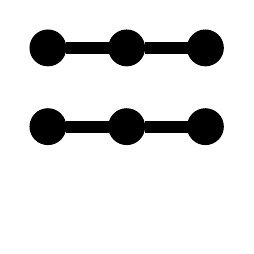
\begin{tikzpicture}
	\phantom{\draw (-0.25,-0.25) rectangle (2.25,2.25);}
	\node[draw,circle,fill=black,inner sep=0,outer sep=0,minimum size=3ex] (1) at (0,2) {};
	\node[draw,circle,fill=black,inner sep=0,outer sep=0,minimum size=3ex] (2) at (1,2) {};
	\node[draw,circle,fill=black,inner sep=0,outer sep=0,minimum size=3ex] (3) at (2,2) {};
	\node[draw,circle,fill=black,inner sep=0,outer sep=0,minimum size=3ex] (4) at (0,1) {};
	\node[draw,circle,fill=black,inner sep=0,outer sep=0,minimum size=3ex] (5) at (1,1) {};
	\node[draw,circle,fill=black,inner sep=0,outer sep=0,minimum size=3ex] (6) at (2,1) {};
	\draw[line width=1ex] (1) -- (2) -- (3);
	\draw[line width=1ex] (4) -- (5) -- (6);
\end{tikzpicture}
\newpage
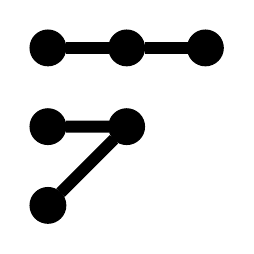
\begin{tikzpicture}
	\phantom{\draw (-0.25,-0.25) rectangle (2.25,2.25);}
	\node[draw,circle,fill=black,inner sep=0,outer sep=0,minimum size=3ex] (1) at (0,2) {};
	\node[draw,circle,fill=black,inner sep=0,outer sep=0,minimum size=3ex] (2) at (1,2) {};
	\node[draw,circle,fill=black,inner sep=0,outer sep=0,minimum size=3ex] (3) at (2,2) {};
	\node[draw,circle,fill=black,inner sep=0,outer sep=0,minimum size=3ex] (4) at (0,1) {};
	\node[draw,circle,fill=black,inner sep=0,outer sep=0,minimum size=3ex] (5) at (1,1) {};
	\node[draw,circle,fill=black,inner sep=0,outer sep=0,minimum size=3ex] (7) at (0,0) {};
	\draw[line width=1ex] (1) -- (2) -- (3);
	\draw[line width=1ex] (4) -- (5) -- (7);
\end{tikzpicture}
\newpage
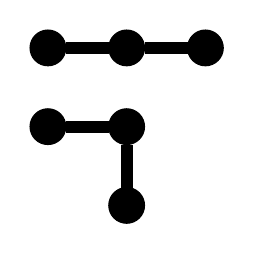
\begin{tikzpicture}
	\phantom{\draw (-0.25,-0.25) rectangle (2.25,2.25);}
	\node[draw,circle,fill=black,inner sep=0,outer sep=0,minimum size=3ex] (1) at (0,2) {};
	\node[draw,circle,fill=black,inner sep=0,outer sep=0,minimum size=3ex] (2) at (1,2) {};
	\node[draw,circle,fill=black,inner sep=0,outer sep=0,minimum size=3ex] (3) at (2,2) {};
	\node[draw,circle,fill=black,inner sep=0,outer sep=0,minimum size=3ex] (4) at (0,1) {};
	\node[draw,circle,fill=black,inner sep=0,outer sep=0,minimum size=3ex] (5) at (1,1) {};
	\node[draw,circle,fill=black,inner sep=0,outer sep=0,minimum size=3ex] (8) at (1,0) {};
	\draw[line width=1ex] (1) -- (2) -- (3);
	\draw[line width=1ex] (4) -- (5) -- (8);
\end{tikzpicture}
\newpage
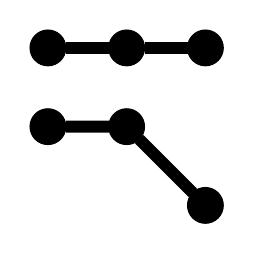
\begin{tikzpicture}
	\phantom{\draw (-0.25,-0.25) rectangle (2.25,2.25);}
	\node[draw,circle,fill=black,inner sep=0,outer sep=0,minimum size=3ex] (1) at (0,2) {};
	\node[draw,circle,fill=black,inner sep=0,outer sep=0,minimum size=3ex] (2) at (1,2) {};
	\node[draw,circle,fill=black,inner sep=0,outer sep=0,minimum size=3ex] (3) at (2,2) {};
	\node[draw,circle,fill=black,inner sep=0,outer sep=0,minimum size=3ex] (4) at (0,1) {};
	\node[draw,circle,fill=black,inner sep=0,outer sep=0,minimum size=3ex] (5) at (1,1) {};
	\node[draw,circle,fill=black,inner sep=0,outer sep=0,minimum size=3ex] (9) at (2,0) {};
	\draw[line width=1ex] (1) -- (2) -- (3);
	\draw[line width=1ex] (4) -- (5) -- (9);
\end{tikzpicture}
\newpage
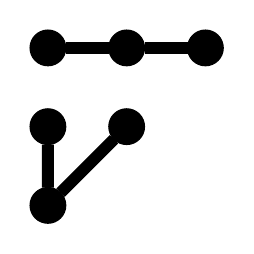
\begin{tikzpicture}
	\phantom{\draw (-0.25,-0.25) rectangle (2.25,2.25);}
	\node[draw,circle,fill=black,inner sep=0,outer sep=0,minimum size=3ex] (1) at (0,2) {};
	\node[draw,circle,fill=black,inner sep=0,outer sep=0,minimum size=3ex] (2) at (1,2) {};
	\node[draw,circle,fill=black,inner sep=0,outer sep=0,minimum size=3ex] (3) at (2,2) {};
	\node[draw,circle,fill=black,inner sep=0,outer sep=0,minimum size=3ex] (4) at (0,1) {};
	\node[draw,circle,fill=black,inner sep=0,outer sep=0,minimum size=3ex] (7) at (0,0) {};
	\node[draw,circle,fill=black,inner sep=0,outer sep=0,minimum size=3ex] (5) at (1,1) {};
	\draw[line width=1ex] (1) -- (2) -- (3);
	\draw[line width=1ex] (4) -- (7) -- (5);
\end{tikzpicture}
\newpage
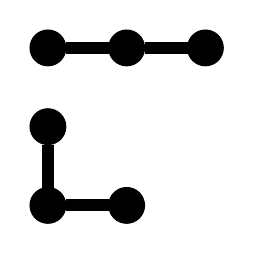
\begin{tikzpicture}
	\phantom{\draw (-0.25,-0.25) rectangle (2.25,2.25);}
	\node[draw,circle,fill=black,inner sep=0,outer sep=0,minimum size=3ex] (1) at (0,2) {};
	\node[draw,circle,fill=black,inner sep=0,outer sep=0,minimum size=3ex] (2) at (1,2) {};
	\node[draw,circle,fill=black,inner sep=0,outer sep=0,minimum size=3ex] (3) at (2,2) {};
	\node[draw,circle,fill=black,inner sep=0,outer sep=0,minimum size=3ex] (4) at (0,1) {};
	\node[draw,circle,fill=black,inner sep=0,outer sep=0,minimum size=3ex] (7) at (0,0) {};
	\node[draw,circle,fill=black,inner sep=0,outer sep=0,minimum size=3ex] (8) at (1,0) {};
	\draw[line width=1ex] (1) -- (2) -- (3);
	\draw[line width=1ex] (4) -- (7) -- (8);
\end{tikzpicture}
\newpage
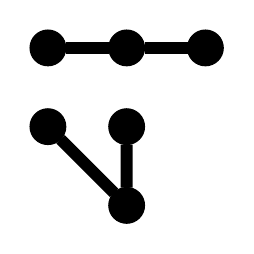
\begin{tikzpicture}
	\phantom{\draw (-0.25,-0.25) rectangle (2.25,2.25);}
	\node[draw,circle,fill=black,inner sep=0,outer sep=0,minimum size=3ex] (1) at (0,2) {};
	\node[draw,circle,fill=black,inner sep=0,outer sep=0,minimum size=3ex] (2) at (1,2) {};
	\node[draw,circle,fill=black,inner sep=0,outer sep=0,minimum size=3ex] (3) at (2,2) {};
	\node[draw,circle,fill=black,inner sep=0,outer sep=0,minimum size=3ex] (4) at (0,1) {};
	\node[draw,circle,fill=black,inner sep=0,outer sep=0,minimum size=3ex] (8) at (1,0) {};
	\node[draw,circle,fill=black,inner sep=0,outer sep=0,minimum size=3ex] (5) at (1,1) {};
	\draw[line width=1ex] (1) -- (2) -- (3);
	\draw[line width=1ex] (4) -- (8) -- (5);
\end{tikzpicture}
\newpage
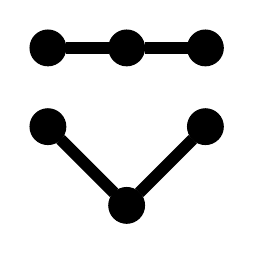
\begin{tikzpicture}
	\phantom{\draw (-0.25,-0.25) rectangle (2.25,2.25);}
	\node[draw,circle,fill=black,inner sep=0,outer sep=0,minimum size=3ex] (1) at (0,2) {};
	\node[draw,circle,fill=black,inner sep=0,outer sep=0,minimum size=3ex] (2) at (1,2) {};
	\node[draw,circle,fill=black,inner sep=0,outer sep=0,minimum size=3ex] (3) at (2,2) {};
	\node[draw,circle,fill=black,inner sep=0,outer sep=0,minimum size=3ex] (4) at (0,1) {};
	\node[draw,circle,fill=black,inner sep=0,outer sep=0,minimum size=3ex] (8) at (1,0) {};
	\node[draw,circle,fill=black,inner sep=0,outer sep=0,minimum size=3ex] (6) at (2,1) {};
	\draw[line width=1ex] (1) -- (2) -- (3);
	\draw[line width=1ex] (4) -- (8) -- (6);
\end{tikzpicture}
\newpage
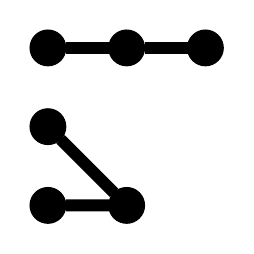
\begin{tikzpicture}
	\phantom{\draw (-0.25,-0.25) rectangle (2.25,2.25);}
	\node[draw,circle,fill=black,inner sep=0,outer sep=0,minimum size=3ex] (1) at (0,2) {};
	\node[draw,circle,fill=black,inner sep=0,outer sep=0,minimum size=3ex] (2) at (1,2) {};
	\node[draw,circle,fill=black,inner sep=0,outer sep=0,minimum size=3ex] (3) at (2,2) {};
	\node[draw,circle,fill=black,inner sep=0,outer sep=0,minimum size=3ex] (4) at (0,1) {};
	\node[draw,circle,fill=black,inner sep=0,outer sep=0,minimum size=3ex] (8) at (1,0) {};
	\node[draw,circle,fill=black,inner sep=0,outer sep=0,minimum size=3ex] (7) at (0,0) {};
	\draw[line width=1ex] (1) -- (2) -- (3);
	\draw[line width=1ex] (4) -- (8) -- (7);
\end{tikzpicture}
\newpage
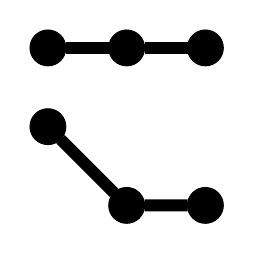
\begin{tikzpicture}
	\phantom{\draw (-0.25,-0.25) rectangle (2.25,2.25);}
	\node[draw,circle,fill=black,inner sep=0,outer sep=0,minimum size=3ex] (1) at (0,2) {};
	\node[draw,circle,fill=black,inner sep=0,outer sep=0,minimum size=3ex] (2) at (1,2) {};
	\node[draw,circle,fill=black,inner sep=0,outer sep=0,minimum size=3ex] (3) at (2,2) {};
	\node[draw,circle,fill=black,inner sep=0,outer sep=0,minimum size=3ex] (4) at (0,1) {};
	\node[draw,circle,fill=black,inner sep=0,outer sep=0,minimum size=3ex] (8) at (1,0) {};
	\node[draw,circle,fill=black,inner sep=0,outer sep=0,minimum size=3ex] (9) at (2,0) {};
	\draw[line width=1ex] (1) -- (2) -- (3);
	\draw[line width=1ex] (4) -- (8) -- (9);
\end{tikzpicture}
\newpage
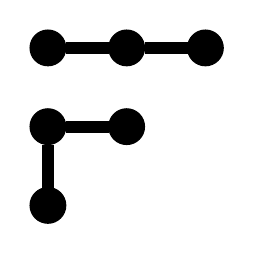
\begin{tikzpicture}
	\phantom{\draw (-0.25,-0.25) rectangle (2.25,2.25);}
	\node[draw,circle,fill=black,inner sep=0,outer sep=0,minimum size=3ex] (1) at (0,2) {};
	\node[draw,circle,fill=black,inner sep=0,outer sep=0,minimum size=3ex] (2) at (1,2) {};
	\node[draw,circle,fill=black,inner sep=0,outer sep=0,minimum size=3ex] (3) at (2,2) {};
	\node[draw,circle,fill=black,inner sep=0,outer sep=0,minimum size=3ex] (5) at (1,1) {};
	\node[draw,circle,fill=black,inner sep=0,outer sep=0,minimum size=3ex] (4) at (0,1) {};
	\node[draw,circle,fill=black,inner sep=0,outer sep=0,minimum size=3ex] (7) at (0,0) {};
	\draw[line width=1ex] (1) -- (2) -- (3);
	\draw[line width=1ex] (5) -- (4) -- (7);
\end{tikzpicture}
\newpage
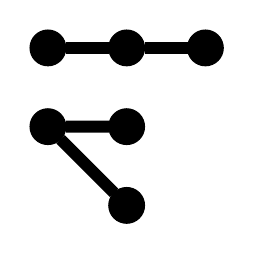
\begin{tikzpicture}
	\phantom{\draw (-0.25,-0.25) rectangle (2.25,2.25);}
	\node[draw,circle,fill=black,inner sep=0,outer sep=0,minimum size=3ex] (1) at (0,2) {};
	\node[draw,circle,fill=black,inner sep=0,outer sep=0,minimum size=3ex] (2) at (1,2) {};
	\node[draw,circle,fill=black,inner sep=0,outer sep=0,minimum size=3ex] (3) at (2,2) {};
	\node[draw,circle,fill=black,inner sep=0,outer sep=0,minimum size=3ex] (5) at (1,1) {};
	\node[draw,circle,fill=black,inner sep=0,outer sep=0,minimum size=3ex] (4) at (0,1) {};
	\node[draw,circle,fill=black,inner sep=0,outer sep=0,minimum size=3ex] (8) at (1,0) {};
	\draw[line width=1ex] (1) -- (2) -- (3);
	\draw[line width=1ex] (5) -- (4) -- (8);
\end{tikzpicture}
\newpage
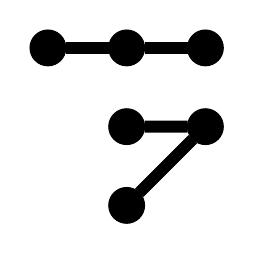
\begin{tikzpicture}
	\phantom{\draw (-0.25,-0.25) rectangle (2.25,2.25);}
	\node[draw,circle,fill=black,inner sep=0,outer sep=0,minimum size=3ex] (1) at (0,2) {};
	\node[draw,circle,fill=black,inner sep=0,outer sep=0,minimum size=3ex] (2) at (1,2) {};
	\node[draw,circle,fill=black,inner sep=0,outer sep=0,minimum size=3ex] (3) at (2,2) {};
	\node[draw,circle,fill=black,inner sep=0,outer sep=0,minimum size=3ex] (5) at (1,1) {};
	\node[draw,circle,fill=black,inner sep=0,outer sep=0,minimum size=3ex] (6) at (2,1) {};
	\node[draw,circle,fill=black,inner sep=0,outer sep=0,minimum size=3ex] (8) at (1,0) {};
	\draw[line width=1ex] (1) -- (2) -- (3);
	\draw[line width=1ex] (5) -- (6) -- (8);
\end{tikzpicture}
\newpage
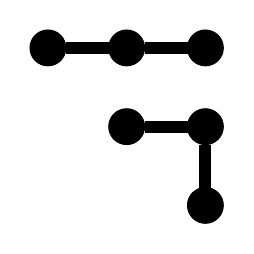
\begin{tikzpicture}
	\phantom{\draw (-0.25,-0.25) rectangle (2.25,2.25);}
	\node[draw,circle,fill=black,inner sep=0,outer sep=0,minimum size=3ex] (1) at (0,2) {};
	\node[draw,circle,fill=black,inner sep=0,outer sep=0,minimum size=3ex] (2) at (1,2) {};
	\node[draw,circle,fill=black,inner sep=0,outer sep=0,minimum size=3ex] (3) at (2,2) {};
	\node[draw,circle,fill=black,inner sep=0,outer sep=0,minimum size=3ex] (5) at (1,1) {};
	\node[draw,circle,fill=black,inner sep=0,outer sep=0,minimum size=3ex] (6) at (2,1) {};
	\node[draw,circle,fill=black,inner sep=0,outer sep=0,minimum size=3ex] (9) at (2,0) {};
	\draw[line width=1ex] (1) -- (2) -- (3);
	\draw[line width=1ex] (5) -- (6) -- (9);
\end{tikzpicture}
\newpage
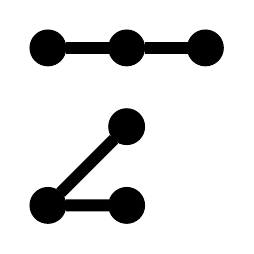
\begin{tikzpicture}
	\phantom{\draw (-0.25,-0.25) rectangle (2.25,2.25);}
	\node[draw,circle,fill=black,inner sep=0,outer sep=0,minimum size=3ex] (1) at (0,2) {};
	\node[draw,circle,fill=black,inner sep=0,outer sep=0,minimum size=3ex] (2) at (1,2) {};
	\node[draw,circle,fill=black,inner sep=0,outer sep=0,minimum size=3ex] (3) at (2,2) {};
	\node[draw,circle,fill=black,inner sep=0,outer sep=0,minimum size=3ex] (5) at (1,1) {};
	\node[draw,circle,fill=black,inner sep=0,outer sep=0,minimum size=3ex] (7) at (0,0) {};
	\node[draw,circle,fill=black,inner sep=0,outer sep=0,minimum size=3ex] (8) at (1,0) {};
	\draw[line width=1ex] (1) -- (2) -- (3);
	\draw[line width=1ex] (5) -- (7) -- (8);
\end{tikzpicture}
\newpage
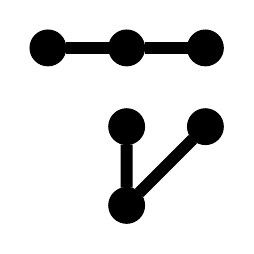
\begin{tikzpicture}
	\phantom{\draw (-0.25,-0.25) rectangle (2.25,2.25);}
	\node[draw,circle,fill=black,inner sep=0,outer sep=0,minimum size=3ex] (1) at (0,2) {};
	\node[draw,circle,fill=black,inner sep=0,outer sep=0,minimum size=3ex] (2) at (1,2) {};
	\node[draw,circle,fill=black,inner sep=0,outer sep=0,minimum size=3ex] (3) at (2,2) {};
	\node[draw,circle,fill=black,inner sep=0,outer sep=0,minimum size=3ex] (5) at (1,1) {};
	\node[draw,circle,fill=black,inner sep=0,outer sep=0,minimum size=3ex] (8) at (1,0) {};
	\node[draw,circle,fill=black,inner sep=0,outer sep=0,minimum size=3ex] (6) at (2,1) {};
	\draw[line width=1ex] (1) -- (2) -- (3);
	\draw[line width=1ex] (5) -- (8) -- (6);
\end{tikzpicture}
\newpage
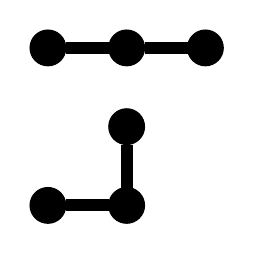
\begin{tikzpicture}
	\phantom{\draw (-0.25,-0.25) rectangle (2.25,2.25);}
	\node[draw,circle,fill=black,inner sep=0,outer sep=0,minimum size=3ex] (1) at (0,2) {};
	\node[draw,circle,fill=black,inner sep=0,outer sep=0,minimum size=3ex] (2) at (1,2) {};
	\node[draw,circle,fill=black,inner sep=0,outer sep=0,minimum size=3ex] (3) at (2,2) {};
	\node[draw,circle,fill=black,inner sep=0,outer sep=0,minimum size=3ex] (5) at (1,1) {};
	\node[draw,circle,fill=black,inner sep=0,outer sep=0,minimum size=3ex] (8) at (1,0) {};
	\node[draw,circle,fill=black,inner sep=0,outer sep=0,minimum size=3ex] (7) at (0,0) {};
	\draw[line width=1ex] (1) -- (2) -- (3);
	\draw[line width=1ex] (5) -- (8) -- (7);
\end{tikzpicture}
\newpage
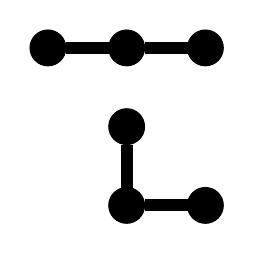
\begin{tikzpicture}
	\phantom{\draw (-0.25,-0.25) rectangle (2.25,2.25);}
	\node[draw,circle,fill=black,inner sep=0,outer sep=0,minimum size=3ex] (1) at (0,2) {};
	\node[draw,circle,fill=black,inner sep=0,outer sep=0,minimum size=3ex] (2) at (1,2) {};
	\node[draw,circle,fill=black,inner sep=0,outer sep=0,minimum size=3ex] (3) at (2,2) {};
	\node[draw,circle,fill=black,inner sep=0,outer sep=0,minimum size=3ex] (5) at (1,1) {};
	\node[draw,circle,fill=black,inner sep=0,outer sep=0,minimum size=3ex] (8) at (1,0) {};
	\node[draw,circle,fill=black,inner sep=0,outer sep=0,minimum size=3ex] (9) at (2,0) {};
	\draw[line width=1ex] (1) -- (2) -- (3);
	\draw[line width=1ex] (5) -- (8) -- (9);
\end{tikzpicture}
\newpage
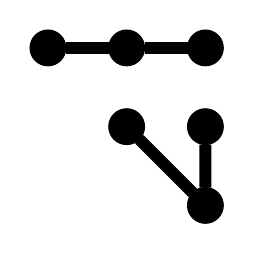
\begin{tikzpicture}
	\phantom{\draw (-0.25,-0.25) rectangle (2.25,2.25);}
	\node[draw,circle,fill=black,inner sep=0,outer sep=0,minimum size=3ex] (1) at (0,2) {};
	\node[draw,circle,fill=black,inner sep=0,outer sep=0,minimum size=3ex] (2) at (1,2) {};
	\node[draw,circle,fill=black,inner sep=0,outer sep=0,minimum size=3ex] (3) at (2,2) {};
	\node[draw,circle,fill=black,inner sep=0,outer sep=0,minimum size=3ex] (5) at (1,1) {};
	\node[draw,circle,fill=black,inner sep=0,outer sep=0,minimum size=3ex] (9) at (2,0) {};
	\node[draw,circle,fill=black,inner sep=0,outer sep=0,minimum size=3ex] (6) at (2,1) {};
	\draw[line width=1ex] (1) -- (2) -- (3);
	\draw[line width=1ex] (5) -- (9) -- (6);
\end{tikzpicture}
\newpage
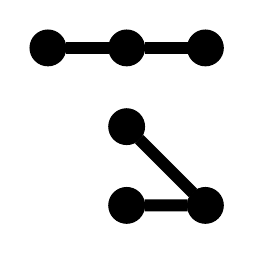
\begin{tikzpicture}
	\phantom{\draw (-0.25,-0.25) rectangle (2.25,2.25);}
	\node[draw,circle,fill=black,inner sep=0,outer sep=0,minimum size=3ex] (1) at (0,2) {};
	\node[draw,circle,fill=black,inner sep=0,outer sep=0,minimum size=3ex] (2) at (1,2) {};
	\node[draw,circle,fill=black,inner sep=0,outer sep=0,minimum size=3ex] (3) at (2,2) {};
	\node[draw,circle,fill=black,inner sep=0,outer sep=0,minimum size=3ex] (5) at (1,1) {};
	\node[draw,circle,fill=black,inner sep=0,outer sep=0,minimum size=3ex] (9) at (2,0) {};
	\node[draw,circle,fill=black,inner sep=0,outer sep=0,minimum size=3ex] (8) at (1,0) {};
	\draw[line width=1ex] (1) -- (2) -- (3);
	\draw[line width=1ex] (5) -- (9) -- (8);
\end{tikzpicture}
\newpage
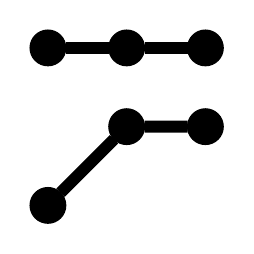
\begin{tikzpicture}
	\phantom{\draw (-0.25,-0.25) rectangle (2.25,2.25);}
	\node[draw,circle,fill=black,inner sep=0,outer sep=0,minimum size=3ex] (1) at (0,2) {};
	\node[draw,circle,fill=black,inner sep=0,outer sep=0,minimum size=3ex] (2) at (1,2) {};
	\node[draw,circle,fill=black,inner sep=0,outer sep=0,minimum size=3ex] (3) at (2,2) {};
	\node[draw,circle,fill=black,inner sep=0,outer sep=0,minimum size=3ex] (6) at (2,1) {};
	\node[draw,circle,fill=black,inner sep=0,outer sep=0,minimum size=3ex] (5) at (1,1) {};
	\node[draw,circle,fill=black,inner sep=0,outer sep=0,minimum size=3ex] (7) at (0,0) {};
	\draw[line width=1ex] (1) -- (2) -- (3);
	\draw[line width=1ex] (6) -- (5) -- (7);
\end{tikzpicture}
\newpage
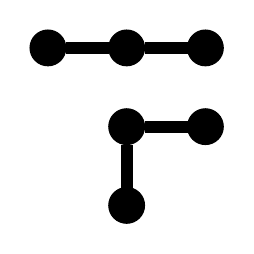
\begin{tikzpicture}
	\phantom{\draw (-0.25,-0.25) rectangle (2.25,2.25);}
	\node[draw,circle,fill=black,inner sep=0,outer sep=0,minimum size=3ex] (1) at (0,2) {};
	\node[draw,circle,fill=black,inner sep=0,outer sep=0,minimum size=3ex] (2) at (1,2) {};
	\node[draw,circle,fill=black,inner sep=0,outer sep=0,minimum size=3ex] (3) at (2,2) {};
	\node[draw,circle,fill=black,inner sep=0,outer sep=0,minimum size=3ex] (6) at (2,1) {};
	\node[draw,circle,fill=black,inner sep=0,outer sep=0,minimum size=3ex] (5) at (1,1) {};
	\node[draw,circle,fill=black,inner sep=0,outer sep=0,minimum size=3ex] (8) at (1,0) {};
	\draw[line width=1ex] (1) -- (2) -- (3);
	\draw[line width=1ex] (6) -- (5) -- (8);
\end{tikzpicture}
\newpage
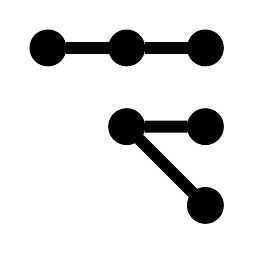
\begin{tikzpicture}
	\phantom{\draw (-0.25,-0.25) rectangle (2.25,2.25);}
	\node[draw,circle,fill=black,inner sep=0,outer sep=0,minimum size=3ex] (1) at (0,2) {};
	\node[draw,circle,fill=black,inner sep=0,outer sep=0,minimum size=3ex] (2) at (1,2) {};
	\node[draw,circle,fill=black,inner sep=0,outer sep=0,minimum size=3ex] (3) at (2,2) {};
	\node[draw,circle,fill=black,inner sep=0,outer sep=0,minimum size=3ex] (6) at (2,1) {};
	\node[draw,circle,fill=black,inner sep=0,outer sep=0,minimum size=3ex] (5) at (1,1) {};
	\node[draw,circle,fill=black,inner sep=0,outer sep=0,minimum size=3ex] (9) at (2,0) {};
	\draw[line width=1ex] (1) -- (2) -- (3);
	\draw[line width=1ex] (6) -- (5) -- (9);
\end{tikzpicture}
\newpage
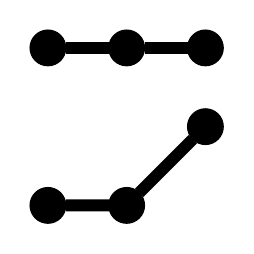
\begin{tikzpicture}
	\phantom{\draw (-0.25,-0.25) rectangle (2.25,2.25);}
	\node[draw,circle,fill=black,inner sep=0,outer sep=0,minimum size=3ex] (1) at (0,2) {};
	\node[draw,circle,fill=black,inner sep=0,outer sep=0,minimum size=3ex] (2) at (1,2) {};
	\node[draw,circle,fill=black,inner sep=0,outer sep=0,minimum size=3ex] (3) at (2,2) {};
	\node[draw,circle,fill=black,inner sep=0,outer sep=0,minimum size=3ex] (6) at (2,1) {};
	\node[draw,circle,fill=black,inner sep=0,outer sep=0,minimum size=3ex] (8) at (1,0) {};
	\node[draw,circle,fill=black,inner sep=0,outer sep=0,minimum size=3ex] (7) at (0,0) {};
	\draw[line width=1ex] (1) -- (2) -- (3);
	\draw[line width=1ex] (6) -- (8) -- (7);
\end{tikzpicture}
\newpage
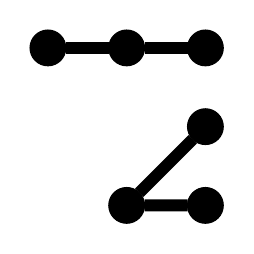
\begin{tikzpicture}
	\phantom{\draw (-0.25,-0.25) rectangle (2.25,2.25);}
	\node[draw,circle,fill=black,inner sep=0,outer sep=0,minimum size=3ex] (1) at (0,2) {};
	\node[draw,circle,fill=black,inner sep=0,outer sep=0,minimum size=3ex] (2) at (1,2) {};
	\node[draw,circle,fill=black,inner sep=0,outer sep=0,minimum size=3ex] (3) at (2,2) {};
	\node[draw,circle,fill=black,inner sep=0,outer sep=0,minimum size=3ex] (6) at (2,1) {};
	\node[draw,circle,fill=black,inner sep=0,outer sep=0,minimum size=3ex] (8) at (1,0) {};
	\node[draw,circle,fill=black,inner sep=0,outer sep=0,minimum size=3ex] (9) at (2,0) {};
	\draw[line width=1ex] (1) -- (2) -- (3);
	\draw[line width=1ex] (6) -- (8) -- (9);
\end{tikzpicture}
\newpage
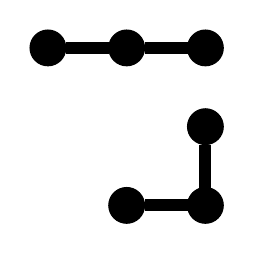
\begin{tikzpicture}
	\phantom{\draw (-0.25,-0.25) rectangle (2.25,2.25);}
	\node[draw,circle,fill=black,inner sep=0,outer sep=0,minimum size=3ex] (1) at (0,2) {};
	\node[draw,circle,fill=black,inner sep=0,outer sep=0,minimum size=3ex] (2) at (1,2) {};
	\node[draw,circle,fill=black,inner sep=0,outer sep=0,minimum size=3ex] (3) at (2,2) {};
	\node[draw,circle,fill=black,inner sep=0,outer sep=0,minimum size=3ex] (6) at (2,1) {};
	\node[draw,circle,fill=black,inner sep=0,outer sep=0,minimum size=3ex] (9) at (2,0) {};
	\node[draw,circle,fill=black,inner sep=0,outer sep=0,minimum size=3ex] (8) at (1,0) {};
	\draw[line width=1ex] (1) -- (2) -- (3);
	\draw[line width=1ex] (6) -- (9) -- (8);
\end{tikzpicture}
\newpage
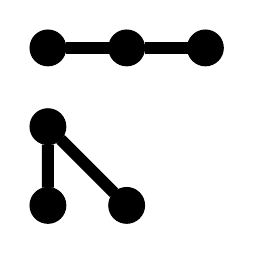
\begin{tikzpicture}
	\phantom{\draw (-0.25,-0.25) rectangle (2.25,2.25);}
	\node[draw,circle,fill=black,inner sep=0,outer sep=0,minimum size=3ex] (1) at (0,2) {};
	\node[draw,circle,fill=black,inner sep=0,outer sep=0,minimum size=3ex] (2) at (1,2) {};
	\node[draw,circle,fill=black,inner sep=0,outer sep=0,minimum size=3ex] (3) at (2,2) {};
	\node[draw,circle,fill=black,inner sep=0,outer sep=0,minimum size=3ex] (7) at (0,0) {};
	\node[draw,circle,fill=black,inner sep=0,outer sep=0,minimum size=3ex] (4) at (0,1) {};
	\node[draw,circle,fill=black,inner sep=0,outer sep=0,minimum size=3ex] (8) at (1,0) {};
	\draw[line width=1ex] (1) -- (2) -- (3);
	\draw[line width=1ex] (7) -- (4) -- (8);
\end{tikzpicture}
\newpage
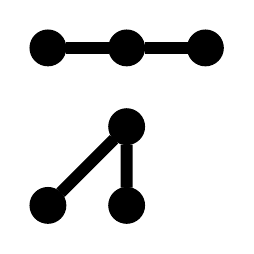
\begin{tikzpicture}
	\phantom{\draw (-0.25,-0.25) rectangle (2.25,2.25);}
	\node[draw,circle,fill=black,inner sep=0,outer sep=0,minimum size=3ex] (1) at (0,2) {};
	\node[draw,circle,fill=black,inner sep=0,outer sep=0,minimum size=3ex] (2) at (1,2) {};
	\node[draw,circle,fill=black,inner sep=0,outer sep=0,minimum size=3ex] (3) at (2,2) {};
	\node[draw,circle,fill=black,inner sep=0,outer sep=0,minimum size=3ex] (7) at (0,0) {};
	\node[draw,circle,fill=black,inner sep=0,outer sep=0,minimum size=3ex] (5) at (1,1) {};
	\node[draw,circle,fill=black,inner sep=0,outer sep=0,minimum size=3ex] (8) at (1,0) {};
	\draw[line width=1ex] (1) -- (2) -- (3);
	\draw[line width=1ex] (7) -- (5) -- (8);
\end{tikzpicture}
\newpage
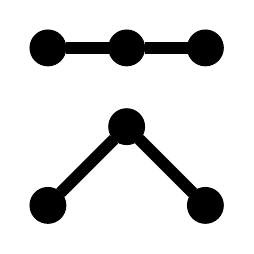
\begin{tikzpicture}
	\phantom{\draw (-0.25,-0.25) rectangle (2.25,2.25);}
	\node[draw,circle,fill=black,inner sep=0,outer sep=0,minimum size=3ex] (1) at (0,2) {};
	\node[draw,circle,fill=black,inner sep=0,outer sep=0,minimum size=3ex] (2) at (1,2) {};
	\node[draw,circle,fill=black,inner sep=0,outer sep=0,minimum size=3ex] (3) at (2,2) {};
	\node[draw,circle,fill=black,inner sep=0,outer sep=0,minimum size=3ex] (7) at (0,0) {};
	\node[draw,circle,fill=black,inner sep=0,outer sep=0,minimum size=3ex] (5) at (1,1) {};
	\node[draw,circle,fill=black,inner sep=0,outer sep=0,minimum size=3ex] (9) at (2,0) {};
	\draw[line width=1ex] (1) -- (2) -- (3);
	\draw[line width=1ex] (7) -- (5) -- (9);
\end{tikzpicture}
\newpage
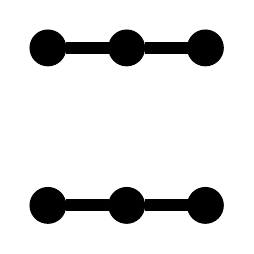
\begin{tikzpicture}
	\phantom{\draw (-0.25,-0.25) rectangle (2.25,2.25);}
	\node[draw,circle,fill=black,inner sep=0,outer sep=0,minimum size=3ex] (1) at (0,2) {};
	\node[draw,circle,fill=black,inner sep=0,outer sep=0,minimum size=3ex] (2) at (1,2) {};
	\node[draw,circle,fill=black,inner sep=0,outer sep=0,minimum size=3ex] (3) at (2,2) {};
	\node[draw,circle,fill=black,inner sep=0,outer sep=0,minimum size=3ex] (7) at (0,0) {};
	\node[draw,circle,fill=black,inner sep=0,outer sep=0,minimum size=3ex] (8) at (1,0) {};
	\node[draw,circle,fill=black,inner sep=0,outer sep=0,minimum size=3ex] (9) at (2,0) {};
	\draw[line width=1ex] (1) -- (2) -- (3);
	\draw[line width=1ex] (7) -- (8) -- (9);
\end{tikzpicture}
\newpage
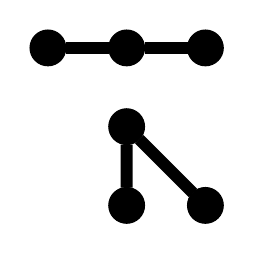
\begin{tikzpicture}
	\phantom{\draw (-0.25,-0.25) rectangle (2.25,2.25);}
	\node[draw,circle,fill=black,inner sep=0,outer sep=0,minimum size=3ex] (1) at (0,2) {};
	\node[draw,circle,fill=black,inner sep=0,outer sep=0,minimum size=3ex] (2) at (1,2) {};
	\node[draw,circle,fill=black,inner sep=0,outer sep=0,minimum size=3ex] (3) at (2,2) {};
	\node[draw,circle,fill=black,inner sep=0,outer sep=0,minimum size=3ex] (8) at (1,0) {};
	\node[draw,circle,fill=black,inner sep=0,outer sep=0,minimum size=3ex] (5) at (1,1) {};
	\node[draw,circle,fill=black,inner sep=0,outer sep=0,minimum size=3ex] (9) at (2,0) {};
	\draw[line width=1ex] (1) -- (2) -- (3);
	\draw[line width=1ex] (8) -- (5) -- (9);
\end{tikzpicture}
\newpage
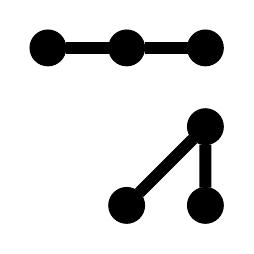
\begin{tikzpicture}
	\phantom{\draw (-0.25,-0.25) rectangle (2.25,2.25);}
	\node[draw,circle,fill=black,inner sep=0,outer sep=0,minimum size=3ex] (1) at (0,2) {};
	\node[draw,circle,fill=black,inner sep=0,outer sep=0,minimum size=3ex] (2) at (1,2) {};
	\node[draw,circle,fill=black,inner sep=0,outer sep=0,minimum size=3ex] (3) at (2,2) {};
	\node[draw,circle,fill=black,inner sep=0,outer sep=0,minimum size=3ex] (8) at (1,0) {};
	\node[draw,circle,fill=black,inner sep=0,outer sep=0,minimum size=3ex] (6) at (2,1) {};
	\node[draw,circle,fill=black,inner sep=0,outer sep=0,minimum size=3ex] (9) at (2,0) {};
	\draw[line width=1ex] (1) -- (2) -- (3);
	\draw[line width=1ex] (8) -- (6) -- (9);
\end{tikzpicture}
\newpage
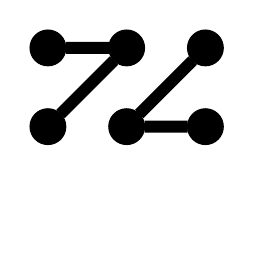
\begin{tikzpicture}
	\phantom{\draw (-0.25,-0.25) rectangle (2.25,2.25);}
	\node[draw,circle,fill=black,inner sep=0,outer sep=0,minimum size=3ex] (1) at (0,2) {};
	\node[draw,circle,fill=black,inner sep=0,outer sep=0,minimum size=3ex] (2) at (1,2) {};
	\node[draw,circle,fill=black,inner sep=0,outer sep=0,minimum size=3ex] (4) at (0,1) {};
	\node[draw,circle,fill=black,inner sep=0,outer sep=0,minimum size=3ex] (3) at (2,2) {};
	\node[draw,circle,fill=black,inner sep=0,outer sep=0,minimum size=3ex] (5) at (1,1) {};
	\node[draw,circle,fill=black,inner sep=0,outer sep=0,minimum size=3ex] (6) at (2,1) {};
	\draw[line width=1ex] (1) -- (2) -- (4);
	\draw[line width=1ex] (3) -- (5) -- (6);
\end{tikzpicture}
\newpage
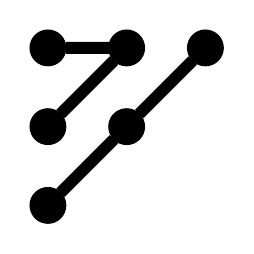
\begin{tikzpicture}
	\phantom{\draw (-0.25,-0.25) rectangle (2.25,2.25);}
	\node[draw,circle,fill=black,inner sep=0,outer sep=0,minimum size=3ex] (1) at (0,2) {};
	\node[draw,circle,fill=black,inner sep=0,outer sep=0,minimum size=3ex] (2) at (1,2) {};
	\node[draw,circle,fill=black,inner sep=0,outer sep=0,minimum size=3ex] (4) at (0,1) {};
	\node[draw,circle,fill=black,inner sep=0,outer sep=0,minimum size=3ex] (3) at (2,2) {};
	\node[draw,circle,fill=black,inner sep=0,outer sep=0,minimum size=3ex] (5) at (1,1) {};
	\node[draw,circle,fill=black,inner sep=0,outer sep=0,minimum size=3ex] (7) at (0,0) {};
	\draw[line width=1ex] (1) -- (2) -- (4);
	\draw[line width=1ex] (3) -- (5) -- (7);
\end{tikzpicture}
\newpage
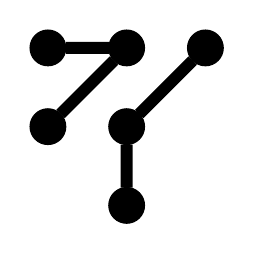
\begin{tikzpicture}
	\phantom{\draw (-0.25,-0.25) rectangle (2.25,2.25);}
	\node[draw,circle,fill=black,inner sep=0,outer sep=0,minimum size=3ex] (1) at (0,2) {};
	\node[draw,circle,fill=black,inner sep=0,outer sep=0,minimum size=3ex] (2) at (1,2) {};
	\node[draw,circle,fill=black,inner sep=0,outer sep=0,minimum size=3ex] (4) at (0,1) {};
	\node[draw,circle,fill=black,inner sep=0,outer sep=0,minimum size=3ex] (3) at (2,2) {};
	\node[draw,circle,fill=black,inner sep=0,outer sep=0,minimum size=3ex] (5) at (1,1) {};
	\node[draw,circle,fill=black,inner sep=0,outer sep=0,minimum size=3ex] (8) at (1,0) {};
	\draw[line width=1ex] (1) -- (2) -- (4);
	\draw[line width=1ex] (3) -- (5) -- (8);
\end{tikzpicture}
\newpage
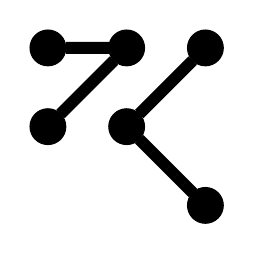
\begin{tikzpicture}
	\phantom{\draw (-0.25,-0.25) rectangle (2.25,2.25);}
	\node[draw,circle,fill=black,inner sep=0,outer sep=0,minimum size=3ex] (1) at (0,2) {};
	\node[draw,circle,fill=black,inner sep=0,outer sep=0,minimum size=3ex] (2) at (1,2) {};
	\node[draw,circle,fill=black,inner sep=0,outer sep=0,minimum size=3ex] (4) at (0,1) {};
	\node[draw,circle,fill=black,inner sep=0,outer sep=0,minimum size=3ex] (3) at (2,2) {};
	\node[draw,circle,fill=black,inner sep=0,outer sep=0,minimum size=3ex] (5) at (1,1) {};
	\node[draw,circle,fill=black,inner sep=0,outer sep=0,minimum size=3ex] (9) at (2,0) {};
	\draw[line width=1ex] (1) -- (2) -- (4);
	\draw[line width=1ex] (3) -- (5) -- (9);
\end{tikzpicture}
\newpage
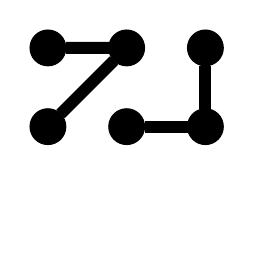
\begin{tikzpicture}
	\phantom{\draw (-0.25,-0.25) rectangle (2.25,2.25);}
	\node[draw,circle,fill=black,inner sep=0,outer sep=0,minimum size=3ex] (1) at (0,2) {};
	\node[draw,circle,fill=black,inner sep=0,outer sep=0,minimum size=3ex] (2) at (1,2) {};
	\node[draw,circle,fill=black,inner sep=0,outer sep=0,minimum size=3ex] (4) at (0,1) {};
	\node[draw,circle,fill=black,inner sep=0,outer sep=0,minimum size=3ex] (3) at (2,2) {};
	\node[draw,circle,fill=black,inner sep=0,outer sep=0,minimum size=3ex] (6) at (2,1) {};
	\node[draw,circle,fill=black,inner sep=0,outer sep=0,minimum size=3ex] (5) at (1,1) {};
	\draw[line width=1ex] (1) -- (2) -- (4);
	\draw[line width=1ex] (3) -- (6) -- (5);
\end{tikzpicture}
\newpage
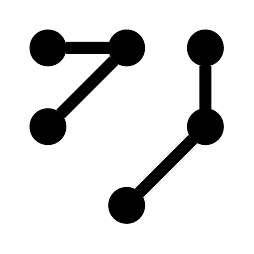
\begin{tikzpicture}
	\phantom{\draw (-0.25,-0.25) rectangle (2.25,2.25);}
	\node[draw,circle,fill=black,inner sep=0,outer sep=0,minimum size=3ex] (1) at (0,2) {};
	\node[draw,circle,fill=black,inner sep=0,outer sep=0,minimum size=3ex] (2) at (1,2) {};
	\node[draw,circle,fill=black,inner sep=0,outer sep=0,minimum size=3ex] (4) at (0,1) {};
	\node[draw,circle,fill=black,inner sep=0,outer sep=0,minimum size=3ex] (3) at (2,2) {};
	\node[draw,circle,fill=black,inner sep=0,outer sep=0,minimum size=3ex] (6) at (2,1) {};
	\node[draw,circle,fill=black,inner sep=0,outer sep=0,minimum size=3ex] (8) at (1,0) {};
	\draw[line width=1ex] (1) -- (2) -- (4);
	\draw[line width=1ex] (3) -- (6) -- (8);
\end{tikzpicture}
\newpage
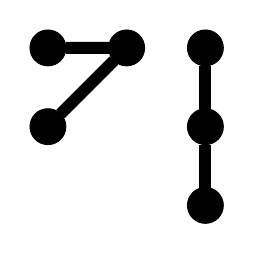
\begin{tikzpicture}
	\phantom{\draw (-0.25,-0.25) rectangle (2.25,2.25);}
	\node[draw,circle,fill=black,inner sep=0,outer sep=0,minimum size=3ex] (1) at (0,2) {};
	\node[draw,circle,fill=black,inner sep=0,outer sep=0,minimum size=3ex] (2) at (1,2) {};
	\node[draw,circle,fill=black,inner sep=0,outer sep=0,minimum size=3ex] (4) at (0,1) {};
	\node[draw,circle,fill=black,inner sep=0,outer sep=0,minimum size=3ex] (3) at (2,2) {};
	\node[draw,circle,fill=black,inner sep=0,outer sep=0,minimum size=3ex] (6) at (2,1) {};
	\node[draw,circle,fill=black,inner sep=0,outer sep=0,minimum size=3ex] (9) at (2,0) {};
	\draw[line width=1ex] (1) -- (2) -- (4);
	\draw[line width=1ex] (3) -- (6) -- (9);
\end{tikzpicture}
\newpage
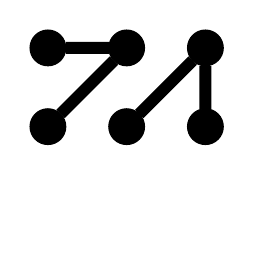
\begin{tikzpicture}
	\phantom{\draw (-0.25,-0.25) rectangle (2.25,2.25);}
	\node[draw,circle,fill=black,inner sep=0,outer sep=0,minimum size=3ex] (1) at (0,2) {};
	\node[draw,circle,fill=black,inner sep=0,outer sep=0,minimum size=3ex] (2) at (1,2) {};
	\node[draw,circle,fill=black,inner sep=0,outer sep=0,minimum size=3ex] (4) at (0,1) {};
	\node[draw,circle,fill=black,inner sep=0,outer sep=0,minimum size=3ex] (5) at (1,1) {};
	\node[draw,circle,fill=black,inner sep=0,outer sep=0,minimum size=3ex] (3) at (2,2) {};
	\node[draw,circle,fill=black,inner sep=0,outer sep=0,minimum size=3ex] (6) at (2,1) {};
	\draw[line width=1ex] (1) -- (2) -- (4);
	\draw[line width=1ex] (5) -- (3) -- (6);
\end{tikzpicture}
\newpage
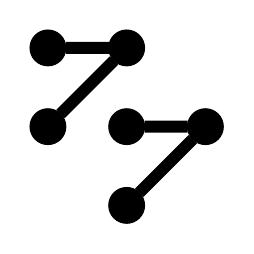
\begin{tikzpicture}
	\phantom{\draw (-0.25,-0.25) rectangle (2.25,2.25);}
	\node[draw,circle,fill=black,inner sep=0,outer sep=0,minimum size=3ex] (1) at (0,2) {};
	\node[draw,circle,fill=black,inner sep=0,outer sep=0,minimum size=3ex] (2) at (1,2) {};
	\node[draw,circle,fill=black,inner sep=0,outer sep=0,minimum size=3ex] (4) at (0,1) {};
	\node[draw,circle,fill=black,inner sep=0,outer sep=0,minimum size=3ex] (5) at (1,1) {};
	\node[draw,circle,fill=black,inner sep=0,outer sep=0,minimum size=3ex] (6) at (2,1) {};
	\node[draw,circle,fill=black,inner sep=0,outer sep=0,minimum size=3ex] (8) at (1,0) {};
	\draw[line width=1ex] (1) -- (2) -- (4);
	\draw[line width=1ex] (5) -- (6) -- (8);
\end{tikzpicture}
\newpage
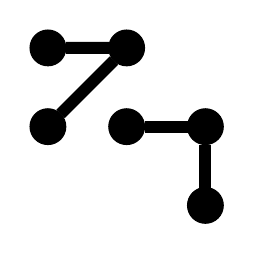
\begin{tikzpicture}
	\phantom{\draw (-0.25,-0.25) rectangle (2.25,2.25);}
	\node[draw,circle,fill=black,inner sep=0,outer sep=0,minimum size=3ex] (1) at (0,2) {};
	\node[draw,circle,fill=black,inner sep=0,outer sep=0,minimum size=3ex] (2) at (1,2) {};
	\node[draw,circle,fill=black,inner sep=0,outer sep=0,minimum size=3ex] (4) at (0,1) {};
	\node[draw,circle,fill=black,inner sep=0,outer sep=0,minimum size=3ex] (5) at (1,1) {};
	\node[draw,circle,fill=black,inner sep=0,outer sep=0,minimum size=3ex] (6) at (2,1) {};
	\node[draw,circle,fill=black,inner sep=0,outer sep=0,minimum size=3ex] (9) at (2,0) {};
	\draw[line width=1ex] (1) -- (2) -- (4);
	\draw[line width=1ex] (5) -- (6) -- (9);
\end{tikzpicture}
\newpage
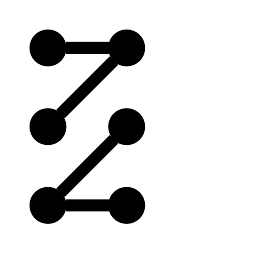
\begin{tikzpicture}
	\phantom{\draw (-0.25,-0.25) rectangle (2.25,2.25);}
	\node[draw,circle,fill=black,inner sep=0,outer sep=0,minimum size=3ex] (1) at (0,2) {};
	\node[draw,circle,fill=black,inner sep=0,outer sep=0,minimum size=3ex] (2) at (1,2) {};
	\node[draw,circle,fill=black,inner sep=0,outer sep=0,minimum size=3ex] (4) at (0,1) {};
	\node[draw,circle,fill=black,inner sep=0,outer sep=0,minimum size=3ex] (5) at (1,1) {};
	\node[draw,circle,fill=black,inner sep=0,outer sep=0,minimum size=3ex] (7) at (0,0) {};
	\node[draw,circle,fill=black,inner sep=0,outer sep=0,minimum size=3ex] (8) at (1,0) {};
	\draw[line width=1ex] (1) -- (2) -- (4);
	\draw[line width=1ex] (5) -- (7) -- (8);
\end{tikzpicture}
\newpage
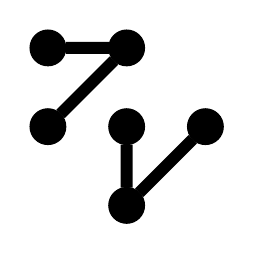
\begin{tikzpicture}
	\phantom{\draw (-0.25,-0.25) rectangle (2.25,2.25);}
	\node[draw,circle,fill=black,inner sep=0,outer sep=0,minimum size=3ex] (1) at (0,2) {};
	\node[draw,circle,fill=black,inner sep=0,outer sep=0,minimum size=3ex] (2) at (1,2) {};
	\node[draw,circle,fill=black,inner sep=0,outer sep=0,minimum size=3ex] (4) at (0,1) {};
	\node[draw,circle,fill=black,inner sep=0,outer sep=0,minimum size=3ex] (5) at (1,1) {};
	\node[draw,circle,fill=black,inner sep=0,outer sep=0,minimum size=3ex] (8) at (1,0) {};
	\node[draw,circle,fill=black,inner sep=0,outer sep=0,minimum size=3ex] (6) at (2,1) {};
	\draw[line width=1ex] (1) -- (2) -- (4);
	\draw[line width=1ex] (5) -- (8) -- (6);
\end{tikzpicture}
\newpage
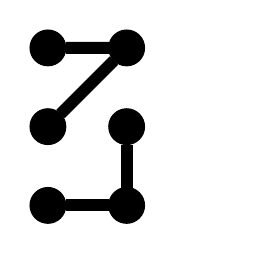
\begin{tikzpicture}
	\phantom{\draw (-0.25,-0.25) rectangle (2.25,2.25);}
	\node[draw,circle,fill=black,inner sep=0,outer sep=0,minimum size=3ex] (1) at (0,2) {};
	\node[draw,circle,fill=black,inner sep=0,outer sep=0,minimum size=3ex] (2) at (1,2) {};
	\node[draw,circle,fill=black,inner sep=0,outer sep=0,minimum size=3ex] (4) at (0,1) {};
	\node[draw,circle,fill=black,inner sep=0,outer sep=0,minimum size=3ex] (5) at (1,1) {};
	\node[draw,circle,fill=black,inner sep=0,outer sep=0,minimum size=3ex] (8) at (1,0) {};
	\node[draw,circle,fill=black,inner sep=0,outer sep=0,minimum size=3ex] (7) at (0,0) {};
	\draw[line width=1ex] (1) -- (2) -- (4);
	\draw[line width=1ex] (5) -- (8) -- (7);
\end{tikzpicture}
\newpage
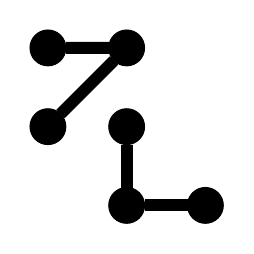
\begin{tikzpicture}
	\phantom{\draw (-0.25,-0.25) rectangle (2.25,2.25);}
	\node[draw,circle,fill=black,inner sep=0,outer sep=0,minimum size=3ex] (1) at (0,2) {};
	\node[draw,circle,fill=black,inner sep=0,outer sep=0,minimum size=3ex] (2) at (1,2) {};
	\node[draw,circle,fill=black,inner sep=0,outer sep=0,minimum size=3ex] (4) at (0,1) {};
	\node[draw,circle,fill=black,inner sep=0,outer sep=0,minimum size=3ex] (5) at (1,1) {};
	\node[draw,circle,fill=black,inner sep=0,outer sep=0,minimum size=3ex] (8) at (1,0) {};
	\node[draw,circle,fill=black,inner sep=0,outer sep=0,minimum size=3ex] (9) at (2,0) {};
	\draw[line width=1ex] (1) -- (2) -- (4);
	\draw[line width=1ex] (5) -- (8) -- (9);
\end{tikzpicture}
\newpage
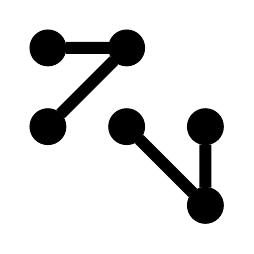
\begin{tikzpicture}
	\phantom{\draw (-0.25,-0.25) rectangle (2.25,2.25);}
	\node[draw,circle,fill=black,inner sep=0,outer sep=0,minimum size=3ex] (1) at (0,2) {};
	\node[draw,circle,fill=black,inner sep=0,outer sep=0,minimum size=3ex] (2) at (1,2) {};
	\node[draw,circle,fill=black,inner sep=0,outer sep=0,minimum size=3ex] (4) at (0,1) {};
	\node[draw,circle,fill=black,inner sep=0,outer sep=0,minimum size=3ex] (5) at (1,1) {};
	\node[draw,circle,fill=black,inner sep=0,outer sep=0,minimum size=3ex] (9) at (2,0) {};
	\node[draw,circle,fill=black,inner sep=0,outer sep=0,minimum size=3ex] (6) at (2,1) {};
	\draw[line width=1ex] (1) -- (2) -- (4);
	\draw[line width=1ex] (5) -- (9) -- (6);
\end{tikzpicture}
\newpage
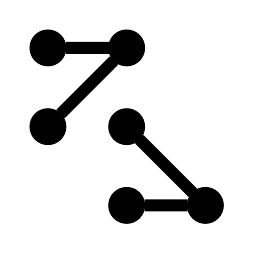
\begin{tikzpicture}
	\phantom{\draw (-0.25,-0.25) rectangle (2.25,2.25);}
	\node[draw,circle,fill=black,inner sep=0,outer sep=0,minimum size=3ex] (1) at (0,2) {};
	\node[draw,circle,fill=black,inner sep=0,outer sep=0,minimum size=3ex] (2) at (1,2) {};
	\node[draw,circle,fill=black,inner sep=0,outer sep=0,minimum size=3ex] (4) at (0,1) {};
	\node[draw,circle,fill=black,inner sep=0,outer sep=0,minimum size=3ex] (5) at (1,1) {};
	\node[draw,circle,fill=black,inner sep=0,outer sep=0,minimum size=3ex] (9) at (2,0) {};
	\node[draw,circle,fill=black,inner sep=0,outer sep=0,minimum size=3ex] (8) at (1,0) {};
	\draw[line width=1ex] (1) -- (2) -- (4);
	\draw[line width=1ex] (5) -- (9) -- (8);
\end{tikzpicture}
\newpage
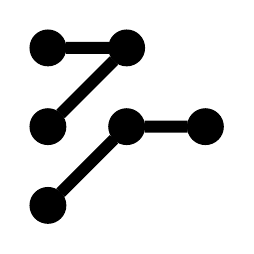
\begin{tikzpicture}
	\phantom{\draw (-0.25,-0.25) rectangle (2.25,2.25);}
	\node[draw,circle,fill=black,inner sep=0,outer sep=0,minimum size=3ex] (1) at (0,2) {};
	\node[draw,circle,fill=black,inner sep=0,outer sep=0,minimum size=3ex] (2) at (1,2) {};
	\node[draw,circle,fill=black,inner sep=0,outer sep=0,minimum size=3ex] (4) at (0,1) {};
	\node[draw,circle,fill=black,inner sep=0,outer sep=0,minimum size=3ex] (6) at (2,1) {};
	\node[draw,circle,fill=black,inner sep=0,outer sep=0,minimum size=3ex] (5) at (1,1) {};
	\node[draw,circle,fill=black,inner sep=0,outer sep=0,minimum size=3ex] (7) at (0,0) {};
	\draw[line width=1ex] (1) -- (2) -- (4);
	\draw[line width=1ex] (6) -- (5) -- (7);
\end{tikzpicture}
\newpage
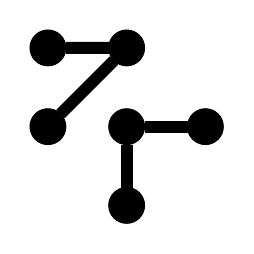
\begin{tikzpicture}
	\phantom{\draw (-0.25,-0.25) rectangle (2.25,2.25);}
	\node[draw,circle,fill=black,inner sep=0,outer sep=0,minimum size=3ex] (1) at (0,2) {};
	\node[draw,circle,fill=black,inner sep=0,outer sep=0,minimum size=3ex] (2) at (1,2) {};
	\node[draw,circle,fill=black,inner sep=0,outer sep=0,minimum size=3ex] (4) at (0,1) {};
	\node[draw,circle,fill=black,inner sep=0,outer sep=0,minimum size=3ex] (6) at (2,1) {};
	\node[draw,circle,fill=black,inner sep=0,outer sep=0,minimum size=3ex] (5) at (1,1) {};
	\node[draw,circle,fill=black,inner sep=0,outer sep=0,minimum size=3ex] (8) at (1,0) {};
	\draw[line width=1ex] (1) -- (2) -- (4);
	\draw[line width=1ex] (6) -- (5) -- (8);
\end{tikzpicture}
\newpage
\begin{tikzpicture}
	\phantom{\draw (-0.25,-0.25) rectangle (2.25,2.25);}
	\node[draw,circle,fill=black,inner sep=0,outer sep=0,minimum size=3ex] (1) at (0,2) {};
	\node[draw,circle,fill=black,inner sep=0,outer sep=0,minimum size=3ex] (2) at (1,2) {};
	\node[draw,circle,fill=black,inner sep=0,outer sep=0,minimum size=3ex] (4) at (0,1) {};
	\node[draw,circle,fill=black,inner sep=0,outer sep=0,minimum size=3ex] (6) at (2,1) {};
	\node[draw,circle,fill=black,inner sep=0,outer sep=0,minimum size=3ex] (5) at (1,1) {};
	\node[draw,circle,fill=black,inner sep=0,outer sep=0,minimum size=3ex] (9) at (2,0) {};
	\draw[line width=1ex] (1) -- (2) -- (4);
	\draw[line width=1ex] (6) -- (5) -- (9);
\end{tikzpicture}
\newpage
\begin{tikzpicture}
	\phantom{\draw (-0.25,-0.25) rectangle (2.25,2.25);}
	\node[draw,circle,fill=black,inner sep=0,outer sep=0,minimum size=3ex] (1) at (0,2) {};
	\node[draw,circle,fill=black,inner sep=0,outer sep=0,minimum size=3ex] (2) at (1,2) {};
	\node[draw,circle,fill=black,inner sep=0,outer sep=0,minimum size=3ex] (4) at (0,1) {};
	\node[draw,circle,fill=black,inner sep=0,outer sep=0,minimum size=3ex] (6) at (2,1) {};
	\node[draw,circle,fill=black,inner sep=0,outer sep=0,minimum size=3ex] (8) at (1,0) {};
	\node[draw,circle,fill=black,inner sep=0,outer sep=0,minimum size=3ex] (7) at (0,0) {};
	\draw[line width=1ex] (1) -- (2) -- (4);
	\draw[line width=1ex] (6) -- (8) -- (7);
\end{tikzpicture}
\newpage
\begin{tikzpicture}
	\phantom{\draw (-0.25,-0.25) rectangle (2.25,2.25);}
	\node[draw,circle,fill=black,inner sep=0,outer sep=0,minimum size=3ex] (1) at (0,2) {};
	\node[draw,circle,fill=black,inner sep=0,outer sep=0,minimum size=3ex] (2) at (1,2) {};
	\node[draw,circle,fill=black,inner sep=0,outer sep=0,minimum size=3ex] (4) at (0,1) {};
	\node[draw,circle,fill=black,inner sep=0,outer sep=0,minimum size=3ex] (6) at (2,1) {};
	\node[draw,circle,fill=black,inner sep=0,outer sep=0,minimum size=3ex] (8) at (1,0) {};
	\node[draw,circle,fill=black,inner sep=0,outer sep=0,minimum size=3ex] (9) at (2,0) {};
	\draw[line width=1ex] (1) -- (2) -- (4);
	\draw[line width=1ex] (6) -- (8) -- (9);
\end{tikzpicture}
\newpage
\begin{tikzpicture}
	\phantom{\draw (-0.25,-0.25) rectangle (2.25,2.25);}
	\node[draw,circle,fill=black,inner sep=0,outer sep=0,minimum size=3ex] (1) at (0,2) {};
	\node[draw,circle,fill=black,inner sep=0,outer sep=0,minimum size=3ex] (2) at (1,2) {};
	\node[draw,circle,fill=black,inner sep=0,outer sep=0,minimum size=3ex] (4) at (0,1) {};
	\node[draw,circle,fill=black,inner sep=0,outer sep=0,minimum size=3ex] (6) at (2,1) {};
	\node[draw,circle,fill=black,inner sep=0,outer sep=0,minimum size=3ex] (9) at (2,0) {};
	\node[draw,circle,fill=black,inner sep=0,outer sep=0,minimum size=3ex] (8) at (1,0) {};
	\draw[line width=1ex] (1) -- (2) -- (4);
	\draw[line width=1ex] (6) -- (9) -- (8);
\end{tikzpicture}
\newpage
\begin{tikzpicture}
	\phantom{\draw (-0.25,-0.25) rectangle (2.25,2.25);}
	\node[draw,circle,fill=black,inner sep=0,outer sep=0,minimum size=3ex] (1) at (0,2) {};
	\node[draw,circle,fill=black,inner sep=0,outer sep=0,minimum size=3ex] (2) at (1,2) {};
	\node[draw,circle,fill=black,inner sep=0,outer sep=0,minimum size=3ex] (4) at (0,1) {};
	\node[draw,circle,fill=black,inner sep=0,outer sep=0,minimum size=3ex] (7) at (0,0) {};
	\node[draw,circle,fill=black,inner sep=0,outer sep=0,minimum size=3ex] (5) at (1,1) {};
	\node[draw,circle,fill=black,inner sep=0,outer sep=0,minimum size=3ex] (8) at (1,0) {};
	\draw[line width=1ex] (1) -- (2) -- (4);
	\draw[line width=1ex] (7) -- (5) -- (8);
\end{tikzpicture}
\newpage
\begin{tikzpicture}
	\phantom{\draw (-0.25,-0.25) rectangle (2.25,2.25);}
	\node[draw,circle,fill=black,inner sep=0,outer sep=0,minimum size=3ex] (1) at (0,2) {};
	\node[draw,circle,fill=black,inner sep=0,outer sep=0,minimum size=3ex] (2) at (1,2) {};
	\node[draw,circle,fill=black,inner sep=0,outer sep=0,minimum size=3ex] (4) at (0,1) {};
	\node[draw,circle,fill=black,inner sep=0,outer sep=0,minimum size=3ex] (7) at (0,0) {};
	\node[draw,circle,fill=black,inner sep=0,outer sep=0,minimum size=3ex] (5) at (1,1) {};
	\node[draw,circle,fill=black,inner sep=0,outer sep=0,minimum size=3ex] (9) at (2,0) {};
	\draw[line width=1ex] (1) -- (2) -- (4);
	\draw[line width=1ex] (7) -- (5) -- (9);
\end{tikzpicture}
\newpage
\begin{tikzpicture}
	\phantom{\draw (-0.25,-0.25) rectangle (2.25,2.25);}
	\node[draw,circle,fill=black,inner sep=0,outer sep=0,minimum size=3ex] (1) at (0,2) {};
	\node[draw,circle,fill=black,inner sep=0,outer sep=0,minimum size=3ex] (2) at (1,2) {};
	\node[draw,circle,fill=black,inner sep=0,outer sep=0,minimum size=3ex] (4) at (0,1) {};
	\node[draw,circle,fill=black,inner sep=0,outer sep=0,minimum size=3ex] (7) at (0,0) {};
	\node[draw,circle,fill=black,inner sep=0,outer sep=0,minimum size=3ex] (8) at (1,0) {};
	\node[draw,circle,fill=black,inner sep=0,outer sep=0,minimum size=3ex] (9) at (2,0) {};
	\draw[line width=1ex] (1) -- (2) -- (4);
	\draw[line width=1ex] (7) -- (8) -- (9);
\end{tikzpicture}
\newpage
\begin{tikzpicture}
	\phantom{\draw (-0.25,-0.25) rectangle (2.25,2.25);}
	\node[draw,circle,fill=black,inner sep=0,outer sep=0,minimum size=3ex] (1) at (0,2) {};
	\node[draw,circle,fill=black,inner sep=0,outer sep=0,minimum size=3ex] (2) at (1,2) {};
	\node[draw,circle,fill=black,inner sep=0,outer sep=0,minimum size=3ex] (4) at (0,1) {};
	\node[draw,circle,fill=black,inner sep=0,outer sep=0,minimum size=3ex] (8) at (1,0) {};
	\node[draw,circle,fill=black,inner sep=0,outer sep=0,minimum size=3ex] (5) at (1,1) {};
	\node[draw,circle,fill=black,inner sep=0,outer sep=0,minimum size=3ex] (9) at (2,0) {};
	\draw[line width=1ex] (1) -- (2) -- (4);
	\draw[line width=1ex] (8) -- (5) -- (9);
\end{tikzpicture}
\newpage
\begin{tikzpicture}
	\phantom{\draw (-0.25,-0.25) rectangle (2.25,2.25);}
	\node[draw,circle,fill=black,inner sep=0,outer sep=0,minimum size=3ex] (1) at (0,2) {};
	\node[draw,circle,fill=black,inner sep=0,outer sep=0,minimum size=3ex] (2) at (1,2) {};
	\node[draw,circle,fill=black,inner sep=0,outer sep=0,minimum size=3ex] (4) at (0,1) {};
	\node[draw,circle,fill=black,inner sep=0,outer sep=0,minimum size=3ex] (8) at (1,0) {};
	\node[draw,circle,fill=black,inner sep=0,outer sep=0,minimum size=3ex] (6) at (2,1) {};
	\node[draw,circle,fill=black,inner sep=0,outer sep=0,minimum size=3ex] (9) at (2,0) {};
	\draw[line width=1ex] (1) -- (2) -- (4);
	\draw[line width=1ex] (8) -- (6) -- (9);
\end{tikzpicture}
\newpage
\begin{tikzpicture}
	\phantom{\draw (-0.25,-0.25) rectangle (2.25,2.25);}
	\node[draw,circle,fill=black,inner sep=0,outer sep=0,minimum size=3ex] (1) at (0,2) {};
	\node[draw,circle,fill=black,inner sep=0,outer sep=0,minimum size=3ex] (2) at (1,2) {};
	\node[draw,circle,fill=black,inner sep=0,outer sep=0,minimum size=3ex] (5) at (1,1) {};
	\node[draw,circle,fill=black,inner sep=0,outer sep=0,minimum size=3ex] (3) at (2,2) {};
	\node[draw,circle,fill=black,inner sep=0,outer sep=0,minimum size=3ex] (6) at (2,1) {};
	\node[draw,circle,fill=black,inner sep=0,outer sep=0,minimum size=3ex] (8) at (1,0) {};
	\draw[line width=1ex] (1) -- (2) -- (5);
	\draw[line width=1ex] (3) -- (6) -- (8);
\end{tikzpicture}
\newpage
\begin{tikzpicture}
	\phantom{\draw (-0.25,-0.25) rectangle (2.25,2.25);}
	\node[draw,circle,fill=black,inner sep=0,outer sep=0,minimum size=3ex] (1) at (0,2) {};
	\node[draw,circle,fill=black,inner sep=0,outer sep=0,minimum size=3ex] (2) at (1,2) {};
	\node[draw,circle,fill=black,inner sep=0,outer sep=0,minimum size=3ex] (5) at (1,1) {};
	\node[draw,circle,fill=black,inner sep=0,outer sep=0,minimum size=3ex] (3) at (2,2) {};
	\node[draw,circle,fill=black,inner sep=0,outer sep=0,minimum size=3ex] (6) at (2,1) {};
	\node[draw,circle,fill=black,inner sep=0,outer sep=0,minimum size=3ex] (9) at (2,0) {};
	\draw[line width=1ex] (1) -- (2) -- (5);
	\draw[line width=1ex] (3) -- (6) -- (9);
\end{tikzpicture}
\newpage
\begin{tikzpicture}
	\phantom{\draw (-0.25,-0.25) rectangle (2.25,2.25);}
	\node[draw,circle,fill=black,inner sep=0,outer sep=0,minimum size=3ex] (1) at (0,2) {};
	\node[draw,circle,fill=black,inner sep=0,outer sep=0,minimum size=3ex] (2) at (1,2) {};
	\node[draw,circle,fill=black,inner sep=0,outer sep=0,minimum size=3ex] (5) at (1,1) {};
	\node[draw,circle,fill=black,inner sep=0,outer sep=0,minimum size=3ex] (4) at (0,1) {};
	\node[draw,circle,fill=black,inner sep=0,outer sep=0,minimum size=3ex] (7) at (0,0) {};
	\node[draw,circle,fill=black,inner sep=0,outer sep=0,minimum size=3ex] (8) at (1,0) {};
	\draw[line width=1ex] (1) -- (2) -- (5);
	\draw[line width=1ex] (4) -- (7) -- (8);
\end{tikzpicture}
\newpage
\begin{tikzpicture}
	\phantom{\draw (-0.25,-0.25) rectangle (2.25,2.25);}
	\node[draw,circle,fill=black,inner sep=0,outer sep=0,minimum size=3ex] (1) at (0,2) {};
	\node[draw,circle,fill=black,inner sep=0,outer sep=0,minimum size=3ex] (2) at (1,2) {};
	\node[draw,circle,fill=black,inner sep=0,outer sep=0,minimum size=3ex] (5) at (1,1) {};
	\node[draw,circle,fill=black,inner sep=0,outer sep=0,minimum size=3ex] (4) at (0,1) {};
	\node[draw,circle,fill=black,inner sep=0,outer sep=0,minimum size=3ex] (8) at (1,0) {};
	\node[draw,circle,fill=black,inner sep=0,outer sep=0,minimum size=3ex] (6) at (2,1) {};
	\draw[line width=1ex] (1) -- (2) -- (5);
	\draw[line width=1ex] (4) -- (8) -- (6);
\end{tikzpicture}
\newpage
\begin{tikzpicture}
	\phantom{\draw (-0.25,-0.25) rectangle (2.25,2.25);}
	\node[draw,circle,fill=black,inner sep=0,outer sep=0,minimum size=3ex] (1) at (0,2) {};
	\node[draw,circle,fill=black,inner sep=0,outer sep=0,minimum size=3ex] (2) at (1,2) {};
	\node[draw,circle,fill=black,inner sep=0,outer sep=0,minimum size=3ex] (5) at (1,1) {};
	\node[draw,circle,fill=black,inner sep=0,outer sep=0,minimum size=3ex] (4) at (0,1) {};
	\node[draw,circle,fill=black,inner sep=0,outer sep=0,minimum size=3ex] (8) at (1,0) {};
	\node[draw,circle,fill=black,inner sep=0,outer sep=0,minimum size=3ex] (7) at (0,0) {};
	\draw[line width=1ex] (1) -- (2) -- (5);
	\draw[line width=1ex] (4) -- (8) -- (7);
\end{tikzpicture}
\newpage
\begin{tikzpicture}
	\phantom{\draw (-0.25,-0.25) rectangle (2.25,2.25);}
	\node[draw,circle,fill=black,inner sep=0,outer sep=0,minimum size=3ex] (1) at (0,2) {};
	\node[draw,circle,fill=black,inner sep=0,outer sep=0,minimum size=3ex] (2) at (1,2) {};
	\node[draw,circle,fill=black,inner sep=0,outer sep=0,minimum size=3ex] (5) at (1,1) {};
	\node[draw,circle,fill=black,inner sep=0,outer sep=0,minimum size=3ex] (4) at (0,1) {};
	\node[draw,circle,fill=black,inner sep=0,outer sep=0,minimum size=3ex] (8) at (1,0) {};
	\node[draw,circle,fill=black,inner sep=0,outer sep=0,minimum size=3ex] (9) at (2,0) {};
	\draw[line width=1ex] (1) -- (2) -- (5);
	\draw[line width=1ex] (4) -- (8) -- (9);
\end{tikzpicture}
\newpage
\begin{tikzpicture}
	\phantom{\draw (-0.25,-0.25) rectangle (2.25,2.25);}
	\node[draw,circle,fill=black,inner sep=0,outer sep=0,minimum size=3ex] (1) at (0,2) {};
	\node[draw,circle,fill=black,inner sep=0,outer sep=0,minimum size=3ex] (2) at (1,2) {};
	\node[draw,circle,fill=black,inner sep=0,outer sep=0,minimum size=3ex] (5) at (1,1) {};
	\node[draw,circle,fill=black,inner sep=0,outer sep=0,minimum size=3ex] (6) at (2,1) {};
	\node[draw,circle,fill=black,inner sep=0,outer sep=0,minimum size=3ex] (8) at (1,0) {};
	\node[draw,circle,fill=black,inner sep=0,outer sep=0,minimum size=3ex] (7) at (0,0) {};
	\draw[line width=1ex] (1) -- (2) -- (5);
	\draw[line width=1ex] (6) -- (8) -- (7);
\end{tikzpicture}
\newpage
\begin{tikzpicture}
	\phantom{\draw (-0.25,-0.25) rectangle (2.25,2.25);}
	\node[draw,circle,fill=black,inner sep=0,outer sep=0,minimum size=3ex] (1) at (0,2) {};
	\node[draw,circle,fill=black,inner sep=0,outer sep=0,minimum size=3ex] (2) at (1,2) {};
	\node[draw,circle,fill=black,inner sep=0,outer sep=0,minimum size=3ex] (5) at (1,1) {};
	\node[draw,circle,fill=black,inner sep=0,outer sep=0,minimum size=3ex] (6) at (2,1) {};
	\node[draw,circle,fill=black,inner sep=0,outer sep=0,minimum size=3ex] (8) at (1,0) {};
	\node[draw,circle,fill=black,inner sep=0,outer sep=0,minimum size=3ex] (9) at (2,0) {};
	\draw[line width=1ex] (1) -- (2) -- (5);
	\draw[line width=1ex] (6) -- (8) -- (9);
\end{tikzpicture}
\newpage
\begin{tikzpicture}
	\phantom{\draw (-0.25,-0.25) rectangle (2.25,2.25);}
	\node[draw,circle,fill=black,inner sep=0,outer sep=0,minimum size=3ex] (1) at (0,2) {};
	\node[draw,circle,fill=black,inner sep=0,outer sep=0,minimum size=3ex] (2) at (1,2) {};
	\node[draw,circle,fill=black,inner sep=0,outer sep=0,minimum size=3ex] (5) at (1,1) {};
	\node[draw,circle,fill=black,inner sep=0,outer sep=0,minimum size=3ex] (6) at (2,1) {};
	\node[draw,circle,fill=black,inner sep=0,outer sep=0,minimum size=3ex] (9) at (2,0) {};
	\node[draw,circle,fill=black,inner sep=0,outer sep=0,minimum size=3ex] (8) at (1,0) {};
	\draw[line width=1ex] (1) -- (2) -- (5);
	\draw[line width=1ex] (6) -- (9) -- (8);
\end{tikzpicture}
\newpage
\begin{tikzpicture}
	\phantom{\draw (-0.25,-0.25) rectangle (2.25,2.25);}
	\node[draw,circle,fill=black,inner sep=0,outer sep=0,minimum size=3ex] (1) at (0,2) {};
	\node[draw,circle,fill=black,inner sep=0,outer sep=0,minimum size=3ex] (2) at (1,2) {};
	\node[draw,circle,fill=black,inner sep=0,outer sep=0,minimum size=3ex] (5) at (1,1) {};
	\node[draw,circle,fill=black,inner sep=0,outer sep=0,minimum size=3ex] (7) at (0,0) {};
	\node[draw,circle,fill=black,inner sep=0,outer sep=0,minimum size=3ex] (4) at (0,1) {};
	\node[draw,circle,fill=black,inner sep=0,outer sep=0,minimum size=3ex] (8) at (1,0) {};
	\draw[line width=1ex] (1) -- (2) -- (5);
	\draw[line width=1ex] (7) -- (4) -- (8);
\end{tikzpicture}
\newpage
\begin{tikzpicture}
	\phantom{\draw (-0.25,-0.25) rectangle (2.25,2.25);}
	\node[draw,circle,fill=black,inner sep=0,outer sep=0,minimum size=3ex] (1) at (0,2) {};
	\node[draw,circle,fill=black,inner sep=0,outer sep=0,minimum size=3ex] (2) at (1,2) {};
	\node[draw,circle,fill=black,inner sep=0,outer sep=0,minimum size=3ex] (5) at (1,1) {};
	\node[draw,circle,fill=black,inner sep=0,outer sep=0,minimum size=3ex] (7) at (0,0) {};
	\node[draw,circle,fill=black,inner sep=0,outer sep=0,minimum size=3ex] (8) at (1,0) {};
	\node[draw,circle,fill=black,inner sep=0,outer sep=0,minimum size=3ex] (9) at (2,0) {};
	\draw[line width=1ex] (1) -- (2) -- (5);
	\draw[line width=1ex] (7) -- (8) -- (9);
\end{tikzpicture}
\newpage
\begin{tikzpicture}
	\phantom{\draw (-0.25,-0.25) rectangle (2.25,2.25);}
	\node[draw,circle,fill=black,inner sep=0,outer sep=0,minimum size=3ex] (1) at (0,2) {};
	\node[draw,circle,fill=black,inner sep=0,outer sep=0,minimum size=3ex] (2) at (1,2) {};
	\node[draw,circle,fill=black,inner sep=0,outer sep=0,minimum size=3ex] (5) at (1,1) {};
	\node[draw,circle,fill=black,inner sep=0,outer sep=0,minimum size=3ex] (8) at (1,0) {};
	\node[draw,circle,fill=black,inner sep=0,outer sep=0,minimum size=3ex] (6) at (2,1) {};
	\node[draw,circle,fill=black,inner sep=0,outer sep=0,minimum size=3ex] (9) at (2,0) {};
	\draw[line width=1ex] (1) -- (2) -- (5);
	\draw[line width=1ex] (8) -- (6) -- (9);
\end{tikzpicture}
\newpage
\begin{tikzpicture}
	\phantom{\draw (-0.25,-0.25) rectangle (2.25,2.25);}
	\node[draw,circle,fill=black,inner sep=0,outer sep=0,minimum size=3ex] (1) at (0,2) {};
	\node[draw,circle,fill=black,inner sep=0,outer sep=0,minimum size=3ex] (2) at (1,2) {};
	\node[draw,circle,fill=black,inner sep=0,outer sep=0,minimum size=3ex] (6) at (2,1) {};
	\node[draw,circle,fill=black,inner sep=0,outer sep=0,minimum size=3ex] (4) at (0,1) {};
	\node[draw,circle,fill=black,inner sep=0,outer sep=0,minimum size=3ex] (5) at (1,1) {};
	\node[draw,circle,fill=black,inner sep=0,outer sep=0,minimum size=3ex] (7) at (0,0) {};
	\draw[line width=1ex] (1) -- (2) -- (6);
	\draw[line width=1ex] (4) -- (5) -- (7);
\end{tikzpicture}
\newpage
\begin{tikzpicture}
	\phantom{\draw (-0.25,-0.25) rectangle (2.25,2.25);}
	\node[draw,circle,fill=black,inner sep=0,outer sep=0,minimum size=3ex] (1) at (0,2) {};
	\node[draw,circle,fill=black,inner sep=0,outer sep=0,minimum size=3ex] (2) at (1,2) {};
	\node[draw,circle,fill=black,inner sep=0,outer sep=0,minimum size=3ex] (6) at (2,1) {};
	\node[draw,circle,fill=black,inner sep=0,outer sep=0,minimum size=3ex] (4) at (0,1) {};
	\node[draw,circle,fill=black,inner sep=0,outer sep=0,minimum size=3ex] (5) at (1,1) {};
	\node[draw,circle,fill=black,inner sep=0,outer sep=0,minimum size=3ex] (8) at (1,0) {};
	\draw[line width=1ex] (1) -- (2) -- (6);
	\draw[line width=1ex] (4) -- (5) -- (8);
\end{tikzpicture}
\newpage
\begin{tikzpicture}
	\phantom{\draw (-0.25,-0.25) rectangle (2.25,2.25);}
	\node[draw,circle,fill=black,inner sep=0,outer sep=0,minimum size=3ex] (1) at (0,2) {};
	\node[draw,circle,fill=black,inner sep=0,outer sep=0,minimum size=3ex] (2) at (1,2) {};
	\node[draw,circle,fill=black,inner sep=0,outer sep=0,minimum size=3ex] (6) at (2,1) {};
	\node[draw,circle,fill=black,inner sep=0,outer sep=0,minimum size=3ex] (4) at (0,1) {};
	\node[draw,circle,fill=black,inner sep=0,outer sep=0,minimum size=3ex] (5) at (1,1) {};
	\node[draw,circle,fill=black,inner sep=0,outer sep=0,minimum size=3ex] (9) at (2,0) {};
	\draw[line width=1ex] (1) -- (2) -- (6);
	\draw[line width=1ex] (4) -- (5) -- (9);
\end{tikzpicture}
\newpage
\begin{tikzpicture}
	\phantom{\draw (-0.25,-0.25) rectangle (2.25,2.25);}
	\node[draw,circle,fill=black,inner sep=0,outer sep=0,minimum size=3ex] (1) at (0,2) {};
	\node[draw,circle,fill=black,inner sep=0,outer sep=0,minimum size=3ex] (2) at (1,2) {};
	\node[draw,circle,fill=black,inner sep=0,outer sep=0,minimum size=3ex] (6) at (2,1) {};
	\node[draw,circle,fill=black,inner sep=0,outer sep=0,minimum size=3ex] (4) at (0,1) {};
	\node[draw,circle,fill=black,inner sep=0,outer sep=0,minimum size=3ex] (7) at (0,0) {};
	\node[draw,circle,fill=black,inner sep=0,outer sep=0,minimum size=3ex] (5) at (1,1) {};
	\draw[line width=1ex] (1) -- (2) -- (6);
	\draw[line width=1ex] (4) -- (7) -- (5);
\end{tikzpicture}
\newpage
\begin{tikzpicture}
	\phantom{\draw (-0.25,-0.25) rectangle (2.25,2.25);}
	\node[draw,circle,fill=black,inner sep=0,outer sep=0,minimum size=3ex] (1) at (0,2) {};
	\node[draw,circle,fill=black,inner sep=0,outer sep=0,minimum size=3ex] (2) at (1,2) {};
	\node[draw,circle,fill=black,inner sep=0,outer sep=0,minimum size=3ex] (6) at (2,1) {};
	\node[draw,circle,fill=black,inner sep=0,outer sep=0,minimum size=3ex] (4) at (0,1) {};
	\node[draw,circle,fill=black,inner sep=0,outer sep=0,minimum size=3ex] (7) at (0,0) {};
	\node[draw,circle,fill=black,inner sep=0,outer sep=0,minimum size=3ex] (8) at (1,0) {};
	\draw[line width=1ex] (1) -- (2) -- (6);
	\draw[line width=1ex] (4) -- (7) -- (8);
\end{tikzpicture}
\newpage
\begin{tikzpicture}
	\phantom{\draw (-0.25,-0.25) rectangle (2.25,2.25);}
	\node[draw,circle,fill=black,inner sep=0,outer sep=0,minimum size=3ex] (1) at (0,2) {};
	\node[draw,circle,fill=black,inner sep=0,outer sep=0,minimum size=3ex] (2) at (1,2) {};
	\node[draw,circle,fill=black,inner sep=0,outer sep=0,minimum size=3ex] (6) at (2,1) {};
	\node[draw,circle,fill=black,inner sep=0,outer sep=0,minimum size=3ex] (4) at (0,1) {};
	\node[draw,circle,fill=black,inner sep=0,outer sep=0,minimum size=3ex] (8) at (1,0) {};
	\node[draw,circle,fill=black,inner sep=0,outer sep=0,minimum size=3ex] (5) at (1,1) {};
	\draw[line width=1ex] (1) -- (2) -- (6);
	\draw[line width=1ex] (4) -- (8) -- (5);
\end{tikzpicture}
\newpage
\begin{tikzpicture}
	\phantom{\draw (-0.25,-0.25) rectangle (2.25,2.25);}
	\node[draw,circle,fill=black,inner sep=0,outer sep=0,minimum size=3ex] (1) at (0,2) {};
	\node[draw,circle,fill=black,inner sep=0,outer sep=0,minimum size=3ex] (2) at (1,2) {};
	\node[draw,circle,fill=black,inner sep=0,outer sep=0,minimum size=3ex] (6) at (2,1) {};
	\node[draw,circle,fill=black,inner sep=0,outer sep=0,minimum size=3ex] (4) at (0,1) {};
	\node[draw,circle,fill=black,inner sep=0,outer sep=0,minimum size=3ex] (8) at (1,0) {};
	\node[draw,circle,fill=black,inner sep=0,outer sep=0,minimum size=3ex] (7) at (0,0) {};
	\draw[line width=1ex] (1) -- (2) -- (6);
	\draw[line width=1ex] (4) -- (8) -- (7);
\end{tikzpicture}
\newpage
\begin{tikzpicture}
	\phantom{\draw (-0.25,-0.25) rectangle (2.25,2.25);}
	\node[draw,circle,fill=black,inner sep=0,outer sep=0,minimum size=3ex] (1) at (0,2) {};
	\node[draw,circle,fill=black,inner sep=0,outer sep=0,minimum size=3ex] (2) at (1,2) {};
	\node[draw,circle,fill=black,inner sep=0,outer sep=0,minimum size=3ex] (6) at (2,1) {};
	\node[draw,circle,fill=black,inner sep=0,outer sep=0,minimum size=3ex] (4) at (0,1) {};
	\node[draw,circle,fill=black,inner sep=0,outer sep=0,minimum size=3ex] (8) at (1,0) {};
	\node[draw,circle,fill=black,inner sep=0,outer sep=0,minimum size=3ex] (9) at (2,0) {};
	\draw[line width=1ex] (1) -- (2) -- (6);
	\draw[line width=1ex] (4) -- (8) -- (9);
\end{tikzpicture}
\newpage
\begin{tikzpicture}
	\phantom{\draw (-0.25,-0.25) rectangle (2.25,2.25);}
	\node[draw,circle,fill=black,inner sep=0,outer sep=0,minimum size=3ex] (1) at (0,2) {};
	\node[draw,circle,fill=black,inner sep=0,outer sep=0,minimum size=3ex] (2) at (1,2) {};
	\node[draw,circle,fill=black,inner sep=0,outer sep=0,minimum size=3ex] (6) at (2,1) {};
	\node[draw,circle,fill=black,inner sep=0,outer sep=0,minimum size=3ex] (5) at (1,1) {};
	\node[draw,circle,fill=black,inner sep=0,outer sep=0,minimum size=3ex] (4) at (0,1) {};
	\node[draw,circle,fill=black,inner sep=0,outer sep=0,minimum size=3ex] (7) at (0,0) {};
	\draw[line width=1ex] (1) -- (2) -- (6);
	\draw[line width=1ex] (5) -- (4) -- (7);
\end{tikzpicture}
\newpage
\begin{tikzpicture}
	\phantom{\draw (-0.25,-0.25) rectangle (2.25,2.25);}
	\node[draw,circle,fill=black,inner sep=0,outer sep=0,minimum size=3ex] (1) at (0,2) {};
	\node[draw,circle,fill=black,inner sep=0,outer sep=0,minimum size=3ex] (2) at (1,2) {};
	\node[draw,circle,fill=black,inner sep=0,outer sep=0,minimum size=3ex] (6) at (2,1) {};
	\node[draw,circle,fill=black,inner sep=0,outer sep=0,minimum size=3ex] (5) at (1,1) {};
	\node[draw,circle,fill=black,inner sep=0,outer sep=0,minimum size=3ex] (4) at (0,1) {};
	\node[draw,circle,fill=black,inner sep=0,outer sep=0,minimum size=3ex] (8) at (1,0) {};
	\draw[line width=1ex] (1) -- (2) -- (6);
	\draw[line width=1ex] (5) -- (4) -- (8);
\end{tikzpicture}
\newpage
\begin{tikzpicture}
	\phantom{\draw (-0.25,-0.25) rectangle (2.25,2.25);}
	\node[draw,circle,fill=black,inner sep=0,outer sep=0,minimum size=3ex] (1) at (0,2) {};
	\node[draw,circle,fill=black,inner sep=0,outer sep=0,minimum size=3ex] (2) at (1,2) {};
	\node[draw,circle,fill=black,inner sep=0,outer sep=0,minimum size=3ex] (6) at (2,1) {};
	\node[draw,circle,fill=black,inner sep=0,outer sep=0,minimum size=3ex] (5) at (1,1) {};
	\node[draw,circle,fill=black,inner sep=0,outer sep=0,minimum size=3ex] (7) at (0,0) {};
	\node[draw,circle,fill=black,inner sep=0,outer sep=0,minimum size=3ex] (8) at (1,0) {};
	\draw[line width=1ex] (1) -- (2) -- (6);
	\draw[line width=1ex] (5) -- (7) -- (8);
\end{tikzpicture}
\newpage
\begin{tikzpicture}
	\phantom{\draw (-0.25,-0.25) rectangle (2.25,2.25);}
	\node[draw,circle,fill=black,inner sep=0,outer sep=0,minimum size=3ex] (1) at (0,2) {};
	\node[draw,circle,fill=black,inner sep=0,outer sep=0,minimum size=3ex] (2) at (1,2) {};
	\node[draw,circle,fill=black,inner sep=0,outer sep=0,minimum size=3ex] (6) at (2,1) {};
	\node[draw,circle,fill=black,inner sep=0,outer sep=0,minimum size=3ex] (5) at (1,1) {};
	\node[draw,circle,fill=black,inner sep=0,outer sep=0,minimum size=3ex] (8) at (1,0) {};
	\node[draw,circle,fill=black,inner sep=0,outer sep=0,minimum size=3ex] (7) at (0,0) {};
	\draw[line width=1ex] (1) -- (2) -- (6);
	\draw[line width=1ex] (5) -- (8) -- (7);
\end{tikzpicture}
\newpage
\begin{tikzpicture}
	\phantom{\draw (-0.25,-0.25) rectangle (2.25,2.25);}
	\node[draw,circle,fill=black,inner sep=0,outer sep=0,minimum size=3ex] (1) at (0,2) {};
	\node[draw,circle,fill=black,inner sep=0,outer sep=0,minimum size=3ex] (2) at (1,2) {};
	\node[draw,circle,fill=black,inner sep=0,outer sep=0,minimum size=3ex] (6) at (2,1) {};
	\node[draw,circle,fill=black,inner sep=0,outer sep=0,minimum size=3ex] (5) at (1,1) {};
	\node[draw,circle,fill=black,inner sep=0,outer sep=0,minimum size=3ex] (8) at (1,0) {};
	\node[draw,circle,fill=black,inner sep=0,outer sep=0,minimum size=3ex] (9) at (2,0) {};
	\draw[line width=1ex] (1) -- (2) -- (6);
	\draw[line width=1ex] (5) -- (8) -- (9);
\end{tikzpicture}
\newpage
\begin{tikzpicture}
	\phantom{\draw (-0.25,-0.25) rectangle (2.25,2.25);}
	\node[draw,circle,fill=black,inner sep=0,outer sep=0,minimum size=3ex] (1) at (0,2) {};
	\node[draw,circle,fill=black,inner sep=0,outer sep=0,minimum size=3ex] (2) at (1,2) {};
	\node[draw,circle,fill=black,inner sep=0,outer sep=0,minimum size=3ex] (6) at (2,1) {};
	\node[draw,circle,fill=black,inner sep=0,outer sep=0,minimum size=3ex] (5) at (1,1) {};
	\node[draw,circle,fill=black,inner sep=0,outer sep=0,minimum size=3ex] (9) at (2,0) {};
	\node[draw,circle,fill=black,inner sep=0,outer sep=0,minimum size=3ex] (8) at (1,0) {};
	\draw[line width=1ex] (1) -- (2) -- (6);
	\draw[line width=1ex] (5) -- (9) -- (8);
\end{tikzpicture}
\newpage
\begin{tikzpicture}
	\phantom{\draw (-0.25,-0.25) rectangle (2.25,2.25);}
	\node[draw,circle,fill=black,inner sep=0,outer sep=0,minimum size=3ex] (1) at (0,2) {};
	\node[draw,circle,fill=black,inner sep=0,outer sep=0,minimum size=3ex] (2) at (1,2) {};
	\node[draw,circle,fill=black,inner sep=0,outer sep=0,minimum size=3ex] (6) at (2,1) {};
	\node[draw,circle,fill=black,inner sep=0,outer sep=0,minimum size=3ex] (7) at (0,0) {};
	\node[draw,circle,fill=black,inner sep=0,outer sep=0,minimum size=3ex] (4) at (0,1) {};
	\node[draw,circle,fill=black,inner sep=0,outer sep=0,minimum size=3ex] (8) at (1,0) {};
	\draw[line width=1ex] (1) -- (2) -- (6);
	\draw[line width=1ex] (7) -- (4) -- (8);
\end{tikzpicture}
\newpage
\begin{tikzpicture}
	\phantom{\draw (-0.25,-0.25) rectangle (2.25,2.25);}
	\node[draw,circle,fill=black,inner sep=0,outer sep=0,minimum size=3ex] (1) at (0,2) {};
	\node[draw,circle,fill=black,inner sep=0,outer sep=0,minimum size=3ex] (2) at (1,2) {};
	\node[draw,circle,fill=black,inner sep=0,outer sep=0,minimum size=3ex] (6) at (2,1) {};
	\node[draw,circle,fill=black,inner sep=0,outer sep=0,minimum size=3ex] (7) at (0,0) {};
	\node[draw,circle,fill=black,inner sep=0,outer sep=0,minimum size=3ex] (5) at (1,1) {};
	\node[draw,circle,fill=black,inner sep=0,outer sep=0,minimum size=3ex] (8) at (1,0) {};
	\draw[line width=1ex] (1) -- (2) -- (6);
	\draw[line width=1ex] (7) -- (5) -- (8);
\end{tikzpicture}
\newpage
\begin{tikzpicture}
	\phantom{\draw (-0.25,-0.25) rectangle (2.25,2.25);}
	\node[draw,circle,fill=black,inner sep=0,outer sep=0,minimum size=3ex] (1) at (0,2) {};
	\node[draw,circle,fill=black,inner sep=0,outer sep=0,minimum size=3ex] (2) at (1,2) {};
	\node[draw,circle,fill=black,inner sep=0,outer sep=0,minimum size=3ex] (6) at (2,1) {};
	\node[draw,circle,fill=black,inner sep=0,outer sep=0,minimum size=3ex] (7) at (0,0) {};
	\node[draw,circle,fill=black,inner sep=0,outer sep=0,minimum size=3ex] (5) at (1,1) {};
	\node[draw,circle,fill=black,inner sep=0,outer sep=0,minimum size=3ex] (9) at (2,0) {};
	\draw[line width=1ex] (1) -- (2) -- (6);
	\draw[line width=1ex] (7) -- (5) -- (9);
\end{tikzpicture}
\newpage
\begin{tikzpicture}
	\phantom{\draw (-0.25,-0.25) rectangle (2.25,2.25);}
	\node[draw,circle,fill=black,inner sep=0,outer sep=0,minimum size=3ex] (1) at (0,2) {};
	\node[draw,circle,fill=black,inner sep=0,outer sep=0,minimum size=3ex] (2) at (1,2) {};
	\node[draw,circle,fill=black,inner sep=0,outer sep=0,minimum size=3ex] (6) at (2,1) {};
	\node[draw,circle,fill=black,inner sep=0,outer sep=0,minimum size=3ex] (7) at (0,0) {};
	\node[draw,circle,fill=black,inner sep=0,outer sep=0,minimum size=3ex] (8) at (1,0) {};
	\node[draw,circle,fill=black,inner sep=0,outer sep=0,minimum size=3ex] (9) at (2,0) {};
	\draw[line width=1ex] (1) -- (2) -- (6);
	\draw[line width=1ex] (7) -- (8) -- (9);
\end{tikzpicture}
\newpage
\begin{tikzpicture}
	\phantom{\draw (-0.25,-0.25) rectangle (2.25,2.25);}
	\node[draw,circle,fill=black,inner sep=0,outer sep=0,minimum size=3ex] (1) at (0,2) {};
	\node[draw,circle,fill=black,inner sep=0,outer sep=0,minimum size=3ex] (2) at (1,2) {};
	\node[draw,circle,fill=black,inner sep=0,outer sep=0,minimum size=3ex] (6) at (2,1) {};
	\node[draw,circle,fill=black,inner sep=0,outer sep=0,minimum size=3ex] (8) at (1,0) {};
	\node[draw,circle,fill=black,inner sep=0,outer sep=0,minimum size=3ex] (5) at (1,1) {};
	\node[draw,circle,fill=black,inner sep=0,outer sep=0,minimum size=3ex] (9) at (2,0) {};
	\draw[line width=1ex] (1) -- (2) -- (6);
	\draw[line width=1ex] (8) -- (5) -- (9);
\end{tikzpicture}
\newpage
\begin{tikzpicture}
	\phantom{\draw (-0.25,-0.25) rectangle (2.25,2.25);}
	\node[draw,circle,fill=black,inner sep=0,outer sep=0,minimum size=3ex] (1) at (0,2) {};
	\node[draw,circle,fill=black,inner sep=0,outer sep=0,minimum size=3ex] (4) at (0,1) {};
	\node[draw,circle,fill=black,inner sep=0,outer sep=0,minimum size=3ex] (2) at (1,2) {};
	\node[draw,circle,fill=black,inner sep=0,outer sep=0,minimum size=3ex] (3) at (2,2) {};
	\node[draw,circle,fill=black,inner sep=0,outer sep=0,minimum size=3ex] (5) at (1,1) {};
	\node[draw,circle,fill=black,inner sep=0,outer sep=0,minimum size=3ex] (6) at (2,1) {};
	\draw[line width=1ex] (1) -- (4) -- (2);
	\draw[line width=1ex] (3) -- (5) -- (6);
\end{tikzpicture}
\newpage
\begin{tikzpicture}
	\phantom{\draw (-0.25,-0.25) rectangle (2.25,2.25);}
	\node[draw,circle,fill=black,inner sep=0,outer sep=0,minimum size=3ex] (1) at (0,2) {};
	\node[draw,circle,fill=black,inner sep=0,outer sep=0,minimum size=3ex] (4) at (0,1) {};
	\node[draw,circle,fill=black,inner sep=0,outer sep=0,minimum size=3ex] (2) at (1,2) {};
	\node[draw,circle,fill=black,inner sep=0,outer sep=0,minimum size=3ex] (3) at (2,2) {};
	\node[draw,circle,fill=black,inner sep=0,outer sep=0,minimum size=3ex] (5) at (1,1) {};
	\node[draw,circle,fill=black,inner sep=0,outer sep=0,minimum size=3ex] (7) at (0,0) {};
	\draw[line width=1ex] (1) -- (4) -- (2);
	\draw[line width=1ex] (3) -- (5) -- (7);
\end{tikzpicture}
\newpage
\begin{tikzpicture}
	\phantom{\draw (-0.25,-0.25) rectangle (2.25,2.25);}
	\node[draw,circle,fill=black,inner sep=0,outer sep=0,minimum size=3ex] (1) at (0,2) {};
	\node[draw,circle,fill=black,inner sep=0,outer sep=0,minimum size=3ex] (4) at (0,1) {};
	\node[draw,circle,fill=black,inner sep=0,outer sep=0,minimum size=3ex] (2) at (1,2) {};
	\node[draw,circle,fill=black,inner sep=0,outer sep=0,minimum size=3ex] (3) at (2,2) {};
	\node[draw,circle,fill=black,inner sep=0,outer sep=0,minimum size=3ex] (5) at (1,1) {};
	\node[draw,circle,fill=black,inner sep=0,outer sep=0,minimum size=3ex] (8) at (1,0) {};
	\draw[line width=1ex] (1) -- (4) -- (2);
	\draw[line width=1ex] (3) -- (5) -- (8);
\end{tikzpicture}
\newpage
\begin{tikzpicture}
	\phantom{\draw (-0.25,-0.25) rectangle (2.25,2.25);}
	\node[draw,circle,fill=black,inner sep=0,outer sep=0,minimum size=3ex] (1) at (0,2) {};
	\node[draw,circle,fill=black,inner sep=0,outer sep=0,minimum size=3ex] (4) at (0,1) {};
	\node[draw,circle,fill=black,inner sep=0,outer sep=0,minimum size=3ex] (2) at (1,2) {};
	\node[draw,circle,fill=black,inner sep=0,outer sep=0,minimum size=3ex] (3) at (2,2) {};
	\node[draw,circle,fill=black,inner sep=0,outer sep=0,minimum size=3ex] (5) at (1,1) {};
	\node[draw,circle,fill=black,inner sep=0,outer sep=0,minimum size=3ex] (9) at (2,0) {};
	\draw[line width=1ex] (1) -- (4) -- (2);
	\draw[line width=1ex] (3) -- (5) -- (9);
\end{tikzpicture}
\newpage
\begin{tikzpicture}
	\phantom{\draw (-0.25,-0.25) rectangle (2.25,2.25);}
	\node[draw,circle,fill=black,inner sep=0,outer sep=0,minimum size=3ex] (1) at (0,2) {};
	\node[draw,circle,fill=black,inner sep=0,outer sep=0,minimum size=3ex] (4) at (0,1) {};
	\node[draw,circle,fill=black,inner sep=0,outer sep=0,minimum size=3ex] (2) at (1,2) {};
	\node[draw,circle,fill=black,inner sep=0,outer sep=0,minimum size=3ex] (3) at (2,2) {};
	\node[draw,circle,fill=black,inner sep=0,outer sep=0,minimum size=3ex] (6) at (2,1) {};
	\node[draw,circle,fill=black,inner sep=0,outer sep=0,minimum size=3ex] (5) at (1,1) {};
	\draw[line width=1ex] (1) -- (4) -- (2);
	\draw[line width=1ex] (3) -- (6) -- (5);
\end{tikzpicture}
\newpage
\begin{tikzpicture}
	\phantom{\draw (-0.25,-0.25) rectangle (2.25,2.25);}
	\node[draw,circle,fill=black,inner sep=0,outer sep=0,minimum size=3ex] (1) at (0,2) {};
	\node[draw,circle,fill=black,inner sep=0,outer sep=0,minimum size=3ex] (4) at (0,1) {};
	\node[draw,circle,fill=black,inner sep=0,outer sep=0,minimum size=3ex] (2) at (1,2) {};
	\node[draw,circle,fill=black,inner sep=0,outer sep=0,minimum size=3ex] (3) at (2,2) {};
	\node[draw,circle,fill=black,inner sep=0,outer sep=0,minimum size=3ex] (6) at (2,1) {};
	\node[draw,circle,fill=black,inner sep=0,outer sep=0,minimum size=3ex] (8) at (1,0) {};
	\draw[line width=1ex] (1) -- (4) -- (2);
	\draw[line width=1ex] (3) -- (6) -- (8);
\end{tikzpicture}
\newpage
\begin{tikzpicture}
	\phantom{\draw (-0.25,-0.25) rectangle (2.25,2.25);}
	\node[draw,circle,fill=black,inner sep=0,outer sep=0,minimum size=3ex] (1) at (0,2) {};
	\node[draw,circle,fill=black,inner sep=0,outer sep=0,minimum size=3ex] (4) at (0,1) {};
	\node[draw,circle,fill=black,inner sep=0,outer sep=0,minimum size=3ex] (2) at (1,2) {};
	\node[draw,circle,fill=black,inner sep=0,outer sep=0,minimum size=3ex] (3) at (2,2) {};
	\node[draw,circle,fill=black,inner sep=0,outer sep=0,minimum size=3ex] (6) at (2,1) {};
	\node[draw,circle,fill=black,inner sep=0,outer sep=0,minimum size=3ex] (9) at (2,0) {};
	\draw[line width=1ex] (1) -- (4) -- (2);
	\draw[line width=1ex] (3) -- (6) -- (9);
\end{tikzpicture}
\newpage
\begin{tikzpicture}
	\phantom{\draw (-0.25,-0.25) rectangle (2.25,2.25);}
	\node[draw,circle,fill=black,inner sep=0,outer sep=0,minimum size=3ex] (1) at (0,2) {};
	\node[draw,circle,fill=black,inner sep=0,outer sep=0,minimum size=3ex] (4) at (0,1) {};
	\node[draw,circle,fill=black,inner sep=0,outer sep=0,minimum size=3ex] (2) at (1,2) {};
	\node[draw,circle,fill=black,inner sep=0,outer sep=0,minimum size=3ex] (5) at (1,1) {};
	\node[draw,circle,fill=black,inner sep=0,outer sep=0,minimum size=3ex] (3) at (2,2) {};
	\node[draw,circle,fill=black,inner sep=0,outer sep=0,minimum size=3ex] (6) at (2,1) {};
	\draw[line width=1ex] (1) -- (4) -- (2);
	\draw[line width=1ex] (5) -- (3) -- (6);
\end{tikzpicture}
\newpage
\begin{tikzpicture}
	\phantom{\draw (-0.25,-0.25) rectangle (2.25,2.25);}
	\node[draw,circle,fill=black,inner sep=0,outer sep=0,minimum size=3ex] (1) at (0,2) {};
	\node[draw,circle,fill=black,inner sep=0,outer sep=0,minimum size=3ex] (4) at (0,1) {};
	\node[draw,circle,fill=black,inner sep=0,outer sep=0,minimum size=3ex] (2) at (1,2) {};
	\node[draw,circle,fill=black,inner sep=0,outer sep=0,minimum size=3ex] (5) at (1,1) {};
	\node[draw,circle,fill=black,inner sep=0,outer sep=0,minimum size=3ex] (6) at (2,1) {};
	\node[draw,circle,fill=black,inner sep=0,outer sep=0,minimum size=3ex] (8) at (1,0) {};
	\draw[line width=1ex] (1) -- (4) -- (2);
	\draw[line width=1ex] (5) -- (6) -- (8);
\end{tikzpicture}
\newpage
\begin{tikzpicture}
	\phantom{\draw (-0.25,-0.25) rectangle (2.25,2.25);}
	\node[draw,circle,fill=black,inner sep=0,outer sep=0,minimum size=3ex] (1) at (0,2) {};
	\node[draw,circle,fill=black,inner sep=0,outer sep=0,minimum size=3ex] (4) at (0,1) {};
	\node[draw,circle,fill=black,inner sep=0,outer sep=0,minimum size=3ex] (2) at (1,2) {};
	\node[draw,circle,fill=black,inner sep=0,outer sep=0,minimum size=3ex] (5) at (1,1) {};
	\node[draw,circle,fill=black,inner sep=0,outer sep=0,minimum size=3ex] (6) at (2,1) {};
	\node[draw,circle,fill=black,inner sep=0,outer sep=0,minimum size=3ex] (9) at (2,0) {};
	\draw[line width=1ex] (1) -- (4) -- (2);
	\draw[line width=1ex] (5) -- (6) -- (9);
\end{tikzpicture}
\newpage
\begin{tikzpicture}
	\phantom{\draw (-0.25,-0.25) rectangle (2.25,2.25);}
	\node[draw,circle,fill=black,inner sep=0,outer sep=0,minimum size=3ex] (1) at (0,2) {};
	\node[draw,circle,fill=black,inner sep=0,outer sep=0,minimum size=3ex] (4) at (0,1) {};
	\node[draw,circle,fill=black,inner sep=0,outer sep=0,minimum size=3ex] (2) at (1,2) {};
	\node[draw,circle,fill=black,inner sep=0,outer sep=0,minimum size=3ex] (5) at (1,1) {};
	\node[draw,circle,fill=black,inner sep=0,outer sep=0,minimum size=3ex] (7) at (0,0) {};
	\node[draw,circle,fill=black,inner sep=0,outer sep=0,minimum size=3ex] (8) at (1,0) {};
	\draw[line width=1ex] (1) -- (4) -- (2);
	\draw[line width=1ex] (5) -- (7) -- (8);
\end{tikzpicture}
\newpage
\begin{tikzpicture}
	\phantom{\draw (-0.25,-0.25) rectangle (2.25,2.25);}
	\node[draw,circle,fill=black,inner sep=0,outer sep=0,minimum size=3ex] (1) at (0,2) {};
	\node[draw,circle,fill=black,inner sep=0,outer sep=0,minimum size=3ex] (4) at (0,1) {};
	\node[draw,circle,fill=black,inner sep=0,outer sep=0,minimum size=3ex] (2) at (1,2) {};
	\node[draw,circle,fill=black,inner sep=0,outer sep=0,minimum size=3ex] (5) at (1,1) {};
	\node[draw,circle,fill=black,inner sep=0,outer sep=0,minimum size=3ex] (8) at (1,0) {};
	\node[draw,circle,fill=black,inner sep=0,outer sep=0,minimum size=3ex] (6) at (2,1) {};
	\draw[line width=1ex] (1) -- (4) -- (2);
	\draw[line width=1ex] (5) -- (8) -- (6);
\end{tikzpicture}
\newpage
\begin{tikzpicture}
	\phantom{\draw (-0.25,-0.25) rectangle (2.25,2.25);}
	\node[draw,circle,fill=black,inner sep=0,outer sep=0,minimum size=3ex] (1) at (0,2) {};
	\node[draw,circle,fill=black,inner sep=0,outer sep=0,minimum size=3ex] (4) at (0,1) {};
	\node[draw,circle,fill=black,inner sep=0,outer sep=0,minimum size=3ex] (2) at (1,2) {};
	\node[draw,circle,fill=black,inner sep=0,outer sep=0,minimum size=3ex] (5) at (1,1) {};
	\node[draw,circle,fill=black,inner sep=0,outer sep=0,minimum size=3ex] (8) at (1,0) {};
	\node[draw,circle,fill=black,inner sep=0,outer sep=0,minimum size=3ex] (7) at (0,0) {};
	\draw[line width=1ex] (1) -- (4) -- (2);
	\draw[line width=1ex] (5) -- (8) -- (7);
\end{tikzpicture}
\newpage
\begin{tikzpicture}
	\phantom{\draw (-0.25,-0.25) rectangle (2.25,2.25);}
	\node[draw,circle,fill=black,inner sep=0,outer sep=0,minimum size=3ex] (1) at (0,2) {};
	\node[draw,circle,fill=black,inner sep=0,outer sep=0,minimum size=3ex] (4) at (0,1) {};
	\node[draw,circle,fill=black,inner sep=0,outer sep=0,minimum size=3ex] (2) at (1,2) {};
	\node[draw,circle,fill=black,inner sep=0,outer sep=0,minimum size=3ex] (5) at (1,1) {};
	\node[draw,circle,fill=black,inner sep=0,outer sep=0,minimum size=3ex] (8) at (1,0) {};
	\node[draw,circle,fill=black,inner sep=0,outer sep=0,minimum size=3ex] (9) at (2,0) {};
	\draw[line width=1ex] (1) -- (4) -- (2);
	\draw[line width=1ex] (5) -- (8) -- (9);
\end{tikzpicture}
\newpage
\begin{tikzpicture}
	\phantom{\draw (-0.25,-0.25) rectangle (2.25,2.25);}
	\node[draw,circle,fill=black,inner sep=0,outer sep=0,minimum size=3ex] (1) at (0,2) {};
	\node[draw,circle,fill=black,inner sep=0,outer sep=0,minimum size=3ex] (4) at (0,1) {};
	\node[draw,circle,fill=black,inner sep=0,outer sep=0,minimum size=3ex] (2) at (1,2) {};
	\node[draw,circle,fill=black,inner sep=0,outer sep=0,minimum size=3ex] (5) at (1,1) {};
	\node[draw,circle,fill=black,inner sep=0,outer sep=0,minimum size=3ex] (9) at (2,0) {};
	\node[draw,circle,fill=black,inner sep=0,outer sep=0,minimum size=3ex] (6) at (2,1) {};
	\draw[line width=1ex] (1) -- (4) -- (2);
	\draw[line width=1ex] (5) -- (9) -- (6);
\end{tikzpicture}
\newpage
\begin{tikzpicture}
	\phantom{\draw (-0.25,-0.25) rectangle (2.25,2.25);}
	\node[draw,circle,fill=black,inner sep=0,outer sep=0,minimum size=3ex] (1) at (0,2) {};
	\node[draw,circle,fill=black,inner sep=0,outer sep=0,minimum size=3ex] (4) at (0,1) {};
	\node[draw,circle,fill=black,inner sep=0,outer sep=0,minimum size=3ex] (2) at (1,2) {};
	\node[draw,circle,fill=black,inner sep=0,outer sep=0,minimum size=3ex] (5) at (1,1) {};
	\node[draw,circle,fill=black,inner sep=0,outer sep=0,minimum size=3ex] (9) at (2,0) {};
	\node[draw,circle,fill=black,inner sep=0,outer sep=0,minimum size=3ex] (8) at (1,0) {};
	\draw[line width=1ex] (1) -- (4) -- (2);
	\draw[line width=1ex] (5) -- (9) -- (8);
\end{tikzpicture}
\newpage
\begin{tikzpicture}
	\phantom{\draw (-0.25,-0.25) rectangle (2.25,2.25);}
	\node[draw,circle,fill=black,inner sep=0,outer sep=0,minimum size=3ex] (1) at (0,2) {};
	\node[draw,circle,fill=black,inner sep=0,outer sep=0,minimum size=3ex] (4) at (0,1) {};
	\node[draw,circle,fill=black,inner sep=0,outer sep=0,minimum size=3ex] (2) at (1,2) {};
	\node[draw,circle,fill=black,inner sep=0,outer sep=0,minimum size=3ex] (6) at (2,1) {};
	\node[draw,circle,fill=black,inner sep=0,outer sep=0,minimum size=3ex] (5) at (1,1) {};
	\node[draw,circle,fill=black,inner sep=0,outer sep=0,minimum size=3ex] (7) at (0,0) {};
	\draw[line width=1ex] (1) -- (4) -- (2);
	\draw[line width=1ex] (6) -- (5) -- (7);
\end{tikzpicture}
\newpage
\begin{tikzpicture}
	\phantom{\draw (-0.25,-0.25) rectangle (2.25,2.25);}
	\node[draw,circle,fill=black,inner sep=0,outer sep=0,minimum size=3ex] (1) at (0,2) {};
	\node[draw,circle,fill=black,inner sep=0,outer sep=0,minimum size=3ex] (4) at (0,1) {};
	\node[draw,circle,fill=black,inner sep=0,outer sep=0,minimum size=3ex] (2) at (1,2) {};
	\node[draw,circle,fill=black,inner sep=0,outer sep=0,minimum size=3ex] (6) at (2,1) {};
	\node[draw,circle,fill=black,inner sep=0,outer sep=0,minimum size=3ex] (5) at (1,1) {};
	\node[draw,circle,fill=black,inner sep=0,outer sep=0,minimum size=3ex] (8) at (1,0) {};
	\draw[line width=1ex] (1) -- (4) -- (2);
	\draw[line width=1ex] (6) -- (5) -- (8);
\end{tikzpicture}
\newpage
\begin{tikzpicture}
	\phantom{\draw (-0.25,-0.25) rectangle (2.25,2.25);}
	\node[draw,circle,fill=black,inner sep=0,outer sep=0,minimum size=3ex] (1) at (0,2) {};
	\node[draw,circle,fill=black,inner sep=0,outer sep=0,minimum size=3ex] (4) at (0,1) {};
	\node[draw,circle,fill=black,inner sep=0,outer sep=0,minimum size=3ex] (2) at (1,2) {};
	\node[draw,circle,fill=black,inner sep=0,outer sep=0,minimum size=3ex] (6) at (2,1) {};
	\node[draw,circle,fill=black,inner sep=0,outer sep=0,minimum size=3ex] (5) at (1,1) {};
	\node[draw,circle,fill=black,inner sep=0,outer sep=0,minimum size=3ex] (9) at (2,0) {};
	\draw[line width=1ex] (1) -- (4) -- (2);
	\draw[line width=1ex] (6) -- (5) -- (9);
\end{tikzpicture}
\newpage
\begin{tikzpicture}
	\phantom{\draw (-0.25,-0.25) rectangle (2.25,2.25);}
	\node[draw,circle,fill=black,inner sep=0,outer sep=0,minimum size=3ex] (1) at (0,2) {};
	\node[draw,circle,fill=black,inner sep=0,outer sep=0,minimum size=3ex] (4) at (0,1) {};
	\node[draw,circle,fill=black,inner sep=0,outer sep=0,minimum size=3ex] (2) at (1,2) {};
	\node[draw,circle,fill=black,inner sep=0,outer sep=0,minimum size=3ex] (6) at (2,1) {};
	\node[draw,circle,fill=black,inner sep=0,outer sep=0,minimum size=3ex] (8) at (1,0) {};
	\node[draw,circle,fill=black,inner sep=0,outer sep=0,minimum size=3ex] (7) at (0,0) {};
	\draw[line width=1ex] (1) -- (4) -- (2);
	\draw[line width=1ex] (6) -- (8) -- (7);
\end{tikzpicture}
\newpage
\begin{tikzpicture}
	\phantom{\draw (-0.25,-0.25) rectangle (2.25,2.25);}
	\node[draw,circle,fill=black,inner sep=0,outer sep=0,minimum size=3ex] (1) at (0,2) {};
	\node[draw,circle,fill=black,inner sep=0,outer sep=0,minimum size=3ex] (4) at (0,1) {};
	\node[draw,circle,fill=black,inner sep=0,outer sep=0,minimum size=3ex] (2) at (1,2) {};
	\node[draw,circle,fill=black,inner sep=0,outer sep=0,minimum size=3ex] (6) at (2,1) {};
	\node[draw,circle,fill=black,inner sep=0,outer sep=0,minimum size=3ex] (8) at (1,0) {};
	\node[draw,circle,fill=black,inner sep=0,outer sep=0,minimum size=3ex] (9) at (2,0) {};
	\draw[line width=1ex] (1) -- (4) -- (2);
	\draw[line width=1ex] (6) -- (8) -- (9);
\end{tikzpicture}
\newpage
\begin{tikzpicture}
	\phantom{\draw (-0.25,-0.25) rectangle (2.25,2.25);}
	\node[draw,circle,fill=black,inner sep=0,outer sep=0,minimum size=3ex] (1) at (0,2) {};
	\node[draw,circle,fill=black,inner sep=0,outer sep=0,minimum size=3ex] (4) at (0,1) {};
	\node[draw,circle,fill=black,inner sep=0,outer sep=0,minimum size=3ex] (2) at (1,2) {};
	\node[draw,circle,fill=black,inner sep=0,outer sep=0,minimum size=3ex] (6) at (2,1) {};
	\node[draw,circle,fill=black,inner sep=0,outer sep=0,minimum size=3ex] (9) at (2,0) {};
	\node[draw,circle,fill=black,inner sep=0,outer sep=0,minimum size=3ex] (8) at (1,0) {};
	\draw[line width=1ex] (1) -- (4) -- (2);
	\draw[line width=1ex] (6) -- (9) -- (8);
\end{tikzpicture}
\newpage
\begin{tikzpicture}
	\phantom{\draw (-0.25,-0.25) rectangle (2.25,2.25);}
	\node[draw,circle,fill=black,inner sep=0,outer sep=0,minimum size=3ex] (1) at (0,2) {};
	\node[draw,circle,fill=black,inner sep=0,outer sep=0,minimum size=3ex] (4) at (0,1) {};
	\node[draw,circle,fill=black,inner sep=0,outer sep=0,minimum size=3ex] (2) at (1,2) {};
	\node[draw,circle,fill=black,inner sep=0,outer sep=0,minimum size=3ex] (7) at (0,0) {};
	\node[draw,circle,fill=black,inner sep=0,outer sep=0,minimum size=3ex] (5) at (1,1) {};
	\node[draw,circle,fill=black,inner sep=0,outer sep=0,minimum size=3ex] (8) at (1,0) {};
	\draw[line width=1ex] (1) -- (4) -- (2);
	\draw[line width=1ex] (7) -- (5) -- (8);
\end{tikzpicture}
\newpage
\begin{tikzpicture}
	\phantom{\draw (-0.25,-0.25) rectangle (2.25,2.25);}
	\node[draw,circle,fill=black,inner sep=0,outer sep=0,minimum size=3ex] (1) at (0,2) {};
	\node[draw,circle,fill=black,inner sep=0,outer sep=0,minimum size=3ex] (4) at (0,1) {};
	\node[draw,circle,fill=black,inner sep=0,outer sep=0,minimum size=3ex] (2) at (1,2) {};
	\node[draw,circle,fill=black,inner sep=0,outer sep=0,minimum size=3ex] (7) at (0,0) {};
	\node[draw,circle,fill=black,inner sep=0,outer sep=0,minimum size=3ex] (5) at (1,1) {};
	\node[draw,circle,fill=black,inner sep=0,outer sep=0,minimum size=3ex] (9) at (2,0) {};
	\draw[line width=1ex] (1) -- (4) -- (2);
	\draw[line width=1ex] (7) -- (5) -- (9);
\end{tikzpicture}
\newpage
\begin{tikzpicture}
	\phantom{\draw (-0.25,-0.25) rectangle (2.25,2.25);}
	\node[draw,circle,fill=black,inner sep=0,outer sep=0,minimum size=3ex] (1) at (0,2) {};
	\node[draw,circle,fill=black,inner sep=0,outer sep=0,minimum size=3ex] (4) at (0,1) {};
	\node[draw,circle,fill=black,inner sep=0,outer sep=0,minimum size=3ex] (2) at (1,2) {};
	\node[draw,circle,fill=black,inner sep=0,outer sep=0,minimum size=3ex] (7) at (0,0) {};
	\node[draw,circle,fill=black,inner sep=0,outer sep=0,minimum size=3ex] (8) at (1,0) {};
	\node[draw,circle,fill=black,inner sep=0,outer sep=0,minimum size=3ex] (9) at (2,0) {};
	\draw[line width=1ex] (1) -- (4) -- (2);
	\draw[line width=1ex] (7) -- (8) -- (9);
\end{tikzpicture}
\newpage
\begin{tikzpicture}
	\phantom{\draw (-0.25,-0.25) rectangle (2.25,2.25);}
	\node[draw,circle,fill=black,inner sep=0,outer sep=0,minimum size=3ex] (1) at (0,2) {};
	\node[draw,circle,fill=black,inner sep=0,outer sep=0,minimum size=3ex] (4) at (0,1) {};
	\node[draw,circle,fill=black,inner sep=0,outer sep=0,minimum size=3ex] (2) at (1,2) {};
	\node[draw,circle,fill=black,inner sep=0,outer sep=0,minimum size=3ex] (8) at (1,0) {};
	\node[draw,circle,fill=black,inner sep=0,outer sep=0,minimum size=3ex] (5) at (1,1) {};
	\node[draw,circle,fill=black,inner sep=0,outer sep=0,minimum size=3ex] (9) at (2,0) {};
	\draw[line width=1ex] (1) -- (4) -- (2);
	\draw[line width=1ex] (8) -- (5) -- (9);
\end{tikzpicture}
\newpage
\begin{tikzpicture}
	\phantom{\draw (-0.25,-0.25) rectangle (2.25,2.25);}
	\node[draw,circle,fill=black,inner sep=0,outer sep=0,minimum size=3ex] (1) at (0,2) {};
	\node[draw,circle,fill=black,inner sep=0,outer sep=0,minimum size=3ex] (4) at (0,1) {};
	\node[draw,circle,fill=black,inner sep=0,outer sep=0,minimum size=3ex] (2) at (1,2) {};
	\node[draw,circle,fill=black,inner sep=0,outer sep=0,minimum size=3ex] (8) at (1,0) {};
	\node[draw,circle,fill=black,inner sep=0,outer sep=0,minimum size=3ex] (6) at (2,1) {};
	\node[draw,circle,fill=black,inner sep=0,outer sep=0,minimum size=3ex] (9) at (2,0) {};
	\draw[line width=1ex] (1) -- (4) -- (2);
	\draw[line width=1ex] (8) -- (6) -- (9);
\end{tikzpicture}
\newpage
\begin{tikzpicture}
	\phantom{\draw (-0.25,-0.25) rectangle (2.25,2.25);}
	\node[draw,circle,fill=black,inner sep=0,outer sep=0,minimum size=3ex] (1) at (0,2) {};
	\node[draw,circle,fill=black,inner sep=0,outer sep=0,minimum size=3ex] (4) at (0,1) {};
	\node[draw,circle,fill=black,inner sep=0,outer sep=0,minimum size=3ex] (5) at (1,1) {};
	\node[draw,circle,fill=black,inner sep=0,outer sep=0,minimum size=3ex] (2) at (1,2) {};
	\node[draw,circle,fill=black,inner sep=0,outer sep=0,minimum size=3ex] (3) at (2,2) {};
	\node[draw,circle,fill=black,inner sep=0,outer sep=0,minimum size=3ex] (6) at (2,1) {};
	\draw[line width=1ex] (1) -- (4) -- (5);
	\draw[line width=1ex] (2) -- (3) -- (6);
\end{tikzpicture}
\newpage
\begin{tikzpicture}
	\phantom{\draw (-0.25,-0.25) rectangle (2.25,2.25);}
	\node[draw,circle,fill=black,inner sep=0,outer sep=0,minimum size=3ex] (1) at (0,2) {};
	\node[draw,circle,fill=black,inner sep=0,outer sep=0,minimum size=3ex] (4) at (0,1) {};
	\node[draw,circle,fill=black,inner sep=0,outer sep=0,minimum size=3ex] (5) at (1,1) {};
	\node[draw,circle,fill=black,inner sep=0,outer sep=0,minimum size=3ex] (2) at (1,2) {};
	\node[draw,circle,fill=black,inner sep=0,outer sep=0,minimum size=3ex] (6) at (2,1) {};
	\node[draw,circle,fill=black,inner sep=0,outer sep=0,minimum size=3ex] (3) at (2,2) {};
	\draw[line width=1ex] (1) -- (4) -- (5);
	\draw[line width=1ex] (2) -- (6) -- (3);
\end{tikzpicture}
\newpage
\begin{tikzpicture}
	\phantom{\draw (-0.25,-0.25) rectangle (2.25,2.25);}
	\node[draw,circle,fill=black,inner sep=0,outer sep=0,minimum size=3ex] (1) at (0,2) {};
	\node[draw,circle,fill=black,inner sep=0,outer sep=0,minimum size=3ex] (4) at (0,1) {};
	\node[draw,circle,fill=black,inner sep=0,outer sep=0,minimum size=3ex] (5) at (1,1) {};
	\node[draw,circle,fill=black,inner sep=0,outer sep=0,minimum size=3ex] (2) at (1,2) {};
	\node[draw,circle,fill=black,inner sep=0,outer sep=0,minimum size=3ex] (6) at (2,1) {};
	\node[draw,circle,fill=black,inner sep=0,outer sep=0,minimum size=3ex] (8) at (1,0) {};
	\draw[line width=1ex] (1) -- (4) -- (5);
	\draw[line width=1ex] (2) -- (6) -- (8);
\end{tikzpicture}
\newpage
\begin{tikzpicture}
	\phantom{\draw (-0.25,-0.25) rectangle (2.25,2.25);}
	\node[draw,circle,fill=black,inner sep=0,outer sep=0,minimum size=3ex] (1) at (0,2) {};
	\node[draw,circle,fill=black,inner sep=0,outer sep=0,minimum size=3ex] (4) at (0,1) {};
	\node[draw,circle,fill=black,inner sep=0,outer sep=0,minimum size=3ex] (5) at (1,1) {};
	\node[draw,circle,fill=black,inner sep=0,outer sep=0,minimum size=3ex] (2) at (1,2) {};
	\node[draw,circle,fill=black,inner sep=0,outer sep=0,minimum size=3ex] (6) at (2,1) {};
	\node[draw,circle,fill=black,inner sep=0,outer sep=0,minimum size=3ex] (9) at (2,0) {};
	\draw[line width=1ex] (1) -- (4) -- (5);
	\draw[line width=1ex] (2) -- (6) -- (9);
\end{tikzpicture}
\newpage
\begin{tikzpicture}
	\phantom{\draw (-0.25,-0.25) rectangle (2.25,2.25);}
	\node[draw,circle,fill=black,inner sep=0,outer sep=0,minimum size=3ex] (1) at (0,2) {};
	\node[draw,circle,fill=black,inner sep=0,outer sep=0,minimum size=3ex] (4) at (0,1) {};
	\node[draw,circle,fill=black,inner sep=0,outer sep=0,minimum size=3ex] (5) at (1,1) {};
	\node[draw,circle,fill=black,inner sep=0,outer sep=0,minimum size=3ex] (3) at (2,2) {};
	\node[draw,circle,fill=black,inner sep=0,outer sep=0,minimum size=3ex] (2) at (1,2) {};
	\node[draw,circle,fill=black,inner sep=0,outer sep=0,minimum size=3ex] (6) at (2,1) {};
	\draw[line width=1ex] (1) -- (4) -- (5);
	\draw[line width=1ex] (3) -- (2) -- (6);
\end{tikzpicture}
\newpage
\begin{tikzpicture}
	\phantom{\draw (-0.25,-0.25) rectangle (2.25,2.25);}
	\node[draw,circle,fill=black,inner sep=0,outer sep=0,minimum size=3ex] (1) at (0,2) {};
	\node[draw,circle,fill=black,inner sep=0,outer sep=0,minimum size=3ex] (4) at (0,1) {};
	\node[draw,circle,fill=black,inner sep=0,outer sep=0,minimum size=3ex] (5) at (1,1) {};
	\node[draw,circle,fill=black,inner sep=0,outer sep=0,minimum size=3ex] (3) at (2,2) {};
	\node[draw,circle,fill=black,inner sep=0,outer sep=0,minimum size=3ex] (6) at (2,1) {};
	\node[draw,circle,fill=black,inner sep=0,outer sep=0,minimum size=3ex] (8) at (1,0) {};
	\draw[line width=1ex] (1) -- (4) -- (5);
	\draw[line width=1ex] (3) -- (6) -- (8);
\end{tikzpicture}
\newpage
\begin{tikzpicture}
	\phantom{\draw (-0.25,-0.25) rectangle (2.25,2.25);}
	\node[draw,circle,fill=black,inner sep=0,outer sep=0,minimum size=3ex] (1) at (0,2) {};
	\node[draw,circle,fill=black,inner sep=0,outer sep=0,minimum size=3ex] (4) at (0,1) {};
	\node[draw,circle,fill=black,inner sep=0,outer sep=0,minimum size=3ex] (5) at (1,1) {};
	\node[draw,circle,fill=black,inner sep=0,outer sep=0,minimum size=3ex] (3) at (2,2) {};
	\node[draw,circle,fill=black,inner sep=0,outer sep=0,minimum size=3ex] (6) at (2,1) {};
	\node[draw,circle,fill=black,inner sep=0,outer sep=0,minimum size=3ex] (9) at (2,0) {};
	\draw[line width=1ex] (1) -- (4) -- (5);
	\draw[line width=1ex] (3) -- (6) -- (9);
\end{tikzpicture}
\newpage
\begin{tikzpicture}
	\phantom{\draw (-0.25,-0.25) rectangle (2.25,2.25);}
	\node[draw,circle,fill=black,inner sep=0,outer sep=0,minimum size=3ex] (1) at (0,2) {};
	\node[draw,circle,fill=black,inner sep=0,outer sep=0,minimum size=3ex] (4) at (0,1) {};
	\node[draw,circle,fill=black,inner sep=0,outer sep=0,minimum size=3ex] (5) at (1,1) {};
	\node[draw,circle,fill=black,inner sep=0,outer sep=0,minimum size=3ex] (6) at (2,1) {};
	\node[draw,circle,fill=black,inner sep=0,outer sep=0,minimum size=3ex] (8) at (1,0) {};
	\node[draw,circle,fill=black,inner sep=0,outer sep=0,minimum size=3ex] (7) at (0,0) {};
	\draw[line width=1ex] (1) -- (4) -- (5);
	\draw[line width=1ex] (6) -- (8) -- (7);
\end{tikzpicture}
\newpage
\begin{tikzpicture}
	\phantom{\draw (-0.25,-0.25) rectangle (2.25,2.25);}
	\node[draw,circle,fill=black,inner sep=0,outer sep=0,minimum size=3ex] (1) at (0,2) {};
	\node[draw,circle,fill=black,inner sep=0,outer sep=0,minimum size=3ex] (4) at (0,1) {};
	\node[draw,circle,fill=black,inner sep=0,outer sep=0,minimum size=3ex] (5) at (1,1) {};
	\node[draw,circle,fill=black,inner sep=0,outer sep=0,minimum size=3ex] (6) at (2,1) {};
	\node[draw,circle,fill=black,inner sep=0,outer sep=0,minimum size=3ex] (8) at (1,0) {};
	\node[draw,circle,fill=black,inner sep=0,outer sep=0,minimum size=3ex] (9) at (2,0) {};
	\draw[line width=1ex] (1) -- (4) -- (5);
	\draw[line width=1ex] (6) -- (8) -- (9);
\end{tikzpicture}
\newpage
\begin{tikzpicture}
	\phantom{\draw (-0.25,-0.25) rectangle (2.25,2.25);}
	\node[draw,circle,fill=black,inner sep=0,outer sep=0,minimum size=3ex] (1) at (0,2) {};
	\node[draw,circle,fill=black,inner sep=0,outer sep=0,minimum size=3ex] (4) at (0,1) {};
	\node[draw,circle,fill=black,inner sep=0,outer sep=0,minimum size=3ex] (5) at (1,1) {};
	\node[draw,circle,fill=black,inner sep=0,outer sep=0,minimum size=3ex] (6) at (2,1) {};
	\node[draw,circle,fill=black,inner sep=0,outer sep=0,minimum size=3ex] (9) at (2,0) {};
	\node[draw,circle,fill=black,inner sep=0,outer sep=0,minimum size=3ex] (8) at (1,0) {};
	\draw[line width=1ex] (1) -- (4) -- (5);
	\draw[line width=1ex] (6) -- (9) -- (8);
\end{tikzpicture}
\newpage
\begin{tikzpicture}
	\phantom{\draw (-0.25,-0.25) rectangle (2.25,2.25);}
	\node[draw,circle,fill=black,inner sep=0,outer sep=0,minimum size=3ex] (1) at (0,2) {};
	\node[draw,circle,fill=black,inner sep=0,outer sep=0,minimum size=3ex] (4) at (0,1) {};
	\node[draw,circle,fill=black,inner sep=0,outer sep=0,minimum size=3ex] (5) at (1,1) {};
	\node[draw,circle,fill=black,inner sep=0,outer sep=0,minimum size=3ex] (7) at (0,0) {};
	\node[draw,circle,fill=black,inner sep=0,outer sep=0,minimum size=3ex] (8) at (1,0) {};
	\node[draw,circle,fill=black,inner sep=0,outer sep=0,minimum size=3ex] (9) at (2,0) {};
	\draw[line width=1ex] (1) -- (4) -- (5);
	\draw[line width=1ex] (7) -- (8) -- (9);
\end{tikzpicture}
\newpage
\begin{tikzpicture}
	\phantom{\draw (-0.25,-0.25) rectangle (2.25,2.25);}
	\node[draw,circle,fill=black,inner sep=0,outer sep=0,minimum size=3ex] (1) at (0,2) {};
	\node[draw,circle,fill=black,inner sep=0,outer sep=0,minimum size=3ex] (4) at (0,1) {};
	\node[draw,circle,fill=black,inner sep=0,outer sep=0,minimum size=3ex] (5) at (1,1) {};
	\node[draw,circle,fill=black,inner sep=0,outer sep=0,minimum size=3ex] (8) at (1,0) {};
	\node[draw,circle,fill=black,inner sep=0,outer sep=0,minimum size=3ex] (6) at (2,1) {};
	\node[draw,circle,fill=black,inner sep=0,outer sep=0,minimum size=3ex] (9) at (2,0) {};
	\draw[line width=1ex] (1) -- (4) -- (5);
	\draw[line width=1ex] (8) -- (6) -- (9);
\end{tikzpicture}
\newpage
\begin{tikzpicture}
	\phantom{\draw (-0.25,-0.25) rectangle (2.25,2.25);}
	\node[draw,circle,fill=black,inner sep=0,outer sep=0,minimum size=3ex] (1) at (0,2) {};
	\node[draw,circle,fill=black,inner sep=0,outer sep=0,minimum size=3ex] (4) at (0,1) {};
	\node[draw,circle,fill=black,inner sep=0,outer sep=0,minimum size=3ex] (7) at (0,0) {};
	\node[draw,circle,fill=black,inner sep=0,outer sep=0,minimum size=3ex] (2) at (1,2) {};
	\node[draw,circle,fill=black,inner sep=0,outer sep=0,minimum size=3ex] (3) at (2,2) {};
	\node[draw,circle,fill=black,inner sep=0,outer sep=0,minimum size=3ex] (5) at (1,1) {};
	\draw[line width=1ex] (1) -- (4) -- (7);
	\draw[line width=1ex] (2) -- (3) -- (5);
\end{tikzpicture}
\newpage
\begin{tikzpicture}
	\phantom{\draw (-0.25,-0.25) rectangle (2.25,2.25);}
	\node[draw,circle,fill=black,inner sep=0,outer sep=0,minimum size=3ex] (1) at (0,2) {};
	\node[draw,circle,fill=black,inner sep=0,outer sep=0,minimum size=3ex] (4) at (0,1) {};
	\node[draw,circle,fill=black,inner sep=0,outer sep=0,minimum size=3ex] (7) at (0,0) {};
	\node[draw,circle,fill=black,inner sep=0,outer sep=0,minimum size=3ex] (2) at (1,2) {};
	\node[draw,circle,fill=black,inner sep=0,outer sep=0,minimum size=3ex] (3) at (2,2) {};
	\node[draw,circle,fill=black,inner sep=0,outer sep=0,minimum size=3ex] (6) at (2,1) {};
	\draw[line width=1ex] (1) -- (4) -- (7);
	\draw[line width=1ex] (2) -- (3) -- (6);
\end{tikzpicture}
\newpage
\begin{tikzpicture}
	\phantom{\draw (-0.25,-0.25) rectangle (2.25,2.25);}
	\node[draw,circle,fill=black,inner sep=0,outer sep=0,minimum size=3ex] (1) at (0,2) {};
	\node[draw,circle,fill=black,inner sep=0,outer sep=0,minimum size=3ex] (4) at (0,1) {};
	\node[draw,circle,fill=black,inner sep=0,outer sep=0,minimum size=3ex] (7) at (0,0) {};
	\node[draw,circle,fill=black,inner sep=0,outer sep=0,minimum size=3ex] (2) at (1,2) {};
	\node[draw,circle,fill=black,inner sep=0,outer sep=0,minimum size=3ex] (5) at (1,1) {};
	\node[draw,circle,fill=black,inner sep=0,outer sep=0,minimum size=3ex] (3) at (2,2) {};
	\draw[line width=1ex] (1) -- (4) -- (7);
	\draw[line width=1ex] (2) -- (5) -- (3);
\end{tikzpicture}
\newpage
\begin{tikzpicture}
	\phantom{\draw (-0.25,-0.25) rectangle (2.25,2.25);}
	\node[draw,circle,fill=black,inner sep=0,outer sep=0,minimum size=3ex] (1) at (0,2) {};
	\node[draw,circle,fill=black,inner sep=0,outer sep=0,minimum size=3ex] (4) at (0,1) {};
	\node[draw,circle,fill=black,inner sep=0,outer sep=0,minimum size=3ex] (7) at (0,0) {};
	\node[draw,circle,fill=black,inner sep=0,outer sep=0,minimum size=3ex] (2) at (1,2) {};
	\node[draw,circle,fill=black,inner sep=0,outer sep=0,minimum size=3ex] (5) at (1,1) {};
	\node[draw,circle,fill=black,inner sep=0,outer sep=0,minimum size=3ex] (6) at (2,1) {};
	\draw[line width=1ex] (1) -- (4) -- (7);
	\draw[line width=1ex] (2) -- (5) -- (6);
\end{tikzpicture}
\newpage
\begin{tikzpicture}
	\phantom{\draw (-0.25,-0.25) rectangle (2.25,2.25);}
	\node[draw,circle,fill=black,inner sep=0,outer sep=0,minimum size=3ex] (1) at (0,2) {};
	\node[draw,circle,fill=black,inner sep=0,outer sep=0,minimum size=3ex] (4) at (0,1) {};
	\node[draw,circle,fill=black,inner sep=0,outer sep=0,minimum size=3ex] (7) at (0,0) {};
	\node[draw,circle,fill=black,inner sep=0,outer sep=0,minimum size=3ex] (2) at (1,2) {};
	\node[draw,circle,fill=black,inner sep=0,outer sep=0,minimum size=3ex] (5) at (1,1) {};
	\node[draw,circle,fill=black,inner sep=0,outer sep=0,minimum size=3ex] (8) at (1,0) {};
	\draw[line width=1ex] (1) -- (4) -- (7);
	\draw[line width=1ex] (2) -- (5) -- (8);
\end{tikzpicture}
\newpage
\begin{tikzpicture}
	\phantom{\draw (-0.25,-0.25) rectangle (2.25,2.25);}
	\node[draw,circle,fill=black,inner sep=0,outer sep=0,minimum size=3ex] (1) at (0,2) {};
	\node[draw,circle,fill=black,inner sep=0,outer sep=0,minimum size=3ex] (4) at (0,1) {};
	\node[draw,circle,fill=black,inner sep=0,outer sep=0,minimum size=3ex] (7) at (0,0) {};
	\node[draw,circle,fill=black,inner sep=0,outer sep=0,minimum size=3ex] (2) at (1,2) {};
	\node[draw,circle,fill=black,inner sep=0,outer sep=0,minimum size=3ex] (5) at (1,1) {};
	\node[draw,circle,fill=black,inner sep=0,outer sep=0,minimum size=3ex] (9) at (2,0) {};
	\draw[line width=1ex] (1) -- (4) -- (7);
	\draw[line width=1ex] (2) -- (5) -- (9);
\end{tikzpicture}
\newpage
\begin{tikzpicture}
	\phantom{\draw (-0.25,-0.25) rectangle (2.25,2.25);}
	\node[draw,circle,fill=black,inner sep=0,outer sep=0,minimum size=3ex] (1) at (0,2) {};
	\node[draw,circle,fill=black,inner sep=0,outer sep=0,minimum size=3ex] (4) at (0,1) {};
	\node[draw,circle,fill=black,inner sep=0,outer sep=0,minimum size=3ex] (7) at (0,0) {};
	\node[draw,circle,fill=black,inner sep=0,outer sep=0,minimum size=3ex] (2) at (1,2) {};
	\node[draw,circle,fill=black,inner sep=0,outer sep=0,minimum size=3ex] (6) at (2,1) {};
	\node[draw,circle,fill=black,inner sep=0,outer sep=0,minimum size=3ex] (3) at (2,2) {};
	\draw[line width=1ex] (1) -- (4) -- (7);
	\draw[line width=1ex] (2) -- (6) -- (3);
\end{tikzpicture}
\newpage
\begin{tikzpicture}
	\phantom{\draw (-0.25,-0.25) rectangle (2.25,2.25);}
	\node[draw,circle,fill=black,inner sep=0,outer sep=0,minimum size=3ex] (1) at (0,2) {};
	\node[draw,circle,fill=black,inner sep=0,outer sep=0,minimum size=3ex] (4) at (0,1) {};
	\node[draw,circle,fill=black,inner sep=0,outer sep=0,minimum size=3ex] (7) at (0,0) {};
	\node[draw,circle,fill=black,inner sep=0,outer sep=0,minimum size=3ex] (2) at (1,2) {};
	\node[draw,circle,fill=black,inner sep=0,outer sep=0,minimum size=3ex] (6) at (2,1) {};
	\node[draw,circle,fill=black,inner sep=0,outer sep=0,minimum size=3ex] (5) at (1,1) {};
	\draw[line width=1ex] (1) -- (4) -- (7);
	\draw[line width=1ex] (2) -- (6) -- (5);
\end{tikzpicture}
\newpage
\begin{tikzpicture}
	\phantom{\draw (-0.25,-0.25) rectangle (2.25,2.25);}
	\node[draw,circle,fill=black,inner sep=0,outer sep=0,minimum size=3ex] (1) at (0,2) {};
	\node[draw,circle,fill=black,inner sep=0,outer sep=0,minimum size=3ex] (4) at (0,1) {};
	\node[draw,circle,fill=black,inner sep=0,outer sep=0,minimum size=3ex] (7) at (0,0) {};
	\node[draw,circle,fill=black,inner sep=0,outer sep=0,minimum size=3ex] (2) at (1,2) {};
	\node[draw,circle,fill=black,inner sep=0,outer sep=0,minimum size=3ex] (6) at (2,1) {};
	\node[draw,circle,fill=black,inner sep=0,outer sep=0,minimum size=3ex] (8) at (1,0) {};
	\draw[line width=1ex] (1) -- (4) -- (7);
	\draw[line width=1ex] (2) -- (6) -- (8);
\end{tikzpicture}
\newpage
\begin{tikzpicture}
	\phantom{\draw (-0.25,-0.25) rectangle (2.25,2.25);}
	\node[draw,circle,fill=black,inner sep=0,outer sep=0,minimum size=3ex] (1) at (0,2) {};
	\node[draw,circle,fill=black,inner sep=0,outer sep=0,minimum size=3ex] (4) at (0,1) {};
	\node[draw,circle,fill=black,inner sep=0,outer sep=0,minimum size=3ex] (7) at (0,0) {};
	\node[draw,circle,fill=black,inner sep=0,outer sep=0,minimum size=3ex] (2) at (1,2) {};
	\node[draw,circle,fill=black,inner sep=0,outer sep=0,minimum size=3ex] (6) at (2,1) {};
	\node[draw,circle,fill=black,inner sep=0,outer sep=0,minimum size=3ex] (9) at (2,0) {};
	\draw[line width=1ex] (1) -- (4) -- (7);
	\draw[line width=1ex] (2) -- (6) -- (9);
\end{tikzpicture}
\newpage
\begin{tikzpicture}
	\phantom{\draw (-0.25,-0.25) rectangle (2.25,2.25);}
	\node[draw,circle,fill=black,inner sep=0,outer sep=0,minimum size=3ex] (1) at (0,2) {};
	\node[draw,circle,fill=black,inner sep=0,outer sep=0,minimum size=3ex] (4) at (0,1) {};
	\node[draw,circle,fill=black,inner sep=0,outer sep=0,minimum size=3ex] (7) at (0,0) {};
	\node[draw,circle,fill=black,inner sep=0,outer sep=0,minimum size=3ex] (3) at (2,2) {};
	\node[draw,circle,fill=black,inner sep=0,outer sep=0,minimum size=3ex] (2) at (1,2) {};
	\node[draw,circle,fill=black,inner sep=0,outer sep=0,minimum size=3ex] (5) at (1,1) {};
	\draw[line width=1ex] (1) -- (4) -- (7);
	\draw[line width=1ex] (3) -- (2) -- (5);
\end{tikzpicture}
\newpage
\begin{tikzpicture}
	\phantom{\draw (-0.25,-0.25) rectangle (2.25,2.25);}
	\node[draw,circle,fill=black,inner sep=0,outer sep=0,minimum size=3ex] (1) at (0,2) {};
	\node[draw,circle,fill=black,inner sep=0,outer sep=0,minimum size=3ex] (4) at (0,1) {};
	\node[draw,circle,fill=black,inner sep=0,outer sep=0,minimum size=3ex] (7) at (0,0) {};
	\node[draw,circle,fill=black,inner sep=0,outer sep=0,minimum size=3ex] (3) at (2,2) {};
	\node[draw,circle,fill=black,inner sep=0,outer sep=0,minimum size=3ex] (2) at (1,2) {};
	\node[draw,circle,fill=black,inner sep=0,outer sep=0,minimum size=3ex] (6) at (2,1) {};
	\draw[line width=1ex] (1) -- (4) -- (7);
	\draw[line width=1ex] (3) -- (2) -- (6);
\end{tikzpicture}
\newpage
\begin{tikzpicture}
	\phantom{\draw (-0.25,-0.25) rectangle (2.25,2.25);}
	\node[draw,circle,fill=black,inner sep=0,outer sep=0,minimum size=3ex] (1) at (0,2) {};
	\node[draw,circle,fill=black,inner sep=0,outer sep=0,minimum size=3ex] (4) at (0,1) {};
	\node[draw,circle,fill=black,inner sep=0,outer sep=0,minimum size=3ex] (7) at (0,0) {};
	\node[draw,circle,fill=black,inner sep=0,outer sep=0,minimum size=3ex] (3) at (2,2) {};
	\node[draw,circle,fill=black,inner sep=0,outer sep=0,minimum size=3ex] (5) at (1,1) {};
	\node[draw,circle,fill=black,inner sep=0,outer sep=0,minimum size=3ex] (6) at (2,1) {};
	\draw[line width=1ex] (1) -- (4) -- (7);
	\draw[line width=1ex] (3) -- (5) -- (6);
\end{tikzpicture}
\newpage
\begin{tikzpicture}
	\phantom{\draw (-0.25,-0.25) rectangle (2.25,2.25);}
	\node[draw,circle,fill=black,inner sep=0,outer sep=0,minimum size=3ex] (1) at (0,2) {};
	\node[draw,circle,fill=black,inner sep=0,outer sep=0,minimum size=3ex] (4) at (0,1) {};
	\node[draw,circle,fill=black,inner sep=0,outer sep=0,minimum size=3ex] (7) at (0,0) {};
	\node[draw,circle,fill=black,inner sep=0,outer sep=0,minimum size=3ex] (3) at (2,2) {};
	\node[draw,circle,fill=black,inner sep=0,outer sep=0,minimum size=3ex] (5) at (1,1) {};
	\node[draw,circle,fill=black,inner sep=0,outer sep=0,minimum size=3ex] (8) at (1,0) {};
	\draw[line width=1ex] (1) -- (4) -- (7);
	\draw[line width=1ex] (3) -- (5) -- (8);
\end{tikzpicture}
\newpage
\begin{tikzpicture}
	\phantom{\draw (-0.25,-0.25) rectangle (2.25,2.25);}
	\node[draw,circle,fill=black,inner sep=0,outer sep=0,minimum size=3ex] (1) at (0,2) {};
	\node[draw,circle,fill=black,inner sep=0,outer sep=0,minimum size=3ex] (4) at (0,1) {};
	\node[draw,circle,fill=black,inner sep=0,outer sep=0,minimum size=3ex] (7) at (0,0) {};
	\node[draw,circle,fill=black,inner sep=0,outer sep=0,minimum size=3ex] (3) at (2,2) {};
	\node[draw,circle,fill=black,inner sep=0,outer sep=0,minimum size=3ex] (5) at (1,1) {};
	\node[draw,circle,fill=black,inner sep=0,outer sep=0,minimum size=3ex] (9) at (2,0) {};
	\draw[line width=1ex] (1) -- (4) -- (7);
	\draw[line width=1ex] (3) -- (5) -- (9);
\end{tikzpicture}
\newpage
\begin{tikzpicture}
	\phantom{\draw (-0.25,-0.25) rectangle (2.25,2.25);}
	\node[draw,circle,fill=black,inner sep=0,outer sep=0,minimum size=3ex] (1) at (0,2) {};
	\node[draw,circle,fill=black,inner sep=0,outer sep=0,minimum size=3ex] (4) at (0,1) {};
	\node[draw,circle,fill=black,inner sep=0,outer sep=0,minimum size=3ex] (7) at (0,0) {};
	\node[draw,circle,fill=black,inner sep=0,outer sep=0,minimum size=3ex] (3) at (2,2) {};
	\node[draw,circle,fill=black,inner sep=0,outer sep=0,minimum size=3ex] (6) at (2,1) {};
	\node[draw,circle,fill=black,inner sep=0,outer sep=0,minimum size=3ex] (5) at (1,1) {};
	\draw[line width=1ex] (1) -- (4) -- (7);
	\draw[line width=1ex] (3) -- (6) -- (5);
\end{tikzpicture}
\newpage
\begin{tikzpicture}
	\phantom{\draw (-0.25,-0.25) rectangle (2.25,2.25);}
	\node[draw,circle,fill=black,inner sep=0,outer sep=0,minimum size=3ex] (1) at (0,2) {};
	\node[draw,circle,fill=black,inner sep=0,outer sep=0,minimum size=3ex] (4) at (0,1) {};
	\node[draw,circle,fill=black,inner sep=0,outer sep=0,minimum size=3ex] (7) at (0,0) {};
	\node[draw,circle,fill=black,inner sep=0,outer sep=0,minimum size=3ex] (3) at (2,2) {};
	\node[draw,circle,fill=black,inner sep=0,outer sep=0,minimum size=3ex] (6) at (2,1) {};
	\node[draw,circle,fill=black,inner sep=0,outer sep=0,minimum size=3ex] (8) at (1,0) {};
	\draw[line width=1ex] (1) -- (4) -- (7);
	\draw[line width=1ex] (3) -- (6) -- (8);
\end{tikzpicture}
\newpage
\begin{tikzpicture}
	\phantom{\draw (-0.25,-0.25) rectangle (2.25,2.25);}
	\node[draw,circle,fill=black,inner sep=0,outer sep=0,minimum size=3ex] (1) at (0,2) {};
	\node[draw,circle,fill=black,inner sep=0,outer sep=0,minimum size=3ex] (4) at (0,1) {};
	\node[draw,circle,fill=black,inner sep=0,outer sep=0,minimum size=3ex] (7) at (0,0) {};
	\node[draw,circle,fill=black,inner sep=0,outer sep=0,minimum size=3ex] (3) at (2,2) {};
	\node[draw,circle,fill=black,inner sep=0,outer sep=0,minimum size=3ex] (6) at (2,1) {};
	\node[draw,circle,fill=black,inner sep=0,outer sep=0,minimum size=3ex] (9) at (2,0) {};
	\draw[line width=1ex] (1) -- (4) -- (7);
	\draw[line width=1ex] (3) -- (6) -- (9);
\end{tikzpicture}
\newpage
\begin{tikzpicture}
	\phantom{\draw (-0.25,-0.25) rectangle (2.25,2.25);}
	\node[draw,circle,fill=black,inner sep=0,outer sep=0,minimum size=3ex] (1) at (0,2) {};
	\node[draw,circle,fill=black,inner sep=0,outer sep=0,minimum size=3ex] (4) at (0,1) {};
	\node[draw,circle,fill=black,inner sep=0,outer sep=0,minimum size=3ex] (7) at (0,0) {};
	\node[draw,circle,fill=black,inner sep=0,outer sep=0,minimum size=3ex] (5) at (1,1) {};
	\node[draw,circle,fill=black,inner sep=0,outer sep=0,minimum size=3ex] (2) at (1,2) {};
	\node[draw,circle,fill=black,inner sep=0,outer sep=0,minimum size=3ex] (6) at (2,1) {};
	\draw[line width=1ex] (1) -- (4) -- (7);
	\draw[line width=1ex] (5) -- (2) -- (6);
\end{tikzpicture}
\newpage
\begin{tikzpicture}
	\phantom{\draw (-0.25,-0.25) rectangle (2.25,2.25);}
	\node[draw,circle,fill=black,inner sep=0,outer sep=0,minimum size=3ex] (1) at (0,2) {};
	\node[draw,circle,fill=black,inner sep=0,outer sep=0,minimum size=3ex] (4) at (0,1) {};
	\node[draw,circle,fill=black,inner sep=0,outer sep=0,minimum size=3ex] (7) at (0,0) {};
	\node[draw,circle,fill=black,inner sep=0,outer sep=0,minimum size=3ex] (5) at (1,1) {};
	\node[draw,circle,fill=black,inner sep=0,outer sep=0,minimum size=3ex] (3) at (2,2) {};
	\node[draw,circle,fill=black,inner sep=0,outer sep=0,minimum size=3ex] (6) at (2,1) {};
	\draw[line width=1ex] (1) -- (4) -- (7);
	\draw[line width=1ex] (5) -- (3) -- (6);
\end{tikzpicture}
\newpage
\begin{tikzpicture}
	\phantom{\draw (-0.25,-0.25) rectangle (2.25,2.25);}
	\node[draw,circle,fill=black,inner sep=0,outer sep=0,minimum size=3ex] (1) at (0,2) {};
	\node[draw,circle,fill=black,inner sep=0,outer sep=0,minimum size=3ex] (4) at (0,1) {};
	\node[draw,circle,fill=black,inner sep=0,outer sep=0,minimum size=3ex] (7) at (0,0) {};
	\node[draw,circle,fill=black,inner sep=0,outer sep=0,minimum size=3ex] (5) at (1,1) {};
	\node[draw,circle,fill=black,inner sep=0,outer sep=0,minimum size=3ex] (6) at (2,1) {};
	\node[draw,circle,fill=black,inner sep=0,outer sep=0,minimum size=3ex] (8) at (1,0) {};
	\draw[line width=1ex] (1) -- (4) -- (7);
	\draw[line width=1ex] (5) -- (6) -- (8);
\end{tikzpicture}
\newpage
\begin{tikzpicture}
	\phantom{\draw (-0.25,-0.25) rectangle (2.25,2.25);}
	\node[draw,circle,fill=black,inner sep=0,outer sep=0,minimum size=3ex] (1) at (0,2) {};
	\node[draw,circle,fill=black,inner sep=0,outer sep=0,minimum size=3ex] (4) at (0,1) {};
	\node[draw,circle,fill=black,inner sep=0,outer sep=0,minimum size=3ex] (7) at (0,0) {};
	\node[draw,circle,fill=black,inner sep=0,outer sep=0,minimum size=3ex] (5) at (1,1) {};
	\node[draw,circle,fill=black,inner sep=0,outer sep=0,minimum size=3ex] (6) at (2,1) {};
	\node[draw,circle,fill=black,inner sep=0,outer sep=0,minimum size=3ex] (9) at (2,0) {};
	\draw[line width=1ex] (1) -- (4) -- (7);
	\draw[line width=1ex] (5) -- (6) -- (9);
\end{tikzpicture}
\newpage
\begin{tikzpicture}
	\phantom{\draw (-0.25,-0.25) rectangle (2.25,2.25);}
	\node[draw,circle,fill=black,inner sep=0,outer sep=0,minimum size=3ex] (1) at (0,2) {};
	\node[draw,circle,fill=black,inner sep=0,outer sep=0,minimum size=3ex] (4) at (0,1) {};
	\node[draw,circle,fill=black,inner sep=0,outer sep=0,minimum size=3ex] (7) at (0,0) {};
	\node[draw,circle,fill=black,inner sep=0,outer sep=0,minimum size=3ex] (5) at (1,1) {};
	\node[draw,circle,fill=black,inner sep=0,outer sep=0,minimum size=3ex] (8) at (1,0) {};
	\node[draw,circle,fill=black,inner sep=0,outer sep=0,minimum size=3ex] (6) at (2,1) {};
	\draw[line width=1ex] (1) -- (4) -- (7);
	\draw[line width=1ex] (5) -- (8) -- (6);
\end{tikzpicture}
\newpage
\begin{tikzpicture}
	\phantom{\draw (-0.25,-0.25) rectangle (2.25,2.25);}
	\node[draw,circle,fill=black,inner sep=0,outer sep=0,minimum size=3ex] (1) at (0,2) {};
	\node[draw,circle,fill=black,inner sep=0,outer sep=0,minimum size=3ex] (4) at (0,1) {};
	\node[draw,circle,fill=black,inner sep=0,outer sep=0,minimum size=3ex] (7) at (0,0) {};
	\node[draw,circle,fill=black,inner sep=0,outer sep=0,minimum size=3ex] (5) at (1,1) {};
	\node[draw,circle,fill=black,inner sep=0,outer sep=0,minimum size=3ex] (8) at (1,0) {};
	\node[draw,circle,fill=black,inner sep=0,outer sep=0,minimum size=3ex] (9) at (2,0) {};
	\draw[line width=1ex] (1) -- (4) -- (7);
	\draw[line width=1ex] (5) -- (8) -- (9);
\end{tikzpicture}
\newpage
\begin{tikzpicture}
	\phantom{\draw (-0.25,-0.25) rectangle (2.25,2.25);}
	\node[draw,circle,fill=black,inner sep=0,outer sep=0,minimum size=3ex] (1) at (0,2) {};
	\node[draw,circle,fill=black,inner sep=0,outer sep=0,minimum size=3ex] (4) at (0,1) {};
	\node[draw,circle,fill=black,inner sep=0,outer sep=0,minimum size=3ex] (7) at (0,0) {};
	\node[draw,circle,fill=black,inner sep=0,outer sep=0,minimum size=3ex] (5) at (1,1) {};
	\node[draw,circle,fill=black,inner sep=0,outer sep=0,minimum size=3ex] (9) at (2,0) {};
	\node[draw,circle,fill=black,inner sep=0,outer sep=0,minimum size=3ex] (6) at (2,1) {};
	\draw[line width=1ex] (1) -- (4) -- (7);
	\draw[line width=1ex] (5) -- (9) -- (6);
\end{tikzpicture}
\newpage
\begin{tikzpicture}
	\phantom{\draw (-0.25,-0.25) rectangle (2.25,2.25);}
	\node[draw,circle,fill=black,inner sep=0,outer sep=0,minimum size=3ex] (1) at (0,2) {};
	\node[draw,circle,fill=black,inner sep=0,outer sep=0,minimum size=3ex] (4) at (0,1) {};
	\node[draw,circle,fill=black,inner sep=0,outer sep=0,minimum size=3ex] (7) at (0,0) {};
	\node[draw,circle,fill=black,inner sep=0,outer sep=0,minimum size=3ex] (5) at (1,1) {};
	\node[draw,circle,fill=black,inner sep=0,outer sep=0,minimum size=3ex] (9) at (2,0) {};
	\node[draw,circle,fill=black,inner sep=0,outer sep=0,minimum size=3ex] (8) at (1,0) {};
	\draw[line width=1ex] (1) -- (4) -- (7);
	\draw[line width=1ex] (5) -- (9) -- (8);
\end{tikzpicture}
\newpage
\begin{tikzpicture}
	\phantom{\draw (-0.25,-0.25) rectangle (2.25,2.25);}
	\node[draw,circle,fill=black,inner sep=0,outer sep=0,minimum size=3ex] (1) at (0,2) {};
	\node[draw,circle,fill=black,inner sep=0,outer sep=0,minimum size=3ex] (4) at (0,1) {};
	\node[draw,circle,fill=black,inner sep=0,outer sep=0,minimum size=3ex] (7) at (0,0) {};
	\node[draw,circle,fill=black,inner sep=0,outer sep=0,minimum size=3ex] (6) at (2,1) {};
	\node[draw,circle,fill=black,inner sep=0,outer sep=0,minimum size=3ex] (5) at (1,1) {};
	\node[draw,circle,fill=black,inner sep=0,outer sep=0,minimum size=3ex] (8) at (1,0) {};
	\draw[line width=1ex] (1) -- (4) -- (7);
	\draw[line width=1ex] (6) -- (5) -- (8);
\end{tikzpicture}
\newpage
\begin{tikzpicture}
	\phantom{\draw (-0.25,-0.25) rectangle (2.25,2.25);}
	\node[draw,circle,fill=black,inner sep=0,outer sep=0,minimum size=3ex] (1) at (0,2) {};
	\node[draw,circle,fill=black,inner sep=0,outer sep=0,minimum size=3ex] (4) at (0,1) {};
	\node[draw,circle,fill=black,inner sep=0,outer sep=0,minimum size=3ex] (7) at (0,0) {};
	\node[draw,circle,fill=black,inner sep=0,outer sep=0,minimum size=3ex] (6) at (2,1) {};
	\node[draw,circle,fill=black,inner sep=0,outer sep=0,minimum size=3ex] (5) at (1,1) {};
	\node[draw,circle,fill=black,inner sep=0,outer sep=0,minimum size=3ex] (9) at (2,0) {};
	\draw[line width=1ex] (1) -- (4) -- (7);
	\draw[line width=1ex] (6) -- (5) -- (9);
\end{tikzpicture}
\newpage
\begin{tikzpicture}
	\phantom{\draw (-0.25,-0.25) rectangle (2.25,2.25);}
	\node[draw,circle,fill=black,inner sep=0,outer sep=0,minimum size=3ex] (1) at (0,2) {};
	\node[draw,circle,fill=black,inner sep=0,outer sep=0,minimum size=3ex] (4) at (0,1) {};
	\node[draw,circle,fill=black,inner sep=0,outer sep=0,minimum size=3ex] (7) at (0,0) {};
	\node[draw,circle,fill=black,inner sep=0,outer sep=0,minimum size=3ex] (6) at (2,1) {};
	\node[draw,circle,fill=black,inner sep=0,outer sep=0,minimum size=3ex] (8) at (1,0) {};
	\node[draw,circle,fill=black,inner sep=0,outer sep=0,minimum size=3ex] (9) at (2,0) {};
	\draw[line width=1ex] (1) -- (4) -- (7);
	\draw[line width=1ex] (6) -- (8) -- (9);
\end{tikzpicture}
\newpage
\begin{tikzpicture}
	\phantom{\draw (-0.25,-0.25) rectangle (2.25,2.25);}
	\node[draw,circle,fill=black,inner sep=0,outer sep=0,minimum size=3ex] (1) at (0,2) {};
	\node[draw,circle,fill=black,inner sep=0,outer sep=0,minimum size=3ex] (4) at (0,1) {};
	\node[draw,circle,fill=black,inner sep=0,outer sep=0,minimum size=3ex] (7) at (0,0) {};
	\node[draw,circle,fill=black,inner sep=0,outer sep=0,minimum size=3ex] (6) at (2,1) {};
	\node[draw,circle,fill=black,inner sep=0,outer sep=0,minimum size=3ex] (9) at (2,0) {};
	\node[draw,circle,fill=black,inner sep=0,outer sep=0,minimum size=3ex] (8) at (1,0) {};
	\draw[line width=1ex] (1) -- (4) -- (7);
	\draw[line width=1ex] (6) -- (9) -- (8);
\end{tikzpicture}
\newpage
\begin{tikzpicture}
	\phantom{\draw (-0.25,-0.25) rectangle (2.25,2.25);}
	\node[draw,circle,fill=black,inner sep=0,outer sep=0,minimum size=3ex] (1) at (0,2) {};
	\node[draw,circle,fill=black,inner sep=0,outer sep=0,minimum size=3ex] (4) at (0,1) {};
	\node[draw,circle,fill=black,inner sep=0,outer sep=0,minimum size=3ex] (7) at (0,0) {};
	\node[draw,circle,fill=black,inner sep=0,outer sep=0,minimum size=3ex] (8) at (1,0) {};
	\node[draw,circle,fill=black,inner sep=0,outer sep=0,minimum size=3ex] (5) at (1,1) {};
	\node[draw,circle,fill=black,inner sep=0,outer sep=0,minimum size=3ex] (9) at (2,0) {};
	\draw[line width=1ex] (1) -- (4) -- (7);
	\draw[line width=1ex] (8) -- (5) -- (9);
\end{tikzpicture}
\newpage
\begin{tikzpicture}
	\phantom{\draw (-0.25,-0.25) rectangle (2.25,2.25);}
	\node[draw,circle,fill=black,inner sep=0,outer sep=0,minimum size=3ex] (1) at (0,2) {};
	\node[draw,circle,fill=black,inner sep=0,outer sep=0,minimum size=3ex] (4) at (0,1) {};
	\node[draw,circle,fill=black,inner sep=0,outer sep=0,minimum size=3ex] (7) at (0,0) {};
	\node[draw,circle,fill=black,inner sep=0,outer sep=0,minimum size=3ex] (8) at (1,0) {};
	\node[draw,circle,fill=black,inner sep=0,outer sep=0,minimum size=3ex] (6) at (2,1) {};
	\node[draw,circle,fill=black,inner sep=0,outer sep=0,minimum size=3ex] (9) at (2,0) {};
	\draw[line width=1ex] (1) -- (4) -- (7);
	\draw[line width=1ex] (8) -- (6) -- (9);
\end{tikzpicture}
\newpage
\begin{tikzpicture}
	\phantom{\draw (-0.25,-0.25) rectangle (2.25,2.25);}
	\node[draw,circle,fill=black,inner sep=0,outer sep=0,minimum size=3ex] (1) at (0,2) {};
	\node[draw,circle,fill=black,inner sep=0,outer sep=0,minimum size=3ex] (4) at (0,1) {};
	\node[draw,circle,fill=black,inner sep=0,outer sep=0,minimum size=3ex] (8) at (1,0) {};
	\node[draw,circle,fill=black,inner sep=0,outer sep=0,minimum size=3ex] (2) at (1,2) {};
	\node[draw,circle,fill=black,inner sep=0,outer sep=0,minimum size=3ex] (3) at (2,2) {};
	\node[draw,circle,fill=black,inner sep=0,outer sep=0,minimum size=3ex] (5) at (1,1) {};
	\draw[line width=1ex] (1) -- (4) -- (8);
	\draw[line width=1ex] (2) -- (3) -- (5);
\end{tikzpicture}
\newpage
\begin{tikzpicture}
	\phantom{\draw (-0.25,-0.25) rectangle (2.25,2.25);}
	\node[draw,circle,fill=black,inner sep=0,outer sep=0,minimum size=3ex] (1) at (0,2) {};
	\node[draw,circle,fill=black,inner sep=0,outer sep=0,minimum size=3ex] (4) at (0,1) {};
	\node[draw,circle,fill=black,inner sep=0,outer sep=0,minimum size=3ex] (8) at (1,0) {};
	\node[draw,circle,fill=black,inner sep=0,outer sep=0,minimum size=3ex] (2) at (1,2) {};
	\node[draw,circle,fill=black,inner sep=0,outer sep=0,minimum size=3ex] (3) at (2,2) {};
	\node[draw,circle,fill=black,inner sep=0,outer sep=0,minimum size=3ex] (6) at (2,1) {};
	\draw[line width=1ex] (1) -- (4) -- (8);
	\draw[line width=1ex] (2) -- (3) -- (6);
\end{tikzpicture}
\newpage
\begin{tikzpicture}
	\phantom{\draw (-0.25,-0.25) rectangle (2.25,2.25);}
	\node[draw,circle,fill=black,inner sep=0,outer sep=0,minimum size=3ex] (1) at (0,2) {};
	\node[draw,circle,fill=black,inner sep=0,outer sep=0,minimum size=3ex] (4) at (0,1) {};
	\node[draw,circle,fill=black,inner sep=0,outer sep=0,minimum size=3ex] (8) at (1,0) {};
	\node[draw,circle,fill=black,inner sep=0,outer sep=0,minimum size=3ex] (2) at (1,2) {};
	\node[draw,circle,fill=black,inner sep=0,outer sep=0,minimum size=3ex] (5) at (1,1) {};
	\node[draw,circle,fill=black,inner sep=0,outer sep=0,minimum size=3ex] (3) at (2,2) {};
	\draw[line width=1ex] (1) -- (4) -- (8);
	\draw[line width=1ex] (2) -- (5) -- (3);
\end{tikzpicture}
\newpage
\begin{tikzpicture}
	\phantom{\draw (-0.25,-0.25) rectangle (2.25,2.25);}
	\node[draw,circle,fill=black,inner sep=0,outer sep=0,minimum size=3ex] (1) at (0,2) {};
	\node[draw,circle,fill=black,inner sep=0,outer sep=0,minimum size=3ex] (4) at (0,1) {};
	\node[draw,circle,fill=black,inner sep=0,outer sep=0,minimum size=3ex] (8) at (1,0) {};
	\node[draw,circle,fill=black,inner sep=0,outer sep=0,minimum size=3ex] (2) at (1,2) {};
	\node[draw,circle,fill=black,inner sep=0,outer sep=0,minimum size=3ex] (5) at (1,1) {};
	\node[draw,circle,fill=black,inner sep=0,outer sep=0,minimum size=3ex] (6) at (2,1) {};
	\draw[line width=1ex] (1) -- (4) -- (8);
	\draw[line width=1ex] (2) -- (5) -- (6);
\end{tikzpicture}
\newpage
\begin{tikzpicture}
	\phantom{\draw (-0.25,-0.25) rectangle (2.25,2.25);}
	\node[draw,circle,fill=black,inner sep=0,outer sep=0,minimum size=3ex] (1) at (0,2) {};
	\node[draw,circle,fill=black,inner sep=0,outer sep=0,minimum size=3ex] (4) at (0,1) {};
	\node[draw,circle,fill=black,inner sep=0,outer sep=0,minimum size=3ex] (8) at (1,0) {};
	\node[draw,circle,fill=black,inner sep=0,outer sep=0,minimum size=3ex] (2) at (1,2) {};
	\node[draw,circle,fill=black,inner sep=0,outer sep=0,minimum size=3ex] (5) at (1,1) {};
	\node[draw,circle,fill=black,inner sep=0,outer sep=0,minimum size=3ex] (9) at (2,0) {};
	\draw[line width=1ex] (1) -- (4) -- (8);
	\draw[line width=1ex] (2) -- (5) -- (9);
\end{tikzpicture}
\newpage
\begin{tikzpicture}
	\phantom{\draw (-0.25,-0.25) rectangle (2.25,2.25);}
	\node[draw,circle,fill=black,inner sep=0,outer sep=0,minimum size=3ex] (1) at (0,2) {};
	\node[draw,circle,fill=black,inner sep=0,outer sep=0,minimum size=3ex] (4) at (0,1) {};
	\node[draw,circle,fill=black,inner sep=0,outer sep=0,minimum size=3ex] (8) at (1,0) {};
	\node[draw,circle,fill=black,inner sep=0,outer sep=0,minimum size=3ex] (2) at (1,2) {};
	\node[draw,circle,fill=black,inner sep=0,outer sep=0,minimum size=3ex] (6) at (2,1) {};
	\node[draw,circle,fill=black,inner sep=0,outer sep=0,minimum size=3ex] (3) at (2,2) {};
	\draw[line width=1ex] (1) -- (4) -- (8);
	\draw[line width=1ex] (2) -- (6) -- (3);
\end{tikzpicture}
\newpage
\begin{tikzpicture}
	\phantom{\draw (-0.25,-0.25) rectangle (2.25,2.25);}
	\node[draw,circle,fill=black,inner sep=0,outer sep=0,minimum size=3ex] (1) at (0,2) {};
	\node[draw,circle,fill=black,inner sep=0,outer sep=0,minimum size=3ex] (4) at (0,1) {};
	\node[draw,circle,fill=black,inner sep=0,outer sep=0,minimum size=3ex] (8) at (1,0) {};
	\node[draw,circle,fill=black,inner sep=0,outer sep=0,minimum size=3ex] (2) at (1,2) {};
	\node[draw,circle,fill=black,inner sep=0,outer sep=0,minimum size=3ex] (6) at (2,1) {};
	\node[draw,circle,fill=black,inner sep=0,outer sep=0,minimum size=3ex] (5) at (1,1) {};
	\draw[line width=1ex] (1) -- (4) -- (8);
	\draw[line width=1ex] (2) -- (6) -- (5);
\end{tikzpicture}
\newpage
\begin{tikzpicture}
	\phantom{\draw (-0.25,-0.25) rectangle (2.25,2.25);}
	\node[draw,circle,fill=black,inner sep=0,outer sep=0,minimum size=3ex] (1) at (0,2) {};
	\node[draw,circle,fill=black,inner sep=0,outer sep=0,minimum size=3ex] (4) at (0,1) {};
	\node[draw,circle,fill=black,inner sep=0,outer sep=0,minimum size=3ex] (8) at (1,0) {};
	\node[draw,circle,fill=black,inner sep=0,outer sep=0,minimum size=3ex] (2) at (1,2) {};
	\node[draw,circle,fill=black,inner sep=0,outer sep=0,minimum size=3ex] (6) at (2,1) {};
	\node[draw,circle,fill=black,inner sep=0,outer sep=0,minimum size=3ex] (9) at (2,0) {};
	\draw[line width=1ex] (1) -- (4) -- (8);
	\draw[line width=1ex] (2) -- (6) -- (9);
\end{tikzpicture}
\newpage
\begin{tikzpicture}
	\phantom{\draw (-0.25,-0.25) rectangle (2.25,2.25);}
	\node[draw,circle,fill=black,inner sep=0,outer sep=0,minimum size=3ex] (1) at (0,2) {};
	\node[draw,circle,fill=black,inner sep=0,outer sep=0,minimum size=3ex] (4) at (0,1) {};
	\node[draw,circle,fill=black,inner sep=0,outer sep=0,minimum size=3ex] (8) at (1,0) {};
	\node[draw,circle,fill=black,inner sep=0,outer sep=0,minimum size=3ex] (3) at (2,2) {};
	\node[draw,circle,fill=black,inner sep=0,outer sep=0,minimum size=3ex] (2) at (1,2) {};
	\node[draw,circle,fill=black,inner sep=0,outer sep=0,minimum size=3ex] (5) at (1,1) {};
	\draw[line width=1ex] (1) -- (4) -- (8);
	\draw[line width=1ex] (3) -- (2) -- (5);
\end{tikzpicture}
\newpage
\begin{tikzpicture}
	\phantom{\draw (-0.25,-0.25) rectangle (2.25,2.25);}
	\node[draw,circle,fill=black,inner sep=0,outer sep=0,minimum size=3ex] (1) at (0,2) {};
	\node[draw,circle,fill=black,inner sep=0,outer sep=0,minimum size=3ex] (4) at (0,1) {};
	\node[draw,circle,fill=black,inner sep=0,outer sep=0,minimum size=3ex] (8) at (1,0) {};
	\node[draw,circle,fill=black,inner sep=0,outer sep=0,minimum size=3ex] (3) at (2,2) {};
	\node[draw,circle,fill=black,inner sep=0,outer sep=0,minimum size=3ex] (2) at (1,2) {};
	\node[draw,circle,fill=black,inner sep=0,outer sep=0,minimum size=3ex] (6) at (2,1) {};
	\draw[line width=1ex] (1) -- (4) -- (8);
	\draw[line width=1ex] (3) -- (2) -- (6);
\end{tikzpicture}
\newpage
\begin{tikzpicture}
	\phantom{\draw (-0.25,-0.25) rectangle (2.25,2.25);}
	\node[draw,circle,fill=black,inner sep=0,outer sep=0,minimum size=3ex] (1) at (0,2) {};
	\node[draw,circle,fill=black,inner sep=0,outer sep=0,minimum size=3ex] (4) at (0,1) {};
	\node[draw,circle,fill=black,inner sep=0,outer sep=0,minimum size=3ex] (8) at (1,0) {};
	\node[draw,circle,fill=black,inner sep=0,outer sep=0,minimum size=3ex] (3) at (2,2) {};
	\node[draw,circle,fill=black,inner sep=0,outer sep=0,minimum size=3ex] (5) at (1,1) {};
	\node[draw,circle,fill=black,inner sep=0,outer sep=0,minimum size=3ex] (6) at (2,1) {};
	\draw[line width=1ex] (1) -- (4) -- (8);
	\draw[line width=1ex] (3) -- (5) -- (6);
\end{tikzpicture}
\newpage
\begin{tikzpicture}
	\phantom{\draw (-0.25,-0.25) rectangle (2.25,2.25);}
	\node[draw,circle,fill=black,inner sep=0,outer sep=0,minimum size=3ex] (1) at (0,2) {};
	\node[draw,circle,fill=black,inner sep=0,outer sep=0,minimum size=3ex] (4) at (0,1) {};
	\node[draw,circle,fill=black,inner sep=0,outer sep=0,minimum size=3ex] (8) at (1,0) {};
	\node[draw,circle,fill=black,inner sep=0,outer sep=0,minimum size=3ex] (3) at (2,2) {};
	\node[draw,circle,fill=black,inner sep=0,outer sep=0,minimum size=3ex] (5) at (1,1) {};
	\node[draw,circle,fill=black,inner sep=0,outer sep=0,minimum size=3ex] (9) at (2,0) {};
	\draw[line width=1ex] (1) -- (4) -- (8);
	\draw[line width=1ex] (3) -- (5) -- (9);
\end{tikzpicture}
\newpage
\begin{tikzpicture}
	\phantom{\draw (-0.25,-0.25) rectangle (2.25,2.25);}
	\node[draw,circle,fill=black,inner sep=0,outer sep=0,minimum size=3ex] (1) at (0,2) {};
	\node[draw,circle,fill=black,inner sep=0,outer sep=0,minimum size=3ex] (4) at (0,1) {};
	\node[draw,circle,fill=black,inner sep=0,outer sep=0,minimum size=3ex] (8) at (1,0) {};
	\node[draw,circle,fill=black,inner sep=0,outer sep=0,minimum size=3ex] (3) at (2,2) {};
	\node[draw,circle,fill=black,inner sep=0,outer sep=0,minimum size=3ex] (6) at (2,1) {};
	\node[draw,circle,fill=black,inner sep=0,outer sep=0,minimum size=3ex] (5) at (1,1) {};
	\draw[line width=1ex] (1) -- (4) -- (8);
	\draw[line width=1ex] (3) -- (6) -- (5);
\end{tikzpicture}
\newpage
\begin{tikzpicture}
	\phantom{\draw (-0.25,-0.25) rectangle (2.25,2.25);}
	\node[draw,circle,fill=black,inner sep=0,outer sep=0,minimum size=3ex] (1) at (0,2) {};
	\node[draw,circle,fill=black,inner sep=0,outer sep=0,minimum size=3ex] (4) at (0,1) {};
	\node[draw,circle,fill=black,inner sep=0,outer sep=0,minimum size=3ex] (8) at (1,0) {};
	\node[draw,circle,fill=black,inner sep=0,outer sep=0,minimum size=3ex] (3) at (2,2) {};
	\node[draw,circle,fill=black,inner sep=0,outer sep=0,minimum size=3ex] (6) at (2,1) {};
	\node[draw,circle,fill=black,inner sep=0,outer sep=0,minimum size=3ex] (9) at (2,0) {};
	\draw[line width=1ex] (1) -- (4) -- (8);
	\draw[line width=1ex] (3) -- (6) -- (9);
\end{tikzpicture}
\newpage
\begin{tikzpicture}
	\phantom{\draw (-0.25,-0.25) rectangle (2.25,2.25);}
	\node[draw,circle,fill=black,inner sep=0,outer sep=0,minimum size=3ex] (1) at (0,2) {};
	\node[draw,circle,fill=black,inner sep=0,outer sep=0,minimum size=3ex] (4) at (0,1) {};
	\node[draw,circle,fill=black,inner sep=0,outer sep=0,minimum size=3ex] (8) at (1,0) {};
	\node[draw,circle,fill=black,inner sep=0,outer sep=0,minimum size=3ex] (5) at (1,1) {};
	\node[draw,circle,fill=black,inner sep=0,outer sep=0,minimum size=3ex] (2) at (1,2) {};
	\node[draw,circle,fill=black,inner sep=0,outer sep=0,minimum size=3ex] (6) at (2,1) {};
	\draw[line width=1ex] (1) -- (4) -- (8);
	\draw[line width=1ex] (5) -- (2) -- (6);
\end{tikzpicture}
\newpage
\begin{tikzpicture}
	\phantom{\draw (-0.25,-0.25) rectangle (2.25,2.25);}
	\node[draw,circle,fill=black,inner sep=0,outer sep=0,minimum size=3ex] (1) at (0,2) {};
	\node[draw,circle,fill=black,inner sep=0,outer sep=0,minimum size=3ex] (4) at (0,1) {};
	\node[draw,circle,fill=black,inner sep=0,outer sep=0,minimum size=3ex] (8) at (1,0) {};
	\node[draw,circle,fill=black,inner sep=0,outer sep=0,minimum size=3ex] (5) at (1,1) {};
	\node[draw,circle,fill=black,inner sep=0,outer sep=0,minimum size=3ex] (3) at (2,2) {};
	\node[draw,circle,fill=black,inner sep=0,outer sep=0,minimum size=3ex] (6) at (2,1) {};
	\draw[line width=1ex] (1) -- (4) -- (8);
	\draw[line width=1ex] (5) -- (3) -- (6);
\end{tikzpicture}
\newpage
\begin{tikzpicture}
	\phantom{\draw (-0.25,-0.25) rectangle (2.25,2.25);}
	\node[draw,circle,fill=black,inner sep=0,outer sep=0,minimum size=3ex] (1) at (0,2) {};
	\node[draw,circle,fill=black,inner sep=0,outer sep=0,minimum size=3ex] (4) at (0,1) {};
	\node[draw,circle,fill=black,inner sep=0,outer sep=0,minimum size=3ex] (8) at (1,0) {};
	\node[draw,circle,fill=black,inner sep=0,outer sep=0,minimum size=3ex] (5) at (1,1) {};
	\node[draw,circle,fill=black,inner sep=0,outer sep=0,minimum size=3ex] (6) at (2,1) {};
	\node[draw,circle,fill=black,inner sep=0,outer sep=0,minimum size=3ex] (9) at (2,0) {};
	\draw[line width=1ex] (1) -- (4) -- (8);
	\draw[line width=1ex] (5) -- (6) -- (9);
\end{tikzpicture}
\newpage
\begin{tikzpicture}
	\phantom{\draw (-0.25,-0.25) rectangle (2.25,2.25);}
	\node[draw,circle,fill=black,inner sep=0,outer sep=0,minimum size=3ex] (1) at (0,2) {};
	\node[draw,circle,fill=black,inner sep=0,outer sep=0,minimum size=3ex] (4) at (0,1) {};
	\node[draw,circle,fill=black,inner sep=0,outer sep=0,minimum size=3ex] (8) at (1,0) {};
	\node[draw,circle,fill=black,inner sep=0,outer sep=0,minimum size=3ex] (5) at (1,1) {};
	\node[draw,circle,fill=black,inner sep=0,outer sep=0,minimum size=3ex] (9) at (2,0) {};
	\node[draw,circle,fill=black,inner sep=0,outer sep=0,minimum size=3ex] (6) at (2,1) {};
	\draw[line width=1ex] (1) -- (4) -- (8);
	\draw[line width=1ex] (5) -- (9) -- (6);
\end{tikzpicture}
\newpage
\begin{tikzpicture}
	\phantom{\draw (-0.25,-0.25) rectangle (2.25,2.25);}
	\node[draw,circle,fill=black,inner sep=0,outer sep=0,minimum size=3ex] (1) at (0,2) {};
	\node[draw,circle,fill=black,inner sep=0,outer sep=0,minimum size=3ex] (4) at (0,1) {};
	\node[draw,circle,fill=black,inner sep=0,outer sep=0,minimum size=3ex] (8) at (1,0) {};
	\node[draw,circle,fill=black,inner sep=0,outer sep=0,minimum size=3ex] (6) at (2,1) {};
	\node[draw,circle,fill=black,inner sep=0,outer sep=0,minimum size=3ex] (5) at (1,1) {};
	\node[draw,circle,fill=black,inner sep=0,outer sep=0,minimum size=3ex] (9) at (2,0) {};
	\draw[line width=1ex] (1) -- (4) -- (8);
	\draw[line width=1ex] (6) -- (5) -- (9);
\end{tikzpicture}
\newpage
\begin{tikzpicture}
	\phantom{\draw (-0.25,-0.25) rectangle (2.25,2.25);}
	\node[draw,circle,fill=black,inner sep=0,outer sep=0,minimum size=3ex] (1) at (0,2) {};
	\node[draw,circle,fill=black,inner sep=0,outer sep=0,minimum size=3ex] (5) at (1,1) {};
	\node[draw,circle,fill=black,inner sep=0,outer sep=0,minimum size=3ex] (2) at (1,2) {};
	\node[draw,circle,fill=black,inner sep=0,outer sep=0,minimum size=3ex] (3) at (2,2) {};
	\node[draw,circle,fill=black,inner sep=0,outer sep=0,minimum size=3ex] (6) at (2,1) {};
	\node[draw,circle,fill=black,inner sep=0,outer sep=0,minimum size=3ex] (8) at (1,0) {};
	\draw[line width=1ex] (1) -- (5) -- (2);
	\draw[line width=1ex] (3) -- (6) -- (8);
\end{tikzpicture}
\newpage
\begin{tikzpicture}
	\phantom{\draw (-0.25,-0.25) rectangle (2.25,2.25);}
	\node[draw,circle,fill=black,inner sep=0,outer sep=0,minimum size=3ex] (1) at (0,2) {};
	\node[draw,circle,fill=black,inner sep=0,outer sep=0,minimum size=3ex] (5) at (1,1) {};
	\node[draw,circle,fill=black,inner sep=0,outer sep=0,minimum size=3ex] (2) at (1,2) {};
	\node[draw,circle,fill=black,inner sep=0,outer sep=0,minimum size=3ex] (3) at (2,2) {};
	\node[draw,circle,fill=black,inner sep=0,outer sep=0,minimum size=3ex] (6) at (2,1) {};
	\node[draw,circle,fill=black,inner sep=0,outer sep=0,minimum size=3ex] (9) at (2,0) {};
	\draw[line width=1ex] (1) -- (5) -- (2);
	\draw[line width=1ex] (3) -- (6) -- (9);
\end{tikzpicture}
\newpage
\begin{tikzpicture}
	\phantom{\draw (-0.25,-0.25) rectangle (2.25,2.25);}
	\node[draw,circle,fill=black,inner sep=0,outer sep=0,minimum size=3ex] (1) at (0,2) {};
	\node[draw,circle,fill=black,inner sep=0,outer sep=0,minimum size=3ex] (5) at (1,1) {};
	\node[draw,circle,fill=black,inner sep=0,outer sep=0,minimum size=3ex] (2) at (1,2) {};
	\node[draw,circle,fill=black,inner sep=0,outer sep=0,minimum size=3ex] (4) at (0,1) {};
	\node[draw,circle,fill=black,inner sep=0,outer sep=0,minimum size=3ex] (7) at (0,0) {};
	\node[draw,circle,fill=black,inner sep=0,outer sep=0,minimum size=3ex] (8) at (1,0) {};
	\draw[line width=1ex] (1) -- (5) -- (2);
	\draw[line width=1ex] (4) -- (7) -- (8);
\end{tikzpicture}
\newpage
\begin{tikzpicture}
	\phantom{\draw (-0.25,-0.25) rectangle (2.25,2.25);}
	\node[draw,circle,fill=black,inner sep=0,outer sep=0,minimum size=3ex] (1) at (0,2) {};
	\node[draw,circle,fill=black,inner sep=0,outer sep=0,minimum size=3ex] (5) at (1,1) {};
	\node[draw,circle,fill=black,inner sep=0,outer sep=0,minimum size=3ex] (2) at (1,2) {};
	\node[draw,circle,fill=black,inner sep=0,outer sep=0,minimum size=3ex] (4) at (0,1) {};
	\node[draw,circle,fill=black,inner sep=0,outer sep=0,minimum size=3ex] (8) at (1,0) {};
	\node[draw,circle,fill=black,inner sep=0,outer sep=0,minimum size=3ex] (6) at (2,1) {};
	\draw[line width=1ex] (1) -- (5) -- (2);
	\draw[line width=1ex] (4) -- (8) -- (6);
\end{tikzpicture}
\newpage
\begin{tikzpicture}
	\phantom{\draw (-0.25,-0.25) rectangle (2.25,2.25);}
	\node[draw,circle,fill=black,inner sep=0,outer sep=0,minimum size=3ex] (1) at (0,2) {};
	\node[draw,circle,fill=black,inner sep=0,outer sep=0,minimum size=3ex] (5) at (1,1) {};
	\node[draw,circle,fill=black,inner sep=0,outer sep=0,minimum size=3ex] (2) at (1,2) {};
	\node[draw,circle,fill=black,inner sep=0,outer sep=0,minimum size=3ex] (4) at (0,1) {};
	\node[draw,circle,fill=black,inner sep=0,outer sep=0,minimum size=3ex] (8) at (1,0) {};
	\node[draw,circle,fill=black,inner sep=0,outer sep=0,minimum size=3ex] (7) at (0,0) {};
	\draw[line width=1ex] (1) -- (5) -- (2);
	\draw[line width=1ex] (4) -- (8) -- (7);
\end{tikzpicture}
\newpage
\begin{tikzpicture}
	\phantom{\draw (-0.25,-0.25) rectangle (2.25,2.25);}
	\node[draw,circle,fill=black,inner sep=0,outer sep=0,minimum size=3ex] (1) at (0,2) {};
	\node[draw,circle,fill=black,inner sep=0,outer sep=0,minimum size=3ex] (5) at (1,1) {};
	\node[draw,circle,fill=black,inner sep=0,outer sep=0,minimum size=3ex] (2) at (1,2) {};
	\node[draw,circle,fill=black,inner sep=0,outer sep=0,minimum size=3ex] (4) at (0,1) {};
	\node[draw,circle,fill=black,inner sep=0,outer sep=0,minimum size=3ex] (8) at (1,0) {};
	\node[draw,circle,fill=black,inner sep=0,outer sep=0,minimum size=3ex] (9) at (2,0) {};
	\draw[line width=1ex] (1) -- (5) -- (2);
	\draw[line width=1ex] (4) -- (8) -- (9);
\end{tikzpicture}
\newpage
\begin{tikzpicture}
	\phantom{\draw (-0.25,-0.25) rectangle (2.25,2.25);}
	\node[draw,circle,fill=black,inner sep=0,outer sep=0,minimum size=3ex] (1) at (0,2) {};
	\node[draw,circle,fill=black,inner sep=0,outer sep=0,minimum size=3ex] (5) at (1,1) {};
	\node[draw,circle,fill=black,inner sep=0,outer sep=0,minimum size=3ex] (2) at (1,2) {};
	\node[draw,circle,fill=black,inner sep=0,outer sep=0,minimum size=3ex] (6) at (2,1) {};
	\node[draw,circle,fill=black,inner sep=0,outer sep=0,minimum size=3ex] (8) at (1,0) {};
	\node[draw,circle,fill=black,inner sep=0,outer sep=0,minimum size=3ex] (7) at (0,0) {};
	\draw[line width=1ex] (1) -- (5) -- (2);
	\draw[line width=1ex] (6) -- (8) -- (7);
\end{tikzpicture}
\newpage
\begin{tikzpicture}
	\phantom{\draw (-0.25,-0.25) rectangle (2.25,2.25);}
	\node[draw,circle,fill=black,inner sep=0,outer sep=0,minimum size=3ex] (1) at (0,2) {};
	\node[draw,circle,fill=black,inner sep=0,outer sep=0,minimum size=3ex] (5) at (1,1) {};
	\node[draw,circle,fill=black,inner sep=0,outer sep=0,minimum size=3ex] (2) at (1,2) {};
	\node[draw,circle,fill=black,inner sep=0,outer sep=0,minimum size=3ex] (6) at (2,1) {};
	\node[draw,circle,fill=black,inner sep=0,outer sep=0,minimum size=3ex] (8) at (1,0) {};
	\node[draw,circle,fill=black,inner sep=0,outer sep=0,minimum size=3ex] (9) at (2,0) {};
	\draw[line width=1ex] (1) -- (5) -- (2);
	\draw[line width=1ex] (6) -- (8) -- (9);
\end{tikzpicture}
\newpage
\begin{tikzpicture}
	\phantom{\draw (-0.25,-0.25) rectangle (2.25,2.25);}
	\node[draw,circle,fill=black,inner sep=0,outer sep=0,minimum size=3ex] (1) at (0,2) {};
	\node[draw,circle,fill=black,inner sep=0,outer sep=0,minimum size=3ex] (5) at (1,1) {};
	\node[draw,circle,fill=black,inner sep=0,outer sep=0,minimum size=3ex] (2) at (1,2) {};
	\node[draw,circle,fill=black,inner sep=0,outer sep=0,minimum size=3ex] (6) at (2,1) {};
	\node[draw,circle,fill=black,inner sep=0,outer sep=0,minimum size=3ex] (9) at (2,0) {};
	\node[draw,circle,fill=black,inner sep=0,outer sep=0,minimum size=3ex] (8) at (1,0) {};
	\draw[line width=1ex] (1) -- (5) -- (2);
	\draw[line width=1ex] (6) -- (9) -- (8);
\end{tikzpicture}
\newpage
\begin{tikzpicture}
	\phantom{\draw (-0.25,-0.25) rectangle (2.25,2.25);}
	\node[draw,circle,fill=black,inner sep=0,outer sep=0,minimum size=3ex] (1) at (0,2) {};
	\node[draw,circle,fill=black,inner sep=0,outer sep=0,minimum size=3ex] (5) at (1,1) {};
	\node[draw,circle,fill=black,inner sep=0,outer sep=0,minimum size=3ex] (2) at (1,2) {};
	\node[draw,circle,fill=black,inner sep=0,outer sep=0,minimum size=3ex] (7) at (0,0) {};
	\node[draw,circle,fill=black,inner sep=0,outer sep=0,minimum size=3ex] (4) at (0,1) {};
	\node[draw,circle,fill=black,inner sep=0,outer sep=0,minimum size=3ex] (8) at (1,0) {};
	\draw[line width=1ex] (1) -- (5) -- (2);
	\draw[line width=1ex] (7) -- (4) -- (8);
\end{tikzpicture}
\newpage
\begin{tikzpicture}
	\phantom{\draw (-0.25,-0.25) rectangle (2.25,2.25);}
	\node[draw,circle,fill=black,inner sep=0,outer sep=0,minimum size=3ex] (1) at (0,2) {};
	\node[draw,circle,fill=black,inner sep=0,outer sep=0,minimum size=3ex] (5) at (1,1) {};
	\node[draw,circle,fill=black,inner sep=0,outer sep=0,minimum size=3ex] (2) at (1,2) {};
	\node[draw,circle,fill=black,inner sep=0,outer sep=0,minimum size=3ex] (7) at (0,0) {};
	\node[draw,circle,fill=black,inner sep=0,outer sep=0,minimum size=3ex] (8) at (1,0) {};
	\node[draw,circle,fill=black,inner sep=0,outer sep=0,minimum size=3ex] (9) at (2,0) {};
	\draw[line width=1ex] (1) -- (5) -- (2);
	\draw[line width=1ex] (7) -- (8) -- (9);
\end{tikzpicture}
\newpage
\begin{tikzpicture}
	\phantom{\draw (-0.25,-0.25) rectangle (2.25,2.25);}
	\node[draw,circle,fill=black,inner sep=0,outer sep=0,minimum size=3ex] (1) at (0,2) {};
	\node[draw,circle,fill=black,inner sep=0,outer sep=0,minimum size=3ex] (5) at (1,1) {};
	\node[draw,circle,fill=black,inner sep=0,outer sep=0,minimum size=3ex] (2) at (1,2) {};
	\node[draw,circle,fill=black,inner sep=0,outer sep=0,minimum size=3ex] (8) at (1,0) {};
	\node[draw,circle,fill=black,inner sep=0,outer sep=0,minimum size=3ex] (6) at (2,1) {};
	\node[draw,circle,fill=black,inner sep=0,outer sep=0,minimum size=3ex] (9) at (2,0) {};
	\draw[line width=1ex] (1) -- (5) -- (2);
	\draw[line width=1ex] (8) -- (6) -- (9);
\end{tikzpicture}
\newpage
\begin{tikzpicture}
	\phantom{\draw (-0.25,-0.25) rectangle (2.25,2.25);}
	\node[draw,circle,fill=black,inner sep=0,outer sep=0,minimum size=3ex] (1) at (0,2) {};
	\node[draw,circle,fill=black,inner sep=0,outer sep=0,minimum size=3ex] (5) at (1,1) {};
	\node[draw,circle,fill=black,inner sep=0,outer sep=0,minimum size=3ex] (3) at (2,2) {};
	\node[draw,circle,fill=black,inner sep=0,outer sep=0,minimum size=3ex] (4) at (0,1) {};
	\node[draw,circle,fill=black,inner sep=0,outer sep=0,minimum size=3ex] (7) at (0,0) {};
	\node[draw,circle,fill=black,inner sep=0,outer sep=0,minimum size=3ex] (8) at (1,0) {};
	\draw[line width=1ex] (1) -- (5) -- (3);
	\draw[line width=1ex] (4) -- (7) -- (8);
\end{tikzpicture}
\newpage
\begin{tikzpicture}
	\phantom{\draw (-0.25,-0.25) rectangle (2.25,2.25);}
	\node[draw,circle,fill=black,inner sep=0,outer sep=0,minimum size=3ex] (1) at (0,2) {};
	\node[draw,circle,fill=black,inner sep=0,outer sep=0,minimum size=3ex] (5) at (1,1) {};
	\node[draw,circle,fill=black,inner sep=0,outer sep=0,minimum size=3ex] (3) at (2,2) {};
	\node[draw,circle,fill=black,inner sep=0,outer sep=0,minimum size=3ex] (4) at (0,1) {};
	\node[draw,circle,fill=black,inner sep=0,outer sep=0,minimum size=3ex] (8) at (1,0) {};
	\node[draw,circle,fill=black,inner sep=0,outer sep=0,minimum size=3ex] (6) at (2,1) {};
	\draw[line width=1ex] (1) -- (5) -- (3);
	\draw[line width=1ex] (4) -- (8) -- (6);
\end{tikzpicture}
\newpage
\begin{tikzpicture}
	\phantom{\draw (-0.25,-0.25) rectangle (2.25,2.25);}
	\node[draw,circle,fill=black,inner sep=0,outer sep=0,minimum size=3ex] (1) at (0,2) {};
	\node[draw,circle,fill=black,inner sep=0,outer sep=0,minimum size=3ex] (5) at (1,1) {};
	\node[draw,circle,fill=black,inner sep=0,outer sep=0,minimum size=3ex] (3) at (2,2) {};
	\node[draw,circle,fill=black,inner sep=0,outer sep=0,minimum size=3ex] (4) at (0,1) {};
	\node[draw,circle,fill=black,inner sep=0,outer sep=0,minimum size=3ex] (8) at (1,0) {};
	\node[draw,circle,fill=black,inner sep=0,outer sep=0,minimum size=3ex] (7) at (0,0) {};
	\draw[line width=1ex] (1) -- (5) -- (3);
	\draw[line width=1ex] (4) -- (8) -- (7);
\end{tikzpicture}
\newpage
\begin{tikzpicture}
	\phantom{\draw (-0.25,-0.25) rectangle (2.25,2.25);}
	\node[draw,circle,fill=black,inner sep=0,outer sep=0,minimum size=3ex] (1) at (0,2) {};
	\node[draw,circle,fill=black,inner sep=0,outer sep=0,minimum size=3ex] (5) at (1,1) {};
	\node[draw,circle,fill=black,inner sep=0,outer sep=0,minimum size=3ex] (3) at (2,2) {};
	\node[draw,circle,fill=black,inner sep=0,outer sep=0,minimum size=3ex] (4) at (0,1) {};
	\node[draw,circle,fill=black,inner sep=0,outer sep=0,minimum size=3ex] (8) at (1,0) {};
	\node[draw,circle,fill=black,inner sep=0,outer sep=0,minimum size=3ex] (9) at (2,0) {};
	\draw[line width=1ex] (1) -- (5) -- (3);
	\draw[line width=1ex] (4) -- (8) -- (9);
\end{tikzpicture}
\newpage
\begin{tikzpicture}
	\phantom{\draw (-0.25,-0.25) rectangle (2.25,2.25);}
	\node[draw,circle,fill=black,inner sep=0,outer sep=0,minimum size=3ex] (1) at (0,2) {};
	\node[draw,circle,fill=black,inner sep=0,outer sep=0,minimum size=3ex] (5) at (1,1) {};
	\node[draw,circle,fill=black,inner sep=0,outer sep=0,minimum size=3ex] (3) at (2,2) {};
	\node[draw,circle,fill=black,inner sep=0,outer sep=0,minimum size=3ex] (6) at (2,1) {};
	\node[draw,circle,fill=black,inner sep=0,outer sep=0,minimum size=3ex] (8) at (1,0) {};
	\node[draw,circle,fill=black,inner sep=0,outer sep=0,minimum size=3ex] (7) at (0,0) {};
	\draw[line width=1ex] (1) -- (5) -- (3);
	\draw[line width=1ex] (6) -- (8) -- (7);
\end{tikzpicture}
\newpage
\begin{tikzpicture}
	\phantom{\draw (-0.25,-0.25) rectangle (2.25,2.25);}
	\node[draw,circle,fill=black,inner sep=0,outer sep=0,minimum size=3ex] (1) at (0,2) {};
	\node[draw,circle,fill=black,inner sep=0,outer sep=0,minimum size=3ex] (5) at (1,1) {};
	\node[draw,circle,fill=black,inner sep=0,outer sep=0,minimum size=3ex] (3) at (2,2) {};
	\node[draw,circle,fill=black,inner sep=0,outer sep=0,minimum size=3ex] (6) at (2,1) {};
	\node[draw,circle,fill=black,inner sep=0,outer sep=0,minimum size=3ex] (8) at (1,0) {};
	\node[draw,circle,fill=black,inner sep=0,outer sep=0,minimum size=3ex] (9) at (2,0) {};
	\draw[line width=1ex] (1) -- (5) -- (3);
	\draw[line width=1ex] (6) -- (8) -- (9);
\end{tikzpicture}
\newpage
\begin{tikzpicture}
	\phantom{\draw (-0.25,-0.25) rectangle (2.25,2.25);}
	\node[draw,circle,fill=black,inner sep=0,outer sep=0,minimum size=3ex] (1) at (0,2) {};
	\node[draw,circle,fill=black,inner sep=0,outer sep=0,minimum size=3ex] (5) at (1,1) {};
	\node[draw,circle,fill=black,inner sep=0,outer sep=0,minimum size=3ex] (3) at (2,2) {};
	\node[draw,circle,fill=black,inner sep=0,outer sep=0,minimum size=3ex] (6) at (2,1) {};
	\node[draw,circle,fill=black,inner sep=0,outer sep=0,minimum size=3ex] (9) at (2,0) {};
	\node[draw,circle,fill=black,inner sep=0,outer sep=0,minimum size=3ex] (8) at (1,0) {};
	\draw[line width=1ex] (1) -- (5) -- (3);
	\draw[line width=1ex] (6) -- (9) -- (8);
\end{tikzpicture}
\newpage
\begin{tikzpicture}
	\phantom{\draw (-0.25,-0.25) rectangle (2.25,2.25);}
	\node[draw,circle,fill=black,inner sep=0,outer sep=0,minimum size=3ex] (1) at (0,2) {};
	\node[draw,circle,fill=black,inner sep=0,outer sep=0,minimum size=3ex] (5) at (1,1) {};
	\node[draw,circle,fill=black,inner sep=0,outer sep=0,minimum size=3ex] (3) at (2,2) {};
	\node[draw,circle,fill=black,inner sep=0,outer sep=0,minimum size=3ex] (7) at (0,0) {};
	\node[draw,circle,fill=black,inner sep=0,outer sep=0,minimum size=3ex] (4) at (0,1) {};
	\node[draw,circle,fill=black,inner sep=0,outer sep=0,minimum size=3ex] (8) at (1,0) {};
	\draw[line width=1ex] (1) -- (5) -- (3);
	\draw[line width=1ex] (7) -- (4) -- (8);
\end{tikzpicture}
\newpage
\begin{tikzpicture}
	\phantom{\draw (-0.25,-0.25) rectangle (2.25,2.25);}
	\node[draw,circle,fill=black,inner sep=0,outer sep=0,minimum size=3ex] (1) at (0,2) {};
	\node[draw,circle,fill=black,inner sep=0,outer sep=0,minimum size=3ex] (5) at (1,1) {};
	\node[draw,circle,fill=black,inner sep=0,outer sep=0,minimum size=3ex] (3) at (2,2) {};
	\node[draw,circle,fill=black,inner sep=0,outer sep=0,minimum size=3ex] (7) at (0,0) {};
	\node[draw,circle,fill=black,inner sep=0,outer sep=0,minimum size=3ex] (8) at (1,0) {};
	\node[draw,circle,fill=black,inner sep=0,outer sep=0,minimum size=3ex] (9) at (2,0) {};
	\draw[line width=1ex] (1) -- (5) -- (3);
	\draw[line width=1ex] (7) -- (8) -- (9);
\end{tikzpicture}
\newpage
\begin{tikzpicture}
	\phantom{\draw (-0.25,-0.25) rectangle (2.25,2.25);}
	\node[draw,circle,fill=black,inner sep=0,outer sep=0,minimum size=3ex] (1) at (0,2) {};
	\node[draw,circle,fill=black,inner sep=0,outer sep=0,minimum size=3ex] (5) at (1,1) {};
	\node[draw,circle,fill=black,inner sep=0,outer sep=0,minimum size=3ex] (3) at (2,2) {};
	\node[draw,circle,fill=black,inner sep=0,outer sep=0,minimum size=3ex] (8) at (1,0) {};
	\node[draw,circle,fill=black,inner sep=0,outer sep=0,minimum size=3ex] (6) at (2,1) {};
	\node[draw,circle,fill=black,inner sep=0,outer sep=0,minimum size=3ex] (9) at (2,0) {};
	\draw[line width=1ex] (1) -- (5) -- (3);
	\draw[line width=1ex] (8) -- (6) -- (9);
\end{tikzpicture}
\newpage
\begin{tikzpicture}
	\phantom{\draw (-0.25,-0.25) rectangle (2.25,2.25);}
	\node[draw,circle,fill=black,inner sep=0,outer sep=0,minimum size=3ex] (1) at (0,2) {};
	\node[draw,circle,fill=black,inner sep=0,outer sep=0,minimum size=3ex] (5) at (1,1) {};
	\node[draw,circle,fill=black,inner sep=0,outer sep=0,minimum size=3ex] (4) at (0,1) {};
	\node[draw,circle,fill=black,inner sep=0,outer sep=0,minimum size=3ex] (2) at (1,2) {};
	\node[draw,circle,fill=black,inner sep=0,outer sep=0,minimum size=3ex] (3) at (2,2) {};
	\node[draw,circle,fill=black,inner sep=0,outer sep=0,minimum size=3ex] (6) at (2,1) {};
	\draw[line width=1ex] (1) -- (5) -- (4);
	\draw[line width=1ex] (2) -- (3) -- (6);
\end{tikzpicture}
\newpage
\begin{tikzpicture}
	\phantom{\draw (-0.25,-0.25) rectangle (2.25,2.25);}
	\node[draw,circle,fill=black,inner sep=0,outer sep=0,minimum size=3ex] (1) at (0,2) {};
	\node[draw,circle,fill=black,inner sep=0,outer sep=0,minimum size=3ex] (5) at (1,1) {};
	\node[draw,circle,fill=black,inner sep=0,outer sep=0,minimum size=3ex] (4) at (0,1) {};
	\node[draw,circle,fill=black,inner sep=0,outer sep=0,minimum size=3ex] (2) at (1,2) {};
	\node[draw,circle,fill=black,inner sep=0,outer sep=0,minimum size=3ex] (6) at (2,1) {};
	\node[draw,circle,fill=black,inner sep=0,outer sep=0,minimum size=3ex] (3) at (2,2) {};
	\draw[line width=1ex] (1) -- (5) -- (4);
	\draw[line width=1ex] (2) -- (6) -- (3);
\end{tikzpicture}
\newpage
\begin{tikzpicture}
	\phantom{\draw (-0.25,-0.25) rectangle (2.25,2.25);}
	\node[draw,circle,fill=black,inner sep=0,outer sep=0,minimum size=3ex] (1) at (0,2) {};
	\node[draw,circle,fill=black,inner sep=0,outer sep=0,minimum size=3ex] (5) at (1,1) {};
	\node[draw,circle,fill=black,inner sep=0,outer sep=0,minimum size=3ex] (4) at (0,1) {};
	\node[draw,circle,fill=black,inner sep=0,outer sep=0,minimum size=3ex] (2) at (1,2) {};
	\node[draw,circle,fill=black,inner sep=0,outer sep=0,minimum size=3ex] (6) at (2,1) {};
	\node[draw,circle,fill=black,inner sep=0,outer sep=0,minimum size=3ex] (8) at (1,0) {};
	\draw[line width=1ex] (1) -- (5) -- (4);
	\draw[line width=1ex] (2) -- (6) -- (8);
\end{tikzpicture}
\newpage
\begin{tikzpicture}
	\phantom{\draw (-0.25,-0.25) rectangle (2.25,2.25);}
	\node[draw,circle,fill=black,inner sep=0,outer sep=0,minimum size=3ex] (1) at (0,2) {};
	\node[draw,circle,fill=black,inner sep=0,outer sep=0,minimum size=3ex] (5) at (1,1) {};
	\node[draw,circle,fill=black,inner sep=0,outer sep=0,minimum size=3ex] (4) at (0,1) {};
	\node[draw,circle,fill=black,inner sep=0,outer sep=0,minimum size=3ex] (2) at (1,2) {};
	\node[draw,circle,fill=black,inner sep=0,outer sep=0,minimum size=3ex] (6) at (2,1) {};
	\node[draw,circle,fill=black,inner sep=0,outer sep=0,minimum size=3ex] (9) at (2,0) {};
	\draw[line width=1ex] (1) -- (5) -- (4);
	\draw[line width=1ex] (2) -- (6) -- (9);
\end{tikzpicture}
\newpage
\begin{tikzpicture}
	\phantom{\draw (-0.25,-0.25) rectangle (2.25,2.25);}
	\node[draw,circle,fill=black,inner sep=0,outer sep=0,minimum size=3ex] (1) at (0,2) {};
	\node[draw,circle,fill=black,inner sep=0,outer sep=0,minimum size=3ex] (5) at (1,1) {};
	\node[draw,circle,fill=black,inner sep=0,outer sep=0,minimum size=3ex] (4) at (0,1) {};
	\node[draw,circle,fill=black,inner sep=0,outer sep=0,minimum size=3ex] (3) at (2,2) {};
	\node[draw,circle,fill=black,inner sep=0,outer sep=0,minimum size=3ex] (2) at (1,2) {};
	\node[draw,circle,fill=black,inner sep=0,outer sep=0,minimum size=3ex] (6) at (2,1) {};
	\draw[line width=1ex] (1) -- (5) -- (4);
	\draw[line width=1ex] (3) -- (2) -- (6);
\end{tikzpicture}
\newpage
\begin{tikzpicture}
	\phantom{\draw (-0.25,-0.25) rectangle (2.25,2.25);}
	\node[draw,circle,fill=black,inner sep=0,outer sep=0,minimum size=3ex] (1) at (0,2) {};
	\node[draw,circle,fill=black,inner sep=0,outer sep=0,minimum size=3ex] (5) at (1,1) {};
	\node[draw,circle,fill=black,inner sep=0,outer sep=0,minimum size=3ex] (4) at (0,1) {};
	\node[draw,circle,fill=black,inner sep=0,outer sep=0,minimum size=3ex] (3) at (2,2) {};
	\node[draw,circle,fill=black,inner sep=0,outer sep=0,minimum size=3ex] (6) at (2,1) {};
	\node[draw,circle,fill=black,inner sep=0,outer sep=0,minimum size=3ex] (8) at (1,0) {};
	\draw[line width=1ex] (1) -- (5) -- (4);
	\draw[line width=1ex] (3) -- (6) -- (8);
\end{tikzpicture}
\newpage
\begin{tikzpicture}
	\phantom{\draw (-0.25,-0.25) rectangle (2.25,2.25);}
	\node[draw,circle,fill=black,inner sep=0,outer sep=0,minimum size=3ex] (1) at (0,2) {};
	\node[draw,circle,fill=black,inner sep=0,outer sep=0,minimum size=3ex] (5) at (1,1) {};
	\node[draw,circle,fill=black,inner sep=0,outer sep=0,minimum size=3ex] (4) at (0,1) {};
	\node[draw,circle,fill=black,inner sep=0,outer sep=0,minimum size=3ex] (3) at (2,2) {};
	\node[draw,circle,fill=black,inner sep=0,outer sep=0,minimum size=3ex] (6) at (2,1) {};
	\node[draw,circle,fill=black,inner sep=0,outer sep=0,minimum size=3ex] (9) at (2,0) {};
	\draw[line width=1ex] (1) -- (5) -- (4);
	\draw[line width=1ex] (3) -- (6) -- (9);
\end{tikzpicture}
\newpage
\begin{tikzpicture}
	\phantom{\draw (-0.25,-0.25) rectangle (2.25,2.25);}
	\node[draw,circle,fill=black,inner sep=0,outer sep=0,minimum size=3ex] (1) at (0,2) {};
	\node[draw,circle,fill=black,inner sep=0,outer sep=0,minimum size=3ex] (5) at (1,1) {};
	\node[draw,circle,fill=black,inner sep=0,outer sep=0,minimum size=3ex] (4) at (0,1) {};
	\node[draw,circle,fill=black,inner sep=0,outer sep=0,minimum size=3ex] (6) at (2,1) {};
	\node[draw,circle,fill=black,inner sep=0,outer sep=0,minimum size=3ex] (8) at (1,0) {};
	\node[draw,circle,fill=black,inner sep=0,outer sep=0,minimum size=3ex] (7) at (0,0) {};
	\draw[line width=1ex] (1) -- (5) -- (4);
	\draw[line width=1ex] (6) -- (8) -- (7);
\end{tikzpicture}
\newpage
\begin{tikzpicture}
	\phantom{\draw (-0.25,-0.25) rectangle (2.25,2.25);}
	\node[draw,circle,fill=black,inner sep=0,outer sep=0,minimum size=3ex] (1) at (0,2) {};
	\node[draw,circle,fill=black,inner sep=0,outer sep=0,minimum size=3ex] (5) at (1,1) {};
	\node[draw,circle,fill=black,inner sep=0,outer sep=0,minimum size=3ex] (4) at (0,1) {};
	\node[draw,circle,fill=black,inner sep=0,outer sep=0,minimum size=3ex] (6) at (2,1) {};
	\node[draw,circle,fill=black,inner sep=0,outer sep=0,minimum size=3ex] (8) at (1,0) {};
	\node[draw,circle,fill=black,inner sep=0,outer sep=0,minimum size=3ex] (9) at (2,0) {};
	\draw[line width=1ex] (1) -- (5) -- (4);
	\draw[line width=1ex] (6) -- (8) -- (9);
\end{tikzpicture}
\newpage
\begin{tikzpicture}
	\phantom{\draw (-0.25,-0.25) rectangle (2.25,2.25);}
	\node[draw,circle,fill=black,inner sep=0,outer sep=0,minimum size=3ex] (1) at (0,2) {};
	\node[draw,circle,fill=black,inner sep=0,outer sep=0,minimum size=3ex] (5) at (1,1) {};
	\node[draw,circle,fill=black,inner sep=0,outer sep=0,minimum size=3ex] (4) at (0,1) {};
	\node[draw,circle,fill=black,inner sep=0,outer sep=0,minimum size=3ex] (6) at (2,1) {};
	\node[draw,circle,fill=black,inner sep=0,outer sep=0,minimum size=3ex] (9) at (2,0) {};
	\node[draw,circle,fill=black,inner sep=0,outer sep=0,minimum size=3ex] (8) at (1,0) {};
	\draw[line width=1ex] (1) -- (5) -- (4);
	\draw[line width=1ex] (6) -- (9) -- (8);
\end{tikzpicture}
\newpage
\begin{tikzpicture}
	\phantom{\draw (-0.25,-0.25) rectangle (2.25,2.25);}
	\node[draw,circle,fill=black,inner sep=0,outer sep=0,minimum size=3ex] (1) at (0,2) {};
	\node[draw,circle,fill=black,inner sep=0,outer sep=0,minimum size=3ex] (5) at (1,1) {};
	\node[draw,circle,fill=black,inner sep=0,outer sep=0,minimum size=3ex] (4) at (0,1) {};
	\node[draw,circle,fill=black,inner sep=0,outer sep=0,minimum size=3ex] (7) at (0,0) {};
	\node[draw,circle,fill=black,inner sep=0,outer sep=0,minimum size=3ex] (8) at (1,0) {};
	\node[draw,circle,fill=black,inner sep=0,outer sep=0,minimum size=3ex] (9) at (2,0) {};
	\draw[line width=1ex] (1) -- (5) -- (4);
	\draw[line width=1ex] (7) -- (8) -- (9);
\end{tikzpicture}
\newpage
\begin{tikzpicture}
	\phantom{\draw (-0.25,-0.25) rectangle (2.25,2.25);}
	\node[draw,circle,fill=black,inner sep=0,outer sep=0,minimum size=3ex] (1) at (0,2) {};
	\node[draw,circle,fill=black,inner sep=0,outer sep=0,minimum size=3ex] (5) at (1,1) {};
	\node[draw,circle,fill=black,inner sep=0,outer sep=0,minimum size=3ex] (4) at (0,1) {};
	\node[draw,circle,fill=black,inner sep=0,outer sep=0,minimum size=3ex] (8) at (1,0) {};
	\node[draw,circle,fill=black,inner sep=0,outer sep=0,minimum size=3ex] (6) at (2,1) {};
	\node[draw,circle,fill=black,inner sep=0,outer sep=0,minimum size=3ex] (9) at (2,0) {};
	\draw[line width=1ex] (1) -- (5) -- (4);
	\draw[line width=1ex] (8) -- (6) -- (9);
\end{tikzpicture}
\newpage
\begin{tikzpicture}
	\phantom{\draw (-0.25,-0.25) rectangle (2.25,2.25);}
	\node[draw,circle,fill=black,inner sep=0,outer sep=0,minimum size=3ex] (1) at (0,2) {};
	\node[draw,circle,fill=black,inner sep=0,outer sep=0,minimum size=3ex] (5) at (1,1) {};
	\node[draw,circle,fill=black,inner sep=0,outer sep=0,minimum size=3ex] (6) at (2,1) {};
	\node[draw,circle,fill=black,inner sep=0,outer sep=0,minimum size=3ex] (4) at (0,1) {};
	\node[draw,circle,fill=black,inner sep=0,outer sep=0,minimum size=3ex] (7) at (0,0) {};
	\node[draw,circle,fill=black,inner sep=0,outer sep=0,minimum size=3ex] (8) at (1,0) {};
	\draw[line width=1ex] (1) -- (5) -- (6);
	\draw[line width=1ex] (4) -- (7) -- (8);
\end{tikzpicture}
\newpage
\begin{tikzpicture}
	\phantom{\draw (-0.25,-0.25) rectangle (2.25,2.25);}
	\node[draw,circle,fill=black,inner sep=0,outer sep=0,minimum size=3ex] (1) at (0,2) {};
	\node[draw,circle,fill=black,inner sep=0,outer sep=0,minimum size=3ex] (5) at (1,1) {};
	\node[draw,circle,fill=black,inner sep=0,outer sep=0,minimum size=3ex] (6) at (2,1) {};
	\node[draw,circle,fill=black,inner sep=0,outer sep=0,minimum size=3ex] (4) at (0,1) {};
	\node[draw,circle,fill=black,inner sep=0,outer sep=0,minimum size=3ex] (8) at (1,0) {};
	\node[draw,circle,fill=black,inner sep=0,outer sep=0,minimum size=3ex] (7) at (0,0) {};
	\draw[line width=1ex] (1) -- (5) -- (6);
	\draw[line width=1ex] (4) -- (8) -- (7);
\end{tikzpicture}
\newpage
\begin{tikzpicture}
	\phantom{\draw (-0.25,-0.25) rectangle (2.25,2.25);}
	\node[draw,circle,fill=black,inner sep=0,outer sep=0,minimum size=3ex] (1) at (0,2) {};
	\node[draw,circle,fill=black,inner sep=0,outer sep=0,minimum size=3ex] (5) at (1,1) {};
	\node[draw,circle,fill=black,inner sep=0,outer sep=0,minimum size=3ex] (6) at (2,1) {};
	\node[draw,circle,fill=black,inner sep=0,outer sep=0,minimum size=3ex] (4) at (0,1) {};
	\node[draw,circle,fill=black,inner sep=0,outer sep=0,minimum size=3ex] (8) at (1,0) {};
	\node[draw,circle,fill=black,inner sep=0,outer sep=0,minimum size=3ex] (9) at (2,0) {};
	\draw[line width=1ex] (1) -- (5) -- (6);
	\draw[line width=1ex] (4) -- (8) -- (9);
\end{tikzpicture}
\newpage
\begin{tikzpicture}
	\phantom{\draw (-0.25,-0.25) rectangle (2.25,2.25);}
	\node[draw,circle,fill=black,inner sep=0,outer sep=0,minimum size=3ex] (1) at (0,2) {};
	\node[draw,circle,fill=black,inner sep=0,outer sep=0,minimum size=3ex] (5) at (1,1) {};
	\node[draw,circle,fill=black,inner sep=0,outer sep=0,minimum size=3ex] (6) at (2,1) {};
	\node[draw,circle,fill=black,inner sep=0,outer sep=0,minimum size=3ex] (7) at (0,0) {};
	\node[draw,circle,fill=black,inner sep=0,outer sep=0,minimum size=3ex] (4) at (0,1) {};
	\node[draw,circle,fill=black,inner sep=0,outer sep=0,minimum size=3ex] (8) at (1,0) {};
	\draw[line width=1ex] (1) -- (5) -- (6);
	\draw[line width=1ex] (7) -- (4) -- (8);
\end{tikzpicture}
\newpage
\begin{tikzpicture}
	\phantom{\draw (-0.25,-0.25) rectangle (2.25,2.25);}
	\node[draw,circle,fill=black,inner sep=0,outer sep=0,minimum size=3ex] (1) at (0,2) {};
	\node[draw,circle,fill=black,inner sep=0,outer sep=0,minimum size=3ex] (5) at (1,1) {};
	\node[draw,circle,fill=black,inner sep=0,outer sep=0,minimum size=3ex] (6) at (2,1) {};
	\node[draw,circle,fill=black,inner sep=0,outer sep=0,minimum size=3ex] (7) at (0,0) {};
	\node[draw,circle,fill=black,inner sep=0,outer sep=0,minimum size=3ex] (8) at (1,0) {};
	\node[draw,circle,fill=black,inner sep=0,outer sep=0,minimum size=3ex] (9) at (2,0) {};
	\draw[line width=1ex] (1) -- (5) -- (6);
	\draw[line width=1ex] (7) -- (8) -- (9);
\end{tikzpicture}
\newpage
\begin{tikzpicture}
	\phantom{\draw (-0.25,-0.25) rectangle (2.25,2.25);}
	\node[draw,circle,fill=black,inner sep=0,outer sep=0,minimum size=3ex] (1) at (0,2) {};
	\node[draw,circle,fill=black,inner sep=0,outer sep=0,minimum size=3ex] (5) at (1,1) {};
	\node[draw,circle,fill=black,inner sep=0,outer sep=0,minimum size=3ex] (7) at (0,0) {};
	\node[draw,circle,fill=black,inner sep=0,outer sep=0,minimum size=3ex] (2) at (1,2) {};
	\node[draw,circle,fill=black,inner sep=0,outer sep=0,minimum size=3ex] (3) at (2,2) {};
	\node[draw,circle,fill=black,inner sep=0,outer sep=0,minimum size=3ex] (6) at (2,1) {};
	\draw[line width=1ex] (1) -- (5) -- (7);
	\draw[line width=1ex] (2) -- (3) -- (6);
\end{tikzpicture}
\newpage
\begin{tikzpicture}
	\phantom{\draw (-0.25,-0.25) rectangle (2.25,2.25);}
	\node[draw,circle,fill=black,inner sep=0,outer sep=0,minimum size=3ex] (1) at (0,2) {};
	\node[draw,circle,fill=black,inner sep=0,outer sep=0,minimum size=3ex] (5) at (1,1) {};
	\node[draw,circle,fill=black,inner sep=0,outer sep=0,minimum size=3ex] (7) at (0,0) {};
	\node[draw,circle,fill=black,inner sep=0,outer sep=0,minimum size=3ex] (2) at (1,2) {};
	\node[draw,circle,fill=black,inner sep=0,outer sep=0,minimum size=3ex] (6) at (2,1) {};
	\node[draw,circle,fill=black,inner sep=0,outer sep=0,minimum size=3ex] (3) at (2,2) {};
	\draw[line width=1ex] (1) -- (5) -- (7);
	\draw[line width=1ex] (2) -- (6) -- (3);
\end{tikzpicture}
\newpage
\begin{tikzpicture}
	\phantom{\draw (-0.25,-0.25) rectangle (2.25,2.25);}
	\node[draw,circle,fill=black,inner sep=0,outer sep=0,minimum size=3ex] (1) at (0,2) {};
	\node[draw,circle,fill=black,inner sep=0,outer sep=0,minimum size=3ex] (5) at (1,1) {};
	\node[draw,circle,fill=black,inner sep=0,outer sep=0,minimum size=3ex] (7) at (0,0) {};
	\node[draw,circle,fill=black,inner sep=0,outer sep=0,minimum size=3ex] (2) at (1,2) {};
	\node[draw,circle,fill=black,inner sep=0,outer sep=0,minimum size=3ex] (6) at (2,1) {};
	\node[draw,circle,fill=black,inner sep=0,outer sep=0,minimum size=3ex] (8) at (1,0) {};
	\draw[line width=1ex] (1) -- (5) -- (7);
	\draw[line width=1ex] (2) -- (6) -- (8);
\end{tikzpicture}
\newpage
\begin{tikzpicture}
	\phantom{\draw (-0.25,-0.25) rectangle (2.25,2.25);}
	\node[draw,circle,fill=black,inner sep=0,outer sep=0,minimum size=3ex] (1) at (0,2) {};
	\node[draw,circle,fill=black,inner sep=0,outer sep=0,minimum size=3ex] (5) at (1,1) {};
	\node[draw,circle,fill=black,inner sep=0,outer sep=0,minimum size=3ex] (7) at (0,0) {};
	\node[draw,circle,fill=black,inner sep=0,outer sep=0,minimum size=3ex] (2) at (1,2) {};
	\node[draw,circle,fill=black,inner sep=0,outer sep=0,minimum size=3ex] (6) at (2,1) {};
	\node[draw,circle,fill=black,inner sep=0,outer sep=0,minimum size=3ex] (9) at (2,0) {};
	\draw[line width=1ex] (1) -- (5) -- (7);
	\draw[line width=1ex] (2) -- (6) -- (9);
\end{tikzpicture}
\newpage
\begin{tikzpicture}
	\phantom{\draw (-0.25,-0.25) rectangle (2.25,2.25);}
	\node[draw,circle,fill=black,inner sep=0,outer sep=0,minimum size=3ex] (1) at (0,2) {};
	\node[draw,circle,fill=black,inner sep=0,outer sep=0,minimum size=3ex] (5) at (1,1) {};
	\node[draw,circle,fill=black,inner sep=0,outer sep=0,minimum size=3ex] (7) at (0,0) {};
	\node[draw,circle,fill=black,inner sep=0,outer sep=0,minimum size=3ex] (3) at (2,2) {};
	\node[draw,circle,fill=black,inner sep=0,outer sep=0,minimum size=3ex] (2) at (1,2) {};
	\node[draw,circle,fill=black,inner sep=0,outer sep=0,minimum size=3ex] (6) at (2,1) {};
	\draw[line width=1ex] (1) -- (5) -- (7);
	\draw[line width=1ex] (3) -- (2) -- (6);
\end{tikzpicture}
\newpage
\begin{tikzpicture}
	\phantom{\draw (-0.25,-0.25) rectangle (2.25,2.25);}
	\node[draw,circle,fill=black,inner sep=0,outer sep=0,minimum size=3ex] (1) at (0,2) {};
	\node[draw,circle,fill=black,inner sep=0,outer sep=0,minimum size=3ex] (5) at (1,1) {};
	\node[draw,circle,fill=black,inner sep=0,outer sep=0,minimum size=3ex] (7) at (0,0) {};
	\node[draw,circle,fill=black,inner sep=0,outer sep=0,minimum size=3ex] (3) at (2,2) {};
	\node[draw,circle,fill=black,inner sep=0,outer sep=0,minimum size=3ex] (6) at (2,1) {};
	\node[draw,circle,fill=black,inner sep=0,outer sep=0,minimum size=3ex] (8) at (1,0) {};
	\draw[line width=1ex] (1) -- (5) -- (7);
	\draw[line width=1ex] (3) -- (6) -- (8);
\end{tikzpicture}
\newpage
\begin{tikzpicture}
	\phantom{\draw (-0.25,-0.25) rectangle (2.25,2.25);}
	\node[draw,circle,fill=black,inner sep=0,outer sep=0,minimum size=3ex] (1) at (0,2) {};
	\node[draw,circle,fill=black,inner sep=0,outer sep=0,minimum size=3ex] (5) at (1,1) {};
	\node[draw,circle,fill=black,inner sep=0,outer sep=0,minimum size=3ex] (7) at (0,0) {};
	\node[draw,circle,fill=black,inner sep=0,outer sep=0,minimum size=3ex] (3) at (2,2) {};
	\node[draw,circle,fill=black,inner sep=0,outer sep=0,minimum size=3ex] (6) at (2,1) {};
	\node[draw,circle,fill=black,inner sep=0,outer sep=0,minimum size=3ex] (9) at (2,0) {};
	\draw[line width=1ex] (1) -- (5) -- (7);
	\draw[line width=1ex] (3) -- (6) -- (9);
\end{tikzpicture}
\newpage
\begin{tikzpicture}
	\phantom{\draw (-0.25,-0.25) rectangle (2.25,2.25);}
	\node[draw,circle,fill=black,inner sep=0,outer sep=0,minimum size=3ex] (1) at (0,2) {};
	\node[draw,circle,fill=black,inner sep=0,outer sep=0,minimum size=3ex] (5) at (1,1) {};
	\node[draw,circle,fill=black,inner sep=0,outer sep=0,minimum size=3ex] (7) at (0,0) {};
	\node[draw,circle,fill=black,inner sep=0,outer sep=0,minimum size=3ex] (6) at (2,1) {};
	\node[draw,circle,fill=black,inner sep=0,outer sep=0,minimum size=3ex] (8) at (1,0) {};
	\node[draw,circle,fill=black,inner sep=0,outer sep=0,minimum size=3ex] (9) at (2,0) {};
	\draw[line width=1ex] (1) -- (5) -- (7);
	\draw[line width=1ex] (6) -- (8) -- (9);
\end{tikzpicture}
\newpage
\begin{tikzpicture}
	\phantom{\draw (-0.25,-0.25) rectangle (2.25,2.25);}
	\node[draw,circle,fill=black,inner sep=0,outer sep=0,minimum size=3ex] (1) at (0,2) {};
	\node[draw,circle,fill=black,inner sep=0,outer sep=0,minimum size=3ex] (5) at (1,1) {};
	\node[draw,circle,fill=black,inner sep=0,outer sep=0,minimum size=3ex] (7) at (0,0) {};
	\node[draw,circle,fill=black,inner sep=0,outer sep=0,minimum size=3ex] (6) at (2,1) {};
	\node[draw,circle,fill=black,inner sep=0,outer sep=0,minimum size=3ex] (9) at (2,0) {};
	\node[draw,circle,fill=black,inner sep=0,outer sep=0,minimum size=3ex] (8) at (1,0) {};
	\draw[line width=1ex] (1) -- (5) -- (7);
	\draw[line width=1ex] (6) -- (9) -- (8);
\end{tikzpicture}
\newpage
\begin{tikzpicture}
	\phantom{\draw (-0.25,-0.25) rectangle (2.25,2.25);}
	\node[draw,circle,fill=black,inner sep=0,outer sep=0,minimum size=3ex] (1) at (0,2) {};
	\node[draw,circle,fill=black,inner sep=0,outer sep=0,minimum size=3ex] (5) at (1,1) {};
	\node[draw,circle,fill=black,inner sep=0,outer sep=0,minimum size=3ex] (7) at (0,0) {};
	\node[draw,circle,fill=black,inner sep=0,outer sep=0,minimum size=3ex] (8) at (1,0) {};
	\node[draw,circle,fill=black,inner sep=0,outer sep=0,minimum size=3ex] (6) at (2,1) {};
	\node[draw,circle,fill=black,inner sep=0,outer sep=0,minimum size=3ex] (9) at (2,0) {};
	\draw[line width=1ex] (1) -- (5) -- (7);
	\draw[line width=1ex] (8) -- (6) -- (9);
\end{tikzpicture}
\newpage
\begin{tikzpicture}
	\phantom{\draw (-0.25,-0.25) rectangle (2.25,2.25);}
	\node[draw,circle,fill=black,inner sep=0,outer sep=0,minimum size=3ex] (1) at (0,2) {};
	\node[draw,circle,fill=black,inner sep=0,outer sep=0,minimum size=3ex] (5) at (1,1) {};
	\node[draw,circle,fill=black,inner sep=0,outer sep=0,minimum size=3ex] (8) at (1,0) {};
	\node[draw,circle,fill=black,inner sep=0,outer sep=0,minimum size=3ex] (2) at (1,2) {};
	\node[draw,circle,fill=black,inner sep=0,outer sep=0,minimum size=3ex] (3) at (2,2) {};
	\node[draw,circle,fill=black,inner sep=0,outer sep=0,minimum size=3ex] (6) at (2,1) {};
	\draw[line width=1ex] (1) -- (5) -- (8);
	\draw[line width=1ex] (2) -- (3) -- (6);
\end{tikzpicture}
\newpage
\begin{tikzpicture}
	\phantom{\draw (-0.25,-0.25) rectangle (2.25,2.25);}
	\node[draw,circle,fill=black,inner sep=0,outer sep=0,minimum size=3ex] (1) at (0,2) {};
	\node[draw,circle,fill=black,inner sep=0,outer sep=0,minimum size=3ex] (5) at (1,1) {};
	\node[draw,circle,fill=black,inner sep=0,outer sep=0,minimum size=3ex] (8) at (1,0) {};
	\node[draw,circle,fill=black,inner sep=0,outer sep=0,minimum size=3ex] (2) at (1,2) {};
	\node[draw,circle,fill=black,inner sep=0,outer sep=0,minimum size=3ex] (6) at (2,1) {};
	\node[draw,circle,fill=black,inner sep=0,outer sep=0,minimum size=3ex] (3) at (2,2) {};
	\draw[line width=1ex] (1) -- (5) -- (8);
	\draw[line width=1ex] (2) -- (6) -- (3);
\end{tikzpicture}
\newpage
\begin{tikzpicture}
	\phantom{\draw (-0.25,-0.25) rectangle (2.25,2.25);}
	\node[draw,circle,fill=black,inner sep=0,outer sep=0,minimum size=3ex] (1) at (0,2) {};
	\node[draw,circle,fill=black,inner sep=0,outer sep=0,minimum size=3ex] (5) at (1,1) {};
	\node[draw,circle,fill=black,inner sep=0,outer sep=0,minimum size=3ex] (8) at (1,0) {};
	\node[draw,circle,fill=black,inner sep=0,outer sep=0,minimum size=3ex] (2) at (1,2) {};
	\node[draw,circle,fill=black,inner sep=0,outer sep=0,minimum size=3ex] (6) at (2,1) {};
	\node[draw,circle,fill=black,inner sep=0,outer sep=0,minimum size=3ex] (9) at (2,0) {};
	\draw[line width=1ex] (1) -- (5) -- (8);
	\draw[line width=1ex] (2) -- (6) -- (9);
\end{tikzpicture}
\newpage
\begin{tikzpicture}
	\phantom{\draw (-0.25,-0.25) rectangle (2.25,2.25);}
	\node[draw,circle,fill=black,inner sep=0,outer sep=0,minimum size=3ex] (1) at (0,2) {};
	\node[draw,circle,fill=black,inner sep=0,outer sep=0,minimum size=3ex] (5) at (1,1) {};
	\node[draw,circle,fill=black,inner sep=0,outer sep=0,minimum size=3ex] (8) at (1,0) {};
	\node[draw,circle,fill=black,inner sep=0,outer sep=0,minimum size=3ex] (3) at (2,2) {};
	\node[draw,circle,fill=black,inner sep=0,outer sep=0,minimum size=3ex] (2) at (1,2) {};
	\node[draw,circle,fill=black,inner sep=0,outer sep=0,minimum size=3ex] (6) at (2,1) {};
	\draw[line width=1ex] (1) -- (5) -- (8);
	\draw[line width=1ex] (3) -- (2) -- (6);
\end{tikzpicture}
\newpage
\begin{tikzpicture}
	\phantom{\draw (-0.25,-0.25) rectangle (2.25,2.25);}
	\node[draw,circle,fill=black,inner sep=0,outer sep=0,minimum size=3ex] (1) at (0,2) {};
	\node[draw,circle,fill=black,inner sep=0,outer sep=0,minimum size=3ex] (5) at (1,1) {};
	\node[draw,circle,fill=black,inner sep=0,outer sep=0,minimum size=3ex] (8) at (1,0) {};
	\node[draw,circle,fill=black,inner sep=0,outer sep=0,minimum size=3ex] (3) at (2,2) {};
	\node[draw,circle,fill=black,inner sep=0,outer sep=0,minimum size=3ex] (6) at (2,1) {};
	\node[draw,circle,fill=black,inner sep=0,outer sep=0,minimum size=3ex] (9) at (2,0) {};
	\draw[line width=1ex] (1) -- (5) -- (8);
	\draw[line width=1ex] (3) -- (6) -- (9);
\end{tikzpicture}
\newpage
\begin{tikzpicture}
	\phantom{\draw (-0.25,-0.25) rectangle (2.25,2.25);}
	\node[draw,circle,fill=black,inner sep=0,outer sep=0,minimum size=3ex] (1) at (0,2) {};
	\node[draw,circle,fill=black,inner sep=0,outer sep=0,minimum size=3ex] (5) at (1,1) {};
	\node[draw,circle,fill=black,inner sep=0,outer sep=0,minimum size=3ex] (9) at (2,0) {};
	\node[draw,circle,fill=black,inner sep=0,outer sep=0,minimum size=3ex] (2) at (1,2) {};
	\node[draw,circle,fill=black,inner sep=0,outer sep=0,minimum size=3ex] (3) at (2,2) {};
	\node[draw,circle,fill=black,inner sep=0,outer sep=0,minimum size=3ex] (6) at (2,1) {};
	\draw[line width=1ex] (1) -- (5) -- (9);
	\draw[line width=1ex] (2) -- (3) -- (6);
\end{tikzpicture}
\newpage
\begin{tikzpicture}
	\phantom{\draw (-0.25,-0.25) rectangle (2.25,2.25);}
	\node[draw,circle,fill=black,inner sep=0,outer sep=0,minimum size=3ex] (1) at (0,2) {};
	\node[draw,circle,fill=black,inner sep=0,outer sep=0,minimum size=3ex] (5) at (1,1) {};
	\node[draw,circle,fill=black,inner sep=0,outer sep=0,minimum size=3ex] (9) at (2,0) {};
	\node[draw,circle,fill=black,inner sep=0,outer sep=0,minimum size=3ex] (2) at (1,2) {};
	\node[draw,circle,fill=black,inner sep=0,outer sep=0,minimum size=3ex] (6) at (2,1) {};
	\node[draw,circle,fill=black,inner sep=0,outer sep=0,minimum size=3ex] (3) at (2,2) {};
	\draw[line width=1ex] (1) -- (5) -- (9);
	\draw[line width=1ex] (2) -- (6) -- (3);
\end{tikzpicture}
\newpage
\begin{tikzpicture}
	\phantom{\draw (-0.25,-0.25) rectangle (2.25,2.25);}
	\node[draw,circle,fill=black,inner sep=0,outer sep=0,minimum size=3ex] (1) at (0,2) {};
	\node[draw,circle,fill=black,inner sep=0,outer sep=0,minimum size=3ex] (5) at (1,1) {};
	\node[draw,circle,fill=black,inner sep=0,outer sep=0,minimum size=3ex] (9) at (2,0) {};
	\node[draw,circle,fill=black,inner sep=0,outer sep=0,minimum size=3ex] (3) at (2,2) {};
	\node[draw,circle,fill=black,inner sep=0,outer sep=0,minimum size=3ex] (2) at (1,2) {};
	\node[draw,circle,fill=black,inner sep=0,outer sep=0,minimum size=3ex] (6) at (2,1) {};
	\draw[line width=1ex] (1) -- (5) -- (9);
	\draw[line width=1ex] (3) -- (2) -- (6);
\end{tikzpicture}
\newpage
\begin{tikzpicture}
	\phantom{\draw (-0.25,-0.25) rectangle (2.25,2.25);}
	\node[draw,circle,fill=black,inner sep=0,outer sep=0,minimum size=3ex] (1) at (0,2) {};
	\node[draw,circle,fill=black,inner sep=0,outer sep=0,minimum size=3ex] (5) at (1,1) {};
	\node[draw,circle,fill=black,inner sep=0,outer sep=0,minimum size=3ex] (9) at (2,0) {};
	\node[draw,circle,fill=black,inner sep=0,outer sep=0,minimum size=3ex] (4) at (0,1) {};
	\node[draw,circle,fill=black,inner sep=0,outer sep=0,minimum size=3ex] (7) at (0,0) {};
	\node[draw,circle,fill=black,inner sep=0,outer sep=0,minimum size=3ex] (8) at (1,0) {};
	\draw[line width=1ex] (1) -- (5) -- (9);
	\draw[line width=1ex] (4) -- (7) -- (8);
\end{tikzpicture}
\newpage
\begin{tikzpicture}
	\phantom{\draw (-0.25,-0.25) rectangle (2.25,2.25);}
	\node[draw,circle,fill=black,inner sep=0,outer sep=0,minimum size=3ex] (1) at (0,2) {};
	\node[draw,circle,fill=black,inner sep=0,outer sep=0,minimum size=3ex] (5) at (1,1) {};
	\node[draw,circle,fill=black,inner sep=0,outer sep=0,minimum size=3ex] (9) at (2,0) {};
	\node[draw,circle,fill=black,inner sep=0,outer sep=0,minimum size=3ex] (4) at (0,1) {};
	\node[draw,circle,fill=black,inner sep=0,outer sep=0,minimum size=3ex] (8) at (1,0) {};
	\node[draw,circle,fill=black,inner sep=0,outer sep=0,minimum size=3ex] (7) at (0,0) {};
	\draw[line width=1ex] (1) -- (5) -- (9);
	\draw[line width=1ex] (4) -- (8) -- (7);
\end{tikzpicture}
\newpage
\begin{tikzpicture}
	\phantom{\draw (-0.25,-0.25) rectangle (2.25,2.25);}
	\node[draw,circle,fill=black,inner sep=0,outer sep=0,minimum size=3ex] (1) at (0,2) {};
	\node[draw,circle,fill=black,inner sep=0,outer sep=0,minimum size=3ex] (5) at (1,1) {};
	\node[draw,circle,fill=black,inner sep=0,outer sep=0,minimum size=3ex] (9) at (2,0) {};
	\node[draw,circle,fill=black,inner sep=0,outer sep=0,minimum size=3ex] (7) at (0,0) {};
	\node[draw,circle,fill=black,inner sep=0,outer sep=0,minimum size=3ex] (4) at (0,1) {};
	\node[draw,circle,fill=black,inner sep=0,outer sep=0,minimum size=3ex] (8) at (1,0) {};
	\draw[line width=1ex] (1) -- (5) -- (9);
	\draw[line width=1ex] (7) -- (4) -- (8);
\end{tikzpicture}
\newpage
\begin{tikzpicture}
	\phantom{\draw (-0.25,-0.25) rectangle (2.25,2.25);}
	\node[draw,circle,fill=black,inner sep=0,outer sep=0,minimum size=3ex] (2) at (1,2) {};
	\node[draw,circle,fill=black,inner sep=0,outer sep=0,minimum size=3ex] (1) at (0,2) {};
	\node[draw,circle,fill=black,inner sep=0,outer sep=0,minimum size=3ex] (4) at (0,1) {};
	\node[draw,circle,fill=black,inner sep=0,outer sep=0,minimum size=3ex] (3) at (2,2) {};
	\node[draw,circle,fill=black,inner sep=0,outer sep=0,minimum size=3ex] (5) at (1,1) {};
	\node[draw,circle,fill=black,inner sep=0,outer sep=0,minimum size=3ex] (6) at (2,1) {};
	\draw[line width=1ex] (2) -- (1) -- (4);
	\draw[line width=1ex] (3) -- (5) -- (6);
\end{tikzpicture}
\newpage
\begin{tikzpicture}
	\phantom{\draw (-0.25,-0.25) rectangle (2.25,2.25);}
	\node[draw,circle,fill=black,inner sep=0,outer sep=0,minimum size=3ex] (2) at (1,2) {};
	\node[draw,circle,fill=black,inner sep=0,outer sep=0,minimum size=3ex] (1) at (0,2) {};
	\node[draw,circle,fill=black,inner sep=0,outer sep=0,minimum size=3ex] (4) at (0,1) {};
	\node[draw,circle,fill=black,inner sep=0,outer sep=0,minimum size=3ex] (3) at (2,2) {};
	\node[draw,circle,fill=black,inner sep=0,outer sep=0,minimum size=3ex] (5) at (1,1) {};
	\node[draw,circle,fill=black,inner sep=0,outer sep=0,minimum size=3ex] (7) at (0,0) {};
	\draw[line width=1ex] (2) -- (1) -- (4);
	\draw[line width=1ex] (3) -- (5) -- (7);
\end{tikzpicture}
\newpage
\begin{tikzpicture}
	\phantom{\draw (-0.25,-0.25) rectangle (2.25,2.25);}
	\node[draw,circle,fill=black,inner sep=0,outer sep=0,minimum size=3ex] (2) at (1,2) {};
	\node[draw,circle,fill=black,inner sep=0,outer sep=0,minimum size=3ex] (1) at (0,2) {};
	\node[draw,circle,fill=black,inner sep=0,outer sep=0,minimum size=3ex] (4) at (0,1) {};
	\node[draw,circle,fill=black,inner sep=0,outer sep=0,minimum size=3ex] (3) at (2,2) {};
	\node[draw,circle,fill=black,inner sep=0,outer sep=0,minimum size=3ex] (5) at (1,1) {};
	\node[draw,circle,fill=black,inner sep=0,outer sep=0,minimum size=3ex] (8) at (1,0) {};
	\draw[line width=1ex] (2) -- (1) -- (4);
	\draw[line width=1ex] (3) -- (5) -- (8);
\end{tikzpicture}
\newpage
\begin{tikzpicture}
	\phantom{\draw (-0.25,-0.25) rectangle (2.25,2.25);}
	\node[draw,circle,fill=black,inner sep=0,outer sep=0,minimum size=3ex] (2) at (1,2) {};
	\node[draw,circle,fill=black,inner sep=0,outer sep=0,minimum size=3ex] (1) at (0,2) {};
	\node[draw,circle,fill=black,inner sep=0,outer sep=0,minimum size=3ex] (4) at (0,1) {};
	\node[draw,circle,fill=black,inner sep=0,outer sep=0,minimum size=3ex] (3) at (2,2) {};
	\node[draw,circle,fill=black,inner sep=0,outer sep=0,minimum size=3ex] (5) at (1,1) {};
	\node[draw,circle,fill=black,inner sep=0,outer sep=0,minimum size=3ex] (9) at (2,0) {};
	\draw[line width=1ex] (2) -- (1) -- (4);
	\draw[line width=1ex] (3) -- (5) -- (9);
\end{tikzpicture}
\newpage
\begin{tikzpicture}
	\phantom{\draw (-0.25,-0.25) rectangle (2.25,2.25);}
	\node[draw,circle,fill=black,inner sep=0,outer sep=0,minimum size=3ex] (2) at (1,2) {};
	\node[draw,circle,fill=black,inner sep=0,outer sep=0,minimum size=3ex] (1) at (0,2) {};
	\node[draw,circle,fill=black,inner sep=0,outer sep=0,minimum size=3ex] (4) at (0,1) {};
	\node[draw,circle,fill=black,inner sep=0,outer sep=0,minimum size=3ex] (3) at (2,2) {};
	\node[draw,circle,fill=black,inner sep=0,outer sep=0,minimum size=3ex] (6) at (2,1) {};
	\node[draw,circle,fill=black,inner sep=0,outer sep=0,minimum size=3ex] (5) at (1,1) {};
	\draw[line width=1ex] (2) -- (1) -- (4);
	\draw[line width=1ex] (3) -- (6) -- (5);
\end{tikzpicture}
\newpage
\begin{tikzpicture}
	\phantom{\draw (-0.25,-0.25) rectangle (2.25,2.25);}
	\node[draw,circle,fill=black,inner sep=0,outer sep=0,minimum size=3ex] (2) at (1,2) {};
	\node[draw,circle,fill=black,inner sep=0,outer sep=0,minimum size=3ex] (1) at (0,2) {};
	\node[draw,circle,fill=black,inner sep=0,outer sep=0,minimum size=3ex] (4) at (0,1) {};
	\node[draw,circle,fill=black,inner sep=0,outer sep=0,minimum size=3ex] (3) at (2,2) {};
	\node[draw,circle,fill=black,inner sep=0,outer sep=0,minimum size=3ex] (6) at (2,1) {};
	\node[draw,circle,fill=black,inner sep=0,outer sep=0,minimum size=3ex] (8) at (1,0) {};
	\draw[line width=1ex] (2) -- (1) -- (4);
	\draw[line width=1ex] (3) -- (6) -- (8);
\end{tikzpicture}
\newpage
\begin{tikzpicture}
	\phantom{\draw (-0.25,-0.25) rectangle (2.25,2.25);}
	\node[draw,circle,fill=black,inner sep=0,outer sep=0,minimum size=3ex] (2) at (1,2) {};
	\node[draw,circle,fill=black,inner sep=0,outer sep=0,minimum size=3ex] (1) at (0,2) {};
	\node[draw,circle,fill=black,inner sep=0,outer sep=0,minimum size=3ex] (4) at (0,1) {};
	\node[draw,circle,fill=black,inner sep=0,outer sep=0,minimum size=3ex] (3) at (2,2) {};
	\node[draw,circle,fill=black,inner sep=0,outer sep=0,minimum size=3ex] (6) at (2,1) {};
	\node[draw,circle,fill=black,inner sep=0,outer sep=0,minimum size=3ex] (9) at (2,0) {};
	\draw[line width=1ex] (2) -- (1) -- (4);
	\draw[line width=1ex] (3) -- (6) -- (9);
\end{tikzpicture}
\newpage
\begin{tikzpicture}
	\phantom{\draw (-0.25,-0.25) rectangle (2.25,2.25);}
	\node[draw,circle,fill=black,inner sep=0,outer sep=0,minimum size=3ex] (2) at (1,2) {};
	\node[draw,circle,fill=black,inner sep=0,outer sep=0,minimum size=3ex] (1) at (0,2) {};
	\node[draw,circle,fill=black,inner sep=0,outer sep=0,minimum size=3ex] (4) at (0,1) {};
	\node[draw,circle,fill=black,inner sep=0,outer sep=0,minimum size=3ex] (5) at (1,1) {};
	\node[draw,circle,fill=black,inner sep=0,outer sep=0,minimum size=3ex] (3) at (2,2) {};
	\node[draw,circle,fill=black,inner sep=0,outer sep=0,minimum size=3ex] (6) at (2,1) {};
	\draw[line width=1ex] (2) -- (1) -- (4);
	\draw[line width=1ex] (5) -- (3) -- (6);
\end{tikzpicture}
\newpage
\begin{tikzpicture}
	\phantom{\draw (-0.25,-0.25) rectangle (2.25,2.25);}
	\node[draw,circle,fill=black,inner sep=0,outer sep=0,minimum size=3ex] (2) at (1,2) {};
	\node[draw,circle,fill=black,inner sep=0,outer sep=0,minimum size=3ex] (1) at (0,2) {};
	\node[draw,circle,fill=black,inner sep=0,outer sep=0,minimum size=3ex] (4) at (0,1) {};
	\node[draw,circle,fill=black,inner sep=0,outer sep=0,minimum size=3ex] (5) at (1,1) {};
	\node[draw,circle,fill=black,inner sep=0,outer sep=0,minimum size=3ex] (6) at (2,1) {};
	\node[draw,circle,fill=black,inner sep=0,outer sep=0,minimum size=3ex] (8) at (1,0) {};
	\draw[line width=1ex] (2) -- (1) -- (4);
	\draw[line width=1ex] (5) -- (6) -- (8);
\end{tikzpicture}
\newpage
\begin{tikzpicture}
	\phantom{\draw (-0.25,-0.25) rectangle (2.25,2.25);}
	\node[draw,circle,fill=black,inner sep=0,outer sep=0,minimum size=3ex] (2) at (1,2) {};
	\node[draw,circle,fill=black,inner sep=0,outer sep=0,minimum size=3ex] (1) at (0,2) {};
	\node[draw,circle,fill=black,inner sep=0,outer sep=0,minimum size=3ex] (4) at (0,1) {};
	\node[draw,circle,fill=black,inner sep=0,outer sep=0,minimum size=3ex] (5) at (1,1) {};
	\node[draw,circle,fill=black,inner sep=0,outer sep=0,minimum size=3ex] (6) at (2,1) {};
	\node[draw,circle,fill=black,inner sep=0,outer sep=0,minimum size=3ex] (9) at (2,0) {};
	\draw[line width=1ex] (2) -- (1) -- (4);
	\draw[line width=1ex] (5) -- (6) -- (9);
\end{tikzpicture}
\newpage
\begin{tikzpicture}
	\phantom{\draw (-0.25,-0.25) rectangle (2.25,2.25);}
	\node[draw,circle,fill=black,inner sep=0,outer sep=0,minimum size=3ex] (2) at (1,2) {};
	\node[draw,circle,fill=black,inner sep=0,outer sep=0,minimum size=3ex] (1) at (0,2) {};
	\node[draw,circle,fill=black,inner sep=0,outer sep=0,minimum size=3ex] (4) at (0,1) {};
	\node[draw,circle,fill=black,inner sep=0,outer sep=0,minimum size=3ex] (5) at (1,1) {};
	\node[draw,circle,fill=black,inner sep=0,outer sep=0,minimum size=3ex] (7) at (0,0) {};
	\node[draw,circle,fill=black,inner sep=0,outer sep=0,minimum size=3ex] (8) at (1,0) {};
	\draw[line width=1ex] (2) -- (1) -- (4);
	\draw[line width=1ex] (5) -- (7) -- (8);
\end{tikzpicture}
\newpage
\begin{tikzpicture}
	\phantom{\draw (-0.25,-0.25) rectangle (2.25,2.25);}
	\node[draw,circle,fill=black,inner sep=0,outer sep=0,minimum size=3ex] (2) at (1,2) {};
	\node[draw,circle,fill=black,inner sep=0,outer sep=0,minimum size=3ex] (1) at (0,2) {};
	\node[draw,circle,fill=black,inner sep=0,outer sep=0,minimum size=3ex] (4) at (0,1) {};
	\node[draw,circle,fill=black,inner sep=0,outer sep=0,minimum size=3ex] (5) at (1,1) {};
	\node[draw,circle,fill=black,inner sep=0,outer sep=0,minimum size=3ex] (8) at (1,0) {};
	\node[draw,circle,fill=black,inner sep=0,outer sep=0,minimum size=3ex] (6) at (2,1) {};
	\draw[line width=1ex] (2) -- (1) -- (4);
	\draw[line width=1ex] (5) -- (8) -- (6);
\end{tikzpicture}
\newpage
\begin{tikzpicture}
	\phantom{\draw (-0.25,-0.25) rectangle (2.25,2.25);}
	\node[draw,circle,fill=black,inner sep=0,outer sep=0,minimum size=3ex] (2) at (1,2) {};
	\node[draw,circle,fill=black,inner sep=0,outer sep=0,minimum size=3ex] (1) at (0,2) {};
	\node[draw,circle,fill=black,inner sep=0,outer sep=0,minimum size=3ex] (4) at (0,1) {};
	\node[draw,circle,fill=black,inner sep=0,outer sep=0,minimum size=3ex] (5) at (1,1) {};
	\node[draw,circle,fill=black,inner sep=0,outer sep=0,minimum size=3ex] (8) at (1,0) {};
	\node[draw,circle,fill=black,inner sep=0,outer sep=0,minimum size=3ex] (7) at (0,0) {};
	\draw[line width=1ex] (2) -- (1) -- (4);
	\draw[line width=1ex] (5) -- (8) -- (7);
\end{tikzpicture}
\newpage
\begin{tikzpicture}
	\phantom{\draw (-0.25,-0.25) rectangle (2.25,2.25);}
	\node[draw,circle,fill=black,inner sep=0,outer sep=0,minimum size=3ex] (2) at (1,2) {};
	\node[draw,circle,fill=black,inner sep=0,outer sep=0,minimum size=3ex] (1) at (0,2) {};
	\node[draw,circle,fill=black,inner sep=0,outer sep=0,minimum size=3ex] (4) at (0,1) {};
	\node[draw,circle,fill=black,inner sep=0,outer sep=0,minimum size=3ex] (5) at (1,1) {};
	\node[draw,circle,fill=black,inner sep=0,outer sep=0,minimum size=3ex] (8) at (1,0) {};
	\node[draw,circle,fill=black,inner sep=0,outer sep=0,minimum size=3ex] (9) at (2,0) {};
	\draw[line width=1ex] (2) -- (1) -- (4);
	\draw[line width=1ex] (5) -- (8) -- (9);
\end{tikzpicture}
\newpage
\begin{tikzpicture}
	\phantom{\draw (-0.25,-0.25) rectangle (2.25,2.25);}
	\node[draw,circle,fill=black,inner sep=0,outer sep=0,minimum size=3ex] (2) at (1,2) {};
	\node[draw,circle,fill=black,inner sep=0,outer sep=0,minimum size=3ex] (1) at (0,2) {};
	\node[draw,circle,fill=black,inner sep=0,outer sep=0,minimum size=3ex] (4) at (0,1) {};
	\node[draw,circle,fill=black,inner sep=0,outer sep=0,minimum size=3ex] (5) at (1,1) {};
	\node[draw,circle,fill=black,inner sep=0,outer sep=0,minimum size=3ex] (9) at (2,0) {};
	\node[draw,circle,fill=black,inner sep=0,outer sep=0,minimum size=3ex] (6) at (2,1) {};
	\draw[line width=1ex] (2) -- (1) -- (4);
	\draw[line width=1ex] (5) -- (9) -- (6);
\end{tikzpicture}
\newpage
\begin{tikzpicture}
	\phantom{\draw (-0.25,-0.25) rectangle (2.25,2.25);}
	\node[draw,circle,fill=black,inner sep=0,outer sep=0,minimum size=3ex] (2) at (1,2) {};
	\node[draw,circle,fill=black,inner sep=0,outer sep=0,minimum size=3ex] (1) at (0,2) {};
	\node[draw,circle,fill=black,inner sep=0,outer sep=0,minimum size=3ex] (4) at (0,1) {};
	\node[draw,circle,fill=black,inner sep=0,outer sep=0,minimum size=3ex] (5) at (1,1) {};
	\node[draw,circle,fill=black,inner sep=0,outer sep=0,minimum size=3ex] (9) at (2,0) {};
	\node[draw,circle,fill=black,inner sep=0,outer sep=0,minimum size=3ex] (8) at (1,0) {};
	\draw[line width=1ex] (2) -- (1) -- (4);
	\draw[line width=1ex] (5) -- (9) -- (8);
\end{tikzpicture}
\newpage
\begin{tikzpicture}
	\phantom{\draw (-0.25,-0.25) rectangle (2.25,2.25);}
	\node[draw,circle,fill=black,inner sep=0,outer sep=0,minimum size=3ex] (2) at (1,2) {};
	\node[draw,circle,fill=black,inner sep=0,outer sep=0,minimum size=3ex] (1) at (0,2) {};
	\node[draw,circle,fill=black,inner sep=0,outer sep=0,minimum size=3ex] (4) at (0,1) {};
	\node[draw,circle,fill=black,inner sep=0,outer sep=0,minimum size=3ex] (6) at (2,1) {};
	\node[draw,circle,fill=black,inner sep=0,outer sep=0,minimum size=3ex] (5) at (1,1) {};
	\node[draw,circle,fill=black,inner sep=0,outer sep=0,minimum size=3ex] (7) at (0,0) {};
	\draw[line width=1ex] (2) -- (1) -- (4);
	\draw[line width=1ex] (6) -- (5) -- (7);
\end{tikzpicture}
\newpage
\begin{tikzpicture}
	\phantom{\draw (-0.25,-0.25) rectangle (2.25,2.25);}
	\node[draw,circle,fill=black,inner sep=0,outer sep=0,minimum size=3ex] (2) at (1,2) {};
	\node[draw,circle,fill=black,inner sep=0,outer sep=0,minimum size=3ex] (1) at (0,2) {};
	\node[draw,circle,fill=black,inner sep=0,outer sep=0,minimum size=3ex] (4) at (0,1) {};
	\node[draw,circle,fill=black,inner sep=0,outer sep=0,minimum size=3ex] (6) at (2,1) {};
	\node[draw,circle,fill=black,inner sep=0,outer sep=0,minimum size=3ex] (5) at (1,1) {};
	\node[draw,circle,fill=black,inner sep=0,outer sep=0,minimum size=3ex] (8) at (1,0) {};
	\draw[line width=1ex] (2) -- (1) -- (4);
	\draw[line width=1ex] (6) -- (5) -- (8);
\end{tikzpicture}
\newpage
\begin{tikzpicture}
	\phantom{\draw (-0.25,-0.25) rectangle (2.25,2.25);}
	\node[draw,circle,fill=black,inner sep=0,outer sep=0,minimum size=3ex] (2) at (1,2) {};
	\node[draw,circle,fill=black,inner sep=0,outer sep=0,minimum size=3ex] (1) at (0,2) {};
	\node[draw,circle,fill=black,inner sep=0,outer sep=0,minimum size=3ex] (4) at (0,1) {};
	\node[draw,circle,fill=black,inner sep=0,outer sep=0,minimum size=3ex] (6) at (2,1) {};
	\node[draw,circle,fill=black,inner sep=0,outer sep=0,minimum size=3ex] (5) at (1,1) {};
	\node[draw,circle,fill=black,inner sep=0,outer sep=0,minimum size=3ex] (9) at (2,0) {};
	\draw[line width=1ex] (2) -- (1) -- (4);
	\draw[line width=1ex] (6) -- (5) -- (9);
\end{tikzpicture}
\newpage
\begin{tikzpicture}
	\phantom{\draw (-0.25,-0.25) rectangle (2.25,2.25);}
	\node[draw,circle,fill=black,inner sep=0,outer sep=0,minimum size=3ex] (2) at (1,2) {};
	\node[draw,circle,fill=black,inner sep=0,outer sep=0,minimum size=3ex] (1) at (0,2) {};
	\node[draw,circle,fill=black,inner sep=0,outer sep=0,minimum size=3ex] (4) at (0,1) {};
	\node[draw,circle,fill=black,inner sep=0,outer sep=0,minimum size=3ex] (6) at (2,1) {};
	\node[draw,circle,fill=black,inner sep=0,outer sep=0,minimum size=3ex] (8) at (1,0) {};
	\node[draw,circle,fill=black,inner sep=0,outer sep=0,minimum size=3ex] (7) at (0,0) {};
	\draw[line width=1ex] (2) -- (1) -- (4);
	\draw[line width=1ex] (6) -- (8) -- (7);
\end{tikzpicture}
\newpage
\begin{tikzpicture}
	\phantom{\draw (-0.25,-0.25) rectangle (2.25,2.25);}
	\node[draw,circle,fill=black,inner sep=0,outer sep=0,minimum size=3ex] (2) at (1,2) {};
	\node[draw,circle,fill=black,inner sep=0,outer sep=0,minimum size=3ex] (1) at (0,2) {};
	\node[draw,circle,fill=black,inner sep=0,outer sep=0,minimum size=3ex] (4) at (0,1) {};
	\node[draw,circle,fill=black,inner sep=0,outer sep=0,minimum size=3ex] (6) at (2,1) {};
	\node[draw,circle,fill=black,inner sep=0,outer sep=0,minimum size=3ex] (8) at (1,0) {};
	\node[draw,circle,fill=black,inner sep=0,outer sep=0,minimum size=3ex] (9) at (2,0) {};
	\draw[line width=1ex] (2) -- (1) -- (4);
	\draw[line width=1ex] (6) -- (8) -- (9);
\end{tikzpicture}
\newpage
\begin{tikzpicture}
	\phantom{\draw (-0.25,-0.25) rectangle (2.25,2.25);}
	\node[draw,circle,fill=black,inner sep=0,outer sep=0,minimum size=3ex] (2) at (1,2) {};
	\node[draw,circle,fill=black,inner sep=0,outer sep=0,minimum size=3ex] (1) at (0,2) {};
	\node[draw,circle,fill=black,inner sep=0,outer sep=0,minimum size=3ex] (4) at (0,1) {};
	\node[draw,circle,fill=black,inner sep=0,outer sep=0,minimum size=3ex] (6) at (2,1) {};
	\node[draw,circle,fill=black,inner sep=0,outer sep=0,minimum size=3ex] (9) at (2,0) {};
	\node[draw,circle,fill=black,inner sep=0,outer sep=0,minimum size=3ex] (8) at (1,0) {};
	\draw[line width=1ex] (2) -- (1) -- (4);
	\draw[line width=1ex] (6) -- (9) -- (8);
\end{tikzpicture}
\newpage
\begin{tikzpicture}
	\phantom{\draw (-0.25,-0.25) rectangle (2.25,2.25);}
	\node[draw,circle,fill=black,inner sep=0,outer sep=0,minimum size=3ex] (2) at (1,2) {};
	\node[draw,circle,fill=black,inner sep=0,outer sep=0,minimum size=3ex] (1) at (0,2) {};
	\node[draw,circle,fill=black,inner sep=0,outer sep=0,minimum size=3ex] (4) at (0,1) {};
	\node[draw,circle,fill=black,inner sep=0,outer sep=0,minimum size=3ex] (7) at (0,0) {};
	\node[draw,circle,fill=black,inner sep=0,outer sep=0,minimum size=3ex] (5) at (1,1) {};
	\node[draw,circle,fill=black,inner sep=0,outer sep=0,minimum size=3ex] (8) at (1,0) {};
	\draw[line width=1ex] (2) -- (1) -- (4);
	\draw[line width=1ex] (7) -- (5) -- (8);
\end{tikzpicture}
\newpage
\begin{tikzpicture}
	\phantom{\draw (-0.25,-0.25) rectangle (2.25,2.25);}
	\node[draw,circle,fill=black,inner sep=0,outer sep=0,minimum size=3ex] (2) at (1,2) {};
	\node[draw,circle,fill=black,inner sep=0,outer sep=0,minimum size=3ex] (1) at (0,2) {};
	\node[draw,circle,fill=black,inner sep=0,outer sep=0,minimum size=3ex] (4) at (0,1) {};
	\node[draw,circle,fill=black,inner sep=0,outer sep=0,minimum size=3ex] (7) at (0,0) {};
	\node[draw,circle,fill=black,inner sep=0,outer sep=0,minimum size=3ex] (5) at (1,1) {};
	\node[draw,circle,fill=black,inner sep=0,outer sep=0,minimum size=3ex] (9) at (2,0) {};
	\draw[line width=1ex] (2) -- (1) -- (4);
	\draw[line width=1ex] (7) -- (5) -- (9);
\end{tikzpicture}
\newpage
\begin{tikzpicture}
	\phantom{\draw (-0.25,-0.25) rectangle (2.25,2.25);}
	\node[draw,circle,fill=black,inner sep=0,outer sep=0,minimum size=3ex] (2) at (1,2) {};
	\node[draw,circle,fill=black,inner sep=0,outer sep=0,minimum size=3ex] (1) at (0,2) {};
	\node[draw,circle,fill=black,inner sep=0,outer sep=0,minimum size=3ex] (4) at (0,1) {};
	\node[draw,circle,fill=black,inner sep=0,outer sep=0,minimum size=3ex] (7) at (0,0) {};
	\node[draw,circle,fill=black,inner sep=0,outer sep=0,minimum size=3ex] (8) at (1,0) {};
	\node[draw,circle,fill=black,inner sep=0,outer sep=0,minimum size=3ex] (9) at (2,0) {};
	\draw[line width=1ex] (2) -- (1) -- (4);
	\draw[line width=1ex] (7) -- (8) -- (9);
\end{tikzpicture}
\newpage
\begin{tikzpicture}
	\phantom{\draw (-0.25,-0.25) rectangle (2.25,2.25);}
	\node[draw,circle,fill=black,inner sep=0,outer sep=0,minimum size=3ex] (2) at (1,2) {};
	\node[draw,circle,fill=black,inner sep=0,outer sep=0,minimum size=3ex] (1) at (0,2) {};
	\node[draw,circle,fill=black,inner sep=0,outer sep=0,minimum size=3ex] (4) at (0,1) {};
	\node[draw,circle,fill=black,inner sep=0,outer sep=0,minimum size=3ex] (8) at (1,0) {};
	\node[draw,circle,fill=black,inner sep=0,outer sep=0,minimum size=3ex] (5) at (1,1) {};
	\node[draw,circle,fill=black,inner sep=0,outer sep=0,minimum size=3ex] (9) at (2,0) {};
	\draw[line width=1ex] (2) -- (1) -- (4);
	\draw[line width=1ex] (8) -- (5) -- (9);
\end{tikzpicture}
\newpage
\begin{tikzpicture}
	\phantom{\draw (-0.25,-0.25) rectangle (2.25,2.25);}
	\node[draw,circle,fill=black,inner sep=0,outer sep=0,minimum size=3ex] (2) at (1,2) {};
	\node[draw,circle,fill=black,inner sep=0,outer sep=0,minimum size=3ex] (1) at (0,2) {};
	\node[draw,circle,fill=black,inner sep=0,outer sep=0,minimum size=3ex] (4) at (0,1) {};
	\node[draw,circle,fill=black,inner sep=0,outer sep=0,minimum size=3ex] (8) at (1,0) {};
	\node[draw,circle,fill=black,inner sep=0,outer sep=0,minimum size=3ex] (6) at (2,1) {};
	\node[draw,circle,fill=black,inner sep=0,outer sep=0,minimum size=3ex] (9) at (2,0) {};
	\draw[line width=1ex] (2) -- (1) -- (4);
	\draw[line width=1ex] (8) -- (6) -- (9);
\end{tikzpicture}
\newpage
\begin{tikzpicture}
	\phantom{\draw (-0.25,-0.25) rectangle (2.25,2.25);}
	\node[draw,circle,fill=black,inner sep=0,outer sep=0,minimum size=3ex] (2) at (1,2) {};
	\node[draw,circle,fill=black,inner sep=0,outer sep=0,minimum size=3ex] (1) at (0,2) {};
	\node[draw,circle,fill=black,inner sep=0,outer sep=0,minimum size=3ex] (5) at (1,1) {};
	\node[draw,circle,fill=black,inner sep=0,outer sep=0,minimum size=3ex] (3) at (2,2) {};
	\node[draw,circle,fill=black,inner sep=0,outer sep=0,minimum size=3ex] (6) at (2,1) {};
	\node[draw,circle,fill=black,inner sep=0,outer sep=0,minimum size=3ex] (8) at (1,0) {};
	\draw[line width=1ex] (2) -- (1) -- (5);
	\draw[line width=1ex] (3) -- (6) -- (8);
\end{tikzpicture}
\newpage
\begin{tikzpicture}
	\phantom{\draw (-0.25,-0.25) rectangle (2.25,2.25);}
	\node[draw,circle,fill=black,inner sep=0,outer sep=0,minimum size=3ex] (2) at (1,2) {};
	\node[draw,circle,fill=black,inner sep=0,outer sep=0,minimum size=3ex] (1) at (0,2) {};
	\node[draw,circle,fill=black,inner sep=0,outer sep=0,minimum size=3ex] (5) at (1,1) {};
	\node[draw,circle,fill=black,inner sep=0,outer sep=0,minimum size=3ex] (3) at (2,2) {};
	\node[draw,circle,fill=black,inner sep=0,outer sep=0,minimum size=3ex] (6) at (2,1) {};
	\node[draw,circle,fill=black,inner sep=0,outer sep=0,minimum size=3ex] (9) at (2,0) {};
	\draw[line width=1ex] (2) -- (1) -- (5);
	\draw[line width=1ex] (3) -- (6) -- (9);
\end{tikzpicture}
\newpage
\begin{tikzpicture}
	\phantom{\draw (-0.25,-0.25) rectangle (2.25,2.25);}
	\node[draw,circle,fill=black,inner sep=0,outer sep=0,minimum size=3ex] (2) at (1,2) {};
	\node[draw,circle,fill=black,inner sep=0,outer sep=0,minimum size=3ex] (1) at (0,2) {};
	\node[draw,circle,fill=black,inner sep=0,outer sep=0,minimum size=3ex] (5) at (1,1) {};
	\node[draw,circle,fill=black,inner sep=0,outer sep=0,minimum size=3ex] (4) at (0,1) {};
	\node[draw,circle,fill=black,inner sep=0,outer sep=0,minimum size=3ex] (7) at (0,0) {};
	\node[draw,circle,fill=black,inner sep=0,outer sep=0,minimum size=3ex] (8) at (1,0) {};
	\draw[line width=1ex] (2) -- (1) -- (5);
	\draw[line width=1ex] (4) -- (7) -- (8);
\end{tikzpicture}
\newpage
\begin{tikzpicture}
	\phantom{\draw (-0.25,-0.25) rectangle (2.25,2.25);}
	\node[draw,circle,fill=black,inner sep=0,outer sep=0,minimum size=3ex] (2) at (1,2) {};
	\node[draw,circle,fill=black,inner sep=0,outer sep=0,minimum size=3ex] (1) at (0,2) {};
	\node[draw,circle,fill=black,inner sep=0,outer sep=0,minimum size=3ex] (5) at (1,1) {};
	\node[draw,circle,fill=black,inner sep=0,outer sep=0,minimum size=3ex] (4) at (0,1) {};
	\node[draw,circle,fill=black,inner sep=0,outer sep=0,minimum size=3ex] (8) at (1,0) {};
	\node[draw,circle,fill=black,inner sep=0,outer sep=0,minimum size=3ex] (6) at (2,1) {};
	\draw[line width=1ex] (2) -- (1) -- (5);
	\draw[line width=1ex] (4) -- (8) -- (6);
\end{tikzpicture}
\newpage
\begin{tikzpicture}
	\phantom{\draw (-0.25,-0.25) rectangle (2.25,2.25);}
	\node[draw,circle,fill=black,inner sep=0,outer sep=0,minimum size=3ex] (2) at (1,2) {};
	\node[draw,circle,fill=black,inner sep=0,outer sep=0,minimum size=3ex] (1) at (0,2) {};
	\node[draw,circle,fill=black,inner sep=0,outer sep=0,minimum size=3ex] (5) at (1,1) {};
	\node[draw,circle,fill=black,inner sep=0,outer sep=0,minimum size=3ex] (4) at (0,1) {};
	\node[draw,circle,fill=black,inner sep=0,outer sep=0,minimum size=3ex] (8) at (1,0) {};
	\node[draw,circle,fill=black,inner sep=0,outer sep=0,minimum size=3ex] (7) at (0,0) {};
	\draw[line width=1ex] (2) -- (1) -- (5);
	\draw[line width=1ex] (4) -- (8) -- (7);
\end{tikzpicture}
\newpage
\begin{tikzpicture}
	\phantom{\draw (-0.25,-0.25) rectangle (2.25,2.25);}
	\node[draw,circle,fill=black,inner sep=0,outer sep=0,minimum size=3ex] (2) at (1,2) {};
	\node[draw,circle,fill=black,inner sep=0,outer sep=0,minimum size=3ex] (1) at (0,2) {};
	\node[draw,circle,fill=black,inner sep=0,outer sep=0,minimum size=3ex] (5) at (1,1) {};
	\node[draw,circle,fill=black,inner sep=0,outer sep=0,minimum size=3ex] (4) at (0,1) {};
	\node[draw,circle,fill=black,inner sep=0,outer sep=0,minimum size=3ex] (8) at (1,0) {};
	\node[draw,circle,fill=black,inner sep=0,outer sep=0,minimum size=3ex] (9) at (2,0) {};
	\draw[line width=1ex] (2) -- (1) -- (5);
	\draw[line width=1ex] (4) -- (8) -- (9);
\end{tikzpicture}
\newpage
\begin{tikzpicture}
	\phantom{\draw (-0.25,-0.25) rectangle (2.25,2.25);}
	\node[draw,circle,fill=black,inner sep=0,outer sep=0,minimum size=3ex] (2) at (1,2) {};
	\node[draw,circle,fill=black,inner sep=0,outer sep=0,minimum size=3ex] (1) at (0,2) {};
	\node[draw,circle,fill=black,inner sep=0,outer sep=0,minimum size=3ex] (5) at (1,1) {};
	\node[draw,circle,fill=black,inner sep=0,outer sep=0,minimum size=3ex] (6) at (2,1) {};
	\node[draw,circle,fill=black,inner sep=0,outer sep=0,minimum size=3ex] (8) at (1,0) {};
	\node[draw,circle,fill=black,inner sep=0,outer sep=0,minimum size=3ex] (7) at (0,0) {};
	\draw[line width=1ex] (2) -- (1) -- (5);
	\draw[line width=1ex] (6) -- (8) -- (7);
\end{tikzpicture}
\newpage
\begin{tikzpicture}
	\phantom{\draw (-0.25,-0.25) rectangle (2.25,2.25);}
	\node[draw,circle,fill=black,inner sep=0,outer sep=0,minimum size=3ex] (2) at (1,2) {};
	\node[draw,circle,fill=black,inner sep=0,outer sep=0,minimum size=3ex] (1) at (0,2) {};
	\node[draw,circle,fill=black,inner sep=0,outer sep=0,minimum size=3ex] (5) at (1,1) {};
	\node[draw,circle,fill=black,inner sep=0,outer sep=0,minimum size=3ex] (6) at (2,1) {};
	\node[draw,circle,fill=black,inner sep=0,outer sep=0,minimum size=3ex] (8) at (1,0) {};
	\node[draw,circle,fill=black,inner sep=0,outer sep=0,minimum size=3ex] (9) at (2,0) {};
	\draw[line width=1ex] (2) -- (1) -- (5);
	\draw[line width=1ex] (6) -- (8) -- (9);
\end{tikzpicture}
\newpage
\begin{tikzpicture}
	\phantom{\draw (-0.25,-0.25) rectangle (2.25,2.25);}
	\node[draw,circle,fill=black,inner sep=0,outer sep=0,minimum size=3ex] (2) at (1,2) {};
	\node[draw,circle,fill=black,inner sep=0,outer sep=0,minimum size=3ex] (1) at (0,2) {};
	\node[draw,circle,fill=black,inner sep=0,outer sep=0,minimum size=3ex] (5) at (1,1) {};
	\node[draw,circle,fill=black,inner sep=0,outer sep=0,minimum size=3ex] (6) at (2,1) {};
	\node[draw,circle,fill=black,inner sep=0,outer sep=0,minimum size=3ex] (9) at (2,0) {};
	\node[draw,circle,fill=black,inner sep=0,outer sep=0,minimum size=3ex] (8) at (1,0) {};
	\draw[line width=1ex] (2) -- (1) -- (5);
	\draw[line width=1ex] (6) -- (9) -- (8);
\end{tikzpicture}
\newpage
\begin{tikzpicture}
	\phantom{\draw (-0.25,-0.25) rectangle (2.25,2.25);}
	\node[draw,circle,fill=black,inner sep=0,outer sep=0,minimum size=3ex] (2) at (1,2) {};
	\node[draw,circle,fill=black,inner sep=0,outer sep=0,minimum size=3ex] (1) at (0,2) {};
	\node[draw,circle,fill=black,inner sep=0,outer sep=0,minimum size=3ex] (5) at (1,1) {};
	\node[draw,circle,fill=black,inner sep=0,outer sep=0,minimum size=3ex] (7) at (0,0) {};
	\node[draw,circle,fill=black,inner sep=0,outer sep=0,minimum size=3ex] (4) at (0,1) {};
	\node[draw,circle,fill=black,inner sep=0,outer sep=0,minimum size=3ex] (8) at (1,0) {};
	\draw[line width=1ex] (2) -- (1) -- (5);
	\draw[line width=1ex] (7) -- (4) -- (8);
\end{tikzpicture}
\newpage
\begin{tikzpicture}
	\phantom{\draw (-0.25,-0.25) rectangle (2.25,2.25);}
	\node[draw,circle,fill=black,inner sep=0,outer sep=0,minimum size=3ex] (2) at (1,2) {};
	\node[draw,circle,fill=black,inner sep=0,outer sep=0,minimum size=3ex] (1) at (0,2) {};
	\node[draw,circle,fill=black,inner sep=0,outer sep=0,minimum size=3ex] (5) at (1,1) {};
	\node[draw,circle,fill=black,inner sep=0,outer sep=0,minimum size=3ex] (7) at (0,0) {};
	\node[draw,circle,fill=black,inner sep=0,outer sep=0,minimum size=3ex] (8) at (1,0) {};
	\node[draw,circle,fill=black,inner sep=0,outer sep=0,minimum size=3ex] (9) at (2,0) {};
	\draw[line width=1ex] (2) -- (1) -- (5);
	\draw[line width=1ex] (7) -- (8) -- (9);
\end{tikzpicture}
\newpage
\begin{tikzpicture}
	\phantom{\draw (-0.25,-0.25) rectangle (2.25,2.25);}
	\node[draw,circle,fill=black,inner sep=0,outer sep=0,minimum size=3ex] (2) at (1,2) {};
	\node[draw,circle,fill=black,inner sep=0,outer sep=0,minimum size=3ex] (1) at (0,2) {};
	\node[draw,circle,fill=black,inner sep=0,outer sep=0,minimum size=3ex] (5) at (1,1) {};
	\node[draw,circle,fill=black,inner sep=0,outer sep=0,minimum size=3ex] (8) at (1,0) {};
	\node[draw,circle,fill=black,inner sep=0,outer sep=0,minimum size=3ex] (6) at (2,1) {};
	\node[draw,circle,fill=black,inner sep=0,outer sep=0,minimum size=3ex] (9) at (2,0) {};
	\draw[line width=1ex] (2) -- (1) -- (5);
	\draw[line width=1ex] (8) -- (6) -- (9);
\end{tikzpicture}
\newpage
\begin{tikzpicture}
	\phantom{\draw (-0.25,-0.25) rectangle (2.25,2.25);}
	\node[draw,circle,fill=black,inner sep=0,outer sep=0,minimum size=3ex] (2) at (1,2) {};
	\node[draw,circle,fill=black,inner sep=0,outer sep=0,minimum size=3ex] (3) at (2,2) {};
	\node[draw,circle,fill=black,inner sep=0,outer sep=0,minimum size=3ex] (5) at (1,1) {};
	\node[draw,circle,fill=black,inner sep=0,outer sep=0,minimum size=3ex] (4) at (0,1) {};
	\node[draw,circle,fill=black,inner sep=0,outer sep=0,minimum size=3ex] (7) at (0,0) {};
	\node[draw,circle,fill=black,inner sep=0,outer sep=0,minimum size=3ex] (8) at (1,0) {};
	\draw[line width=1ex] (2) -- (3) -- (5);
	\draw[line width=1ex] (4) -- (7) -- (8);
\end{tikzpicture}
\newpage
\begin{tikzpicture}
	\phantom{\draw (-0.25,-0.25) rectangle (2.25,2.25);}
	\node[draw,circle,fill=black,inner sep=0,outer sep=0,minimum size=3ex] (2) at (1,2) {};
	\node[draw,circle,fill=black,inner sep=0,outer sep=0,minimum size=3ex] (3) at (2,2) {};
	\node[draw,circle,fill=black,inner sep=0,outer sep=0,minimum size=3ex] (5) at (1,1) {};
	\node[draw,circle,fill=black,inner sep=0,outer sep=0,minimum size=3ex] (4) at (0,1) {};
	\node[draw,circle,fill=black,inner sep=0,outer sep=0,minimum size=3ex] (8) at (1,0) {};
	\node[draw,circle,fill=black,inner sep=0,outer sep=0,minimum size=3ex] (6) at (2,1) {};
	\draw[line width=1ex] (2) -- (3) -- (5);
	\draw[line width=1ex] (4) -- (8) -- (6);
\end{tikzpicture}
\newpage
\begin{tikzpicture}
	\phantom{\draw (-0.25,-0.25) rectangle (2.25,2.25);}
	\node[draw,circle,fill=black,inner sep=0,outer sep=0,minimum size=3ex] (2) at (1,2) {};
	\node[draw,circle,fill=black,inner sep=0,outer sep=0,minimum size=3ex] (3) at (2,2) {};
	\node[draw,circle,fill=black,inner sep=0,outer sep=0,minimum size=3ex] (5) at (1,1) {};
	\node[draw,circle,fill=black,inner sep=0,outer sep=0,minimum size=3ex] (4) at (0,1) {};
	\node[draw,circle,fill=black,inner sep=0,outer sep=0,minimum size=3ex] (8) at (1,0) {};
	\node[draw,circle,fill=black,inner sep=0,outer sep=0,minimum size=3ex] (7) at (0,0) {};
	\draw[line width=1ex] (2) -- (3) -- (5);
	\draw[line width=1ex] (4) -- (8) -- (7);
\end{tikzpicture}
\newpage
\begin{tikzpicture}
	\phantom{\draw (-0.25,-0.25) rectangle (2.25,2.25);}
	\node[draw,circle,fill=black,inner sep=0,outer sep=0,minimum size=3ex] (2) at (1,2) {};
	\node[draw,circle,fill=black,inner sep=0,outer sep=0,minimum size=3ex] (3) at (2,2) {};
	\node[draw,circle,fill=black,inner sep=0,outer sep=0,minimum size=3ex] (5) at (1,1) {};
	\node[draw,circle,fill=black,inner sep=0,outer sep=0,minimum size=3ex] (4) at (0,1) {};
	\node[draw,circle,fill=black,inner sep=0,outer sep=0,minimum size=3ex] (8) at (1,0) {};
	\node[draw,circle,fill=black,inner sep=0,outer sep=0,minimum size=3ex] (9) at (2,0) {};
	\draw[line width=1ex] (2) -- (3) -- (5);
	\draw[line width=1ex] (4) -- (8) -- (9);
\end{tikzpicture}
\newpage
\begin{tikzpicture}
	\phantom{\draw (-0.25,-0.25) rectangle (2.25,2.25);}
	\node[draw,circle,fill=black,inner sep=0,outer sep=0,minimum size=3ex] (2) at (1,2) {};
	\node[draw,circle,fill=black,inner sep=0,outer sep=0,minimum size=3ex] (3) at (2,2) {};
	\node[draw,circle,fill=black,inner sep=0,outer sep=0,minimum size=3ex] (5) at (1,1) {};
	\node[draw,circle,fill=black,inner sep=0,outer sep=0,minimum size=3ex] (6) at (2,1) {};
	\node[draw,circle,fill=black,inner sep=0,outer sep=0,minimum size=3ex] (8) at (1,0) {};
	\node[draw,circle,fill=black,inner sep=0,outer sep=0,minimum size=3ex] (7) at (0,0) {};
	\draw[line width=1ex] (2) -- (3) -- (5);
	\draw[line width=1ex] (6) -- (8) -- (7);
\end{tikzpicture}
\newpage
\begin{tikzpicture}
	\phantom{\draw (-0.25,-0.25) rectangle (2.25,2.25);}
	\node[draw,circle,fill=black,inner sep=0,outer sep=0,minimum size=3ex] (2) at (1,2) {};
	\node[draw,circle,fill=black,inner sep=0,outer sep=0,minimum size=3ex] (3) at (2,2) {};
	\node[draw,circle,fill=black,inner sep=0,outer sep=0,minimum size=3ex] (5) at (1,1) {};
	\node[draw,circle,fill=black,inner sep=0,outer sep=0,minimum size=3ex] (6) at (2,1) {};
	\node[draw,circle,fill=black,inner sep=0,outer sep=0,minimum size=3ex] (8) at (1,0) {};
	\node[draw,circle,fill=black,inner sep=0,outer sep=0,minimum size=3ex] (9) at (2,0) {};
	\draw[line width=1ex] (2) -- (3) -- (5);
	\draw[line width=1ex] (6) -- (8) -- (9);
\end{tikzpicture}
\newpage
\begin{tikzpicture}
	\phantom{\draw (-0.25,-0.25) rectangle (2.25,2.25);}
	\node[draw,circle,fill=black,inner sep=0,outer sep=0,minimum size=3ex] (2) at (1,2) {};
	\node[draw,circle,fill=black,inner sep=0,outer sep=0,minimum size=3ex] (3) at (2,2) {};
	\node[draw,circle,fill=black,inner sep=0,outer sep=0,minimum size=3ex] (5) at (1,1) {};
	\node[draw,circle,fill=black,inner sep=0,outer sep=0,minimum size=3ex] (6) at (2,1) {};
	\node[draw,circle,fill=black,inner sep=0,outer sep=0,minimum size=3ex] (9) at (2,0) {};
	\node[draw,circle,fill=black,inner sep=0,outer sep=0,minimum size=3ex] (8) at (1,0) {};
	\draw[line width=1ex] (2) -- (3) -- (5);
	\draw[line width=1ex] (6) -- (9) -- (8);
\end{tikzpicture}
\newpage
\begin{tikzpicture}
	\phantom{\draw (-0.25,-0.25) rectangle (2.25,2.25);}
	\node[draw,circle,fill=black,inner sep=0,outer sep=0,minimum size=3ex] (2) at (1,2) {};
	\node[draw,circle,fill=black,inner sep=0,outer sep=0,minimum size=3ex] (3) at (2,2) {};
	\node[draw,circle,fill=black,inner sep=0,outer sep=0,minimum size=3ex] (5) at (1,1) {};
	\node[draw,circle,fill=black,inner sep=0,outer sep=0,minimum size=3ex] (7) at (0,0) {};
	\node[draw,circle,fill=black,inner sep=0,outer sep=0,minimum size=3ex] (4) at (0,1) {};
	\node[draw,circle,fill=black,inner sep=0,outer sep=0,minimum size=3ex] (8) at (1,0) {};
	\draw[line width=1ex] (2) -- (3) -- (5);
	\draw[line width=1ex] (7) -- (4) -- (8);
\end{tikzpicture}
\newpage
\begin{tikzpicture}
	\phantom{\draw (-0.25,-0.25) rectangle (2.25,2.25);}
	\node[draw,circle,fill=black,inner sep=0,outer sep=0,minimum size=3ex] (2) at (1,2) {};
	\node[draw,circle,fill=black,inner sep=0,outer sep=0,minimum size=3ex] (3) at (2,2) {};
	\node[draw,circle,fill=black,inner sep=0,outer sep=0,minimum size=3ex] (5) at (1,1) {};
	\node[draw,circle,fill=black,inner sep=0,outer sep=0,minimum size=3ex] (7) at (0,0) {};
	\node[draw,circle,fill=black,inner sep=0,outer sep=0,minimum size=3ex] (8) at (1,0) {};
	\node[draw,circle,fill=black,inner sep=0,outer sep=0,minimum size=3ex] (9) at (2,0) {};
	\draw[line width=1ex] (2) -- (3) -- (5);
	\draw[line width=1ex] (7) -- (8) -- (9);
\end{tikzpicture}
\newpage
\begin{tikzpicture}
	\phantom{\draw (-0.25,-0.25) rectangle (2.25,2.25);}
	\node[draw,circle,fill=black,inner sep=0,outer sep=0,minimum size=3ex] (2) at (1,2) {};
	\node[draw,circle,fill=black,inner sep=0,outer sep=0,minimum size=3ex] (3) at (2,2) {};
	\node[draw,circle,fill=black,inner sep=0,outer sep=0,minimum size=3ex] (5) at (1,1) {};
	\node[draw,circle,fill=black,inner sep=0,outer sep=0,minimum size=3ex] (8) at (1,0) {};
	\node[draw,circle,fill=black,inner sep=0,outer sep=0,minimum size=3ex] (6) at (2,1) {};
	\node[draw,circle,fill=black,inner sep=0,outer sep=0,minimum size=3ex] (9) at (2,0) {};
	\draw[line width=1ex] (2) -- (3) -- (5);
	\draw[line width=1ex] (8) -- (6) -- (9);
\end{tikzpicture}
\newpage
\begin{tikzpicture}
	\phantom{\draw (-0.25,-0.25) rectangle (2.25,2.25);}
	\node[draw,circle,fill=black,inner sep=0,outer sep=0,minimum size=3ex] (2) at (1,2) {};
	\node[draw,circle,fill=black,inner sep=0,outer sep=0,minimum size=3ex] (3) at (2,2) {};
	\node[draw,circle,fill=black,inner sep=0,outer sep=0,minimum size=3ex] (6) at (2,1) {};
	\node[draw,circle,fill=black,inner sep=0,outer sep=0,minimum size=3ex] (4) at (0,1) {};
	\node[draw,circle,fill=black,inner sep=0,outer sep=0,minimum size=3ex] (1) at (0,2) {};
	\node[draw,circle,fill=black,inner sep=0,outer sep=0,minimum size=3ex] (5) at (1,1) {};
	\draw[line width=1ex] (2) -- (3) -- (6);
	\draw[line width=1ex] (4) -- (1) -- (5);
\end{tikzpicture}
\newpage
\begin{tikzpicture}
	\phantom{\draw (-0.25,-0.25) rectangle (2.25,2.25);}
	\node[draw,circle,fill=black,inner sep=0,outer sep=0,minimum size=3ex] (2) at (1,2) {};
	\node[draw,circle,fill=black,inner sep=0,outer sep=0,minimum size=3ex] (3) at (2,2) {};
	\node[draw,circle,fill=black,inner sep=0,outer sep=0,minimum size=3ex] (6) at (2,1) {};
	\node[draw,circle,fill=black,inner sep=0,outer sep=0,minimum size=3ex] (4) at (0,1) {};
	\node[draw,circle,fill=black,inner sep=0,outer sep=0,minimum size=3ex] (5) at (1,1) {};
	\node[draw,circle,fill=black,inner sep=0,outer sep=0,minimum size=3ex] (7) at (0,0) {};
	\draw[line width=1ex] (2) -- (3) -- (6);
	\draw[line width=1ex] (4) -- (5) -- (7);
\end{tikzpicture}
\newpage
\begin{tikzpicture}
	\phantom{\draw (-0.25,-0.25) rectangle (2.25,2.25);}
	\node[draw,circle,fill=black,inner sep=0,outer sep=0,minimum size=3ex] (2) at (1,2) {};
	\node[draw,circle,fill=black,inner sep=0,outer sep=0,minimum size=3ex] (3) at (2,2) {};
	\node[draw,circle,fill=black,inner sep=0,outer sep=0,minimum size=3ex] (6) at (2,1) {};
	\node[draw,circle,fill=black,inner sep=0,outer sep=0,minimum size=3ex] (4) at (0,1) {};
	\node[draw,circle,fill=black,inner sep=0,outer sep=0,minimum size=3ex] (5) at (1,1) {};
	\node[draw,circle,fill=black,inner sep=0,outer sep=0,minimum size=3ex] (8) at (1,0) {};
	\draw[line width=1ex] (2) -- (3) -- (6);
	\draw[line width=1ex] (4) -- (5) -- (8);
\end{tikzpicture}
\newpage
\begin{tikzpicture}
	\phantom{\draw (-0.25,-0.25) rectangle (2.25,2.25);}
	\node[draw,circle,fill=black,inner sep=0,outer sep=0,minimum size=3ex] (2) at (1,2) {};
	\node[draw,circle,fill=black,inner sep=0,outer sep=0,minimum size=3ex] (3) at (2,2) {};
	\node[draw,circle,fill=black,inner sep=0,outer sep=0,minimum size=3ex] (6) at (2,1) {};
	\node[draw,circle,fill=black,inner sep=0,outer sep=0,minimum size=3ex] (4) at (0,1) {};
	\node[draw,circle,fill=black,inner sep=0,outer sep=0,minimum size=3ex] (5) at (1,1) {};
	\node[draw,circle,fill=black,inner sep=0,outer sep=0,minimum size=3ex] (9) at (2,0) {};
	\draw[line width=1ex] (2) -- (3) -- (6);
	\draw[line width=1ex] (4) -- (5) -- (9);
\end{tikzpicture}
\newpage
\begin{tikzpicture}
	\phantom{\draw (-0.25,-0.25) rectangle (2.25,2.25);}
	\node[draw,circle,fill=black,inner sep=0,outer sep=0,minimum size=3ex] (2) at (1,2) {};
	\node[draw,circle,fill=black,inner sep=0,outer sep=0,minimum size=3ex] (3) at (2,2) {};
	\node[draw,circle,fill=black,inner sep=0,outer sep=0,minimum size=3ex] (6) at (2,1) {};
	\node[draw,circle,fill=black,inner sep=0,outer sep=0,minimum size=3ex] (4) at (0,1) {};
	\node[draw,circle,fill=black,inner sep=0,outer sep=0,minimum size=3ex] (7) at (0,0) {};
	\node[draw,circle,fill=black,inner sep=0,outer sep=0,minimum size=3ex] (5) at (1,1) {};
	\draw[line width=1ex] (2) -- (3) -- (6);
	\draw[line width=1ex] (4) -- (7) -- (5);
\end{tikzpicture}
\newpage
\begin{tikzpicture}
	\phantom{\draw (-0.25,-0.25) rectangle (2.25,2.25);}
	\node[draw,circle,fill=black,inner sep=0,outer sep=0,minimum size=3ex] (2) at (1,2) {};
	\node[draw,circle,fill=black,inner sep=0,outer sep=0,minimum size=3ex] (3) at (2,2) {};
	\node[draw,circle,fill=black,inner sep=0,outer sep=0,minimum size=3ex] (6) at (2,1) {};
	\node[draw,circle,fill=black,inner sep=0,outer sep=0,minimum size=3ex] (4) at (0,1) {};
	\node[draw,circle,fill=black,inner sep=0,outer sep=0,minimum size=3ex] (7) at (0,0) {};
	\node[draw,circle,fill=black,inner sep=0,outer sep=0,minimum size=3ex] (8) at (1,0) {};
	\draw[line width=1ex] (2) -- (3) -- (6);
	\draw[line width=1ex] (4) -- (7) -- (8);
\end{tikzpicture}
\newpage
\begin{tikzpicture}
	\phantom{\draw (-0.25,-0.25) rectangle (2.25,2.25);}
	\node[draw,circle,fill=black,inner sep=0,outer sep=0,minimum size=3ex] (2) at (1,2) {};
	\node[draw,circle,fill=black,inner sep=0,outer sep=0,minimum size=3ex] (3) at (2,2) {};
	\node[draw,circle,fill=black,inner sep=0,outer sep=0,minimum size=3ex] (6) at (2,1) {};
	\node[draw,circle,fill=black,inner sep=0,outer sep=0,minimum size=3ex] (4) at (0,1) {};
	\node[draw,circle,fill=black,inner sep=0,outer sep=0,minimum size=3ex] (8) at (1,0) {};
	\node[draw,circle,fill=black,inner sep=0,outer sep=0,minimum size=3ex] (5) at (1,1) {};
	\draw[line width=1ex] (2) -- (3) -- (6);
	\draw[line width=1ex] (4) -- (8) -- (5);
\end{tikzpicture}
\newpage
\begin{tikzpicture}
	\phantom{\draw (-0.25,-0.25) rectangle (2.25,2.25);}
	\node[draw,circle,fill=black,inner sep=0,outer sep=0,minimum size=3ex] (2) at (1,2) {};
	\node[draw,circle,fill=black,inner sep=0,outer sep=0,minimum size=3ex] (3) at (2,2) {};
	\node[draw,circle,fill=black,inner sep=0,outer sep=0,minimum size=3ex] (6) at (2,1) {};
	\node[draw,circle,fill=black,inner sep=0,outer sep=0,minimum size=3ex] (4) at (0,1) {};
	\node[draw,circle,fill=black,inner sep=0,outer sep=0,minimum size=3ex] (8) at (1,0) {};
	\node[draw,circle,fill=black,inner sep=0,outer sep=0,minimum size=3ex] (7) at (0,0) {};
	\draw[line width=1ex] (2) -- (3) -- (6);
	\draw[line width=1ex] (4) -- (8) -- (7);
\end{tikzpicture}
\newpage
\begin{tikzpicture}
	\phantom{\draw (-0.25,-0.25) rectangle (2.25,2.25);}
	\node[draw,circle,fill=black,inner sep=0,outer sep=0,minimum size=3ex] (2) at (1,2) {};
	\node[draw,circle,fill=black,inner sep=0,outer sep=0,minimum size=3ex] (3) at (2,2) {};
	\node[draw,circle,fill=black,inner sep=0,outer sep=0,minimum size=3ex] (6) at (2,1) {};
	\node[draw,circle,fill=black,inner sep=0,outer sep=0,minimum size=3ex] (4) at (0,1) {};
	\node[draw,circle,fill=black,inner sep=0,outer sep=0,minimum size=3ex] (8) at (1,0) {};
	\node[draw,circle,fill=black,inner sep=0,outer sep=0,minimum size=3ex] (9) at (2,0) {};
	\draw[line width=1ex] (2) -- (3) -- (6);
	\draw[line width=1ex] (4) -- (8) -- (9);
\end{tikzpicture}
\newpage
\begin{tikzpicture}
	\phantom{\draw (-0.25,-0.25) rectangle (2.25,2.25);}
	\node[draw,circle,fill=black,inner sep=0,outer sep=0,minimum size=3ex] (2) at (1,2) {};
	\node[draw,circle,fill=black,inner sep=0,outer sep=0,minimum size=3ex] (3) at (2,2) {};
	\node[draw,circle,fill=black,inner sep=0,outer sep=0,minimum size=3ex] (6) at (2,1) {};
	\node[draw,circle,fill=black,inner sep=0,outer sep=0,minimum size=3ex] (5) at (1,1) {};
	\node[draw,circle,fill=black,inner sep=0,outer sep=0,minimum size=3ex] (4) at (0,1) {};
	\node[draw,circle,fill=black,inner sep=0,outer sep=0,minimum size=3ex] (7) at (0,0) {};
	\draw[line width=1ex] (2) -- (3) -- (6);
	\draw[line width=1ex] (5) -- (4) -- (7);
\end{tikzpicture}
\newpage
\begin{tikzpicture}
	\phantom{\draw (-0.25,-0.25) rectangle (2.25,2.25);}
	\node[draw,circle,fill=black,inner sep=0,outer sep=0,minimum size=3ex] (2) at (1,2) {};
	\node[draw,circle,fill=black,inner sep=0,outer sep=0,minimum size=3ex] (3) at (2,2) {};
	\node[draw,circle,fill=black,inner sep=0,outer sep=0,minimum size=3ex] (6) at (2,1) {};
	\node[draw,circle,fill=black,inner sep=0,outer sep=0,minimum size=3ex] (5) at (1,1) {};
	\node[draw,circle,fill=black,inner sep=0,outer sep=0,minimum size=3ex] (4) at (0,1) {};
	\node[draw,circle,fill=black,inner sep=0,outer sep=0,minimum size=3ex] (8) at (1,0) {};
	\draw[line width=1ex] (2) -- (3) -- (6);
	\draw[line width=1ex] (5) -- (4) -- (8);
\end{tikzpicture}
\newpage
\begin{tikzpicture}
	\phantom{\draw (-0.25,-0.25) rectangle (2.25,2.25);}
	\node[draw,circle,fill=black,inner sep=0,outer sep=0,minimum size=3ex] (2) at (1,2) {};
	\node[draw,circle,fill=black,inner sep=0,outer sep=0,minimum size=3ex] (3) at (2,2) {};
	\node[draw,circle,fill=black,inner sep=0,outer sep=0,minimum size=3ex] (6) at (2,1) {};
	\node[draw,circle,fill=black,inner sep=0,outer sep=0,minimum size=3ex] (5) at (1,1) {};
	\node[draw,circle,fill=black,inner sep=0,outer sep=0,minimum size=3ex] (7) at (0,0) {};
	\node[draw,circle,fill=black,inner sep=0,outer sep=0,minimum size=3ex] (8) at (1,0) {};
	\draw[line width=1ex] (2) -- (3) -- (6);
	\draw[line width=1ex] (5) -- (7) -- (8);
\end{tikzpicture}
\newpage
\begin{tikzpicture}
	\phantom{\draw (-0.25,-0.25) rectangle (2.25,2.25);}
	\node[draw,circle,fill=black,inner sep=0,outer sep=0,minimum size=3ex] (2) at (1,2) {};
	\node[draw,circle,fill=black,inner sep=0,outer sep=0,minimum size=3ex] (3) at (2,2) {};
	\node[draw,circle,fill=black,inner sep=0,outer sep=0,minimum size=3ex] (6) at (2,1) {};
	\node[draw,circle,fill=black,inner sep=0,outer sep=0,minimum size=3ex] (5) at (1,1) {};
	\node[draw,circle,fill=black,inner sep=0,outer sep=0,minimum size=3ex] (8) at (1,0) {};
	\node[draw,circle,fill=black,inner sep=0,outer sep=0,minimum size=3ex] (7) at (0,0) {};
	\draw[line width=1ex] (2) -- (3) -- (6);
	\draw[line width=1ex] (5) -- (8) -- (7);
\end{tikzpicture}
\newpage
\begin{tikzpicture}
	\phantom{\draw (-0.25,-0.25) rectangle (2.25,2.25);}
	\node[draw,circle,fill=black,inner sep=0,outer sep=0,minimum size=3ex] (2) at (1,2) {};
	\node[draw,circle,fill=black,inner sep=0,outer sep=0,minimum size=3ex] (3) at (2,2) {};
	\node[draw,circle,fill=black,inner sep=0,outer sep=0,minimum size=3ex] (6) at (2,1) {};
	\node[draw,circle,fill=black,inner sep=0,outer sep=0,minimum size=3ex] (5) at (1,1) {};
	\node[draw,circle,fill=black,inner sep=0,outer sep=0,minimum size=3ex] (8) at (1,0) {};
	\node[draw,circle,fill=black,inner sep=0,outer sep=0,minimum size=3ex] (9) at (2,0) {};
	\draw[line width=1ex] (2) -- (3) -- (6);
	\draw[line width=1ex] (5) -- (8) -- (9);
\end{tikzpicture}
\newpage
\begin{tikzpicture}
	\phantom{\draw (-0.25,-0.25) rectangle (2.25,2.25);}
	\node[draw,circle,fill=black,inner sep=0,outer sep=0,minimum size=3ex] (2) at (1,2) {};
	\node[draw,circle,fill=black,inner sep=0,outer sep=0,minimum size=3ex] (3) at (2,2) {};
	\node[draw,circle,fill=black,inner sep=0,outer sep=0,minimum size=3ex] (6) at (2,1) {};
	\node[draw,circle,fill=black,inner sep=0,outer sep=0,minimum size=3ex] (5) at (1,1) {};
	\node[draw,circle,fill=black,inner sep=0,outer sep=0,minimum size=3ex] (9) at (2,0) {};
	\node[draw,circle,fill=black,inner sep=0,outer sep=0,minimum size=3ex] (8) at (1,0) {};
	\draw[line width=1ex] (2) -- (3) -- (6);
	\draw[line width=1ex] (5) -- (9) -- (8);
\end{tikzpicture}
\newpage
\begin{tikzpicture}
	\phantom{\draw (-0.25,-0.25) rectangle (2.25,2.25);}
	\node[draw,circle,fill=black,inner sep=0,outer sep=0,minimum size=3ex] (2) at (1,2) {};
	\node[draw,circle,fill=black,inner sep=0,outer sep=0,minimum size=3ex] (3) at (2,2) {};
	\node[draw,circle,fill=black,inner sep=0,outer sep=0,minimum size=3ex] (6) at (2,1) {};
	\node[draw,circle,fill=black,inner sep=0,outer sep=0,minimum size=3ex] (7) at (0,0) {};
	\node[draw,circle,fill=black,inner sep=0,outer sep=0,minimum size=3ex] (4) at (0,1) {};
	\node[draw,circle,fill=black,inner sep=0,outer sep=0,minimum size=3ex] (8) at (1,0) {};
	\draw[line width=1ex] (2) -- (3) -- (6);
	\draw[line width=1ex] (7) -- (4) -- (8);
\end{tikzpicture}
\newpage
\begin{tikzpicture}
	\phantom{\draw (-0.25,-0.25) rectangle (2.25,2.25);}
	\node[draw,circle,fill=black,inner sep=0,outer sep=0,minimum size=3ex] (2) at (1,2) {};
	\node[draw,circle,fill=black,inner sep=0,outer sep=0,minimum size=3ex] (3) at (2,2) {};
	\node[draw,circle,fill=black,inner sep=0,outer sep=0,minimum size=3ex] (6) at (2,1) {};
	\node[draw,circle,fill=black,inner sep=0,outer sep=0,minimum size=3ex] (7) at (0,0) {};
	\node[draw,circle,fill=black,inner sep=0,outer sep=0,minimum size=3ex] (5) at (1,1) {};
	\node[draw,circle,fill=black,inner sep=0,outer sep=0,minimum size=3ex] (8) at (1,0) {};
	\draw[line width=1ex] (2) -- (3) -- (6);
	\draw[line width=1ex] (7) -- (5) -- (8);
\end{tikzpicture}
\newpage
\begin{tikzpicture}
	\phantom{\draw (-0.25,-0.25) rectangle (2.25,2.25);}
	\node[draw,circle,fill=black,inner sep=0,outer sep=0,minimum size=3ex] (2) at (1,2) {};
	\node[draw,circle,fill=black,inner sep=0,outer sep=0,minimum size=3ex] (3) at (2,2) {};
	\node[draw,circle,fill=black,inner sep=0,outer sep=0,minimum size=3ex] (6) at (2,1) {};
	\node[draw,circle,fill=black,inner sep=0,outer sep=0,minimum size=3ex] (7) at (0,0) {};
	\node[draw,circle,fill=black,inner sep=0,outer sep=0,minimum size=3ex] (5) at (1,1) {};
	\node[draw,circle,fill=black,inner sep=0,outer sep=0,minimum size=3ex] (9) at (2,0) {};
	\draw[line width=1ex] (2) -- (3) -- (6);
	\draw[line width=1ex] (7) -- (5) -- (9);
\end{tikzpicture}
\newpage
\begin{tikzpicture}
	\phantom{\draw (-0.25,-0.25) rectangle (2.25,2.25);}
	\node[draw,circle,fill=black,inner sep=0,outer sep=0,minimum size=3ex] (2) at (1,2) {};
	\node[draw,circle,fill=black,inner sep=0,outer sep=0,minimum size=3ex] (3) at (2,2) {};
	\node[draw,circle,fill=black,inner sep=0,outer sep=0,minimum size=3ex] (6) at (2,1) {};
	\node[draw,circle,fill=black,inner sep=0,outer sep=0,minimum size=3ex] (7) at (0,0) {};
	\node[draw,circle,fill=black,inner sep=0,outer sep=0,minimum size=3ex] (8) at (1,0) {};
	\node[draw,circle,fill=black,inner sep=0,outer sep=0,minimum size=3ex] (9) at (2,0) {};
	\draw[line width=1ex] (2) -- (3) -- (6);
	\draw[line width=1ex] (7) -- (8) -- (9);
\end{tikzpicture}
\newpage
\begin{tikzpicture}
	\phantom{\draw (-0.25,-0.25) rectangle (2.25,2.25);}
	\node[draw,circle,fill=black,inner sep=0,outer sep=0,minimum size=3ex] (2) at (1,2) {};
	\node[draw,circle,fill=black,inner sep=0,outer sep=0,minimum size=3ex] (3) at (2,2) {};
	\node[draw,circle,fill=black,inner sep=0,outer sep=0,minimum size=3ex] (6) at (2,1) {};
	\node[draw,circle,fill=black,inner sep=0,outer sep=0,minimum size=3ex] (8) at (1,0) {};
	\node[draw,circle,fill=black,inner sep=0,outer sep=0,minimum size=3ex] (5) at (1,1) {};
	\node[draw,circle,fill=black,inner sep=0,outer sep=0,minimum size=3ex] (9) at (2,0) {};
	\draw[line width=1ex] (2) -- (3) -- (6);
	\draw[line width=1ex] (8) -- (5) -- (9);
\end{tikzpicture}
\newpage
\begin{tikzpicture}
	\phantom{\draw (-0.25,-0.25) rectangle (2.25,2.25);}
	\node[draw,circle,fill=black,inner sep=0,outer sep=0,minimum size=3ex] (2) at (1,2) {};
	\node[draw,circle,fill=black,inner sep=0,outer sep=0,minimum size=3ex] (4) at (0,1) {};
	\node[draw,circle,fill=black,inner sep=0,outer sep=0,minimum size=3ex] (5) at (1,1) {};
	\node[draw,circle,fill=black,inner sep=0,outer sep=0,minimum size=3ex] (3) at (2,2) {};
	\node[draw,circle,fill=black,inner sep=0,outer sep=0,minimum size=3ex] (6) at (2,1) {};
	\node[draw,circle,fill=black,inner sep=0,outer sep=0,minimum size=3ex] (8) at (1,0) {};
	\draw[line width=1ex] (2) -- (4) -- (5);
	\draw[line width=1ex] (3) -- (6) -- (8);
\end{tikzpicture}
\newpage
\begin{tikzpicture}
	\phantom{\draw (-0.25,-0.25) rectangle (2.25,2.25);}
	\node[draw,circle,fill=black,inner sep=0,outer sep=0,minimum size=3ex] (2) at (1,2) {};
	\node[draw,circle,fill=black,inner sep=0,outer sep=0,minimum size=3ex] (4) at (0,1) {};
	\node[draw,circle,fill=black,inner sep=0,outer sep=0,minimum size=3ex] (5) at (1,1) {};
	\node[draw,circle,fill=black,inner sep=0,outer sep=0,minimum size=3ex] (3) at (2,2) {};
	\node[draw,circle,fill=black,inner sep=0,outer sep=0,minimum size=3ex] (6) at (2,1) {};
	\node[draw,circle,fill=black,inner sep=0,outer sep=0,minimum size=3ex] (9) at (2,0) {};
	\draw[line width=1ex] (2) -- (4) -- (5);
	\draw[line width=1ex] (3) -- (6) -- (9);
\end{tikzpicture}
\newpage
\begin{tikzpicture}
	\phantom{\draw (-0.25,-0.25) rectangle (2.25,2.25);}
	\node[draw,circle,fill=black,inner sep=0,outer sep=0,minimum size=3ex] (2) at (1,2) {};
	\node[draw,circle,fill=black,inner sep=0,outer sep=0,minimum size=3ex] (4) at (0,1) {};
	\node[draw,circle,fill=black,inner sep=0,outer sep=0,minimum size=3ex] (5) at (1,1) {};
	\node[draw,circle,fill=black,inner sep=0,outer sep=0,minimum size=3ex] (6) at (2,1) {};
	\node[draw,circle,fill=black,inner sep=0,outer sep=0,minimum size=3ex] (8) at (1,0) {};
	\node[draw,circle,fill=black,inner sep=0,outer sep=0,minimum size=3ex] (7) at (0,0) {};
	\draw[line width=1ex] (2) -- (4) -- (5);
	\draw[line width=1ex] (6) -- (8) -- (7);
\end{tikzpicture}
\newpage
\begin{tikzpicture}
	\phantom{\draw (-0.25,-0.25) rectangle (2.25,2.25);}
	\node[draw,circle,fill=black,inner sep=0,outer sep=0,minimum size=3ex] (2) at (1,2) {};
	\node[draw,circle,fill=black,inner sep=0,outer sep=0,minimum size=3ex] (4) at (0,1) {};
	\node[draw,circle,fill=black,inner sep=0,outer sep=0,minimum size=3ex] (5) at (1,1) {};
	\node[draw,circle,fill=black,inner sep=0,outer sep=0,minimum size=3ex] (6) at (2,1) {};
	\node[draw,circle,fill=black,inner sep=0,outer sep=0,minimum size=3ex] (8) at (1,0) {};
	\node[draw,circle,fill=black,inner sep=0,outer sep=0,minimum size=3ex] (9) at (2,0) {};
	\draw[line width=1ex] (2) -- (4) -- (5);
	\draw[line width=1ex] (6) -- (8) -- (9);
\end{tikzpicture}
\newpage
\begin{tikzpicture}
	\phantom{\draw (-0.25,-0.25) rectangle (2.25,2.25);}
	\node[draw,circle,fill=black,inner sep=0,outer sep=0,minimum size=3ex] (2) at (1,2) {};
	\node[draw,circle,fill=black,inner sep=0,outer sep=0,minimum size=3ex] (4) at (0,1) {};
	\node[draw,circle,fill=black,inner sep=0,outer sep=0,minimum size=3ex] (5) at (1,1) {};
	\node[draw,circle,fill=black,inner sep=0,outer sep=0,minimum size=3ex] (6) at (2,1) {};
	\node[draw,circle,fill=black,inner sep=0,outer sep=0,minimum size=3ex] (9) at (2,0) {};
	\node[draw,circle,fill=black,inner sep=0,outer sep=0,minimum size=3ex] (8) at (1,0) {};
	\draw[line width=1ex] (2) -- (4) -- (5);
	\draw[line width=1ex] (6) -- (9) -- (8);
\end{tikzpicture}
\newpage
\begin{tikzpicture}
	\phantom{\draw (-0.25,-0.25) rectangle (2.25,2.25);}
	\node[draw,circle,fill=black,inner sep=0,outer sep=0,minimum size=3ex] (2) at (1,2) {};
	\node[draw,circle,fill=black,inner sep=0,outer sep=0,minimum size=3ex] (4) at (0,1) {};
	\node[draw,circle,fill=black,inner sep=0,outer sep=0,minimum size=3ex] (5) at (1,1) {};
	\node[draw,circle,fill=black,inner sep=0,outer sep=0,minimum size=3ex] (7) at (0,0) {};
	\node[draw,circle,fill=black,inner sep=0,outer sep=0,minimum size=3ex] (8) at (1,0) {};
	\node[draw,circle,fill=black,inner sep=0,outer sep=0,minimum size=3ex] (9) at (2,0) {};
	\draw[line width=1ex] (2) -- (4) -- (5);
	\draw[line width=1ex] (7) -- (8) -- (9);
\end{tikzpicture}
\newpage
\begin{tikzpicture}
	\phantom{\draw (-0.25,-0.25) rectangle (2.25,2.25);}
	\node[draw,circle,fill=black,inner sep=0,outer sep=0,minimum size=3ex] (2) at (1,2) {};
	\node[draw,circle,fill=black,inner sep=0,outer sep=0,minimum size=3ex] (4) at (0,1) {};
	\node[draw,circle,fill=black,inner sep=0,outer sep=0,minimum size=3ex] (5) at (1,1) {};
	\node[draw,circle,fill=black,inner sep=0,outer sep=0,minimum size=3ex] (8) at (1,0) {};
	\node[draw,circle,fill=black,inner sep=0,outer sep=0,minimum size=3ex] (6) at (2,1) {};
	\node[draw,circle,fill=black,inner sep=0,outer sep=0,minimum size=3ex] (9) at (2,0) {};
	\draw[line width=1ex] (2) -- (4) -- (5);
	\draw[line width=1ex] (8) -- (6) -- (9);
\end{tikzpicture}
\newpage
\begin{tikzpicture}
	\phantom{\draw (-0.25,-0.25) rectangle (2.25,2.25);}
	\node[draw,circle,fill=black,inner sep=0,outer sep=0,minimum size=3ex] (2) at (1,2) {};
	\node[draw,circle,fill=black,inner sep=0,outer sep=0,minimum size=3ex] (4) at (0,1) {};
	\node[draw,circle,fill=black,inner sep=0,outer sep=0,minimum size=3ex] (7) at (0,0) {};
	\node[draw,circle,fill=black,inner sep=0,outer sep=0,minimum size=3ex] (3) at (2,2) {};
	\node[draw,circle,fill=black,inner sep=0,outer sep=0,minimum size=3ex] (5) at (1,1) {};
	\node[draw,circle,fill=black,inner sep=0,outer sep=0,minimum size=3ex] (6) at (2,1) {};
	\draw[line width=1ex] (2) -- (4) -- (7);
	\draw[line width=1ex] (3) -- (5) -- (6);
\end{tikzpicture}
\newpage
\begin{tikzpicture}
	\phantom{\draw (-0.25,-0.25) rectangle (2.25,2.25);}
	\node[draw,circle,fill=black,inner sep=0,outer sep=0,minimum size=3ex] (2) at (1,2) {};
	\node[draw,circle,fill=black,inner sep=0,outer sep=0,minimum size=3ex] (4) at (0,1) {};
	\node[draw,circle,fill=black,inner sep=0,outer sep=0,minimum size=3ex] (7) at (0,0) {};
	\node[draw,circle,fill=black,inner sep=0,outer sep=0,minimum size=3ex] (3) at (2,2) {};
	\node[draw,circle,fill=black,inner sep=0,outer sep=0,minimum size=3ex] (5) at (1,1) {};
	\node[draw,circle,fill=black,inner sep=0,outer sep=0,minimum size=3ex] (8) at (1,0) {};
	\draw[line width=1ex] (2) -- (4) -- (7);
	\draw[line width=1ex] (3) -- (5) -- (8);
\end{tikzpicture}
\newpage
\begin{tikzpicture}
	\phantom{\draw (-0.25,-0.25) rectangle (2.25,2.25);}
	\node[draw,circle,fill=black,inner sep=0,outer sep=0,minimum size=3ex] (2) at (1,2) {};
	\node[draw,circle,fill=black,inner sep=0,outer sep=0,minimum size=3ex] (4) at (0,1) {};
	\node[draw,circle,fill=black,inner sep=0,outer sep=0,minimum size=3ex] (7) at (0,0) {};
	\node[draw,circle,fill=black,inner sep=0,outer sep=0,minimum size=3ex] (3) at (2,2) {};
	\node[draw,circle,fill=black,inner sep=0,outer sep=0,minimum size=3ex] (5) at (1,1) {};
	\node[draw,circle,fill=black,inner sep=0,outer sep=0,minimum size=3ex] (9) at (2,0) {};
	\draw[line width=1ex] (2) -- (4) -- (7);
	\draw[line width=1ex] (3) -- (5) -- (9);
\end{tikzpicture}
\newpage
\begin{tikzpicture}
	\phantom{\draw (-0.25,-0.25) rectangle (2.25,2.25);}
	\node[draw,circle,fill=black,inner sep=0,outer sep=0,minimum size=3ex] (2) at (1,2) {};
	\node[draw,circle,fill=black,inner sep=0,outer sep=0,minimum size=3ex] (4) at (0,1) {};
	\node[draw,circle,fill=black,inner sep=0,outer sep=0,minimum size=3ex] (7) at (0,0) {};
	\node[draw,circle,fill=black,inner sep=0,outer sep=0,minimum size=3ex] (3) at (2,2) {};
	\node[draw,circle,fill=black,inner sep=0,outer sep=0,minimum size=3ex] (6) at (2,1) {};
	\node[draw,circle,fill=black,inner sep=0,outer sep=0,minimum size=3ex] (5) at (1,1) {};
	\draw[line width=1ex] (2) -- (4) -- (7);
	\draw[line width=1ex] (3) -- (6) -- (5);
\end{tikzpicture}
\newpage
\begin{tikzpicture}
	\phantom{\draw (-0.25,-0.25) rectangle (2.25,2.25);}
	\node[draw,circle,fill=black,inner sep=0,outer sep=0,minimum size=3ex] (2) at (1,2) {};
	\node[draw,circle,fill=black,inner sep=0,outer sep=0,minimum size=3ex] (4) at (0,1) {};
	\node[draw,circle,fill=black,inner sep=0,outer sep=0,minimum size=3ex] (7) at (0,0) {};
	\node[draw,circle,fill=black,inner sep=0,outer sep=0,minimum size=3ex] (3) at (2,2) {};
	\node[draw,circle,fill=black,inner sep=0,outer sep=0,minimum size=3ex] (6) at (2,1) {};
	\node[draw,circle,fill=black,inner sep=0,outer sep=0,minimum size=3ex] (8) at (1,0) {};
	\draw[line width=1ex] (2) -- (4) -- (7);
	\draw[line width=1ex] (3) -- (6) -- (8);
\end{tikzpicture}
\newpage
\begin{tikzpicture}
	\phantom{\draw (-0.25,-0.25) rectangle (2.25,2.25);}
	\node[draw,circle,fill=black,inner sep=0,outer sep=0,minimum size=3ex] (2) at (1,2) {};
	\node[draw,circle,fill=black,inner sep=0,outer sep=0,minimum size=3ex] (4) at (0,1) {};
	\node[draw,circle,fill=black,inner sep=0,outer sep=0,minimum size=3ex] (7) at (0,0) {};
	\node[draw,circle,fill=black,inner sep=0,outer sep=0,minimum size=3ex] (3) at (2,2) {};
	\node[draw,circle,fill=black,inner sep=0,outer sep=0,minimum size=3ex] (6) at (2,1) {};
	\node[draw,circle,fill=black,inner sep=0,outer sep=0,minimum size=3ex] (9) at (2,0) {};
	\draw[line width=1ex] (2) -- (4) -- (7);
	\draw[line width=1ex] (3) -- (6) -- (9);
\end{tikzpicture}
\newpage
\begin{tikzpicture}
	\phantom{\draw (-0.25,-0.25) rectangle (2.25,2.25);}
	\node[draw,circle,fill=black,inner sep=0,outer sep=0,minimum size=3ex] (2) at (1,2) {};
	\node[draw,circle,fill=black,inner sep=0,outer sep=0,minimum size=3ex] (4) at (0,1) {};
	\node[draw,circle,fill=black,inner sep=0,outer sep=0,minimum size=3ex] (7) at (0,0) {};
	\node[draw,circle,fill=black,inner sep=0,outer sep=0,minimum size=3ex] (5) at (1,1) {};
	\node[draw,circle,fill=black,inner sep=0,outer sep=0,minimum size=3ex] (3) at (2,2) {};
	\node[draw,circle,fill=black,inner sep=0,outer sep=0,minimum size=3ex] (6) at (2,1) {};
	\draw[line width=1ex] (2) -- (4) -- (7);
	\draw[line width=1ex] (5) -- (3) -- (6);
\end{tikzpicture}
\newpage
\begin{tikzpicture}
	\phantom{\draw (-0.25,-0.25) rectangle (2.25,2.25);}
	\node[draw,circle,fill=black,inner sep=0,outer sep=0,minimum size=3ex] (2) at (1,2) {};
	\node[draw,circle,fill=black,inner sep=0,outer sep=0,minimum size=3ex] (4) at (0,1) {};
	\node[draw,circle,fill=black,inner sep=0,outer sep=0,minimum size=3ex] (7) at (0,0) {};
	\node[draw,circle,fill=black,inner sep=0,outer sep=0,minimum size=3ex] (5) at (1,1) {};
	\node[draw,circle,fill=black,inner sep=0,outer sep=0,minimum size=3ex] (6) at (2,1) {};
	\node[draw,circle,fill=black,inner sep=0,outer sep=0,minimum size=3ex] (8) at (1,0) {};
	\draw[line width=1ex] (2) -- (4) -- (7);
	\draw[line width=1ex] (5) -- (6) -- (8);
\end{tikzpicture}
\newpage
\begin{tikzpicture}
	\phantom{\draw (-0.25,-0.25) rectangle (2.25,2.25);}
	\node[draw,circle,fill=black,inner sep=0,outer sep=0,minimum size=3ex] (2) at (1,2) {};
	\node[draw,circle,fill=black,inner sep=0,outer sep=0,minimum size=3ex] (4) at (0,1) {};
	\node[draw,circle,fill=black,inner sep=0,outer sep=0,minimum size=3ex] (7) at (0,0) {};
	\node[draw,circle,fill=black,inner sep=0,outer sep=0,minimum size=3ex] (5) at (1,1) {};
	\node[draw,circle,fill=black,inner sep=0,outer sep=0,minimum size=3ex] (6) at (2,1) {};
	\node[draw,circle,fill=black,inner sep=0,outer sep=0,minimum size=3ex] (9) at (2,0) {};
	\draw[line width=1ex] (2) -- (4) -- (7);
	\draw[line width=1ex] (5) -- (6) -- (9);
\end{tikzpicture}
\newpage
\begin{tikzpicture}
	\phantom{\draw (-0.25,-0.25) rectangle (2.25,2.25);}
	\node[draw,circle,fill=black,inner sep=0,outer sep=0,minimum size=3ex] (2) at (1,2) {};
	\node[draw,circle,fill=black,inner sep=0,outer sep=0,minimum size=3ex] (4) at (0,1) {};
	\node[draw,circle,fill=black,inner sep=0,outer sep=0,minimum size=3ex] (7) at (0,0) {};
	\node[draw,circle,fill=black,inner sep=0,outer sep=0,minimum size=3ex] (5) at (1,1) {};
	\node[draw,circle,fill=black,inner sep=0,outer sep=0,minimum size=3ex] (8) at (1,0) {};
	\node[draw,circle,fill=black,inner sep=0,outer sep=0,minimum size=3ex] (6) at (2,1) {};
	\draw[line width=1ex] (2) -- (4) -- (7);
	\draw[line width=1ex] (5) -- (8) -- (6);
\end{tikzpicture}
\newpage
\begin{tikzpicture}
	\phantom{\draw (-0.25,-0.25) rectangle (2.25,2.25);}
	\node[draw,circle,fill=black,inner sep=0,outer sep=0,minimum size=3ex] (2) at (1,2) {};
	\node[draw,circle,fill=black,inner sep=0,outer sep=0,minimum size=3ex] (4) at (0,1) {};
	\node[draw,circle,fill=black,inner sep=0,outer sep=0,minimum size=3ex] (7) at (0,0) {};
	\node[draw,circle,fill=black,inner sep=0,outer sep=0,minimum size=3ex] (5) at (1,1) {};
	\node[draw,circle,fill=black,inner sep=0,outer sep=0,minimum size=3ex] (8) at (1,0) {};
	\node[draw,circle,fill=black,inner sep=0,outer sep=0,minimum size=3ex] (9) at (2,0) {};
	\draw[line width=1ex] (2) -- (4) -- (7);
	\draw[line width=1ex] (5) -- (8) -- (9);
\end{tikzpicture}
\newpage
\begin{tikzpicture}
	\phantom{\draw (-0.25,-0.25) rectangle (2.25,2.25);}
	\node[draw,circle,fill=black,inner sep=0,outer sep=0,minimum size=3ex] (2) at (1,2) {};
	\node[draw,circle,fill=black,inner sep=0,outer sep=0,minimum size=3ex] (4) at (0,1) {};
	\node[draw,circle,fill=black,inner sep=0,outer sep=0,minimum size=3ex] (7) at (0,0) {};
	\node[draw,circle,fill=black,inner sep=0,outer sep=0,minimum size=3ex] (5) at (1,1) {};
	\node[draw,circle,fill=black,inner sep=0,outer sep=0,minimum size=3ex] (9) at (2,0) {};
	\node[draw,circle,fill=black,inner sep=0,outer sep=0,minimum size=3ex] (6) at (2,1) {};
	\draw[line width=1ex] (2) -- (4) -- (7);
	\draw[line width=1ex] (5) -- (9) -- (6);
\end{tikzpicture}
\newpage
\begin{tikzpicture}
	\phantom{\draw (-0.25,-0.25) rectangle (2.25,2.25);}
	\node[draw,circle,fill=black,inner sep=0,outer sep=0,minimum size=3ex] (2) at (1,2) {};
	\node[draw,circle,fill=black,inner sep=0,outer sep=0,minimum size=3ex] (4) at (0,1) {};
	\node[draw,circle,fill=black,inner sep=0,outer sep=0,minimum size=3ex] (7) at (0,0) {};
	\node[draw,circle,fill=black,inner sep=0,outer sep=0,minimum size=3ex] (5) at (1,1) {};
	\node[draw,circle,fill=black,inner sep=0,outer sep=0,minimum size=3ex] (9) at (2,0) {};
	\node[draw,circle,fill=black,inner sep=0,outer sep=0,minimum size=3ex] (8) at (1,0) {};
	\draw[line width=1ex] (2) -- (4) -- (7);
	\draw[line width=1ex] (5) -- (9) -- (8);
\end{tikzpicture}
\newpage
\begin{tikzpicture}
	\phantom{\draw (-0.25,-0.25) rectangle (2.25,2.25);}
	\node[draw,circle,fill=black,inner sep=0,outer sep=0,minimum size=3ex] (2) at (1,2) {};
	\node[draw,circle,fill=black,inner sep=0,outer sep=0,minimum size=3ex] (4) at (0,1) {};
	\node[draw,circle,fill=black,inner sep=0,outer sep=0,minimum size=3ex] (7) at (0,0) {};
	\node[draw,circle,fill=black,inner sep=0,outer sep=0,minimum size=3ex] (6) at (2,1) {};
	\node[draw,circle,fill=black,inner sep=0,outer sep=0,minimum size=3ex] (5) at (1,1) {};
	\node[draw,circle,fill=black,inner sep=0,outer sep=0,minimum size=3ex] (8) at (1,0) {};
	\draw[line width=1ex] (2) -- (4) -- (7);
	\draw[line width=1ex] (6) -- (5) -- (8);
\end{tikzpicture}
\newpage
\begin{tikzpicture}
	\phantom{\draw (-0.25,-0.25) rectangle (2.25,2.25);}
	\node[draw,circle,fill=black,inner sep=0,outer sep=0,minimum size=3ex] (2) at (1,2) {};
	\node[draw,circle,fill=black,inner sep=0,outer sep=0,minimum size=3ex] (4) at (0,1) {};
	\node[draw,circle,fill=black,inner sep=0,outer sep=0,minimum size=3ex] (7) at (0,0) {};
	\node[draw,circle,fill=black,inner sep=0,outer sep=0,minimum size=3ex] (6) at (2,1) {};
	\node[draw,circle,fill=black,inner sep=0,outer sep=0,minimum size=3ex] (5) at (1,1) {};
	\node[draw,circle,fill=black,inner sep=0,outer sep=0,minimum size=3ex] (9) at (2,0) {};
	\draw[line width=1ex] (2) -- (4) -- (7);
	\draw[line width=1ex] (6) -- (5) -- (9);
\end{tikzpicture}
\newpage
\begin{tikzpicture}
	\phantom{\draw (-0.25,-0.25) rectangle (2.25,2.25);}
	\node[draw,circle,fill=black,inner sep=0,outer sep=0,minimum size=3ex] (2) at (1,2) {};
	\node[draw,circle,fill=black,inner sep=0,outer sep=0,minimum size=3ex] (4) at (0,1) {};
	\node[draw,circle,fill=black,inner sep=0,outer sep=0,minimum size=3ex] (7) at (0,0) {};
	\node[draw,circle,fill=black,inner sep=0,outer sep=0,minimum size=3ex] (6) at (2,1) {};
	\node[draw,circle,fill=black,inner sep=0,outer sep=0,minimum size=3ex] (8) at (1,0) {};
	\node[draw,circle,fill=black,inner sep=0,outer sep=0,minimum size=3ex] (9) at (2,0) {};
	\draw[line width=1ex] (2) -- (4) -- (7);
	\draw[line width=1ex] (6) -- (8) -- (9);
\end{tikzpicture}
\newpage
\begin{tikzpicture}
	\phantom{\draw (-0.25,-0.25) rectangle (2.25,2.25);}
	\node[draw,circle,fill=black,inner sep=0,outer sep=0,minimum size=3ex] (2) at (1,2) {};
	\node[draw,circle,fill=black,inner sep=0,outer sep=0,minimum size=3ex] (4) at (0,1) {};
	\node[draw,circle,fill=black,inner sep=0,outer sep=0,minimum size=3ex] (7) at (0,0) {};
	\node[draw,circle,fill=black,inner sep=0,outer sep=0,minimum size=3ex] (6) at (2,1) {};
	\node[draw,circle,fill=black,inner sep=0,outer sep=0,minimum size=3ex] (9) at (2,0) {};
	\node[draw,circle,fill=black,inner sep=0,outer sep=0,minimum size=3ex] (8) at (1,0) {};
	\draw[line width=1ex] (2) -- (4) -- (7);
	\draw[line width=1ex] (6) -- (9) -- (8);
\end{tikzpicture}
\newpage
\begin{tikzpicture}
	\phantom{\draw (-0.25,-0.25) rectangle (2.25,2.25);}
	\node[draw,circle,fill=black,inner sep=0,outer sep=0,minimum size=3ex] (2) at (1,2) {};
	\node[draw,circle,fill=black,inner sep=0,outer sep=0,minimum size=3ex] (4) at (0,1) {};
	\node[draw,circle,fill=black,inner sep=0,outer sep=0,minimum size=3ex] (7) at (0,0) {};
	\node[draw,circle,fill=black,inner sep=0,outer sep=0,minimum size=3ex] (8) at (1,0) {};
	\node[draw,circle,fill=black,inner sep=0,outer sep=0,minimum size=3ex] (5) at (1,1) {};
	\node[draw,circle,fill=black,inner sep=0,outer sep=0,minimum size=3ex] (9) at (2,0) {};
	\draw[line width=1ex] (2) -- (4) -- (7);
	\draw[line width=1ex] (8) -- (5) -- (9);
\end{tikzpicture}
\newpage
\begin{tikzpicture}
	\phantom{\draw (-0.25,-0.25) rectangle (2.25,2.25);}
	\node[draw,circle,fill=black,inner sep=0,outer sep=0,minimum size=3ex] (2) at (1,2) {};
	\node[draw,circle,fill=black,inner sep=0,outer sep=0,minimum size=3ex] (4) at (0,1) {};
	\node[draw,circle,fill=black,inner sep=0,outer sep=0,minimum size=3ex] (7) at (0,0) {};
	\node[draw,circle,fill=black,inner sep=0,outer sep=0,minimum size=3ex] (8) at (1,0) {};
	\node[draw,circle,fill=black,inner sep=0,outer sep=0,minimum size=3ex] (6) at (2,1) {};
	\node[draw,circle,fill=black,inner sep=0,outer sep=0,minimum size=3ex] (9) at (2,0) {};
	\draw[line width=1ex] (2) -- (4) -- (7);
	\draw[line width=1ex] (8) -- (6) -- (9);
\end{tikzpicture}
\newpage
\begin{tikzpicture}
	\phantom{\draw (-0.25,-0.25) rectangle (2.25,2.25);}
	\node[draw,circle,fill=black,inner sep=0,outer sep=0,minimum size=3ex] (2) at (1,2) {};
	\node[draw,circle,fill=black,inner sep=0,outer sep=0,minimum size=3ex] (4) at (0,1) {};
	\node[draw,circle,fill=black,inner sep=0,outer sep=0,minimum size=3ex] (8) at (1,0) {};
	\node[draw,circle,fill=black,inner sep=0,outer sep=0,minimum size=3ex] (3) at (2,2) {};
	\node[draw,circle,fill=black,inner sep=0,outer sep=0,minimum size=3ex] (5) at (1,1) {};
	\node[draw,circle,fill=black,inner sep=0,outer sep=0,minimum size=3ex] (6) at (2,1) {};
	\draw[line width=1ex] (2) -- (4) -- (8);
	\draw[line width=1ex] (3) -- (5) -- (6);
\end{tikzpicture}
\newpage
\begin{tikzpicture}
	\phantom{\draw (-0.25,-0.25) rectangle (2.25,2.25);}
	\node[draw,circle,fill=black,inner sep=0,outer sep=0,minimum size=3ex] (2) at (1,2) {};
	\node[draw,circle,fill=black,inner sep=0,outer sep=0,minimum size=3ex] (4) at (0,1) {};
	\node[draw,circle,fill=black,inner sep=0,outer sep=0,minimum size=3ex] (8) at (1,0) {};
	\node[draw,circle,fill=black,inner sep=0,outer sep=0,minimum size=3ex] (3) at (2,2) {};
	\node[draw,circle,fill=black,inner sep=0,outer sep=0,minimum size=3ex] (5) at (1,1) {};
	\node[draw,circle,fill=black,inner sep=0,outer sep=0,minimum size=3ex] (9) at (2,0) {};
	\draw[line width=1ex] (2) -- (4) -- (8);
	\draw[line width=1ex] (3) -- (5) -- (9);
\end{tikzpicture}
\newpage
\begin{tikzpicture}
	\phantom{\draw (-0.25,-0.25) rectangle (2.25,2.25);}
	\node[draw,circle,fill=black,inner sep=0,outer sep=0,minimum size=3ex] (2) at (1,2) {};
	\node[draw,circle,fill=black,inner sep=0,outer sep=0,minimum size=3ex] (4) at (0,1) {};
	\node[draw,circle,fill=black,inner sep=0,outer sep=0,minimum size=3ex] (8) at (1,0) {};
	\node[draw,circle,fill=black,inner sep=0,outer sep=0,minimum size=3ex] (3) at (2,2) {};
	\node[draw,circle,fill=black,inner sep=0,outer sep=0,minimum size=3ex] (6) at (2,1) {};
	\node[draw,circle,fill=black,inner sep=0,outer sep=0,minimum size=3ex] (5) at (1,1) {};
	\draw[line width=1ex] (2) -- (4) -- (8);
	\draw[line width=1ex] (3) -- (6) -- (5);
\end{tikzpicture}
\newpage
\begin{tikzpicture}
	\phantom{\draw (-0.25,-0.25) rectangle (2.25,2.25);}
	\node[draw,circle,fill=black,inner sep=0,outer sep=0,minimum size=3ex] (2) at (1,2) {};
	\node[draw,circle,fill=black,inner sep=0,outer sep=0,minimum size=3ex] (4) at (0,1) {};
	\node[draw,circle,fill=black,inner sep=0,outer sep=0,minimum size=3ex] (8) at (1,0) {};
	\node[draw,circle,fill=black,inner sep=0,outer sep=0,minimum size=3ex] (3) at (2,2) {};
	\node[draw,circle,fill=black,inner sep=0,outer sep=0,minimum size=3ex] (6) at (2,1) {};
	\node[draw,circle,fill=black,inner sep=0,outer sep=0,minimum size=3ex] (9) at (2,0) {};
	\draw[line width=1ex] (2) -- (4) -- (8);
	\draw[line width=1ex] (3) -- (6) -- (9);
\end{tikzpicture}
\newpage
\begin{tikzpicture}
	\phantom{\draw (-0.25,-0.25) rectangle (2.25,2.25);}
	\node[draw,circle,fill=black,inner sep=0,outer sep=0,minimum size=3ex] (2) at (1,2) {};
	\node[draw,circle,fill=black,inner sep=0,outer sep=0,minimum size=3ex] (4) at (0,1) {};
	\node[draw,circle,fill=black,inner sep=0,outer sep=0,minimum size=3ex] (8) at (1,0) {};
	\node[draw,circle,fill=black,inner sep=0,outer sep=0,minimum size=3ex] (5) at (1,1) {};
	\node[draw,circle,fill=black,inner sep=0,outer sep=0,minimum size=3ex] (3) at (2,2) {};
	\node[draw,circle,fill=black,inner sep=0,outer sep=0,minimum size=3ex] (6) at (2,1) {};
	\draw[line width=1ex] (2) -- (4) -- (8);
	\draw[line width=1ex] (5) -- (3) -- (6);
\end{tikzpicture}
\newpage
\begin{tikzpicture}
	\phantom{\draw (-0.25,-0.25) rectangle (2.25,2.25);}
	\node[draw,circle,fill=black,inner sep=0,outer sep=0,minimum size=3ex] (2) at (1,2) {};
	\node[draw,circle,fill=black,inner sep=0,outer sep=0,minimum size=3ex] (4) at (0,1) {};
	\node[draw,circle,fill=black,inner sep=0,outer sep=0,minimum size=3ex] (8) at (1,0) {};
	\node[draw,circle,fill=black,inner sep=0,outer sep=0,minimum size=3ex] (5) at (1,1) {};
	\node[draw,circle,fill=black,inner sep=0,outer sep=0,minimum size=3ex] (6) at (2,1) {};
	\node[draw,circle,fill=black,inner sep=0,outer sep=0,minimum size=3ex] (9) at (2,0) {};
	\draw[line width=1ex] (2) -- (4) -- (8);
	\draw[line width=1ex] (5) -- (6) -- (9);
\end{tikzpicture}
\newpage
\begin{tikzpicture}
	\phantom{\draw (-0.25,-0.25) rectangle (2.25,2.25);}
	\node[draw,circle,fill=black,inner sep=0,outer sep=0,minimum size=3ex] (2) at (1,2) {};
	\node[draw,circle,fill=black,inner sep=0,outer sep=0,minimum size=3ex] (4) at (0,1) {};
	\node[draw,circle,fill=black,inner sep=0,outer sep=0,minimum size=3ex] (8) at (1,0) {};
	\node[draw,circle,fill=black,inner sep=0,outer sep=0,minimum size=3ex] (5) at (1,1) {};
	\node[draw,circle,fill=black,inner sep=0,outer sep=0,minimum size=3ex] (9) at (2,0) {};
	\node[draw,circle,fill=black,inner sep=0,outer sep=0,minimum size=3ex] (6) at (2,1) {};
	\draw[line width=1ex] (2) -- (4) -- (8);
	\draw[line width=1ex] (5) -- (9) -- (6);
\end{tikzpicture}
\newpage
\begin{tikzpicture}
	\phantom{\draw (-0.25,-0.25) rectangle (2.25,2.25);}
	\node[draw,circle,fill=black,inner sep=0,outer sep=0,minimum size=3ex] (2) at (1,2) {};
	\node[draw,circle,fill=black,inner sep=0,outer sep=0,minimum size=3ex] (4) at (0,1) {};
	\node[draw,circle,fill=black,inner sep=0,outer sep=0,minimum size=3ex] (8) at (1,0) {};
	\node[draw,circle,fill=black,inner sep=0,outer sep=0,minimum size=3ex] (6) at (2,1) {};
	\node[draw,circle,fill=black,inner sep=0,outer sep=0,minimum size=3ex] (5) at (1,1) {};
	\node[draw,circle,fill=black,inner sep=0,outer sep=0,minimum size=3ex] (9) at (2,0) {};
	\draw[line width=1ex] (2) -- (4) -- (8);
	\draw[line width=1ex] (6) -- (5) -- (9);
\end{tikzpicture}
\newpage
\begin{tikzpicture}
	\phantom{\draw (-0.25,-0.25) rectangle (2.25,2.25);}
	\node[draw,circle,fill=black,inner sep=0,outer sep=0,minimum size=3ex] (2) at (1,2) {};
	\node[draw,circle,fill=black,inner sep=0,outer sep=0,minimum size=3ex] (5) at (1,1) {};
	\node[draw,circle,fill=black,inner sep=0,outer sep=0,minimum size=3ex] (3) at (2,2) {};
	\node[draw,circle,fill=black,inner sep=0,outer sep=0,minimum size=3ex] (4) at (0,1) {};
	\node[draw,circle,fill=black,inner sep=0,outer sep=0,minimum size=3ex] (7) at (0,0) {};
	\node[draw,circle,fill=black,inner sep=0,outer sep=0,minimum size=3ex] (8) at (1,0) {};
	\draw[line width=1ex] (2) -- (5) -- (3);
	\draw[line width=1ex] (4) -- (7) -- (8);
\end{tikzpicture}
\newpage
\begin{tikzpicture}
	\phantom{\draw (-0.25,-0.25) rectangle (2.25,2.25);}
	\node[draw,circle,fill=black,inner sep=0,outer sep=0,minimum size=3ex] (2) at (1,2) {};
	\node[draw,circle,fill=black,inner sep=0,outer sep=0,minimum size=3ex] (5) at (1,1) {};
	\node[draw,circle,fill=black,inner sep=0,outer sep=0,minimum size=3ex] (3) at (2,2) {};
	\node[draw,circle,fill=black,inner sep=0,outer sep=0,minimum size=3ex] (4) at (0,1) {};
	\node[draw,circle,fill=black,inner sep=0,outer sep=0,minimum size=3ex] (8) at (1,0) {};
	\node[draw,circle,fill=black,inner sep=0,outer sep=0,minimum size=3ex] (6) at (2,1) {};
	\draw[line width=1ex] (2) -- (5) -- (3);
	\draw[line width=1ex] (4) -- (8) -- (6);
\end{tikzpicture}
\newpage
\begin{tikzpicture}
	\phantom{\draw (-0.25,-0.25) rectangle (2.25,2.25);}
	\node[draw,circle,fill=black,inner sep=0,outer sep=0,minimum size=3ex] (2) at (1,2) {};
	\node[draw,circle,fill=black,inner sep=0,outer sep=0,minimum size=3ex] (5) at (1,1) {};
	\node[draw,circle,fill=black,inner sep=0,outer sep=0,minimum size=3ex] (3) at (2,2) {};
	\node[draw,circle,fill=black,inner sep=0,outer sep=0,minimum size=3ex] (4) at (0,1) {};
	\node[draw,circle,fill=black,inner sep=0,outer sep=0,minimum size=3ex] (8) at (1,0) {};
	\node[draw,circle,fill=black,inner sep=0,outer sep=0,minimum size=3ex] (7) at (0,0) {};
	\draw[line width=1ex] (2) -- (5) -- (3);
	\draw[line width=1ex] (4) -- (8) -- (7);
\end{tikzpicture}
\newpage
\begin{tikzpicture}
	\phantom{\draw (-0.25,-0.25) rectangle (2.25,2.25);}
	\node[draw,circle,fill=black,inner sep=0,outer sep=0,minimum size=3ex] (2) at (1,2) {};
	\node[draw,circle,fill=black,inner sep=0,outer sep=0,minimum size=3ex] (5) at (1,1) {};
	\node[draw,circle,fill=black,inner sep=0,outer sep=0,minimum size=3ex] (3) at (2,2) {};
	\node[draw,circle,fill=black,inner sep=0,outer sep=0,minimum size=3ex] (4) at (0,1) {};
	\node[draw,circle,fill=black,inner sep=0,outer sep=0,minimum size=3ex] (8) at (1,0) {};
	\node[draw,circle,fill=black,inner sep=0,outer sep=0,minimum size=3ex] (9) at (2,0) {};
	\draw[line width=1ex] (2) -- (5) -- (3);
	\draw[line width=1ex] (4) -- (8) -- (9);
\end{tikzpicture}
\newpage
\begin{tikzpicture}
	\phantom{\draw (-0.25,-0.25) rectangle (2.25,2.25);}
	\node[draw,circle,fill=black,inner sep=0,outer sep=0,minimum size=3ex] (2) at (1,2) {};
	\node[draw,circle,fill=black,inner sep=0,outer sep=0,minimum size=3ex] (5) at (1,1) {};
	\node[draw,circle,fill=black,inner sep=0,outer sep=0,minimum size=3ex] (3) at (2,2) {};
	\node[draw,circle,fill=black,inner sep=0,outer sep=0,minimum size=3ex] (6) at (2,1) {};
	\node[draw,circle,fill=black,inner sep=0,outer sep=0,minimum size=3ex] (8) at (1,0) {};
	\node[draw,circle,fill=black,inner sep=0,outer sep=0,minimum size=3ex] (7) at (0,0) {};
	\draw[line width=1ex] (2) -- (5) -- (3);
	\draw[line width=1ex] (6) -- (8) -- (7);
\end{tikzpicture}
\newpage
\begin{tikzpicture}
	\phantom{\draw (-0.25,-0.25) rectangle (2.25,2.25);}
	\node[draw,circle,fill=black,inner sep=0,outer sep=0,minimum size=3ex] (2) at (1,2) {};
	\node[draw,circle,fill=black,inner sep=0,outer sep=0,minimum size=3ex] (5) at (1,1) {};
	\node[draw,circle,fill=black,inner sep=0,outer sep=0,minimum size=3ex] (3) at (2,2) {};
	\node[draw,circle,fill=black,inner sep=0,outer sep=0,minimum size=3ex] (6) at (2,1) {};
	\node[draw,circle,fill=black,inner sep=0,outer sep=0,minimum size=3ex] (8) at (1,0) {};
	\node[draw,circle,fill=black,inner sep=0,outer sep=0,minimum size=3ex] (9) at (2,0) {};
	\draw[line width=1ex] (2) -- (5) -- (3);
	\draw[line width=1ex] (6) -- (8) -- (9);
\end{tikzpicture}
\newpage
\begin{tikzpicture}
	\phantom{\draw (-0.25,-0.25) rectangle (2.25,2.25);}
	\node[draw,circle,fill=black,inner sep=0,outer sep=0,minimum size=3ex] (2) at (1,2) {};
	\node[draw,circle,fill=black,inner sep=0,outer sep=0,minimum size=3ex] (5) at (1,1) {};
	\node[draw,circle,fill=black,inner sep=0,outer sep=0,minimum size=3ex] (3) at (2,2) {};
	\node[draw,circle,fill=black,inner sep=0,outer sep=0,minimum size=3ex] (6) at (2,1) {};
	\node[draw,circle,fill=black,inner sep=0,outer sep=0,minimum size=3ex] (9) at (2,0) {};
	\node[draw,circle,fill=black,inner sep=0,outer sep=0,minimum size=3ex] (8) at (1,0) {};
	\draw[line width=1ex] (2) -- (5) -- (3);
	\draw[line width=1ex] (6) -- (9) -- (8);
\end{tikzpicture}
\newpage
\begin{tikzpicture}
	\phantom{\draw (-0.25,-0.25) rectangle (2.25,2.25);}
	\node[draw,circle,fill=black,inner sep=0,outer sep=0,minimum size=3ex] (2) at (1,2) {};
	\node[draw,circle,fill=black,inner sep=0,outer sep=0,minimum size=3ex] (5) at (1,1) {};
	\node[draw,circle,fill=black,inner sep=0,outer sep=0,minimum size=3ex] (3) at (2,2) {};
	\node[draw,circle,fill=black,inner sep=0,outer sep=0,minimum size=3ex] (7) at (0,0) {};
	\node[draw,circle,fill=black,inner sep=0,outer sep=0,minimum size=3ex] (4) at (0,1) {};
	\node[draw,circle,fill=black,inner sep=0,outer sep=0,minimum size=3ex] (8) at (1,0) {};
	\draw[line width=1ex] (2) -- (5) -- (3);
	\draw[line width=1ex] (7) -- (4) -- (8);
\end{tikzpicture}
\newpage
\begin{tikzpicture}
	\phantom{\draw (-0.25,-0.25) rectangle (2.25,2.25);}
	\node[draw,circle,fill=black,inner sep=0,outer sep=0,minimum size=3ex] (2) at (1,2) {};
	\node[draw,circle,fill=black,inner sep=0,outer sep=0,minimum size=3ex] (5) at (1,1) {};
	\node[draw,circle,fill=black,inner sep=0,outer sep=0,minimum size=3ex] (3) at (2,2) {};
	\node[draw,circle,fill=black,inner sep=0,outer sep=0,minimum size=3ex] (7) at (0,0) {};
	\node[draw,circle,fill=black,inner sep=0,outer sep=0,minimum size=3ex] (8) at (1,0) {};
	\node[draw,circle,fill=black,inner sep=0,outer sep=0,minimum size=3ex] (9) at (2,0) {};
	\draw[line width=1ex] (2) -- (5) -- (3);
	\draw[line width=1ex] (7) -- (8) -- (9);
\end{tikzpicture}
\newpage
\begin{tikzpicture}
	\phantom{\draw (-0.25,-0.25) rectangle (2.25,2.25);}
	\node[draw,circle,fill=black,inner sep=0,outer sep=0,minimum size=3ex] (2) at (1,2) {};
	\node[draw,circle,fill=black,inner sep=0,outer sep=0,minimum size=3ex] (5) at (1,1) {};
	\node[draw,circle,fill=black,inner sep=0,outer sep=0,minimum size=3ex] (3) at (2,2) {};
	\node[draw,circle,fill=black,inner sep=0,outer sep=0,minimum size=3ex] (8) at (1,0) {};
	\node[draw,circle,fill=black,inner sep=0,outer sep=0,minimum size=3ex] (6) at (2,1) {};
	\node[draw,circle,fill=black,inner sep=0,outer sep=0,minimum size=3ex] (9) at (2,0) {};
	\draw[line width=1ex] (2) -- (5) -- (3);
	\draw[line width=1ex] (8) -- (6) -- (9);
\end{tikzpicture}
\newpage
\begin{tikzpicture}
	\phantom{\draw (-0.25,-0.25) rectangle (2.25,2.25);}
	\node[draw,circle,fill=black,inner sep=0,outer sep=0,minimum size=3ex] (2) at (1,2) {};
	\node[draw,circle,fill=black,inner sep=0,outer sep=0,minimum size=3ex] (5) at (1,1) {};
	\node[draw,circle,fill=black,inner sep=0,outer sep=0,minimum size=3ex] (4) at (0,1) {};
	\node[draw,circle,fill=black,inner sep=0,outer sep=0,minimum size=3ex] (3) at (2,2) {};
	\node[draw,circle,fill=black,inner sep=0,outer sep=0,minimum size=3ex] (6) at (2,1) {};
	\node[draw,circle,fill=black,inner sep=0,outer sep=0,minimum size=3ex] (8) at (1,0) {};
	\draw[line width=1ex] (2) -- (5) -- (4);
	\draw[line width=1ex] (3) -- (6) -- (8);
\end{tikzpicture}
\newpage
\begin{tikzpicture}
	\phantom{\draw (-0.25,-0.25) rectangle (2.25,2.25);}
	\node[draw,circle,fill=black,inner sep=0,outer sep=0,minimum size=3ex] (2) at (1,2) {};
	\node[draw,circle,fill=black,inner sep=0,outer sep=0,minimum size=3ex] (5) at (1,1) {};
	\node[draw,circle,fill=black,inner sep=0,outer sep=0,minimum size=3ex] (4) at (0,1) {};
	\node[draw,circle,fill=black,inner sep=0,outer sep=0,minimum size=3ex] (3) at (2,2) {};
	\node[draw,circle,fill=black,inner sep=0,outer sep=0,minimum size=3ex] (6) at (2,1) {};
	\node[draw,circle,fill=black,inner sep=0,outer sep=0,minimum size=3ex] (9) at (2,0) {};
	\draw[line width=1ex] (2) -- (5) -- (4);
	\draw[line width=1ex] (3) -- (6) -- (9);
\end{tikzpicture}
\newpage
\begin{tikzpicture}
	\phantom{\draw (-0.25,-0.25) rectangle (2.25,2.25);}
	\node[draw,circle,fill=black,inner sep=0,outer sep=0,minimum size=3ex] (2) at (1,2) {};
	\node[draw,circle,fill=black,inner sep=0,outer sep=0,minimum size=3ex] (5) at (1,1) {};
	\node[draw,circle,fill=black,inner sep=0,outer sep=0,minimum size=3ex] (4) at (0,1) {};
	\node[draw,circle,fill=black,inner sep=0,outer sep=0,minimum size=3ex] (6) at (2,1) {};
	\node[draw,circle,fill=black,inner sep=0,outer sep=0,minimum size=3ex] (8) at (1,0) {};
	\node[draw,circle,fill=black,inner sep=0,outer sep=0,minimum size=3ex] (7) at (0,0) {};
	\draw[line width=1ex] (2) -- (5) -- (4);
	\draw[line width=1ex] (6) -- (8) -- (7);
\end{tikzpicture}
\newpage
\begin{tikzpicture}
	\phantom{\draw (-0.25,-0.25) rectangle (2.25,2.25);}
	\node[draw,circle,fill=black,inner sep=0,outer sep=0,minimum size=3ex] (2) at (1,2) {};
	\node[draw,circle,fill=black,inner sep=0,outer sep=0,minimum size=3ex] (5) at (1,1) {};
	\node[draw,circle,fill=black,inner sep=0,outer sep=0,minimum size=3ex] (4) at (0,1) {};
	\node[draw,circle,fill=black,inner sep=0,outer sep=0,minimum size=3ex] (6) at (2,1) {};
	\node[draw,circle,fill=black,inner sep=0,outer sep=0,minimum size=3ex] (8) at (1,0) {};
	\node[draw,circle,fill=black,inner sep=0,outer sep=0,minimum size=3ex] (9) at (2,0) {};
	\draw[line width=1ex] (2) -- (5) -- (4);
	\draw[line width=1ex] (6) -- (8) -- (9);
\end{tikzpicture}
\newpage
\begin{tikzpicture}
	\phantom{\draw (-0.25,-0.25) rectangle (2.25,2.25);}
	\node[draw,circle,fill=black,inner sep=0,outer sep=0,minimum size=3ex] (2) at (1,2) {};
	\node[draw,circle,fill=black,inner sep=0,outer sep=0,minimum size=3ex] (5) at (1,1) {};
	\node[draw,circle,fill=black,inner sep=0,outer sep=0,minimum size=3ex] (4) at (0,1) {};
	\node[draw,circle,fill=black,inner sep=0,outer sep=0,minimum size=3ex] (6) at (2,1) {};
	\node[draw,circle,fill=black,inner sep=0,outer sep=0,minimum size=3ex] (9) at (2,0) {};
	\node[draw,circle,fill=black,inner sep=0,outer sep=0,minimum size=3ex] (8) at (1,0) {};
	\draw[line width=1ex] (2) -- (5) -- (4);
	\draw[line width=1ex] (6) -- (9) -- (8);
\end{tikzpicture}
\newpage
\begin{tikzpicture}
	\phantom{\draw (-0.25,-0.25) rectangle (2.25,2.25);}
	\node[draw,circle,fill=black,inner sep=0,outer sep=0,minimum size=3ex] (2) at (1,2) {};
	\node[draw,circle,fill=black,inner sep=0,outer sep=0,minimum size=3ex] (5) at (1,1) {};
	\node[draw,circle,fill=black,inner sep=0,outer sep=0,minimum size=3ex] (4) at (0,1) {};
	\node[draw,circle,fill=black,inner sep=0,outer sep=0,minimum size=3ex] (7) at (0,0) {};
	\node[draw,circle,fill=black,inner sep=0,outer sep=0,minimum size=3ex] (8) at (1,0) {};
	\node[draw,circle,fill=black,inner sep=0,outer sep=0,minimum size=3ex] (9) at (2,0) {};
	\draw[line width=1ex] (2) -- (5) -- (4);
	\draw[line width=1ex] (7) -- (8) -- (9);
\end{tikzpicture}
\newpage
\begin{tikzpicture}
	\phantom{\draw (-0.25,-0.25) rectangle (2.25,2.25);}
	\node[draw,circle,fill=black,inner sep=0,outer sep=0,minimum size=3ex] (2) at (1,2) {};
	\node[draw,circle,fill=black,inner sep=0,outer sep=0,minimum size=3ex] (5) at (1,1) {};
	\node[draw,circle,fill=black,inner sep=0,outer sep=0,minimum size=3ex] (4) at (0,1) {};
	\node[draw,circle,fill=black,inner sep=0,outer sep=0,minimum size=3ex] (8) at (1,0) {};
	\node[draw,circle,fill=black,inner sep=0,outer sep=0,minimum size=3ex] (6) at (2,1) {};
	\node[draw,circle,fill=black,inner sep=0,outer sep=0,minimum size=3ex] (9) at (2,0) {};
	\draw[line width=1ex] (2) -- (5) -- (4);
	\draw[line width=1ex] (8) -- (6) -- (9);
\end{tikzpicture}
\newpage
\begin{tikzpicture}
	\phantom{\draw (-0.25,-0.25) rectangle (2.25,2.25);}
	\node[draw,circle,fill=black,inner sep=0,outer sep=0,minimum size=3ex] (2) at (1,2) {};
	\node[draw,circle,fill=black,inner sep=0,outer sep=0,minimum size=3ex] (5) at (1,1) {};
	\node[draw,circle,fill=black,inner sep=0,outer sep=0,minimum size=3ex] (6) at (2,1) {};
	\node[draw,circle,fill=black,inner sep=0,outer sep=0,minimum size=3ex] (4) at (0,1) {};
	\node[draw,circle,fill=black,inner sep=0,outer sep=0,minimum size=3ex] (7) at (0,0) {};
	\node[draw,circle,fill=black,inner sep=0,outer sep=0,minimum size=3ex] (8) at (1,0) {};
	\draw[line width=1ex] (2) -- (5) -- (6);
	\draw[line width=1ex] (4) -- (7) -- (8);
\end{tikzpicture}
\newpage
\begin{tikzpicture}
	\phantom{\draw (-0.25,-0.25) rectangle (2.25,2.25);}
	\node[draw,circle,fill=black,inner sep=0,outer sep=0,minimum size=3ex] (2) at (1,2) {};
	\node[draw,circle,fill=black,inner sep=0,outer sep=0,minimum size=3ex] (5) at (1,1) {};
	\node[draw,circle,fill=black,inner sep=0,outer sep=0,minimum size=3ex] (6) at (2,1) {};
	\node[draw,circle,fill=black,inner sep=0,outer sep=0,minimum size=3ex] (4) at (0,1) {};
	\node[draw,circle,fill=black,inner sep=0,outer sep=0,minimum size=3ex] (8) at (1,0) {};
	\node[draw,circle,fill=black,inner sep=0,outer sep=0,minimum size=3ex] (7) at (0,0) {};
	\draw[line width=1ex] (2) -- (5) -- (6);
	\draw[line width=1ex] (4) -- (8) -- (7);
\end{tikzpicture}
\newpage
\begin{tikzpicture}
	\phantom{\draw (-0.25,-0.25) rectangle (2.25,2.25);}
	\node[draw,circle,fill=black,inner sep=0,outer sep=0,minimum size=3ex] (2) at (1,2) {};
	\node[draw,circle,fill=black,inner sep=0,outer sep=0,minimum size=3ex] (5) at (1,1) {};
	\node[draw,circle,fill=black,inner sep=0,outer sep=0,minimum size=3ex] (6) at (2,1) {};
	\node[draw,circle,fill=black,inner sep=0,outer sep=0,minimum size=3ex] (4) at (0,1) {};
	\node[draw,circle,fill=black,inner sep=0,outer sep=0,minimum size=3ex] (8) at (1,0) {};
	\node[draw,circle,fill=black,inner sep=0,outer sep=0,minimum size=3ex] (9) at (2,0) {};
	\draw[line width=1ex] (2) -- (5) -- (6);
	\draw[line width=1ex] (4) -- (8) -- (9);
\end{tikzpicture}
\newpage
\begin{tikzpicture}
	\phantom{\draw (-0.25,-0.25) rectangle (2.25,2.25);}
	\node[draw,circle,fill=black,inner sep=0,outer sep=0,minimum size=3ex] (2) at (1,2) {};
	\node[draw,circle,fill=black,inner sep=0,outer sep=0,minimum size=3ex] (5) at (1,1) {};
	\node[draw,circle,fill=black,inner sep=0,outer sep=0,minimum size=3ex] (6) at (2,1) {};
	\node[draw,circle,fill=black,inner sep=0,outer sep=0,minimum size=3ex] (7) at (0,0) {};
	\node[draw,circle,fill=black,inner sep=0,outer sep=0,minimum size=3ex] (4) at (0,1) {};
	\node[draw,circle,fill=black,inner sep=0,outer sep=0,minimum size=3ex] (8) at (1,0) {};
	\draw[line width=1ex] (2) -- (5) -- (6);
	\draw[line width=1ex] (7) -- (4) -- (8);
\end{tikzpicture}
\newpage
\begin{tikzpicture}
	\phantom{\draw (-0.25,-0.25) rectangle (2.25,2.25);}
	\node[draw,circle,fill=black,inner sep=0,outer sep=0,minimum size=3ex] (2) at (1,2) {};
	\node[draw,circle,fill=black,inner sep=0,outer sep=0,minimum size=3ex] (5) at (1,1) {};
	\node[draw,circle,fill=black,inner sep=0,outer sep=0,minimum size=3ex] (6) at (2,1) {};
	\node[draw,circle,fill=black,inner sep=0,outer sep=0,minimum size=3ex] (7) at (0,0) {};
	\node[draw,circle,fill=black,inner sep=0,outer sep=0,minimum size=3ex] (8) at (1,0) {};
	\node[draw,circle,fill=black,inner sep=0,outer sep=0,minimum size=3ex] (9) at (2,0) {};
	\draw[line width=1ex] (2) -- (5) -- (6);
	\draw[line width=1ex] (7) -- (8) -- (9);
\end{tikzpicture}
\newpage
\begin{tikzpicture}
	\phantom{\draw (-0.25,-0.25) rectangle (2.25,2.25);}
	\node[draw,circle,fill=black,inner sep=0,outer sep=0,minimum size=3ex] (2) at (1,2) {};
	\node[draw,circle,fill=black,inner sep=0,outer sep=0,minimum size=3ex] (5) at (1,1) {};
	\node[draw,circle,fill=black,inner sep=0,outer sep=0,minimum size=3ex] (7) at (0,0) {};
	\node[draw,circle,fill=black,inner sep=0,outer sep=0,minimum size=3ex] (3) at (2,2) {};
	\node[draw,circle,fill=black,inner sep=0,outer sep=0,minimum size=3ex] (6) at (2,1) {};
	\node[draw,circle,fill=black,inner sep=0,outer sep=0,minimum size=3ex] (8) at (1,0) {};
	\draw[line width=1ex] (2) -- (5) -- (7);
	\draw[line width=1ex] (3) -- (6) -- (8);
\end{tikzpicture}
\newpage
\begin{tikzpicture}
	\phantom{\draw (-0.25,-0.25) rectangle (2.25,2.25);}
	\node[draw,circle,fill=black,inner sep=0,outer sep=0,minimum size=3ex] (2) at (1,2) {};
	\node[draw,circle,fill=black,inner sep=0,outer sep=0,minimum size=3ex] (5) at (1,1) {};
	\node[draw,circle,fill=black,inner sep=0,outer sep=0,minimum size=3ex] (7) at (0,0) {};
	\node[draw,circle,fill=black,inner sep=0,outer sep=0,minimum size=3ex] (3) at (2,2) {};
	\node[draw,circle,fill=black,inner sep=0,outer sep=0,minimum size=3ex] (6) at (2,1) {};
	\node[draw,circle,fill=black,inner sep=0,outer sep=0,minimum size=3ex] (9) at (2,0) {};
	\draw[line width=1ex] (2) -- (5) -- (7);
	\draw[line width=1ex] (3) -- (6) -- (9);
\end{tikzpicture}
\newpage
\begin{tikzpicture}
	\phantom{\draw (-0.25,-0.25) rectangle (2.25,2.25);}
	\node[draw,circle,fill=black,inner sep=0,outer sep=0,minimum size=3ex] (2) at (1,2) {};
	\node[draw,circle,fill=black,inner sep=0,outer sep=0,minimum size=3ex] (5) at (1,1) {};
	\node[draw,circle,fill=black,inner sep=0,outer sep=0,minimum size=3ex] (7) at (0,0) {};
	\node[draw,circle,fill=black,inner sep=0,outer sep=0,minimum size=3ex] (6) at (2,1) {};
	\node[draw,circle,fill=black,inner sep=0,outer sep=0,minimum size=3ex] (8) at (1,0) {};
	\node[draw,circle,fill=black,inner sep=0,outer sep=0,minimum size=3ex] (9) at (2,0) {};
	\draw[line width=1ex] (2) -- (5) -- (7);
	\draw[line width=1ex] (6) -- (8) -- (9);
\end{tikzpicture}
\newpage
\begin{tikzpicture}
	\phantom{\draw (-0.25,-0.25) rectangle (2.25,2.25);}
	\node[draw,circle,fill=black,inner sep=0,outer sep=0,minimum size=3ex] (2) at (1,2) {};
	\node[draw,circle,fill=black,inner sep=0,outer sep=0,minimum size=3ex] (5) at (1,1) {};
	\node[draw,circle,fill=black,inner sep=0,outer sep=0,minimum size=3ex] (7) at (0,0) {};
	\node[draw,circle,fill=black,inner sep=0,outer sep=0,minimum size=3ex] (6) at (2,1) {};
	\node[draw,circle,fill=black,inner sep=0,outer sep=0,minimum size=3ex] (9) at (2,0) {};
	\node[draw,circle,fill=black,inner sep=0,outer sep=0,minimum size=3ex] (8) at (1,0) {};
	\draw[line width=1ex] (2) -- (5) -- (7);
	\draw[line width=1ex] (6) -- (9) -- (8);
\end{tikzpicture}
\newpage
\begin{tikzpicture}
	\phantom{\draw (-0.25,-0.25) rectangle (2.25,2.25);}
	\node[draw,circle,fill=black,inner sep=0,outer sep=0,minimum size=3ex] (2) at (1,2) {};
	\node[draw,circle,fill=black,inner sep=0,outer sep=0,minimum size=3ex] (5) at (1,1) {};
	\node[draw,circle,fill=black,inner sep=0,outer sep=0,minimum size=3ex] (7) at (0,0) {};
	\node[draw,circle,fill=black,inner sep=0,outer sep=0,minimum size=3ex] (8) at (1,0) {};
	\node[draw,circle,fill=black,inner sep=0,outer sep=0,minimum size=3ex] (6) at (2,1) {};
	\node[draw,circle,fill=black,inner sep=0,outer sep=0,minimum size=3ex] (9) at (2,0) {};
	\draw[line width=1ex] (2) -- (5) -- (7);
	\draw[line width=1ex] (8) -- (6) -- (9);
\end{tikzpicture}
\newpage
\begin{tikzpicture}
	\phantom{\draw (-0.25,-0.25) rectangle (2.25,2.25);}
	\node[draw,circle,fill=black,inner sep=0,outer sep=0,minimum size=3ex] (2) at (1,2) {};
	\node[draw,circle,fill=black,inner sep=0,outer sep=0,minimum size=3ex] (5) at (1,1) {};
	\node[draw,circle,fill=black,inner sep=0,outer sep=0,minimum size=3ex] (8) at (1,0) {};
	\node[draw,circle,fill=black,inner sep=0,outer sep=0,minimum size=3ex] (3) at (2,2) {};
	\node[draw,circle,fill=black,inner sep=0,outer sep=0,minimum size=3ex] (6) at (2,1) {};
	\node[draw,circle,fill=black,inner sep=0,outer sep=0,minimum size=3ex] (9) at (2,0) {};
	\draw[line width=1ex] (2) -- (5) -- (8);
	\draw[line width=1ex] (3) -- (6) -- (9);
\end{tikzpicture}
\newpage
\begin{tikzpicture}
	\phantom{\draw (-0.25,-0.25) rectangle (2.25,2.25);}
	\node[draw,circle,fill=black,inner sep=0,outer sep=0,minimum size=3ex] (2) at (1,2) {};
	\node[draw,circle,fill=black,inner sep=0,outer sep=0,minimum size=3ex] (5) at (1,1) {};
	\node[draw,circle,fill=black,inner sep=0,outer sep=0,minimum size=3ex] (9) at (2,0) {};
	\node[draw,circle,fill=black,inner sep=0,outer sep=0,minimum size=3ex] (4) at (0,1) {};
	\node[draw,circle,fill=black,inner sep=0,outer sep=0,minimum size=3ex] (7) at (0,0) {};
	\node[draw,circle,fill=black,inner sep=0,outer sep=0,minimum size=3ex] (8) at (1,0) {};
	\draw[line width=1ex] (2) -- (5) -- (9);
	\draw[line width=1ex] (4) -- (7) -- (8);
\end{tikzpicture}
\newpage
\begin{tikzpicture}
	\phantom{\draw (-0.25,-0.25) rectangle (2.25,2.25);}
	\node[draw,circle,fill=black,inner sep=0,outer sep=0,minimum size=3ex] (2) at (1,2) {};
	\node[draw,circle,fill=black,inner sep=0,outer sep=0,minimum size=3ex] (5) at (1,1) {};
	\node[draw,circle,fill=black,inner sep=0,outer sep=0,minimum size=3ex] (9) at (2,0) {};
	\node[draw,circle,fill=black,inner sep=0,outer sep=0,minimum size=3ex] (4) at (0,1) {};
	\node[draw,circle,fill=black,inner sep=0,outer sep=0,minimum size=3ex] (8) at (1,0) {};
	\node[draw,circle,fill=black,inner sep=0,outer sep=0,minimum size=3ex] (7) at (0,0) {};
	\draw[line width=1ex] (2) -- (5) -- (9);
	\draw[line width=1ex] (4) -- (8) -- (7);
\end{tikzpicture}
\newpage
\begin{tikzpicture}
	\phantom{\draw (-0.25,-0.25) rectangle (2.25,2.25);}
	\node[draw,circle,fill=black,inner sep=0,outer sep=0,minimum size=3ex] (2) at (1,2) {};
	\node[draw,circle,fill=black,inner sep=0,outer sep=0,minimum size=3ex] (5) at (1,1) {};
	\node[draw,circle,fill=black,inner sep=0,outer sep=0,minimum size=3ex] (9) at (2,0) {};
	\node[draw,circle,fill=black,inner sep=0,outer sep=0,minimum size=3ex] (7) at (0,0) {};
	\node[draw,circle,fill=black,inner sep=0,outer sep=0,minimum size=3ex] (4) at (0,1) {};
	\node[draw,circle,fill=black,inner sep=0,outer sep=0,minimum size=3ex] (8) at (1,0) {};
	\draw[line width=1ex] (2) -- (5) -- (9);
	\draw[line width=1ex] (7) -- (4) -- (8);
\end{tikzpicture}
\newpage
\begin{tikzpicture}
	\phantom{\draw (-0.25,-0.25) rectangle (2.25,2.25);}
	\node[draw,circle,fill=black,inner sep=0,outer sep=0,minimum size=3ex] (2) at (1,2) {};
	\node[draw,circle,fill=black,inner sep=0,outer sep=0,minimum size=3ex] (6) at (2,1) {};
	\node[draw,circle,fill=black,inner sep=0,outer sep=0,minimum size=3ex] (3) at (2,2) {};
	\node[draw,circle,fill=black,inner sep=0,outer sep=0,minimum size=3ex] (4) at (0,1) {};
	\node[draw,circle,fill=black,inner sep=0,outer sep=0,minimum size=3ex] (1) at (0,2) {};
	\node[draw,circle,fill=black,inner sep=0,outer sep=0,minimum size=3ex] (5) at (1,1) {};
	\draw[line width=1ex] (2) -- (6) -- (3);
	\draw[line width=1ex] (4) -- (1) -- (5);
\end{tikzpicture}
\newpage
\begin{tikzpicture}
	\phantom{\draw (-0.25,-0.25) rectangle (2.25,2.25);}
	\node[draw,circle,fill=black,inner sep=0,outer sep=0,minimum size=3ex] (2) at (1,2) {};
	\node[draw,circle,fill=black,inner sep=0,outer sep=0,minimum size=3ex] (6) at (2,1) {};
	\node[draw,circle,fill=black,inner sep=0,outer sep=0,minimum size=3ex] (3) at (2,2) {};
	\node[draw,circle,fill=black,inner sep=0,outer sep=0,minimum size=3ex] (4) at (0,1) {};
	\node[draw,circle,fill=black,inner sep=0,outer sep=0,minimum size=3ex] (5) at (1,1) {};
	\node[draw,circle,fill=black,inner sep=0,outer sep=0,minimum size=3ex] (7) at (0,0) {};
	\draw[line width=1ex] (2) -- (6) -- (3);
	\draw[line width=1ex] (4) -- (5) -- (7);
\end{tikzpicture}
\newpage
\begin{tikzpicture}
	\phantom{\draw (-0.25,-0.25) rectangle (2.25,2.25);}
	\node[draw,circle,fill=black,inner sep=0,outer sep=0,minimum size=3ex] (2) at (1,2) {};
	\node[draw,circle,fill=black,inner sep=0,outer sep=0,minimum size=3ex] (6) at (2,1) {};
	\node[draw,circle,fill=black,inner sep=0,outer sep=0,minimum size=3ex] (3) at (2,2) {};
	\node[draw,circle,fill=black,inner sep=0,outer sep=0,minimum size=3ex] (4) at (0,1) {};
	\node[draw,circle,fill=black,inner sep=0,outer sep=0,minimum size=3ex] (5) at (1,1) {};
	\node[draw,circle,fill=black,inner sep=0,outer sep=0,minimum size=3ex] (8) at (1,0) {};
	\draw[line width=1ex] (2) -- (6) -- (3);
	\draw[line width=1ex] (4) -- (5) -- (8);
\end{tikzpicture}
\newpage
\begin{tikzpicture}
	\phantom{\draw (-0.25,-0.25) rectangle (2.25,2.25);}
	\node[draw,circle,fill=black,inner sep=0,outer sep=0,minimum size=3ex] (2) at (1,2) {};
	\node[draw,circle,fill=black,inner sep=0,outer sep=0,minimum size=3ex] (6) at (2,1) {};
	\node[draw,circle,fill=black,inner sep=0,outer sep=0,minimum size=3ex] (3) at (2,2) {};
	\node[draw,circle,fill=black,inner sep=0,outer sep=0,minimum size=3ex] (4) at (0,1) {};
	\node[draw,circle,fill=black,inner sep=0,outer sep=0,minimum size=3ex] (5) at (1,1) {};
	\node[draw,circle,fill=black,inner sep=0,outer sep=0,minimum size=3ex] (9) at (2,0) {};
	\draw[line width=1ex] (2) -- (6) -- (3);
	\draw[line width=1ex] (4) -- (5) -- (9);
\end{tikzpicture}
\newpage
\begin{tikzpicture}
	\phantom{\draw (-0.25,-0.25) rectangle (2.25,2.25);}
	\node[draw,circle,fill=black,inner sep=0,outer sep=0,minimum size=3ex] (2) at (1,2) {};
	\node[draw,circle,fill=black,inner sep=0,outer sep=0,minimum size=3ex] (6) at (2,1) {};
	\node[draw,circle,fill=black,inner sep=0,outer sep=0,minimum size=3ex] (3) at (2,2) {};
	\node[draw,circle,fill=black,inner sep=0,outer sep=0,minimum size=3ex] (4) at (0,1) {};
	\node[draw,circle,fill=black,inner sep=0,outer sep=0,minimum size=3ex] (7) at (0,0) {};
	\node[draw,circle,fill=black,inner sep=0,outer sep=0,minimum size=3ex] (5) at (1,1) {};
	\draw[line width=1ex] (2) -- (6) -- (3);
	\draw[line width=1ex] (4) -- (7) -- (5);
\end{tikzpicture}
\newpage
\begin{tikzpicture}
	\phantom{\draw (-0.25,-0.25) rectangle (2.25,2.25);}
	\node[draw,circle,fill=black,inner sep=0,outer sep=0,minimum size=3ex] (2) at (1,2) {};
	\node[draw,circle,fill=black,inner sep=0,outer sep=0,minimum size=3ex] (6) at (2,1) {};
	\node[draw,circle,fill=black,inner sep=0,outer sep=0,minimum size=3ex] (3) at (2,2) {};
	\node[draw,circle,fill=black,inner sep=0,outer sep=0,minimum size=3ex] (4) at (0,1) {};
	\node[draw,circle,fill=black,inner sep=0,outer sep=0,minimum size=3ex] (7) at (0,0) {};
	\node[draw,circle,fill=black,inner sep=0,outer sep=0,minimum size=3ex] (8) at (1,0) {};
	\draw[line width=1ex] (2) -- (6) -- (3);
	\draw[line width=1ex] (4) -- (7) -- (8);
\end{tikzpicture}
\newpage
\begin{tikzpicture}
	\phantom{\draw (-0.25,-0.25) rectangle (2.25,2.25);}
	\node[draw,circle,fill=black,inner sep=0,outer sep=0,minimum size=3ex] (2) at (1,2) {};
	\node[draw,circle,fill=black,inner sep=0,outer sep=0,minimum size=3ex] (6) at (2,1) {};
	\node[draw,circle,fill=black,inner sep=0,outer sep=0,minimum size=3ex] (3) at (2,2) {};
	\node[draw,circle,fill=black,inner sep=0,outer sep=0,minimum size=3ex] (4) at (0,1) {};
	\node[draw,circle,fill=black,inner sep=0,outer sep=0,minimum size=3ex] (8) at (1,0) {};
	\node[draw,circle,fill=black,inner sep=0,outer sep=0,minimum size=3ex] (5) at (1,1) {};
	\draw[line width=1ex] (2) -- (6) -- (3);
	\draw[line width=1ex] (4) -- (8) -- (5);
\end{tikzpicture}
\newpage
\begin{tikzpicture}
	\phantom{\draw (-0.25,-0.25) rectangle (2.25,2.25);}
	\node[draw,circle,fill=black,inner sep=0,outer sep=0,minimum size=3ex] (2) at (1,2) {};
	\node[draw,circle,fill=black,inner sep=0,outer sep=0,minimum size=3ex] (6) at (2,1) {};
	\node[draw,circle,fill=black,inner sep=0,outer sep=0,minimum size=3ex] (3) at (2,2) {};
	\node[draw,circle,fill=black,inner sep=0,outer sep=0,minimum size=3ex] (4) at (0,1) {};
	\node[draw,circle,fill=black,inner sep=0,outer sep=0,minimum size=3ex] (8) at (1,0) {};
	\node[draw,circle,fill=black,inner sep=0,outer sep=0,minimum size=3ex] (7) at (0,0) {};
	\draw[line width=1ex] (2) -- (6) -- (3);
	\draw[line width=1ex] (4) -- (8) -- (7);
\end{tikzpicture}
\newpage
\begin{tikzpicture}
	\phantom{\draw (-0.25,-0.25) rectangle (2.25,2.25);}
	\node[draw,circle,fill=black,inner sep=0,outer sep=0,minimum size=3ex] (2) at (1,2) {};
	\node[draw,circle,fill=black,inner sep=0,outer sep=0,minimum size=3ex] (6) at (2,1) {};
	\node[draw,circle,fill=black,inner sep=0,outer sep=0,minimum size=3ex] (3) at (2,2) {};
	\node[draw,circle,fill=black,inner sep=0,outer sep=0,minimum size=3ex] (4) at (0,1) {};
	\node[draw,circle,fill=black,inner sep=0,outer sep=0,minimum size=3ex] (8) at (1,0) {};
	\node[draw,circle,fill=black,inner sep=0,outer sep=0,minimum size=3ex] (9) at (2,0) {};
	\draw[line width=1ex] (2) -- (6) -- (3);
	\draw[line width=1ex] (4) -- (8) -- (9);
\end{tikzpicture}
\newpage
\begin{tikzpicture}
	\phantom{\draw (-0.25,-0.25) rectangle (2.25,2.25);}
	\node[draw,circle,fill=black,inner sep=0,outer sep=0,minimum size=3ex] (2) at (1,2) {};
	\node[draw,circle,fill=black,inner sep=0,outer sep=0,minimum size=3ex] (6) at (2,1) {};
	\node[draw,circle,fill=black,inner sep=0,outer sep=0,minimum size=3ex] (3) at (2,2) {};
	\node[draw,circle,fill=black,inner sep=0,outer sep=0,minimum size=3ex] (5) at (1,1) {};
	\node[draw,circle,fill=black,inner sep=0,outer sep=0,minimum size=3ex] (4) at (0,1) {};
	\node[draw,circle,fill=black,inner sep=0,outer sep=0,minimum size=3ex] (7) at (0,0) {};
	\draw[line width=1ex] (2) -- (6) -- (3);
	\draw[line width=1ex] (5) -- (4) -- (7);
\end{tikzpicture}
\newpage
\begin{tikzpicture}
	\phantom{\draw (-0.25,-0.25) rectangle (2.25,2.25);}
	\node[draw,circle,fill=black,inner sep=0,outer sep=0,minimum size=3ex] (2) at (1,2) {};
	\node[draw,circle,fill=black,inner sep=0,outer sep=0,minimum size=3ex] (6) at (2,1) {};
	\node[draw,circle,fill=black,inner sep=0,outer sep=0,minimum size=3ex] (3) at (2,2) {};
	\node[draw,circle,fill=black,inner sep=0,outer sep=0,minimum size=3ex] (5) at (1,1) {};
	\node[draw,circle,fill=black,inner sep=0,outer sep=0,minimum size=3ex] (4) at (0,1) {};
	\node[draw,circle,fill=black,inner sep=0,outer sep=0,minimum size=3ex] (8) at (1,0) {};
	\draw[line width=1ex] (2) -- (6) -- (3);
	\draw[line width=1ex] (5) -- (4) -- (8);
\end{tikzpicture}
\newpage
\begin{tikzpicture}
	\phantom{\draw (-0.25,-0.25) rectangle (2.25,2.25);}
	\node[draw,circle,fill=black,inner sep=0,outer sep=0,minimum size=3ex] (2) at (1,2) {};
	\node[draw,circle,fill=black,inner sep=0,outer sep=0,minimum size=3ex] (6) at (2,1) {};
	\node[draw,circle,fill=black,inner sep=0,outer sep=0,minimum size=3ex] (3) at (2,2) {};
	\node[draw,circle,fill=black,inner sep=0,outer sep=0,minimum size=3ex] (5) at (1,1) {};
	\node[draw,circle,fill=black,inner sep=0,outer sep=0,minimum size=3ex] (7) at (0,0) {};
	\node[draw,circle,fill=black,inner sep=0,outer sep=0,minimum size=3ex] (8) at (1,0) {};
	\draw[line width=1ex] (2) -- (6) -- (3);
	\draw[line width=1ex] (5) -- (7) -- (8);
\end{tikzpicture}
\newpage
\begin{tikzpicture}
	\phantom{\draw (-0.25,-0.25) rectangle (2.25,2.25);}
	\node[draw,circle,fill=black,inner sep=0,outer sep=0,minimum size=3ex] (2) at (1,2) {};
	\node[draw,circle,fill=black,inner sep=0,outer sep=0,minimum size=3ex] (6) at (2,1) {};
	\node[draw,circle,fill=black,inner sep=0,outer sep=0,minimum size=3ex] (3) at (2,2) {};
	\node[draw,circle,fill=black,inner sep=0,outer sep=0,minimum size=3ex] (5) at (1,1) {};
	\node[draw,circle,fill=black,inner sep=0,outer sep=0,minimum size=3ex] (8) at (1,0) {};
	\node[draw,circle,fill=black,inner sep=0,outer sep=0,minimum size=3ex] (7) at (0,0) {};
	\draw[line width=1ex] (2) -- (6) -- (3);
	\draw[line width=1ex] (5) -- (8) -- (7);
\end{tikzpicture}
\newpage
\begin{tikzpicture}
	\phantom{\draw (-0.25,-0.25) rectangle (2.25,2.25);}
	\node[draw,circle,fill=black,inner sep=0,outer sep=0,minimum size=3ex] (2) at (1,2) {};
	\node[draw,circle,fill=black,inner sep=0,outer sep=0,minimum size=3ex] (6) at (2,1) {};
	\node[draw,circle,fill=black,inner sep=0,outer sep=0,minimum size=3ex] (3) at (2,2) {};
	\node[draw,circle,fill=black,inner sep=0,outer sep=0,minimum size=3ex] (5) at (1,1) {};
	\node[draw,circle,fill=black,inner sep=0,outer sep=0,minimum size=3ex] (8) at (1,0) {};
	\node[draw,circle,fill=black,inner sep=0,outer sep=0,minimum size=3ex] (9) at (2,0) {};
	\draw[line width=1ex] (2) -- (6) -- (3);
	\draw[line width=1ex] (5) -- (8) -- (9);
\end{tikzpicture}
\newpage
\begin{tikzpicture}
	\phantom{\draw (-0.25,-0.25) rectangle (2.25,2.25);}
	\node[draw,circle,fill=black,inner sep=0,outer sep=0,minimum size=3ex] (2) at (1,2) {};
	\node[draw,circle,fill=black,inner sep=0,outer sep=0,minimum size=3ex] (6) at (2,1) {};
	\node[draw,circle,fill=black,inner sep=0,outer sep=0,minimum size=3ex] (3) at (2,2) {};
	\node[draw,circle,fill=black,inner sep=0,outer sep=0,minimum size=3ex] (5) at (1,1) {};
	\node[draw,circle,fill=black,inner sep=0,outer sep=0,minimum size=3ex] (9) at (2,0) {};
	\node[draw,circle,fill=black,inner sep=0,outer sep=0,minimum size=3ex] (8) at (1,0) {};
	\draw[line width=1ex] (2) -- (6) -- (3);
	\draw[line width=1ex] (5) -- (9) -- (8);
\end{tikzpicture}
\newpage
\begin{tikzpicture}
	\phantom{\draw (-0.25,-0.25) rectangle (2.25,2.25);}
	\node[draw,circle,fill=black,inner sep=0,outer sep=0,minimum size=3ex] (2) at (1,2) {};
	\node[draw,circle,fill=black,inner sep=0,outer sep=0,minimum size=3ex] (6) at (2,1) {};
	\node[draw,circle,fill=black,inner sep=0,outer sep=0,minimum size=3ex] (3) at (2,2) {};
	\node[draw,circle,fill=black,inner sep=0,outer sep=0,minimum size=3ex] (7) at (0,0) {};
	\node[draw,circle,fill=black,inner sep=0,outer sep=0,minimum size=3ex] (4) at (0,1) {};
	\node[draw,circle,fill=black,inner sep=0,outer sep=0,minimum size=3ex] (8) at (1,0) {};
	\draw[line width=1ex] (2) -- (6) -- (3);
	\draw[line width=1ex] (7) -- (4) -- (8);
\end{tikzpicture}
\newpage
\begin{tikzpicture}
	\phantom{\draw (-0.25,-0.25) rectangle (2.25,2.25);}
	\node[draw,circle,fill=black,inner sep=0,outer sep=0,minimum size=3ex] (2) at (1,2) {};
	\node[draw,circle,fill=black,inner sep=0,outer sep=0,minimum size=3ex] (6) at (2,1) {};
	\node[draw,circle,fill=black,inner sep=0,outer sep=0,minimum size=3ex] (3) at (2,2) {};
	\node[draw,circle,fill=black,inner sep=0,outer sep=0,minimum size=3ex] (7) at (0,0) {};
	\node[draw,circle,fill=black,inner sep=0,outer sep=0,minimum size=3ex] (5) at (1,1) {};
	\node[draw,circle,fill=black,inner sep=0,outer sep=0,minimum size=3ex] (8) at (1,0) {};
	\draw[line width=1ex] (2) -- (6) -- (3);
	\draw[line width=1ex] (7) -- (5) -- (8);
\end{tikzpicture}
\newpage
\begin{tikzpicture}
	\phantom{\draw (-0.25,-0.25) rectangle (2.25,2.25);}
	\node[draw,circle,fill=black,inner sep=0,outer sep=0,minimum size=3ex] (2) at (1,2) {};
	\node[draw,circle,fill=black,inner sep=0,outer sep=0,minimum size=3ex] (6) at (2,1) {};
	\node[draw,circle,fill=black,inner sep=0,outer sep=0,minimum size=3ex] (3) at (2,2) {};
	\node[draw,circle,fill=black,inner sep=0,outer sep=0,minimum size=3ex] (7) at (0,0) {};
	\node[draw,circle,fill=black,inner sep=0,outer sep=0,minimum size=3ex] (5) at (1,1) {};
	\node[draw,circle,fill=black,inner sep=0,outer sep=0,minimum size=3ex] (9) at (2,0) {};
	\draw[line width=1ex] (2) -- (6) -- (3);
	\draw[line width=1ex] (7) -- (5) -- (9);
\end{tikzpicture}
\newpage
\begin{tikzpicture}
	\phantom{\draw (-0.25,-0.25) rectangle (2.25,2.25);}
	\node[draw,circle,fill=black,inner sep=0,outer sep=0,minimum size=3ex] (2) at (1,2) {};
	\node[draw,circle,fill=black,inner sep=0,outer sep=0,minimum size=3ex] (6) at (2,1) {};
	\node[draw,circle,fill=black,inner sep=0,outer sep=0,minimum size=3ex] (3) at (2,2) {};
	\node[draw,circle,fill=black,inner sep=0,outer sep=0,minimum size=3ex] (7) at (0,0) {};
	\node[draw,circle,fill=black,inner sep=0,outer sep=0,minimum size=3ex] (8) at (1,0) {};
	\node[draw,circle,fill=black,inner sep=0,outer sep=0,minimum size=3ex] (9) at (2,0) {};
	\draw[line width=1ex] (2) -- (6) -- (3);
	\draw[line width=1ex] (7) -- (8) -- (9);
\end{tikzpicture}
\newpage
\begin{tikzpicture}
	\phantom{\draw (-0.25,-0.25) rectangle (2.25,2.25);}
	\node[draw,circle,fill=black,inner sep=0,outer sep=0,minimum size=3ex] (2) at (1,2) {};
	\node[draw,circle,fill=black,inner sep=0,outer sep=0,minimum size=3ex] (6) at (2,1) {};
	\node[draw,circle,fill=black,inner sep=0,outer sep=0,minimum size=3ex] (3) at (2,2) {};
	\node[draw,circle,fill=black,inner sep=0,outer sep=0,minimum size=3ex] (8) at (1,0) {};
	\node[draw,circle,fill=black,inner sep=0,outer sep=0,minimum size=3ex] (5) at (1,1) {};
	\node[draw,circle,fill=black,inner sep=0,outer sep=0,minimum size=3ex] (9) at (2,0) {};
	\draw[line width=1ex] (2) -- (6) -- (3);
	\draw[line width=1ex] (8) -- (5) -- (9);
\end{tikzpicture}
\newpage
\begin{tikzpicture}
	\phantom{\draw (-0.25,-0.25) rectangle (2.25,2.25);}
	\node[draw,circle,fill=black,inner sep=0,outer sep=0,minimum size=3ex] (2) at (1,2) {};
	\node[draw,circle,fill=black,inner sep=0,outer sep=0,minimum size=3ex] (6) at (2,1) {};
	\node[draw,circle,fill=black,inner sep=0,outer sep=0,minimum size=3ex] (5) at (1,1) {};
	\node[draw,circle,fill=black,inner sep=0,outer sep=0,minimum size=3ex] (4) at (0,1) {};
	\node[draw,circle,fill=black,inner sep=0,outer sep=0,minimum size=3ex] (7) at (0,0) {};
	\node[draw,circle,fill=black,inner sep=0,outer sep=0,minimum size=3ex] (8) at (1,0) {};
	\draw[line width=1ex] (2) -- (6) -- (5);
	\draw[line width=1ex] (4) -- (7) -- (8);
\end{tikzpicture}
\newpage
\begin{tikzpicture}
	\phantom{\draw (-0.25,-0.25) rectangle (2.25,2.25);}
	\node[draw,circle,fill=black,inner sep=0,outer sep=0,minimum size=3ex] (2) at (1,2) {};
	\node[draw,circle,fill=black,inner sep=0,outer sep=0,minimum size=3ex] (6) at (2,1) {};
	\node[draw,circle,fill=black,inner sep=0,outer sep=0,minimum size=3ex] (5) at (1,1) {};
	\node[draw,circle,fill=black,inner sep=0,outer sep=0,minimum size=3ex] (4) at (0,1) {};
	\node[draw,circle,fill=black,inner sep=0,outer sep=0,minimum size=3ex] (8) at (1,0) {};
	\node[draw,circle,fill=black,inner sep=0,outer sep=0,minimum size=3ex] (7) at (0,0) {};
	\draw[line width=1ex] (2) -- (6) -- (5);
	\draw[line width=1ex] (4) -- (8) -- (7);
\end{tikzpicture}
\newpage
\begin{tikzpicture}
	\phantom{\draw (-0.25,-0.25) rectangle (2.25,2.25);}
	\node[draw,circle,fill=black,inner sep=0,outer sep=0,minimum size=3ex] (2) at (1,2) {};
	\node[draw,circle,fill=black,inner sep=0,outer sep=0,minimum size=3ex] (6) at (2,1) {};
	\node[draw,circle,fill=black,inner sep=0,outer sep=0,minimum size=3ex] (5) at (1,1) {};
	\node[draw,circle,fill=black,inner sep=0,outer sep=0,minimum size=3ex] (4) at (0,1) {};
	\node[draw,circle,fill=black,inner sep=0,outer sep=0,minimum size=3ex] (8) at (1,0) {};
	\node[draw,circle,fill=black,inner sep=0,outer sep=0,minimum size=3ex] (9) at (2,0) {};
	\draw[line width=1ex] (2) -- (6) -- (5);
	\draw[line width=1ex] (4) -- (8) -- (9);
\end{tikzpicture}
\newpage
\begin{tikzpicture}
	\phantom{\draw (-0.25,-0.25) rectangle (2.25,2.25);}
	\node[draw,circle,fill=black,inner sep=0,outer sep=0,minimum size=3ex] (2) at (1,2) {};
	\node[draw,circle,fill=black,inner sep=0,outer sep=0,minimum size=3ex] (6) at (2,1) {};
	\node[draw,circle,fill=black,inner sep=0,outer sep=0,minimum size=3ex] (5) at (1,1) {};
	\node[draw,circle,fill=black,inner sep=0,outer sep=0,minimum size=3ex] (7) at (0,0) {};
	\node[draw,circle,fill=black,inner sep=0,outer sep=0,minimum size=3ex] (4) at (0,1) {};
	\node[draw,circle,fill=black,inner sep=0,outer sep=0,minimum size=3ex] (8) at (1,0) {};
	\draw[line width=1ex] (2) -- (6) -- (5);
	\draw[line width=1ex] (7) -- (4) -- (8);
\end{tikzpicture}
\newpage
\begin{tikzpicture}
	\phantom{\draw (-0.25,-0.25) rectangle (2.25,2.25);}
	\node[draw,circle,fill=black,inner sep=0,outer sep=0,minimum size=3ex] (2) at (1,2) {};
	\node[draw,circle,fill=black,inner sep=0,outer sep=0,minimum size=3ex] (6) at (2,1) {};
	\node[draw,circle,fill=black,inner sep=0,outer sep=0,minimum size=3ex] (5) at (1,1) {};
	\node[draw,circle,fill=black,inner sep=0,outer sep=0,minimum size=3ex] (7) at (0,0) {};
	\node[draw,circle,fill=black,inner sep=0,outer sep=0,minimum size=3ex] (8) at (1,0) {};
	\node[draw,circle,fill=black,inner sep=0,outer sep=0,minimum size=3ex] (9) at (2,0) {};
	\draw[line width=1ex] (2) -- (6) -- (5);
	\draw[line width=1ex] (7) -- (8) -- (9);
\end{tikzpicture}
\newpage
\begin{tikzpicture}
	\phantom{\draw (-0.25,-0.25) rectangle (2.25,2.25);}
	\node[draw,circle,fill=black,inner sep=0,outer sep=0,minimum size=3ex] (2) at (1,2) {};
	\node[draw,circle,fill=black,inner sep=0,outer sep=0,minimum size=3ex] (6) at (2,1) {};
	\node[draw,circle,fill=black,inner sep=0,outer sep=0,minimum size=3ex] (8) at (1,0) {};
	\node[draw,circle,fill=black,inner sep=0,outer sep=0,minimum size=3ex] (4) at (0,1) {};
	\node[draw,circle,fill=black,inner sep=0,outer sep=0,minimum size=3ex] (1) at (0,2) {};
	\node[draw,circle,fill=black,inner sep=0,outer sep=0,minimum size=3ex] (5) at (1,1) {};
	\draw[line width=1ex] (2) -- (6) -- (8);
	\draw[line width=1ex] (4) -- (1) -- (5);
\end{tikzpicture}
\newpage
\begin{tikzpicture}
	\phantom{\draw (-0.25,-0.25) rectangle (2.25,2.25);}
	\node[draw,circle,fill=black,inner sep=0,outer sep=0,minimum size=3ex] (2) at (1,2) {};
	\node[draw,circle,fill=black,inner sep=0,outer sep=0,minimum size=3ex] (6) at (2,1) {};
	\node[draw,circle,fill=black,inner sep=0,outer sep=0,minimum size=3ex] (8) at (1,0) {};
	\node[draw,circle,fill=black,inner sep=0,outer sep=0,minimum size=3ex] (4) at (0,1) {};
	\node[draw,circle,fill=black,inner sep=0,outer sep=0,minimum size=3ex] (5) at (1,1) {};
	\node[draw,circle,fill=black,inner sep=0,outer sep=0,minimum size=3ex] (7) at (0,0) {};
	\draw[line width=1ex] (2) -- (6) -- (8);
	\draw[line width=1ex] (4) -- (5) -- (7);
\end{tikzpicture}
\newpage
\begin{tikzpicture}
	\phantom{\draw (-0.25,-0.25) rectangle (2.25,2.25);}
	\node[draw,circle,fill=black,inner sep=0,outer sep=0,minimum size=3ex] (2) at (1,2) {};
	\node[draw,circle,fill=black,inner sep=0,outer sep=0,minimum size=3ex] (6) at (2,1) {};
	\node[draw,circle,fill=black,inner sep=0,outer sep=0,minimum size=3ex] (8) at (1,0) {};
	\node[draw,circle,fill=black,inner sep=0,outer sep=0,minimum size=3ex] (4) at (0,1) {};
	\node[draw,circle,fill=black,inner sep=0,outer sep=0,minimum size=3ex] (7) at (0,0) {};
	\node[draw,circle,fill=black,inner sep=0,outer sep=0,minimum size=3ex] (5) at (1,1) {};
	\draw[line width=1ex] (2) -- (6) -- (8);
	\draw[line width=1ex] (4) -- (7) -- (5);
\end{tikzpicture}
\newpage
\begin{tikzpicture}
	\phantom{\draw (-0.25,-0.25) rectangle (2.25,2.25);}
	\node[draw,circle,fill=black,inner sep=0,outer sep=0,minimum size=3ex] (2) at (1,2) {};
	\node[draw,circle,fill=black,inner sep=0,outer sep=0,minimum size=3ex] (6) at (2,1) {};
	\node[draw,circle,fill=black,inner sep=0,outer sep=0,minimum size=3ex] (8) at (1,0) {};
	\node[draw,circle,fill=black,inner sep=0,outer sep=0,minimum size=3ex] (5) at (1,1) {};
	\node[draw,circle,fill=black,inner sep=0,outer sep=0,minimum size=3ex] (4) at (0,1) {};
	\node[draw,circle,fill=black,inner sep=0,outer sep=0,minimum size=3ex] (7) at (0,0) {};
	\draw[line width=1ex] (2) -- (6) -- (8);
	\draw[line width=1ex] (5) -- (4) -- (7);
\end{tikzpicture}
\newpage
\begin{tikzpicture}
	\phantom{\draw (-0.25,-0.25) rectangle (2.25,2.25);}
	\node[draw,circle,fill=black,inner sep=0,outer sep=0,minimum size=3ex] (2) at (1,2) {};
	\node[draw,circle,fill=black,inner sep=0,outer sep=0,minimum size=3ex] (6) at (2,1) {};
	\node[draw,circle,fill=black,inner sep=0,outer sep=0,minimum size=3ex] (9) at (2,0) {};
	\node[draw,circle,fill=black,inner sep=0,outer sep=0,minimum size=3ex] (4) at (0,1) {};
	\node[draw,circle,fill=black,inner sep=0,outer sep=0,minimum size=3ex] (1) at (0,2) {};
	\node[draw,circle,fill=black,inner sep=0,outer sep=0,minimum size=3ex] (5) at (1,1) {};
	\draw[line width=1ex] (2) -- (6) -- (9);
	\draw[line width=1ex] (4) -- (1) -- (5);
\end{tikzpicture}
\newpage
\begin{tikzpicture}
	\phantom{\draw (-0.25,-0.25) rectangle (2.25,2.25);}
	\node[draw,circle,fill=black,inner sep=0,outer sep=0,minimum size=3ex] (2) at (1,2) {};
	\node[draw,circle,fill=black,inner sep=0,outer sep=0,minimum size=3ex] (6) at (2,1) {};
	\node[draw,circle,fill=black,inner sep=0,outer sep=0,minimum size=3ex] (9) at (2,0) {};
	\node[draw,circle,fill=black,inner sep=0,outer sep=0,minimum size=3ex] (4) at (0,1) {};
	\node[draw,circle,fill=black,inner sep=0,outer sep=0,minimum size=3ex] (5) at (1,1) {};
	\node[draw,circle,fill=black,inner sep=0,outer sep=0,minimum size=3ex] (7) at (0,0) {};
	\draw[line width=1ex] (2) -- (6) -- (9);
	\draw[line width=1ex] (4) -- (5) -- (7);
\end{tikzpicture}
\newpage
\begin{tikzpicture}
	\phantom{\draw (-0.25,-0.25) rectangle (2.25,2.25);}
	\node[draw,circle,fill=black,inner sep=0,outer sep=0,minimum size=3ex] (2) at (1,2) {};
	\node[draw,circle,fill=black,inner sep=0,outer sep=0,minimum size=3ex] (6) at (2,1) {};
	\node[draw,circle,fill=black,inner sep=0,outer sep=0,minimum size=3ex] (9) at (2,0) {};
	\node[draw,circle,fill=black,inner sep=0,outer sep=0,minimum size=3ex] (4) at (0,1) {};
	\node[draw,circle,fill=black,inner sep=0,outer sep=0,minimum size=3ex] (5) at (1,1) {};
	\node[draw,circle,fill=black,inner sep=0,outer sep=0,minimum size=3ex] (8) at (1,0) {};
	\draw[line width=1ex] (2) -- (6) -- (9);
	\draw[line width=1ex] (4) -- (5) -- (8);
\end{tikzpicture}
\newpage
\begin{tikzpicture}
	\phantom{\draw (-0.25,-0.25) rectangle (2.25,2.25);}
	\node[draw,circle,fill=black,inner sep=0,outer sep=0,minimum size=3ex] (2) at (1,2) {};
	\node[draw,circle,fill=black,inner sep=0,outer sep=0,minimum size=3ex] (6) at (2,1) {};
	\node[draw,circle,fill=black,inner sep=0,outer sep=0,minimum size=3ex] (9) at (2,0) {};
	\node[draw,circle,fill=black,inner sep=0,outer sep=0,minimum size=3ex] (4) at (0,1) {};
	\node[draw,circle,fill=black,inner sep=0,outer sep=0,minimum size=3ex] (7) at (0,0) {};
	\node[draw,circle,fill=black,inner sep=0,outer sep=0,minimum size=3ex] (5) at (1,1) {};
	\draw[line width=1ex] (2) -- (6) -- (9);
	\draw[line width=1ex] (4) -- (7) -- (5);
\end{tikzpicture}
\newpage
\begin{tikzpicture}
	\phantom{\draw (-0.25,-0.25) rectangle (2.25,2.25);}
	\node[draw,circle,fill=black,inner sep=0,outer sep=0,minimum size=3ex] (2) at (1,2) {};
	\node[draw,circle,fill=black,inner sep=0,outer sep=0,minimum size=3ex] (6) at (2,1) {};
	\node[draw,circle,fill=black,inner sep=0,outer sep=0,minimum size=3ex] (9) at (2,0) {};
	\node[draw,circle,fill=black,inner sep=0,outer sep=0,minimum size=3ex] (4) at (0,1) {};
	\node[draw,circle,fill=black,inner sep=0,outer sep=0,minimum size=3ex] (7) at (0,0) {};
	\node[draw,circle,fill=black,inner sep=0,outer sep=0,minimum size=3ex] (8) at (1,0) {};
	\draw[line width=1ex] (2) -- (6) -- (9);
	\draw[line width=1ex] (4) -- (7) -- (8);
\end{tikzpicture}
\newpage
\begin{tikzpicture}
	\phantom{\draw (-0.25,-0.25) rectangle (2.25,2.25);}
	\node[draw,circle,fill=black,inner sep=0,outer sep=0,minimum size=3ex] (2) at (1,2) {};
	\node[draw,circle,fill=black,inner sep=0,outer sep=0,minimum size=3ex] (6) at (2,1) {};
	\node[draw,circle,fill=black,inner sep=0,outer sep=0,minimum size=3ex] (9) at (2,0) {};
	\node[draw,circle,fill=black,inner sep=0,outer sep=0,minimum size=3ex] (4) at (0,1) {};
	\node[draw,circle,fill=black,inner sep=0,outer sep=0,minimum size=3ex] (8) at (1,0) {};
	\node[draw,circle,fill=black,inner sep=0,outer sep=0,minimum size=3ex] (5) at (1,1) {};
	\draw[line width=1ex] (2) -- (6) -- (9);
	\draw[line width=1ex] (4) -- (8) -- (5);
\end{tikzpicture}
\newpage
\begin{tikzpicture}
	\phantom{\draw (-0.25,-0.25) rectangle (2.25,2.25);}
	\node[draw,circle,fill=black,inner sep=0,outer sep=0,minimum size=3ex] (2) at (1,2) {};
	\node[draw,circle,fill=black,inner sep=0,outer sep=0,minimum size=3ex] (6) at (2,1) {};
	\node[draw,circle,fill=black,inner sep=0,outer sep=0,minimum size=3ex] (9) at (2,0) {};
	\node[draw,circle,fill=black,inner sep=0,outer sep=0,minimum size=3ex] (4) at (0,1) {};
	\node[draw,circle,fill=black,inner sep=0,outer sep=0,minimum size=3ex] (8) at (1,0) {};
	\node[draw,circle,fill=black,inner sep=0,outer sep=0,minimum size=3ex] (7) at (0,0) {};
	\draw[line width=1ex] (2) -- (6) -- (9);
	\draw[line width=1ex] (4) -- (8) -- (7);
\end{tikzpicture}
\newpage
\begin{tikzpicture}
	\phantom{\draw (-0.25,-0.25) rectangle (2.25,2.25);}
	\node[draw,circle,fill=black,inner sep=0,outer sep=0,minimum size=3ex] (2) at (1,2) {};
	\node[draw,circle,fill=black,inner sep=0,outer sep=0,minimum size=3ex] (6) at (2,1) {};
	\node[draw,circle,fill=black,inner sep=0,outer sep=0,minimum size=3ex] (9) at (2,0) {};
	\node[draw,circle,fill=black,inner sep=0,outer sep=0,minimum size=3ex] (5) at (1,1) {};
	\node[draw,circle,fill=black,inner sep=0,outer sep=0,minimum size=3ex] (4) at (0,1) {};
	\node[draw,circle,fill=black,inner sep=0,outer sep=0,minimum size=3ex] (7) at (0,0) {};
	\draw[line width=1ex] (2) -- (6) -- (9);
	\draw[line width=1ex] (5) -- (4) -- (7);
\end{tikzpicture}
\newpage
\begin{tikzpicture}
	\phantom{\draw (-0.25,-0.25) rectangle (2.25,2.25);}
	\node[draw,circle,fill=black,inner sep=0,outer sep=0,minimum size=3ex] (2) at (1,2) {};
	\node[draw,circle,fill=black,inner sep=0,outer sep=0,minimum size=3ex] (6) at (2,1) {};
	\node[draw,circle,fill=black,inner sep=0,outer sep=0,minimum size=3ex] (9) at (2,0) {};
	\node[draw,circle,fill=black,inner sep=0,outer sep=0,minimum size=3ex] (5) at (1,1) {};
	\node[draw,circle,fill=black,inner sep=0,outer sep=0,minimum size=3ex] (4) at (0,1) {};
	\node[draw,circle,fill=black,inner sep=0,outer sep=0,minimum size=3ex] (8) at (1,0) {};
	\draw[line width=1ex] (2) -- (6) -- (9);
	\draw[line width=1ex] (5) -- (4) -- (8);
\end{tikzpicture}
\newpage
\begin{tikzpicture}
	\phantom{\draw (-0.25,-0.25) rectangle (2.25,2.25);}
	\node[draw,circle,fill=black,inner sep=0,outer sep=0,minimum size=3ex] (2) at (1,2) {};
	\node[draw,circle,fill=black,inner sep=0,outer sep=0,minimum size=3ex] (6) at (2,1) {};
	\node[draw,circle,fill=black,inner sep=0,outer sep=0,minimum size=3ex] (9) at (2,0) {};
	\node[draw,circle,fill=black,inner sep=0,outer sep=0,minimum size=3ex] (5) at (1,1) {};
	\node[draw,circle,fill=black,inner sep=0,outer sep=0,minimum size=3ex] (7) at (0,0) {};
	\node[draw,circle,fill=black,inner sep=0,outer sep=0,minimum size=3ex] (8) at (1,0) {};
	\draw[line width=1ex] (2) -- (6) -- (9);
	\draw[line width=1ex] (5) -- (7) -- (8);
\end{tikzpicture}
\newpage
\begin{tikzpicture}
	\phantom{\draw (-0.25,-0.25) rectangle (2.25,2.25);}
	\node[draw,circle,fill=black,inner sep=0,outer sep=0,minimum size=3ex] (2) at (1,2) {};
	\node[draw,circle,fill=black,inner sep=0,outer sep=0,minimum size=3ex] (6) at (2,1) {};
	\node[draw,circle,fill=black,inner sep=0,outer sep=0,minimum size=3ex] (9) at (2,0) {};
	\node[draw,circle,fill=black,inner sep=0,outer sep=0,minimum size=3ex] (5) at (1,1) {};
	\node[draw,circle,fill=black,inner sep=0,outer sep=0,minimum size=3ex] (8) at (1,0) {};
	\node[draw,circle,fill=black,inner sep=0,outer sep=0,minimum size=3ex] (7) at (0,0) {};
	\draw[line width=1ex] (2) -- (6) -- (9);
	\draw[line width=1ex] (5) -- (8) -- (7);
\end{tikzpicture}
\newpage
\begin{tikzpicture}
	\phantom{\draw (-0.25,-0.25) rectangle (2.25,2.25);}
	\node[draw,circle,fill=black,inner sep=0,outer sep=0,minimum size=3ex] (2) at (1,2) {};
	\node[draw,circle,fill=black,inner sep=0,outer sep=0,minimum size=3ex] (6) at (2,1) {};
	\node[draw,circle,fill=black,inner sep=0,outer sep=0,minimum size=3ex] (9) at (2,0) {};
	\node[draw,circle,fill=black,inner sep=0,outer sep=0,minimum size=3ex] (7) at (0,0) {};
	\node[draw,circle,fill=black,inner sep=0,outer sep=0,minimum size=3ex] (4) at (0,1) {};
	\node[draw,circle,fill=black,inner sep=0,outer sep=0,minimum size=3ex] (8) at (1,0) {};
	\draw[line width=1ex] (2) -- (6) -- (9);
	\draw[line width=1ex] (7) -- (4) -- (8);
\end{tikzpicture}
\newpage
\begin{tikzpicture}
	\phantom{\draw (-0.25,-0.25) rectangle (2.25,2.25);}
	\node[draw,circle,fill=black,inner sep=0,outer sep=0,minimum size=3ex] (2) at (1,2) {};
	\node[draw,circle,fill=black,inner sep=0,outer sep=0,minimum size=3ex] (6) at (2,1) {};
	\node[draw,circle,fill=black,inner sep=0,outer sep=0,minimum size=3ex] (9) at (2,0) {};
	\node[draw,circle,fill=black,inner sep=0,outer sep=0,minimum size=3ex] (7) at (0,0) {};
	\node[draw,circle,fill=black,inner sep=0,outer sep=0,minimum size=3ex] (5) at (1,1) {};
	\node[draw,circle,fill=black,inner sep=0,outer sep=0,minimum size=3ex] (8) at (1,0) {};
	\draw[line width=1ex] (2) -- (6) -- (9);
	\draw[line width=1ex] (7) -- (5) -- (8);
\end{tikzpicture}
\newpage
\begin{tikzpicture}
	\phantom{\draw (-0.25,-0.25) rectangle (2.25,2.25);}
	\node[draw,circle,fill=black,inner sep=0,outer sep=0,minimum size=3ex] (3) at (2,2) {};
	\node[draw,circle,fill=black,inner sep=0,outer sep=0,minimum size=3ex] (2) at (1,2) {};
	\node[draw,circle,fill=black,inner sep=0,outer sep=0,minimum size=3ex] (4) at (0,1) {};
	\node[draw,circle,fill=black,inner sep=0,outer sep=0,minimum size=3ex] (5) at (1,1) {};
	\node[draw,circle,fill=black,inner sep=0,outer sep=0,minimum size=3ex] (6) at (2,1) {};
	\node[draw,circle,fill=black,inner sep=0,outer sep=0,minimum size=3ex] (8) at (1,0) {};
	\draw[line width=1ex] (3) -- (2) -- (4);
	\draw[line width=1ex] (5) -- (6) -- (8);
\end{tikzpicture}
\newpage
\begin{tikzpicture}
	\phantom{\draw (-0.25,-0.25) rectangle (2.25,2.25);}
	\node[draw,circle,fill=black,inner sep=0,outer sep=0,minimum size=3ex] (3) at (2,2) {};
	\node[draw,circle,fill=black,inner sep=0,outer sep=0,minimum size=3ex] (2) at (1,2) {};
	\node[draw,circle,fill=black,inner sep=0,outer sep=0,minimum size=3ex] (4) at (0,1) {};
	\node[draw,circle,fill=black,inner sep=0,outer sep=0,minimum size=3ex] (5) at (1,1) {};
	\node[draw,circle,fill=black,inner sep=0,outer sep=0,minimum size=3ex] (6) at (2,1) {};
	\node[draw,circle,fill=black,inner sep=0,outer sep=0,minimum size=3ex] (9) at (2,0) {};
	\draw[line width=1ex] (3) -- (2) -- (4);
	\draw[line width=1ex] (5) -- (6) -- (9);
\end{tikzpicture}
\newpage
\begin{tikzpicture}
	\phantom{\draw (-0.25,-0.25) rectangle (2.25,2.25);}
	\node[draw,circle,fill=black,inner sep=0,outer sep=0,minimum size=3ex] (3) at (2,2) {};
	\node[draw,circle,fill=black,inner sep=0,outer sep=0,minimum size=3ex] (2) at (1,2) {};
	\node[draw,circle,fill=black,inner sep=0,outer sep=0,minimum size=3ex] (4) at (0,1) {};
	\node[draw,circle,fill=black,inner sep=0,outer sep=0,minimum size=3ex] (5) at (1,1) {};
	\node[draw,circle,fill=black,inner sep=0,outer sep=0,minimum size=3ex] (7) at (0,0) {};
	\node[draw,circle,fill=black,inner sep=0,outer sep=0,minimum size=3ex] (8) at (1,0) {};
	\draw[line width=1ex] (3) -- (2) -- (4);
	\draw[line width=1ex] (5) -- (7) -- (8);
\end{tikzpicture}
\newpage
\begin{tikzpicture}
	\phantom{\draw (-0.25,-0.25) rectangle (2.25,2.25);}
	\node[draw,circle,fill=black,inner sep=0,outer sep=0,minimum size=3ex] (3) at (2,2) {};
	\node[draw,circle,fill=black,inner sep=0,outer sep=0,minimum size=3ex] (2) at (1,2) {};
	\node[draw,circle,fill=black,inner sep=0,outer sep=0,minimum size=3ex] (4) at (0,1) {};
	\node[draw,circle,fill=black,inner sep=0,outer sep=0,minimum size=3ex] (5) at (1,1) {};
	\node[draw,circle,fill=black,inner sep=0,outer sep=0,minimum size=3ex] (8) at (1,0) {};
	\node[draw,circle,fill=black,inner sep=0,outer sep=0,minimum size=3ex] (6) at (2,1) {};
	\draw[line width=1ex] (3) -- (2) -- (4);
	\draw[line width=1ex] (5) -- (8) -- (6);
\end{tikzpicture}
\newpage
\begin{tikzpicture}
	\phantom{\draw (-0.25,-0.25) rectangle (2.25,2.25);}
	\node[draw,circle,fill=black,inner sep=0,outer sep=0,minimum size=3ex] (3) at (2,2) {};
	\node[draw,circle,fill=black,inner sep=0,outer sep=0,minimum size=3ex] (2) at (1,2) {};
	\node[draw,circle,fill=black,inner sep=0,outer sep=0,minimum size=3ex] (4) at (0,1) {};
	\node[draw,circle,fill=black,inner sep=0,outer sep=0,minimum size=3ex] (5) at (1,1) {};
	\node[draw,circle,fill=black,inner sep=0,outer sep=0,minimum size=3ex] (8) at (1,0) {};
	\node[draw,circle,fill=black,inner sep=0,outer sep=0,minimum size=3ex] (7) at (0,0) {};
	\draw[line width=1ex] (3) -- (2) -- (4);
	\draw[line width=1ex] (5) -- (8) -- (7);
\end{tikzpicture}
\newpage
\begin{tikzpicture}
	\phantom{\draw (-0.25,-0.25) rectangle (2.25,2.25);}
	\node[draw,circle,fill=black,inner sep=0,outer sep=0,minimum size=3ex] (3) at (2,2) {};
	\node[draw,circle,fill=black,inner sep=0,outer sep=0,minimum size=3ex] (2) at (1,2) {};
	\node[draw,circle,fill=black,inner sep=0,outer sep=0,minimum size=3ex] (4) at (0,1) {};
	\node[draw,circle,fill=black,inner sep=0,outer sep=0,minimum size=3ex] (5) at (1,1) {};
	\node[draw,circle,fill=black,inner sep=0,outer sep=0,minimum size=3ex] (8) at (1,0) {};
	\node[draw,circle,fill=black,inner sep=0,outer sep=0,minimum size=3ex] (9) at (2,0) {};
	\draw[line width=1ex] (3) -- (2) -- (4);
	\draw[line width=1ex] (5) -- (8) -- (9);
\end{tikzpicture}
\newpage
\begin{tikzpicture}
	\phantom{\draw (-0.25,-0.25) rectangle (2.25,2.25);}
	\node[draw,circle,fill=black,inner sep=0,outer sep=0,minimum size=3ex] (3) at (2,2) {};
	\node[draw,circle,fill=black,inner sep=0,outer sep=0,minimum size=3ex] (2) at (1,2) {};
	\node[draw,circle,fill=black,inner sep=0,outer sep=0,minimum size=3ex] (4) at (0,1) {};
	\node[draw,circle,fill=black,inner sep=0,outer sep=0,minimum size=3ex] (5) at (1,1) {};
	\node[draw,circle,fill=black,inner sep=0,outer sep=0,minimum size=3ex] (9) at (2,0) {};
	\node[draw,circle,fill=black,inner sep=0,outer sep=0,minimum size=3ex] (6) at (2,1) {};
	\draw[line width=1ex] (3) -- (2) -- (4);
	\draw[line width=1ex] (5) -- (9) -- (6);
\end{tikzpicture}
\newpage
\begin{tikzpicture}
	\phantom{\draw (-0.25,-0.25) rectangle (2.25,2.25);}
	\node[draw,circle,fill=black,inner sep=0,outer sep=0,minimum size=3ex] (3) at (2,2) {};
	\node[draw,circle,fill=black,inner sep=0,outer sep=0,minimum size=3ex] (2) at (1,2) {};
	\node[draw,circle,fill=black,inner sep=0,outer sep=0,minimum size=3ex] (4) at (0,1) {};
	\node[draw,circle,fill=black,inner sep=0,outer sep=0,minimum size=3ex] (5) at (1,1) {};
	\node[draw,circle,fill=black,inner sep=0,outer sep=0,minimum size=3ex] (9) at (2,0) {};
	\node[draw,circle,fill=black,inner sep=0,outer sep=0,minimum size=3ex] (8) at (1,0) {};
	\draw[line width=1ex] (3) -- (2) -- (4);
	\draw[line width=1ex] (5) -- (9) -- (8);
\end{tikzpicture}
\newpage
\begin{tikzpicture}
	\phantom{\draw (-0.25,-0.25) rectangle (2.25,2.25);}
	\node[draw,circle,fill=black,inner sep=0,outer sep=0,minimum size=3ex] (3) at (2,2) {};
	\node[draw,circle,fill=black,inner sep=0,outer sep=0,minimum size=3ex] (2) at (1,2) {};
	\node[draw,circle,fill=black,inner sep=0,outer sep=0,minimum size=3ex] (4) at (0,1) {};
	\node[draw,circle,fill=black,inner sep=0,outer sep=0,minimum size=3ex] (6) at (2,1) {};
	\node[draw,circle,fill=black,inner sep=0,outer sep=0,minimum size=3ex] (5) at (1,1) {};
	\node[draw,circle,fill=black,inner sep=0,outer sep=0,minimum size=3ex] (7) at (0,0) {};
	\draw[line width=1ex] (3) -- (2) -- (4);
	\draw[line width=1ex] (6) -- (5) -- (7);
\end{tikzpicture}
\newpage
\begin{tikzpicture}
	\phantom{\draw (-0.25,-0.25) rectangle (2.25,2.25);}
	\node[draw,circle,fill=black,inner sep=0,outer sep=0,minimum size=3ex] (3) at (2,2) {};
	\node[draw,circle,fill=black,inner sep=0,outer sep=0,minimum size=3ex] (2) at (1,2) {};
	\node[draw,circle,fill=black,inner sep=0,outer sep=0,minimum size=3ex] (4) at (0,1) {};
	\node[draw,circle,fill=black,inner sep=0,outer sep=0,minimum size=3ex] (6) at (2,1) {};
	\node[draw,circle,fill=black,inner sep=0,outer sep=0,minimum size=3ex] (5) at (1,1) {};
	\node[draw,circle,fill=black,inner sep=0,outer sep=0,minimum size=3ex] (8) at (1,0) {};
	\draw[line width=1ex] (3) -- (2) -- (4);
	\draw[line width=1ex] (6) -- (5) -- (8);
\end{tikzpicture}
\newpage
\begin{tikzpicture}
	\phantom{\draw (-0.25,-0.25) rectangle (2.25,2.25);}
	\node[draw,circle,fill=black,inner sep=0,outer sep=0,minimum size=3ex] (3) at (2,2) {};
	\node[draw,circle,fill=black,inner sep=0,outer sep=0,minimum size=3ex] (2) at (1,2) {};
	\node[draw,circle,fill=black,inner sep=0,outer sep=0,minimum size=3ex] (4) at (0,1) {};
	\node[draw,circle,fill=black,inner sep=0,outer sep=0,minimum size=3ex] (6) at (2,1) {};
	\node[draw,circle,fill=black,inner sep=0,outer sep=0,minimum size=3ex] (5) at (1,1) {};
	\node[draw,circle,fill=black,inner sep=0,outer sep=0,minimum size=3ex] (9) at (2,0) {};
	\draw[line width=1ex] (3) -- (2) -- (4);
	\draw[line width=1ex] (6) -- (5) -- (9);
\end{tikzpicture}
\newpage
\begin{tikzpicture}
	\phantom{\draw (-0.25,-0.25) rectangle (2.25,2.25);}
	\node[draw,circle,fill=black,inner sep=0,outer sep=0,minimum size=3ex] (3) at (2,2) {};
	\node[draw,circle,fill=black,inner sep=0,outer sep=0,minimum size=3ex] (2) at (1,2) {};
	\node[draw,circle,fill=black,inner sep=0,outer sep=0,minimum size=3ex] (4) at (0,1) {};
	\node[draw,circle,fill=black,inner sep=0,outer sep=0,minimum size=3ex] (6) at (2,1) {};
	\node[draw,circle,fill=black,inner sep=0,outer sep=0,minimum size=3ex] (8) at (1,0) {};
	\node[draw,circle,fill=black,inner sep=0,outer sep=0,minimum size=3ex] (7) at (0,0) {};
	\draw[line width=1ex] (3) -- (2) -- (4);
	\draw[line width=1ex] (6) -- (8) -- (7);
\end{tikzpicture}
\newpage
\begin{tikzpicture}
	\phantom{\draw (-0.25,-0.25) rectangle (2.25,2.25);}
	\node[draw,circle,fill=black,inner sep=0,outer sep=0,minimum size=3ex] (3) at (2,2) {};
	\node[draw,circle,fill=black,inner sep=0,outer sep=0,minimum size=3ex] (2) at (1,2) {};
	\node[draw,circle,fill=black,inner sep=0,outer sep=0,minimum size=3ex] (4) at (0,1) {};
	\node[draw,circle,fill=black,inner sep=0,outer sep=0,minimum size=3ex] (6) at (2,1) {};
	\node[draw,circle,fill=black,inner sep=0,outer sep=0,minimum size=3ex] (8) at (1,0) {};
	\node[draw,circle,fill=black,inner sep=0,outer sep=0,minimum size=3ex] (9) at (2,0) {};
	\draw[line width=1ex] (3) -- (2) -- (4);
	\draw[line width=1ex] (6) -- (8) -- (9);
\end{tikzpicture}
\newpage
\begin{tikzpicture}
	\phantom{\draw (-0.25,-0.25) rectangle (2.25,2.25);}
	\node[draw,circle,fill=black,inner sep=0,outer sep=0,minimum size=3ex] (3) at (2,2) {};
	\node[draw,circle,fill=black,inner sep=0,outer sep=0,minimum size=3ex] (2) at (1,2) {};
	\node[draw,circle,fill=black,inner sep=0,outer sep=0,minimum size=3ex] (4) at (0,1) {};
	\node[draw,circle,fill=black,inner sep=0,outer sep=0,minimum size=3ex] (6) at (2,1) {};
	\node[draw,circle,fill=black,inner sep=0,outer sep=0,minimum size=3ex] (9) at (2,0) {};
	\node[draw,circle,fill=black,inner sep=0,outer sep=0,minimum size=3ex] (8) at (1,0) {};
	\draw[line width=1ex] (3) -- (2) -- (4);
	\draw[line width=1ex] (6) -- (9) -- (8);
\end{tikzpicture}
\newpage
\begin{tikzpicture}
	\phantom{\draw (-0.25,-0.25) rectangle (2.25,2.25);}
	\node[draw,circle,fill=black,inner sep=0,outer sep=0,minimum size=3ex] (3) at (2,2) {};
	\node[draw,circle,fill=black,inner sep=0,outer sep=0,minimum size=3ex] (2) at (1,2) {};
	\node[draw,circle,fill=black,inner sep=0,outer sep=0,minimum size=3ex] (4) at (0,1) {};
	\node[draw,circle,fill=black,inner sep=0,outer sep=0,minimum size=3ex] (7) at (0,0) {};
	\node[draw,circle,fill=black,inner sep=0,outer sep=0,minimum size=3ex] (5) at (1,1) {};
	\node[draw,circle,fill=black,inner sep=0,outer sep=0,minimum size=3ex] (8) at (1,0) {};
	\draw[line width=1ex] (3) -- (2) -- (4);
	\draw[line width=1ex] (7) -- (5) -- (8);
\end{tikzpicture}
\newpage
\begin{tikzpicture}
	\phantom{\draw (-0.25,-0.25) rectangle (2.25,2.25);}
	\node[draw,circle,fill=black,inner sep=0,outer sep=0,minimum size=3ex] (3) at (2,2) {};
	\node[draw,circle,fill=black,inner sep=0,outer sep=0,minimum size=3ex] (2) at (1,2) {};
	\node[draw,circle,fill=black,inner sep=0,outer sep=0,minimum size=3ex] (4) at (0,1) {};
	\node[draw,circle,fill=black,inner sep=0,outer sep=0,minimum size=3ex] (7) at (0,0) {};
	\node[draw,circle,fill=black,inner sep=0,outer sep=0,minimum size=3ex] (5) at (1,1) {};
	\node[draw,circle,fill=black,inner sep=0,outer sep=0,minimum size=3ex] (9) at (2,0) {};
	\draw[line width=1ex] (3) -- (2) -- (4);
	\draw[line width=1ex] (7) -- (5) -- (9);
\end{tikzpicture}
\newpage
\begin{tikzpicture}
	\phantom{\draw (-0.25,-0.25) rectangle (2.25,2.25);}
	\node[draw,circle,fill=black,inner sep=0,outer sep=0,minimum size=3ex] (3) at (2,2) {};
	\node[draw,circle,fill=black,inner sep=0,outer sep=0,minimum size=3ex] (2) at (1,2) {};
	\node[draw,circle,fill=black,inner sep=0,outer sep=0,minimum size=3ex] (4) at (0,1) {};
	\node[draw,circle,fill=black,inner sep=0,outer sep=0,minimum size=3ex] (7) at (0,0) {};
	\node[draw,circle,fill=black,inner sep=0,outer sep=0,minimum size=3ex] (8) at (1,0) {};
	\node[draw,circle,fill=black,inner sep=0,outer sep=0,minimum size=3ex] (9) at (2,0) {};
	\draw[line width=1ex] (3) -- (2) -- (4);
	\draw[line width=1ex] (7) -- (8) -- (9);
\end{tikzpicture}
\newpage
\begin{tikzpicture}
	\phantom{\draw (-0.25,-0.25) rectangle (2.25,2.25);}
	\node[draw,circle,fill=black,inner sep=0,outer sep=0,minimum size=3ex] (3) at (2,2) {};
	\node[draw,circle,fill=black,inner sep=0,outer sep=0,minimum size=3ex] (2) at (1,2) {};
	\node[draw,circle,fill=black,inner sep=0,outer sep=0,minimum size=3ex] (4) at (0,1) {};
	\node[draw,circle,fill=black,inner sep=0,outer sep=0,minimum size=3ex] (8) at (1,0) {};
	\node[draw,circle,fill=black,inner sep=0,outer sep=0,minimum size=3ex] (5) at (1,1) {};
	\node[draw,circle,fill=black,inner sep=0,outer sep=0,minimum size=3ex] (9) at (2,0) {};
	\draw[line width=1ex] (3) -- (2) -- (4);
	\draw[line width=1ex] (8) -- (5) -- (9);
\end{tikzpicture}
\newpage
\begin{tikzpicture}
	\phantom{\draw (-0.25,-0.25) rectangle (2.25,2.25);}
	\node[draw,circle,fill=black,inner sep=0,outer sep=0,minimum size=3ex] (3) at (2,2) {};
	\node[draw,circle,fill=black,inner sep=0,outer sep=0,minimum size=3ex] (2) at (1,2) {};
	\node[draw,circle,fill=black,inner sep=0,outer sep=0,minimum size=3ex] (4) at (0,1) {};
	\node[draw,circle,fill=black,inner sep=0,outer sep=0,minimum size=3ex] (8) at (1,0) {};
	\node[draw,circle,fill=black,inner sep=0,outer sep=0,minimum size=3ex] (6) at (2,1) {};
	\node[draw,circle,fill=black,inner sep=0,outer sep=0,minimum size=3ex] (9) at (2,0) {};
	\draw[line width=1ex] (3) -- (2) -- (4);
	\draw[line width=1ex] (8) -- (6) -- (9);
\end{tikzpicture}
\newpage
\begin{tikzpicture}
	\phantom{\draw (-0.25,-0.25) rectangle (2.25,2.25);}
	\node[draw,circle,fill=black,inner sep=0,outer sep=0,minimum size=3ex] (3) at (2,2) {};
	\node[draw,circle,fill=black,inner sep=0,outer sep=0,minimum size=3ex] (2) at (1,2) {};
	\node[draw,circle,fill=black,inner sep=0,outer sep=0,minimum size=3ex] (5) at (1,1) {};
	\node[draw,circle,fill=black,inner sep=0,outer sep=0,minimum size=3ex] (4) at (0,1) {};
	\node[draw,circle,fill=black,inner sep=0,outer sep=0,minimum size=3ex] (7) at (0,0) {};
	\node[draw,circle,fill=black,inner sep=0,outer sep=0,minimum size=3ex] (8) at (1,0) {};
	\draw[line width=1ex] (3) -- (2) -- (5);
	\draw[line width=1ex] (4) -- (7) -- (8);
\end{tikzpicture}
\newpage
\begin{tikzpicture}
	\phantom{\draw (-0.25,-0.25) rectangle (2.25,2.25);}
	\node[draw,circle,fill=black,inner sep=0,outer sep=0,minimum size=3ex] (3) at (2,2) {};
	\node[draw,circle,fill=black,inner sep=0,outer sep=0,minimum size=3ex] (2) at (1,2) {};
	\node[draw,circle,fill=black,inner sep=0,outer sep=0,minimum size=3ex] (5) at (1,1) {};
	\node[draw,circle,fill=black,inner sep=0,outer sep=0,minimum size=3ex] (4) at (0,1) {};
	\node[draw,circle,fill=black,inner sep=0,outer sep=0,minimum size=3ex] (8) at (1,0) {};
	\node[draw,circle,fill=black,inner sep=0,outer sep=0,minimum size=3ex] (6) at (2,1) {};
	\draw[line width=1ex] (3) -- (2) -- (5);
	\draw[line width=1ex] (4) -- (8) -- (6);
\end{tikzpicture}
\newpage
\begin{tikzpicture}
	\phantom{\draw (-0.25,-0.25) rectangle (2.25,2.25);}
	\node[draw,circle,fill=black,inner sep=0,outer sep=0,minimum size=3ex] (3) at (2,2) {};
	\node[draw,circle,fill=black,inner sep=0,outer sep=0,minimum size=3ex] (2) at (1,2) {};
	\node[draw,circle,fill=black,inner sep=0,outer sep=0,minimum size=3ex] (5) at (1,1) {};
	\node[draw,circle,fill=black,inner sep=0,outer sep=0,minimum size=3ex] (4) at (0,1) {};
	\node[draw,circle,fill=black,inner sep=0,outer sep=0,minimum size=3ex] (8) at (1,0) {};
	\node[draw,circle,fill=black,inner sep=0,outer sep=0,minimum size=3ex] (7) at (0,0) {};
	\draw[line width=1ex] (3) -- (2) -- (5);
	\draw[line width=1ex] (4) -- (8) -- (7);
\end{tikzpicture}
\newpage
\begin{tikzpicture}
	\phantom{\draw (-0.25,-0.25) rectangle (2.25,2.25);}
	\node[draw,circle,fill=black,inner sep=0,outer sep=0,minimum size=3ex] (3) at (2,2) {};
	\node[draw,circle,fill=black,inner sep=0,outer sep=0,minimum size=3ex] (2) at (1,2) {};
	\node[draw,circle,fill=black,inner sep=0,outer sep=0,minimum size=3ex] (5) at (1,1) {};
	\node[draw,circle,fill=black,inner sep=0,outer sep=0,minimum size=3ex] (4) at (0,1) {};
	\node[draw,circle,fill=black,inner sep=0,outer sep=0,minimum size=3ex] (8) at (1,0) {};
	\node[draw,circle,fill=black,inner sep=0,outer sep=0,minimum size=3ex] (9) at (2,0) {};
	\draw[line width=1ex] (3) -- (2) -- (5);
	\draw[line width=1ex] (4) -- (8) -- (9);
\end{tikzpicture}
\newpage
\begin{tikzpicture}
	\phantom{\draw (-0.25,-0.25) rectangle (2.25,2.25);}
	\node[draw,circle,fill=black,inner sep=0,outer sep=0,minimum size=3ex] (3) at (2,2) {};
	\node[draw,circle,fill=black,inner sep=0,outer sep=0,minimum size=3ex] (2) at (1,2) {};
	\node[draw,circle,fill=black,inner sep=0,outer sep=0,minimum size=3ex] (5) at (1,1) {};
	\node[draw,circle,fill=black,inner sep=0,outer sep=0,minimum size=3ex] (6) at (2,1) {};
	\node[draw,circle,fill=black,inner sep=0,outer sep=0,minimum size=3ex] (8) at (1,0) {};
	\node[draw,circle,fill=black,inner sep=0,outer sep=0,minimum size=3ex] (7) at (0,0) {};
	\draw[line width=1ex] (3) -- (2) -- (5);
	\draw[line width=1ex] (6) -- (8) -- (7);
\end{tikzpicture}
\newpage
\begin{tikzpicture}
	\phantom{\draw (-0.25,-0.25) rectangle (2.25,2.25);}
	\node[draw,circle,fill=black,inner sep=0,outer sep=0,minimum size=3ex] (3) at (2,2) {};
	\node[draw,circle,fill=black,inner sep=0,outer sep=0,minimum size=3ex] (2) at (1,2) {};
	\node[draw,circle,fill=black,inner sep=0,outer sep=0,minimum size=3ex] (5) at (1,1) {};
	\node[draw,circle,fill=black,inner sep=0,outer sep=0,minimum size=3ex] (6) at (2,1) {};
	\node[draw,circle,fill=black,inner sep=0,outer sep=0,minimum size=3ex] (8) at (1,0) {};
	\node[draw,circle,fill=black,inner sep=0,outer sep=0,minimum size=3ex] (9) at (2,0) {};
	\draw[line width=1ex] (3) -- (2) -- (5);
	\draw[line width=1ex] (6) -- (8) -- (9);
\end{tikzpicture}
\newpage
\begin{tikzpicture}
	\phantom{\draw (-0.25,-0.25) rectangle (2.25,2.25);}
	\node[draw,circle,fill=black,inner sep=0,outer sep=0,minimum size=3ex] (3) at (2,2) {};
	\node[draw,circle,fill=black,inner sep=0,outer sep=0,minimum size=3ex] (2) at (1,2) {};
	\node[draw,circle,fill=black,inner sep=0,outer sep=0,minimum size=3ex] (5) at (1,1) {};
	\node[draw,circle,fill=black,inner sep=0,outer sep=0,minimum size=3ex] (6) at (2,1) {};
	\node[draw,circle,fill=black,inner sep=0,outer sep=0,minimum size=3ex] (9) at (2,0) {};
	\node[draw,circle,fill=black,inner sep=0,outer sep=0,minimum size=3ex] (8) at (1,0) {};
	\draw[line width=1ex] (3) -- (2) -- (5);
	\draw[line width=1ex] (6) -- (9) -- (8);
\end{tikzpicture}
\newpage
\begin{tikzpicture}
	\phantom{\draw (-0.25,-0.25) rectangle (2.25,2.25);}
	\node[draw,circle,fill=black,inner sep=0,outer sep=0,minimum size=3ex] (3) at (2,2) {};
	\node[draw,circle,fill=black,inner sep=0,outer sep=0,minimum size=3ex] (2) at (1,2) {};
	\node[draw,circle,fill=black,inner sep=0,outer sep=0,minimum size=3ex] (5) at (1,1) {};
	\node[draw,circle,fill=black,inner sep=0,outer sep=0,minimum size=3ex] (7) at (0,0) {};
	\node[draw,circle,fill=black,inner sep=0,outer sep=0,minimum size=3ex] (4) at (0,1) {};
	\node[draw,circle,fill=black,inner sep=0,outer sep=0,minimum size=3ex] (8) at (1,0) {};
	\draw[line width=1ex] (3) -- (2) -- (5);
	\draw[line width=1ex] (7) -- (4) -- (8);
\end{tikzpicture}
\newpage
\begin{tikzpicture}
	\phantom{\draw (-0.25,-0.25) rectangle (2.25,2.25);}
	\node[draw,circle,fill=black,inner sep=0,outer sep=0,minimum size=3ex] (3) at (2,2) {};
	\node[draw,circle,fill=black,inner sep=0,outer sep=0,minimum size=3ex] (2) at (1,2) {};
	\node[draw,circle,fill=black,inner sep=0,outer sep=0,minimum size=3ex] (5) at (1,1) {};
	\node[draw,circle,fill=black,inner sep=0,outer sep=0,minimum size=3ex] (7) at (0,0) {};
	\node[draw,circle,fill=black,inner sep=0,outer sep=0,minimum size=3ex] (8) at (1,0) {};
	\node[draw,circle,fill=black,inner sep=0,outer sep=0,minimum size=3ex] (9) at (2,0) {};
	\draw[line width=1ex] (3) -- (2) -- (5);
	\draw[line width=1ex] (7) -- (8) -- (9);
\end{tikzpicture}
\newpage
\begin{tikzpicture}
	\phantom{\draw (-0.25,-0.25) rectangle (2.25,2.25);}
	\node[draw,circle,fill=black,inner sep=0,outer sep=0,minimum size=3ex] (3) at (2,2) {};
	\node[draw,circle,fill=black,inner sep=0,outer sep=0,minimum size=3ex] (2) at (1,2) {};
	\node[draw,circle,fill=black,inner sep=0,outer sep=0,minimum size=3ex] (5) at (1,1) {};
	\node[draw,circle,fill=black,inner sep=0,outer sep=0,minimum size=3ex] (8) at (1,0) {};
	\node[draw,circle,fill=black,inner sep=0,outer sep=0,minimum size=3ex] (6) at (2,1) {};
	\node[draw,circle,fill=black,inner sep=0,outer sep=0,minimum size=3ex] (9) at (2,0) {};
	\draw[line width=1ex] (3) -- (2) -- (5);
	\draw[line width=1ex] (8) -- (6) -- (9);
\end{tikzpicture}
\newpage
\begin{tikzpicture}
	\phantom{\draw (-0.25,-0.25) rectangle (2.25,2.25);}
	\node[draw,circle,fill=black,inner sep=0,outer sep=0,minimum size=3ex] (3) at (2,2) {};
	\node[draw,circle,fill=black,inner sep=0,outer sep=0,minimum size=3ex] (2) at (1,2) {};
	\node[draw,circle,fill=black,inner sep=0,outer sep=0,minimum size=3ex] (6) at (2,1) {};
	\node[draw,circle,fill=black,inner sep=0,outer sep=0,minimum size=3ex] (4) at (0,1) {};
	\node[draw,circle,fill=black,inner sep=0,outer sep=0,minimum size=3ex] (1) at (0,2) {};
	\node[draw,circle,fill=black,inner sep=0,outer sep=0,minimum size=3ex] (5) at (1,1) {};
	\draw[line width=1ex] (3) -- (2) -- (6);
	\draw[line width=1ex] (4) -- (1) -- (5);
\end{tikzpicture}
\newpage
\begin{tikzpicture}
	\phantom{\draw (-0.25,-0.25) rectangle (2.25,2.25);}
	\node[draw,circle,fill=black,inner sep=0,outer sep=0,minimum size=3ex] (3) at (2,2) {};
	\node[draw,circle,fill=black,inner sep=0,outer sep=0,minimum size=3ex] (2) at (1,2) {};
	\node[draw,circle,fill=black,inner sep=0,outer sep=0,minimum size=3ex] (6) at (2,1) {};
	\node[draw,circle,fill=black,inner sep=0,outer sep=0,minimum size=3ex] (4) at (0,1) {};
	\node[draw,circle,fill=black,inner sep=0,outer sep=0,minimum size=3ex] (5) at (1,1) {};
	\node[draw,circle,fill=black,inner sep=0,outer sep=0,minimum size=3ex] (7) at (0,0) {};
	\draw[line width=1ex] (3) -- (2) -- (6);
	\draw[line width=1ex] (4) -- (5) -- (7);
\end{tikzpicture}
\newpage
\begin{tikzpicture}
	\phantom{\draw (-0.25,-0.25) rectangle (2.25,2.25);}
	\node[draw,circle,fill=black,inner sep=0,outer sep=0,minimum size=3ex] (3) at (2,2) {};
	\node[draw,circle,fill=black,inner sep=0,outer sep=0,minimum size=3ex] (2) at (1,2) {};
	\node[draw,circle,fill=black,inner sep=0,outer sep=0,minimum size=3ex] (6) at (2,1) {};
	\node[draw,circle,fill=black,inner sep=0,outer sep=0,minimum size=3ex] (4) at (0,1) {};
	\node[draw,circle,fill=black,inner sep=0,outer sep=0,minimum size=3ex] (5) at (1,1) {};
	\node[draw,circle,fill=black,inner sep=0,outer sep=0,minimum size=3ex] (8) at (1,0) {};
	\draw[line width=1ex] (3) -- (2) -- (6);
	\draw[line width=1ex] (4) -- (5) -- (8);
\end{tikzpicture}
\newpage
\begin{tikzpicture}
	\phantom{\draw (-0.25,-0.25) rectangle (2.25,2.25);}
	\node[draw,circle,fill=black,inner sep=0,outer sep=0,minimum size=3ex] (3) at (2,2) {};
	\node[draw,circle,fill=black,inner sep=0,outer sep=0,minimum size=3ex] (2) at (1,2) {};
	\node[draw,circle,fill=black,inner sep=0,outer sep=0,minimum size=3ex] (6) at (2,1) {};
	\node[draw,circle,fill=black,inner sep=0,outer sep=0,minimum size=3ex] (4) at (0,1) {};
	\node[draw,circle,fill=black,inner sep=0,outer sep=0,minimum size=3ex] (5) at (1,1) {};
	\node[draw,circle,fill=black,inner sep=0,outer sep=0,minimum size=3ex] (9) at (2,0) {};
	\draw[line width=1ex] (3) -- (2) -- (6);
	\draw[line width=1ex] (4) -- (5) -- (9);
\end{tikzpicture}
\newpage
\begin{tikzpicture}
	\phantom{\draw (-0.25,-0.25) rectangle (2.25,2.25);}
	\node[draw,circle,fill=black,inner sep=0,outer sep=0,minimum size=3ex] (3) at (2,2) {};
	\node[draw,circle,fill=black,inner sep=0,outer sep=0,minimum size=3ex] (2) at (1,2) {};
	\node[draw,circle,fill=black,inner sep=0,outer sep=0,minimum size=3ex] (6) at (2,1) {};
	\node[draw,circle,fill=black,inner sep=0,outer sep=0,minimum size=3ex] (4) at (0,1) {};
	\node[draw,circle,fill=black,inner sep=0,outer sep=0,minimum size=3ex] (7) at (0,0) {};
	\node[draw,circle,fill=black,inner sep=0,outer sep=0,minimum size=3ex] (5) at (1,1) {};
	\draw[line width=1ex] (3) -- (2) -- (6);
	\draw[line width=1ex] (4) -- (7) -- (5);
\end{tikzpicture}
\newpage
\begin{tikzpicture}
	\phantom{\draw (-0.25,-0.25) rectangle (2.25,2.25);}
	\node[draw,circle,fill=black,inner sep=0,outer sep=0,minimum size=3ex] (3) at (2,2) {};
	\node[draw,circle,fill=black,inner sep=0,outer sep=0,minimum size=3ex] (2) at (1,2) {};
	\node[draw,circle,fill=black,inner sep=0,outer sep=0,minimum size=3ex] (6) at (2,1) {};
	\node[draw,circle,fill=black,inner sep=0,outer sep=0,minimum size=3ex] (4) at (0,1) {};
	\node[draw,circle,fill=black,inner sep=0,outer sep=0,minimum size=3ex] (7) at (0,0) {};
	\node[draw,circle,fill=black,inner sep=0,outer sep=0,minimum size=3ex] (8) at (1,0) {};
	\draw[line width=1ex] (3) -- (2) -- (6);
	\draw[line width=1ex] (4) -- (7) -- (8);
\end{tikzpicture}
\newpage
\begin{tikzpicture}
	\phantom{\draw (-0.25,-0.25) rectangle (2.25,2.25);}
	\node[draw,circle,fill=black,inner sep=0,outer sep=0,minimum size=3ex] (3) at (2,2) {};
	\node[draw,circle,fill=black,inner sep=0,outer sep=0,minimum size=3ex] (2) at (1,2) {};
	\node[draw,circle,fill=black,inner sep=0,outer sep=0,minimum size=3ex] (6) at (2,1) {};
	\node[draw,circle,fill=black,inner sep=0,outer sep=0,minimum size=3ex] (4) at (0,1) {};
	\node[draw,circle,fill=black,inner sep=0,outer sep=0,minimum size=3ex] (8) at (1,0) {};
	\node[draw,circle,fill=black,inner sep=0,outer sep=0,minimum size=3ex] (5) at (1,1) {};
	\draw[line width=1ex] (3) -- (2) -- (6);
	\draw[line width=1ex] (4) -- (8) -- (5);
\end{tikzpicture}
\newpage
\begin{tikzpicture}
	\phantom{\draw (-0.25,-0.25) rectangle (2.25,2.25);}
	\node[draw,circle,fill=black,inner sep=0,outer sep=0,minimum size=3ex] (3) at (2,2) {};
	\node[draw,circle,fill=black,inner sep=0,outer sep=0,minimum size=3ex] (2) at (1,2) {};
	\node[draw,circle,fill=black,inner sep=0,outer sep=0,minimum size=3ex] (6) at (2,1) {};
	\node[draw,circle,fill=black,inner sep=0,outer sep=0,minimum size=3ex] (4) at (0,1) {};
	\node[draw,circle,fill=black,inner sep=0,outer sep=0,minimum size=3ex] (8) at (1,0) {};
	\node[draw,circle,fill=black,inner sep=0,outer sep=0,minimum size=3ex] (7) at (0,0) {};
	\draw[line width=1ex] (3) -- (2) -- (6);
	\draw[line width=1ex] (4) -- (8) -- (7);
\end{tikzpicture}
\newpage
\begin{tikzpicture}
	\phantom{\draw (-0.25,-0.25) rectangle (2.25,2.25);}
	\node[draw,circle,fill=black,inner sep=0,outer sep=0,minimum size=3ex] (3) at (2,2) {};
	\node[draw,circle,fill=black,inner sep=0,outer sep=0,minimum size=3ex] (2) at (1,2) {};
	\node[draw,circle,fill=black,inner sep=0,outer sep=0,minimum size=3ex] (6) at (2,1) {};
	\node[draw,circle,fill=black,inner sep=0,outer sep=0,minimum size=3ex] (4) at (0,1) {};
	\node[draw,circle,fill=black,inner sep=0,outer sep=0,minimum size=3ex] (8) at (1,0) {};
	\node[draw,circle,fill=black,inner sep=0,outer sep=0,minimum size=3ex] (9) at (2,0) {};
	\draw[line width=1ex] (3) -- (2) -- (6);
	\draw[line width=1ex] (4) -- (8) -- (9);
\end{tikzpicture}
\newpage
\begin{tikzpicture}
	\phantom{\draw (-0.25,-0.25) rectangle (2.25,2.25);}
	\node[draw,circle,fill=black,inner sep=0,outer sep=0,minimum size=3ex] (3) at (2,2) {};
	\node[draw,circle,fill=black,inner sep=0,outer sep=0,minimum size=3ex] (2) at (1,2) {};
	\node[draw,circle,fill=black,inner sep=0,outer sep=0,minimum size=3ex] (6) at (2,1) {};
	\node[draw,circle,fill=black,inner sep=0,outer sep=0,minimum size=3ex] (5) at (1,1) {};
	\node[draw,circle,fill=black,inner sep=0,outer sep=0,minimum size=3ex] (4) at (0,1) {};
	\node[draw,circle,fill=black,inner sep=0,outer sep=0,minimum size=3ex] (7) at (0,0) {};
	\draw[line width=1ex] (3) -- (2) -- (6);
	\draw[line width=1ex] (5) -- (4) -- (7);
\end{tikzpicture}
\newpage
\begin{tikzpicture}
	\phantom{\draw (-0.25,-0.25) rectangle (2.25,2.25);}
	\node[draw,circle,fill=black,inner sep=0,outer sep=0,minimum size=3ex] (3) at (2,2) {};
	\node[draw,circle,fill=black,inner sep=0,outer sep=0,minimum size=3ex] (2) at (1,2) {};
	\node[draw,circle,fill=black,inner sep=0,outer sep=0,minimum size=3ex] (6) at (2,1) {};
	\node[draw,circle,fill=black,inner sep=0,outer sep=0,minimum size=3ex] (5) at (1,1) {};
	\node[draw,circle,fill=black,inner sep=0,outer sep=0,minimum size=3ex] (4) at (0,1) {};
	\node[draw,circle,fill=black,inner sep=0,outer sep=0,minimum size=3ex] (8) at (1,0) {};
	\draw[line width=1ex] (3) -- (2) -- (6);
	\draw[line width=1ex] (5) -- (4) -- (8);
\end{tikzpicture}
\newpage
\begin{tikzpicture}
	\phantom{\draw (-0.25,-0.25) rectangle (2.25,2.25);}
	\node[draw,circle,fill=black,inner sep=0,outer sep=0,minimum size=3ex] (3) at (2,2) {};
	\node[draw,circle,fill=black,inner sep=0,outer sep=0,minimum size=3ex] (2) at (1,2) {};
	\node[draw,circle,fill=black,inner sep=0,outer sep=0,minimum size=3ex] (6) at (2,1) {};
	\node[draw,circle,fill=black,inner sep=0,outer sep=0,minimum size=3ex] (5) at (1,1) {};
	\node[draw,circle,fill=black,inner sep=0,outer sep=0,minimum size=3ex] (7) at (0,0) {};
	\node[draw,circle,fill=black,inner sep=0,outer sep=0,minimum size=3ex] (8) at (1,0) {};
	\draw[line width=1ex] (3) -- (2) -- (6);
	\draw[line width=1ex] (5) -- (7) -- (8);
\end{tikzpicture}
\newpage
\begin{tikzpicture}
	\phantom{\draw (-0.25,-0.25) rectangle (2.25,2.25);}
	\node[draw,circle,fill=black,inner sep=0,outer sep=0,minimum size=3ex] (3) at (2,2) {};
	\node[draw,circle,fill=black,inner sep=0,outer sep=0,minimum size=3ex] (2) at (1,2) {};
	\node[draw,circle,fill=black,inner sep=0,outer sep=0,minimum size=3ex] (6) at (2,1) {};
	\node[draw,circle,fill=black,inner sep=0,outer sep=0,minimum size=3ex] (5) at (1,1) {};
	\node[draw,circle,fill=black,inner sep=0,outer sep=0,minimum size=3ex] (8) at (1,0) {};
	\node[draw,circle,fill=black,inner sep=0,outer sep=0,minimum size=3ex] (7) at (0,0) {};
	\draw[line width=1ex] (3) -- (2) -- (6);
	\draw[line width=1ex] (5) -- (8) -- (7);
\end{tikzpicture}
\newpage
\begin{tikzpicture}
	\phantom{\draw (-0.25,-0.25) rectangle (2.25,2.25);}
	\node[draw,circle,fill=black,inner sep=0,outer sep=0,minimum size=3ex] (3) at (2,2) {};
	\node[draw,circle,fill=black,inner sep=0,outer sep=0,minimum size=3ex] (2) at (1,2) {};
	\node[draw,circle,fill=black,inner sep=0,outer sep=0,minimum size=3ex] (6) at (2,1) {};
	\node[draw,circle,fill=black,inner sep=0,outer sep=0,minimum size=3ex] (5) at (1,1) {};
	\node[draw,circle,fill=black,inner sep=0,outer sep=0,minimum size=3ex] (8) at (1,0) {};
	\node[draw,circle,fill=black,inner sep=0,outer sep=0,minimum size=3ex] (9) at (2,0) {};
	\draw[line width=1ex] (3) -- (2) -- (6);
	\draw[line width=1ex] (5) -- (8) -- (9);
\end{tikzpicture}
\newpage
\begin{tikzpicture}
	\phantom{\draw (-0.25,-0.25) rectangle (2.25,2.25);}
	\node[draw,circle,fill=black,inner sep=0,outer sep=0,minimum size=3ex] (3) at (2,2) {};
	\node[draw,circle,fill=black,inner sep=0,outer sep=0,minimum size=3ex] (2) at (1,2) {};
	\node[draw,circle,fill=black,inner sep=0,outer sep=0,minimum size=3ex] (6) at (2,1) {};
	\node[draw,circle,fill=black,inner sep=0,outer sep=0,minimum size=3ex] (5) at (1,1) {};
	\node[draw,circle,fill=black,inner sep=0,outer sep=0,minimum size=3ex] (9) at (2,0) {};
	\node[draw,circle,fill=black,inner sep=0,outer sep=0,minimum size=3ex] (8) at (1,0) {};
	\draw[line width=1ex] (3) -- (2) -- (6);
	\draw[line width=1ex] (5) -- (9) -- (8);
\end{tikzpicture}
\newpage
\begin{tikzpicture}
	\phantom{\draw (-0.25,-0.25) rectangle (2.25,2.25);}
	\node[draw,circle,fill=black,inner sep=0,outer sep=0,minimum size=3ex] (3) at (2,2) {};
	\node[draw,circle,fill=black,inner sep=0,outer sep=0,minimum size=3ex] (2) at (1,2) {};
	\node[draw,circle,fill=black,inner sep=0,outer sep=0,minimum size=3ex] (6) at (2,1) {};
	\node[draw,circle,fill=black,inner sep=0,outer sep=0,minimum size=3ex] (7) at (0,0) {};
	\node[draw,circle,fill=black,inner sep=0,outer sep=0,minimum size=3ex] (4) at (0,1) {};
	\node[draw,circle,fill=black,inner sep=0,outer sep=0,minimum size=3ex] (8) at (1,0) {};
	\draw[line width=1ex] (3) -- (2) -- (6);
	\draw[line width=1ex] (7) -- (4) -- (8);
\end{tikzpicture}
\newpage
\begin{tikzpicture}
	\phantom{\draw (-0.25,-0.25) rectangle (2.25,2.25);}
	\node[draw,circle,fill=black,inner sep=0,outer sep=0,minimum size=3ex] (3) at (2,2) {};
	\node[draw,circle,fill=black,inner sep=0,outer sep=0,minimum size=3ex] (2) at (1,2) {};
	\node[draw,circle,fill=black,inner sep=0,outer sep=0,minimum size=3ex] (6) at (2,1) {};
	\node[draw,circle,fill=black,inner sep=0,outer sep=0,minimum size=3ex] (7) at (0,0) {};
	\node[draw,circle,fill=black,inner sep=0,outer sep=0,minimum size=3ex] (5) at (1,1) {};
	\node[draw,circle,fill=black,inner sep=0,outer sep=0,minimum size=3ex] (8) at (1,0) {};
	\draw[line width=1ex] (3) -- (2) -- (6);
	\draw[line width=1ex] (7) -- (5) -- (8);
\end{tikzpicture}
\newpage
\begin{tikzpicture}
	\phantom{\draw (-0.25,-0.25) rectangle (2.25,2.25);}
	\node[draw,circle,fill=black,inner sep=0,outer sep=0,minimum size=3ex] (3) at (2,2) {};
	\node[draw,circle,fill=black,inner sep=0,outer sep=0,minimum size=3ex] (2) at (1,2) {};
	\node[draw,circle,fill=black,inner sep=0,outer sep=0,minimum size=3ex] (6) at (2,1) {};
	\node[draw,circle,fill=black,inner sep=0,outer sep=0,minimum size=3ex] (7) at (0,0) {};
	\node[draw,circle,fill=black,inner sep=0,outer sep=0,minimum size=3ex] (5) at (1,1) {};
	\node[draw,circle,fill=black,inner sep=0,outer sep=0,minimum size=3ex] (9) at (2,0) {};
	\draw[line width=1ex] (3) -- (2) -- (6);
	\draw[line width=1ex] (7) -- (5) -- (9);
\end{tikzpicture}
\newpage
\begin{tikzpicture}
	\phantom{\draw (-0.25,-0.25) rectangle (2.25,2.25);}
	\node[draw,circle,fill=black,inner sep=0,outer sep=0,minimum size=3ex] (3) at (2,2) {};
	\node[draw,circle,fill=black,inner sep=0,outer sep=0,minimum size=3ex] (2) at (1,2) {};
	\node[draw,circle,fill=black,inner sep=0,outer sep=0,minimum size=3ex] (6) at (2,1) {};
	\node[draw,circle,fill=black,inner sep=0,outer sep=0,minimum size=3ex] (7) at (0,0) {};
	\node[draw,circle,fill=black,inner sep=0,outer sep=0,minimum size=3ex] (8) at (1,0) {};
	\node[draw,circle,fill=black,inner sep=0,outer sep=0,minimum size=3ex] (9) at (2,0) {};
	\draw[line width=1ex] (3) -- (2) -- (6);
	\draw[line width=1ex] (7) -- (8) -- (9);
\end{tikzpicture}
\newpage
\begin{tikzpicture}
	\phantom{\draw (-0.25,-0.25) rectangle (2.25,2.25);}
	\node[draw,circle,fill=black,inner sep=0,outer sep=0,minimum size=3ex] (3) at (2,2) {};
	\node[draw,circle,fill=black,inner sep=0,outer sep=0,minimum size=3ex] (2) at (1,2) {};
	\node[draw,circle,fill=black,inner sep=0,outer sep=0,minimum size=3ex] (6) at (2,1) {};
	\node[draw,circle,fill=black,inner sep=0,outer sep=0,minimum size=3ex] (8) at (1,0) {};
	\node[draw,circle,fill=black,inner sep=0,outer sep=0,minimum size=3ex] (5) at (1,1) {};
	\node[draw,circle,fill=black,inner sep=0,outer sep=0,minimum size=3ex] (9) at (2,0) {};
	\draw[line width=1ex] (3) -- (2) -- (6);
	\draw[line width=1ex] (8) -- (5) -- (9);
\end{tikzpicture}
\newpage
\begin{tikzpicture}
	\phantom{\draw (-0.25,-0.25) rectangle (2.25,2.25);}
	\node[draw,circle,fill=black,inner sep=0,outer sep=0,minimum size=3ex] (3) at (2,2) {};
	\node[draw,circle,fill=black,inner sep=0,outer sep=0,minimum size=3ex] (5) at (1,1) {};
	\node[draw,circle,fill=black,inner sep=0,outer sep=0,minimum size=3ex] (4) at (0,1) {};
	\node[draw,circle,fill=black,inner sep=0,outer sep=0,minimum size=3ex] (6) at (2,1) {};
	\node[draw,circle,fill=black,inner sep=0,outer sep=0,minimum size=3ex] (8) at (1,0) {};
	\node[draw,circle,fill=black,inner sep=0,outer sep=0,minimum size=3ex] (7) at (0,0) {};
	\draw[line width=1ex] (3) -- (5) -- (4);
	\draw[line width=1ex] (6) -- (8) -- (7);
\end{tikzpicture}
\newpage
\begin{tikzpicture}
	\phantom{\draw (-0.25,-0.25) rectangle (2.25,2.25);}
	\node[draw,circle,fill=black,inner sep=0,outer sep=0,minimum size=3ex] (3) at (2,2) {};
	\node[draw,circle,fill=black,inner sep=0,outer sep=0,minimum size=3ex] (5) at (1,1) {};
	\node[draw,circle,fill=black,inner sep=0,outer sep=0,minimum size=3ex] (4) at (0,1) {};
	\node[draw,circle,fill=black,inner sep=0,outer sep=0,minimum size=3ex] (6) at (2,1) {};
	\node[draw,circle,fill=black,inner sep=0,outer sep=0,minimum size=3ex] (8) at (1,0) {};
	\node[draw,circle,fill=black,inner sep=0,outer sep=0,minimum size=3ex] (9) at (2,0) {};
	\draw[line width=1ex] (3) -- (5) -- (4);
	\draw[line width=1ex] (6) -- (8) -- (9);
\end{tikzpicture}
\newpage
\begin{tikzpicture}
	\phantom{\draw (-0.25,-0.25) rectangle (2.25,2.25);}
	\node[draw,circle,fill=black,inner sep=0,outer sep=0,minimum size=3ex] (3) at (2,2) {};
	\node[draw,circle,fill=black,inner sep=0,outer sep=0,minimum size=3ex] (5) at (1,1) {};
	\node[draw,circle,fill=black,inner sep=0,outer sep=0,minimum size=3ex] (4) at (0,1) {};
	\node[draw,circle,fill=black,inner sep=0,outer sep=0,minimum size=3ex] (6) at (2,1) {};
	\node[draw,circle,fill=black,inner sep=0,outer sep=0,minimum size=3ex] (9) at (2,0) {};
	\node[draw,circle,fill=black,inner sep=0,outer sep=0,minimum size=3ex] (8) at (1,0) {};
	\draw[line width=1ex] (3) -- (5) -- (4);
	\draw[line width=1ex] (6) -- (9) -- (8);
\end{tikzpicture}
\newpage
\begin{tikzpicture}
	\phantom{\draw (-0.25,-0.25) rectangle (2.25,2.25);}
	\node[draw,circle,fill=black,inner sep=0,outer sep=0,minimum size=3ex] (3) at (2,2) {};
	\node[draw,circle,fill=black,inner sep=0,outer sep=0,minimum size=3ex] (5) at (1,1) {};
	\node[draw,circle,fill=black,inner sep=0,outer sep=0,minimum size=3ex] (4) at (0,1) {};
	\node[draw,circle,fill=black,inner sep=0,outer sep=0,minimum size=3ex] (7) at (0,0) {};
	\node[draw,circle,fill=black,inner sep=0,outer sep=0,minimum size=3ex] (8) at (1,0) {};
	\node[draw,circle,fill=black,inner sep=0,outer sep=0,minimum size=3ex] (9) at (2,0) {};
	\draw[line width=1ex] (3) -- (5) -- (4);
	\draw[line width=1ex] (7) -- (8) -- (9);
\end{tikzpicture}
\newpage
\begin{tikzpicture}
	\phantom{\draw (-0.25,-0.25) rectangle (2.25,2.25);}
	\node[draw,circle,fill=black,inner sep=0,outer sep=0,minimum size=3ex] (3) at (2,2) {};
	\node[draw,circle,fill=black,inner sep=0,outer sep=0,minimum size=3ex] (5) at (1,1) {};
	\node[draw,circle,fill=black,inner sep=0,outer sep=0,minimum size=3ex] (4) at (0,1) {};
	\node[draw,circle,fill=black,inner sep=0,outer sep=0,minimum size=3ex] (8) at (1,0) {};
	\node[draw,circle,fill=black,inner sep=0,outer sep=0,minimum size=3ex] (6) at (2,1) {};
	\node[draw,circle,fill=black,inner sep=0,outer sep=0,minimum size=3ex] (9) at (2,0) {};
	\draw[line width=1ex] (3) -- (5) -- (4);
	\draw[line width=1ex] (8) -- (6) -- (9);
\end{tikzpicture}
\newpage
\begin{tikzpicture}
	\phantom{\draw (-0.25,-0.25) rectangle (2.25,2.25);}
	\node[draw,circle,fill=black,inner sep=0,outer sep=0,minimum size=3ex] (3) at (2,2) {};
	\node[draw,circle,fill=black,inner sep=0,outer sep=0,minimum size=3ex] (5) at (1,1) {};
	\node[draw,circle,fill=black,inner sep=0,outer sep=0,minimum size=3ex] (6) at (2,1) {};
	\node[draw,circle,fill=black,inner sep=0,outer sep=0,minimum size=3ex] (4) at (0,1) {};
	\node[draw,circle,fill=black,inner sep=0,outer sep=0,minimum size=3ex] (7) at (0,0) {};
	\node[draw,circle,fill=black,inner sep=0,outer sep=0,minimum size=3ex] (8) at (1,0) {};
	\draw[line width=1ex] (3) -- (5) -- (6);
	\draw[line width=1ex] (4) -- (7) -- (8);
\end{tikzpicture}
\newpage
\begin{tikzpicture}
	\phantom{\draw (-0.25,-0.25) rectangle (2.25,2.25);}
	\node[draw,circle,fill=black,inner sep=0,outer sep=0,minimum size=3ex] (3) at (2,2) {};
	\node[draw,circle,fill=black,inner sep=0,outer sep=0,minimum size=3ex] (5) at (1,1) {};
	\node[draw,circle,fill=black,inner sep=0,outer sep=0,minimum size=3ex] (6) at (2,1) {};
	\node[draw,circle,fill=black,inner sep=0,outer sep=0,minimum size=3ex] (4) at (0,1) {};
	\node[draw,circle,fill=black,inner sep=0,outer sep=0,minimum size=3ex] (8) at (1,0) {};
	\node[draw,circle,fill=black,inner sep=0,outer sep=0,minimum size=3ex] (7) at (0,0) {};
	\draw[line width=1ex] (3) -- (5) -- (6);
	\draw[line width=1ex] (4) -- (8) -- (7);
\end{tikzpicture}
\newpage
\begin{tikzpicture}
	\phantom{\draw (-0.25,-0.25) rectangle (2.25,2.25);}
	\node[draw,circle,fill=black,inner sep=0,outer sep=0,minimum size=3ex] (3) at (2,2) {};
	\node[draw,circle,fill=black,inner sep=0,outer sep=0,minimum size=3ex] (5) at (1,1) {};
	\node[draw,circle,fill=black,inner sep=0,outer sep=0,minimum size=3ex] (6) at (2,1) {};
	\node[draw,circle,fill=black,inner sep=0,outer sep=0,minimum size=3ex] (4) at (0,1) {};
	\node[draw,circle,fill=black,inner sep=0,outer sep=0,minimum size=3ex] (8) at (1,0) {};
	\node[draw,circle,fill=black,inner sep=0,outer sep=0,minimum size=3ex] (9) at (2,0) {};
	\draw[line width=1ex] (3) -- (5) -- (6);
	\draw[line width=1ex] (4) -- (8) -- (9);
\end{tikzpicture}
\newpage
\begin{tikzpicture}
	\phantom{\draw (-0.25,-0.25) rectangle (2.25,2.25);}
	\node[draw,circle,fill=black,inner sep=0,outer sep=0,minimum size=3ex] (3) at (2,2) {};
	\node[draw,circle,fill=black,inner sep=0,outer sep=0,minimum size=3ex] (5) at (1,1) {};
	\node[draw,circle,fill=black,inner sep=0,outer sep=0,minimum size=3ex] (6) at (2,1) {};
	\node[draw,circle,fill=black,inner sep=0,outer sep=0,minimum size=3ex] (7) at (0,0) {};
	\node[draw,circle,fill=black,inner sep=0,outer sep=0,minimum size=3ex] (4) at (0,1) {};
	\node[draw,circle,fill=black,inner sep=0,outer sep=0,minimum size=3ex] (8) at (1,0) {};
	\draw[line width=1ex] (3) -- (5) -- (6);
	\draw[line width=1ex] (7) -- (4) -- (8);
\end{tikzpicture}
\newpage
\begin{tikzpicture}
	\phantom{\draw (-0.25,-0.25) rectangle (2.25,2.25);}
	\node[draw,circle,fill=black,inner sep=0,outer sep=0,minimum size=3ex] (3) at (2,2) {};
	\node[draw,circle,fill=black,inner sep=0,outer sep=0,minimum size=3ex] (5) at (1,1) {};
	\node[draw,circle,fill=black,inner sep=0,outer sep=0,minimum size=3ex] (6) at (2,1) {};
	\node[draw,circle,fill=black,inner sep=0,outer sep=0,minimum size=3ex] (7) at (0,0) {};
	\node[draw,circle,fill=black,inner sep=0,outer sep=0,minimum size=3ex] (8) at (1,0) {};
	\node[draw,circle,fill=black,inner sep=0,outer sep=0,minimum size=3ex] (9) at (2,0) {};
	\draw[line width=1ex] (3) -- (5) -- (6);
	\draw[line width=1ex] (7) -- (8) -- (9);
\end{tikzpicture}
\newpage
\begin{tikzpicture}
	\phantom{\draw (-0.25,-0.25) rectangle (2.25,2.25);}
	\node[draw,circle,fill=black,inner sep=0,outer sep=0,minimum size=3ex] (3) at (2,2) {};
	\node[draw,circle,fill=black,inner sep=0,outer sep=0,minimum size=3ex] (5) at (1,1) {};
	\node[draw,circle,fill=black,inner sep=0,outer sep=0,minimum size=3ex] (7) at (0,0) {};
	\node[draw,circle,fill=black,inner sep=0,outer sep=0,minimum size=3ex] (6) at (2,1) {};
	\node[draw,circle,fill=black,inner sep=0,outer sep=0,minimum size=3ex] (8) at (1,0) {};
	\node[draw,circle,fill=black,inner sep=0,outer sep=0,minimum size=3ex] (9) at (2,0) {};
	\draw[line width=1ex] (3) -- (5) -- (7);
	\draw[line width=1ex] (6) -- (8) -- (9);
\end{tikzpicture}
\newpage
\begin{tikzpicture}
	\phantom{\draw (-0.25,-0.25) rectangle (2.25,2.25);}
	\node[draw,circle,fill=black,inner sep=0,outer sep=0,minimum size=3ex] (3) at (2,2) {};
	\node[draw,circle,fill=black,inner sep=0,outer sep=0,minimum size=3ex] (5) at (1,1) {};
	\node[draw,circle,fill=black,inner sep=0,outer sep=0,minimum size=3ex] (7) at (0,0) {};
	\node[draw,circle,fill=black,inner sep=0,outer sep=0,minimum size=3ex] (6) at (2,1) {};
	\node[draw,circle,fill=black,inner sep=0,outer sep=0,minimum size=3ex] (9) at (2,0) {};
	\node[draw,circle,fill=black,inner sep=0,outer sep=0,minimum size=3ex] (8) at (1,0) {};
	\draw[line width=1ex] (3) -- (5) -- (7);
	\draw[line width=1ex] (6) -- (9) -- (8);
\end{tikzpicture}
\newpage
\begin{tikzpicture}
	\phantom{\draw (-0.25,-0.25) rectangle (2.25,2.25);}
	\node[draw,circle,fill=black,inner sep=0,outer sep=0,minimum size=3ex] (3) at (2,2) {};
	\node[draw,circle,fill=black,inner sep=0,outer sep=0,minimum size=3ex] (5) at (1,1) {};
	\node[draw,circle,fill=black,inner sep=0,outer sep=0,minimum size=3ex] (7) at (0,0) {};
	\node[draw,circle,fill=black,inner sep=0,outer sep=0,minimum size=3ex] (8) at (1,0) {};
	\node[draw,circle,fill=black,inner sep=0,outer sep=0,minimum size=3ex] (6) at (2,1) {};
	\node[draw,circle,fill=black,inner sep=0,outer sep=0,minimum size=3ex] (9) at (2,0) {};
	\draw[line width=1ex] (3) -- (5) -- (7);
	\draw[line width=1ex] (8) -- (6) -- (9);
\end{tikzpicture}
\newpage
\begin{tikzpicture}
	\phantom{\draw (-0.25,-0.25) rectangle (2.25,2.25);}
	\node[draw,circle,fill=black,inner sep=0,outer sep=0,minimum size=3ex] (3) at (2,2) {};
	\node[draw,circle,fill=black,inner sep=0,outer sep=0,minimum size=3ex] (5) at (1,1) {};
	\node[draw,circle,fill=black,inner sep=0,outer sep=0,minimum size=3ex] (9) at (2,0) {};
	\node[draw,circle,fill=black,inner sep=0,outer sep=0,minimum size=3ex] (4) at (0,1) {};
	\node[draw,circle,fill=black,inner sep=0,outer sep=0,minimum size=3ex] (7) at (0,0) {};
	\node[draw,circle,fill=black,inner sep=0,outer sep=0,minimum size=3ex] (8) at (1,0) {};
	\draw[line width=1ex] (3) -- (5) -- (9);
	\draw[line width=1ex] (4) -- (7) -- (8);
\end{tikzpicture}
\newpage
\begin{tikzpicture}
	\phantom{\draw (-0.25,-0.25) rectangle (2.25,2.25);}
	\node[draw,circle,fill=black,inner sep=0,outer sep=0,minimum size=3ex] (3) at (2,2) {};
	\node[draw,circle,fill=black,inner sep=0,outer sep=0,minimum size=3ex] (5) at (1,1) {};
	\node[draw,circle,fill=black,inner sep=0,outer sep=0,minimum size=3ex] (9) at (2,0) {};
	\node[draw,circle,fill=black,inner sep=0,outer sep=0,minimum size=3ex] (4) at (0,1) {};
	\node[draw,circle,fill=black,inner sep=0,outer sep=0,minimum size=3ex] (8) at (1,0) {};
	\node[draw,circle,fill=black,inner sep=0,outer sep=0,minimum size=3ex] (7) at (0,0) {};
	\draw[line width=1ex] (3) -- (5) -- (9);
	\draw[line width=1ex] (4) -- (8) -- (7);
\end{tikzpicture}
\newpage
\begin{tikzpicture}
	\phantom{\draw (-0.25,-0.25) rectangle (2.25,2.25);}
	\node[draw,circle,fill=black,inner sep=0,outer sep=0,minimum size=3ex] (3) at (2,2) {};
	\node[draw,circle,fill=black,inner sep=0,outer sep=0,minimum size=3ex] (5) at (1,1) {};
	\node[draw,circle,fill=black,inner sep=0,outer sep=0,minimum size=3ex] (9) at (2,0) {};
	\node[draw,circle,fill=black,inner sep=0,outer sep=0,minimum size=3ex] (7) at (0,0) {};
	\node[draw,circle,fill=black,inner sep=0,outer sep=0,minimum size=3ex] (4) at (0,1) {};
	\node[draw,circle,fill=black,inner sep=0,outer sep=0,minimum size=3ex] (8) at (1,0) {};
	\draw[line width=1ex] (3) -- (5) -- (9);
	\draw[line width=1ex] (7) -- (4) -- (8);
\end{tikzpicture}
\newpage
\begin{tikzpicture}
	\phantom{\draw (-0.25,-0.25) rectangle (2.25,2.25);}
	\node[draw,circle,fill=black,inner sep=0,outer sep=0,minimum size=3ex] (3) at (2,2) {};
	\node[draw,circle,fill=black,inner sep=0,outer sep=0,minimum size=3ex] (6) at (2,1) {};
	\node[draw,circle,fill=black,inner sep=0,outer sep=0,minimum size=3ex] (5) at (1,1) {};
	\node[draw,circle,fill=black,inner sep=0,outer sep=0,minimum size=3ex] (4) at (0,1) {};
	\node[draw,circle,fill=black,inner sep=0,outer sep=0,minimum size=3ex] (7) at (0,0) {};
	\node[draw,circle,fill=black,inner sep=0,outer sep=0,minimum size=3ex] (8) at (1,0) {};
	\draw[line width=1ex] (3) -- (6) -- (5);
	\draw[line width=1ex] (4) -- (7) -- (8);
\end{tikzpicture}
\newpage
\begin{tikzpicture}
	\phantom{\draw (-0.25,-0.25) rectangle (2.25,2.25);}
	\node[draw,circle,fill=black,inner sep=0,outer sep=0,minimum size=3ex] (3) at (2,2) {};
	\node[draw,circle,fill=black,inner sep=0,outer sep=0,minimum size=3ex] (6) at (2,1) {};
	\node[draw,circle,fill=black,inner sep=0,outer sep=0,minimum size=3ex] (5) at (1,1) {};
	\node[draw,circle,fill=black,inner sep=0,outer sep=0,minimum size=3ex] (4) at (0,1) {};
	\node[draw,circle,fill=black,inner sep=0,outer sep=0,minimum size=3ex] (8) at (1,0) {};
	\node[draw,circle,fill=black,inner sep=0,outer sep=0,minimum size=3ex] (7) at (0,0) {};
	\draw[line width=1ex] (3) -- (6) -- (5);
	\draw[line width=1ex] (4) -- (8) -- (7);
\end{tikzpicture}
\newpage
\begin{tikzpicture}
	\phantom{\draw (-0.25,-0.25) rectangle (2.25,2.25);}
	\node[draw,circle,fill=black,inner sep=0,outer sep=0,minimum size=3ex] (3) at (2,2) {};
	\node[draw,circle,fill=black,inner sep=0,outer sep=0,minimum size=3ex] (6) at (2,1) {};
	\node[draw,circle,fill=black,inner sep=0,outer sep=0,minimum size=3ex] (5) at (1,1) {};
	\node[draw,circle,fill=black,inner sep=0,outer sep=0,minimum size=3ex] (4) at (0,1) {};
	\node[draw,circle,fill=black,inner sep=0,outer sep=0,minimum size=3ex] (8) at (1,0) {};
	\node[draw,circle,fill=black,inner sep=0,outer sep=0,minimum size=3ex] (9) at (2,0) {};
	\draw[line width=1ex] (3) -- (6) -- (5);
	\draw[line width=1ex] (4) -- (8) -- (9);
\end{tikzpicture}
\newpage
\begin{tikzpicture}
	\phantom{\draw (-0.25,-0.25) rectangle (2.25,2.25);}
	\node[draw,circle,fill=black,inner sep=0,outer sep=0,minimum size=3ex] (3) at (2,2) {};
	\node[draw,circle,fill=black,inner sep=0,outer sep=0,minimum size=3ex] (6) at (2,1) {};
	\node[draw,circle,fill=black,inner sep=0,outer sep=0,minimum size=3ex] (5) at (1,1) {};
	\node[draw,circle,fill=black,inner sep=0,outer sep=0,minimum size=3ex] (7) at (0,0) {};
	\node[draw,circle,fill=black,inner sep=0,outer sep=0,minimum size=3ex] (4) at (0,1) {};
	\node[draw,circle,fill=black,inner sep=0,outer sep=0,minimum size=3ex] (8) at (1,0) {};
	\draw[line width=1ex] (3) -- (6) -- (5);
	\draw[line width=1ex] (7) -- (4) -- (8);
\end{tikzpicture}
\newpage
\begin{tikzpicture}
	\phantom{\draw (-0.25,-0.25) rectangle (2.25,2.25);}
	\node[draw,circle,fill=black,inner sep=0,outer sep=0,minimum size=3ex] (3) at (2,2) {};
	\node[draw,circle,fill=black,inner sep=0,outer sep=0,minimum size=3ex] (6) at (2,1) {};
	\node[draw,circle,fill=black,inner sep=0,outer sep=0,minimum size=3ex] (5) at (1,1) {};
	\node[draw,circle,fill=black,inner sep=0,outer sep=0,minimum size=3ex] (7) at (0,0) {};
	\node[draw,circle,fill=black,inner sep=0,outer sep=0,minimum size=3ex] (8) at (1,0) {};
	\node[draw,circle,fill=black,inner sep=0,outer sep=0,minimum size=3ex] (9) at (2,0) {};
	\draw[line width=1ex] (3) -- (6) -- (5);
	\draw[line width=1ex] (7) -- (8) -- (9);
\end{tikzpicture}
\newpage
\begin{tikzpicture}
	\phantom{\draw (-0.25,-0.25) rectangle (2.25,2.25);}
	\node[draw,circle,fill=black,inner sep=0,outer sep=0,minimum size=3ex] (3) at (2,2) {};
	\node[draw,circle,fill=black,inner sep=0,outer sep=0,minimum size=3ex] (6) at (2,1) {};
	\node[draw,circle,fill=black,inner sep=0,outer sep=0,minimum size=3ex] (8) at (1,0) {};
	\node[draw,circle,fill=black,inner sep=0,outer sep=0,minimum size=3ex] (4) at (0,1) {};
	\node[draw,circle,fill=black,inner sep=0,outer sep=0,minimum size=3ex] (1) at (0,2) {};
	\node[draw,circle,fill=black,inner sep=0,outer sep=0,minimum size=3ex] (5) at (1,1) {};
	\draw[line width=1ex] (3) -- (6) -- (8);
	\draw[line width=1ex] (4) -- (1) -- (5);
\end{tikzpicture}
\newpage
\begin{tikzpicture}
	\phantom{\draw (-0.25,-0.25) rectangle (2.25,2.25);}
	\node[draw,circle,fill=black,inner sep=0,outer sep=0,minimum size=3ex] (3) at (2,2) {};
	\node[draw,circle,fill=black,inner sep=0,outer sep=0,minimum size=3ex] (6) at (2,1) {};
	\node[draw,circle,fill=black,inner sep=0,outer sep=0,minimum size=3ex] (8) at (1,0) {};
	\node[draw,circle,fill=black,inner sep=0,outer sep=0,minimum size=3ex] (4) at (0,1) {};
	\node[draw,circle,fill=black,inner sep=0,outer sep=0,minimum size=3ex] (2) at (1,2) {};
	\node[draw,circle,fill=black,inner sep=0,outer sep=0,minimum size=3ex] (5) at (1,1) {};
	\draw[line width=1ex] (3) -- (6) -- (8);
	\draw[line width=1ex] (4) -- (2) -- (5);
\end{tikzpicture}
\newpage
\begin{tikzpicture}
	\phantom{\draw (-0.25,-0.25) rectangle (2.25,2.25);}
	\node[draw,circle,fill=black,inner sep=0,outer sep=0,minimum size=3ex] (3) at (2,2) {};
	\node[draw,circle,fill=black,inner sep=0,outer sep=0,minimum size=3ex] (6) at (2,1) {};
	\node[draw,circle,fill=black,inner sep=0,outer sep=0,minimum size=3ex] (8) at (1,0) {};
	\node[draw,circle,fill=black,inner sep=0,outer sep=0,minimum size=3ex] (4) at (0,1) {};
	\node[draw,circle,fill=black,inner sep=0,outer sep=0,minimum size=3ex] (5) at (1,1) {};
	\node[draw,circle,fill=black,inner sep=0,outer sep=0,minimum size=3ex] (7) at (0,0) {};
	\draw[line width=1ex] (3) -- (6) -- (8);
	\draw[line width=1ex] (4) -- (5) -- (7);
\end{tikzpicture}
\newpage
\begin{tikzpicture}
	\phantom{\draw (-0.25,-0.25) rectangle (2.25,2.25);}
	\node[draw,circle,fill=black,inner sep=0,outer sep=0,minimum size=3ex] (3) at (2,2) {};
	\node[draw,circle,fill=black,inner sep=0,outer sep=0,minimum size=3ex] (6) at (2,1) {};
	\node[draw,circle,fill=black,inner sep=0,outer sep=0,minimum size=3ex] (8) at (1,0) {};
	\node[draw,circle,fill=black,inner sep=0,outer sep=0,minimum size=3ex] (4) at (0,1) {};
	\node[draw,circle,fill=black,inner sep=0,outer sep=0,minimum size=3ex] (7) at (0,0) {};
	\node[draw,circle,fill=black,inner sep=0,outer sep=0,minimum size=3ex] (5) at (1,1) {};
	\draw[line width=1ex] (3) -- (6) -- (8);
	\draw[line width=1ex] (4) -- (7) -- (5);
\end{tikzpicture}
\newpage
\begin{tikzpicture}
	\phantom{\draw (-0.25,-0.25) rectangle (2.25,2.25);}
	\node[draw,circle,fill=black,inner sep=0,outer sep=0,minimum size=3ex] (3) at (2,2) {};
	\node[draw,circle,fill=black,inner sep=0,outer sep=0,minimum size=3ex] (6) at (2,1) {};
	\node[draw,circle,fill=black,inner sep=0,outer sep=0,minimum size=3ex] (8) at (1,0) {};
	\node[draw,circle,fill=black,inner sep=0,outer sep=0,minimum size=3ex] (5) at (1,1) {};
	\node[draw,circle,fill=black,inner sep=0,outer sep=0,minimum size=3ex] (4) at (0,1) {};
	\node[draw,circle,fill=black,inner sep=0,outer sep=0,minimum size=3ex] (7) at (0,0) {};
	\draw[line width=1ex] (3) -- (6) -- (8);
	\draw[line width=1ex] (5) -- (4) -- (7);
\end{tikzpicture}
\newpage
\begin{tikzpicture}
	\phantom{\draw (-0.25,-0.25) rectangle (2.25,2.25);}
	\node[draw,circle,fill=black,inner sep=0,outer sep=0,minimum size=3ex] (3) at (2,2) {};
	\node[draw,circle,fill=black,inner sep=0,outer sep=0,minimum size=3ex] (6) at (2,1) {};
	\node[draw,circle,fill=black,inner sep=0,outer sep=0,minimum size=3ex] (9) at (2,0) {};
	\node[draw,circle,fill=black,inner sep=0,outer sep=0,minimum size=3ex] (4) at (0,1) {};
	\node[draw,circle,fill=black,inner sep=0,outer sep=0,minimum size=3ex] (1) at (0,2) {};
	\node[draw,circle,fill=black,inner sep=0,outer sep=0,minimum size=3ex] (5) at (1,1) {};
	\draw[line width=1ex] (3) -- (6) -- (9);
	\draw[line width=1ex] (4) -- (1) -- (5);
\end{tikzpicture}
\newpage
\begin{tikzpicture}
	\phantom{\draw (-0.25,-0.25) rectangle (2.25,2.25);}
	\node[draw,circle,fill=black,inner sep=0,outer sep=0,minimum size=3ex] (3) at (2,2) {};
	\node[draw,circle,fill=black,inner sep=0,outer sep=0,minimum size=3ex] (6) at (2,1) {};
	\node[draw,circle,fill=black,inner sep=0,outer sep=0,minimum size=3ex] (9) at (2,0) {};
	\node[draw,circle,fill=black,inner sep=0,outer sep=0,minimum size=3ex] (4) at (0,1) {};
	\node[draw,circle,fill=black,inner sep=0,outer sep=0,minimum size=3ex] (2) at (1,2) {};
	\node[draw,circle,fill=black,inner sep=0,outer sep=0,minimum size=3ex] (5) at (1,1) {};
	\draw[line width=1ex] (3) -- (6) -- (9);
	\draw[line width=1ex] (4) -- (2) -- (5);
\end{tikzpicture}
\newpage
\begin{tikzpicture}
	\phantom{\draw (-0.25,-0.25) rectangle (2.25,2.25);}
	\node[draw,circle,fill=black,inner sep=0,outer sep=0,minimum size=3ex] (3) at (2,2) {};
	\node[draw,circle,fill=black,inner sep=0,outer sep=0,minimum size=3ex] (6) at (2,1) {};
	\node[draw,circle,fill=black,inner sep=0,outer sep=0,minimum size=3ex] (9) at (2,0) {};
	\node[draw,circle,fill=black,inner sep=0,outer sep=0,minimum size=3ex] (4) at (0,1) {};
	\node[draw,circle,fill=black,inner sep=0,outer sep=0,minimum size=3ex] (5) at (1,1) {};
	\node[draw,circle,fill=black,inner sep=0,outer sep=0,minimum size=3ex] (7) at (0,0) {};
	\draw[line width=1ex] (3) -- (6) -- (9);
	\draw[line width=1ex] (4) -- (5) -- (7);
\end{tikzpicture}
\newpage
\begin{tikzpicture}
	\phantom{\draw (-0.25,-0.25) rectangle (2.25,2.25);}
	\node[draw,circle,fill=black,inner sep=0,outer sep=0,minimum size=3ex] (3) at (2,2) {};
	\node[draw,circle,fill=black,inner sep=0,outer sep=0,minimum size=3ex] (6) at (2,1) {};
	\node[draw,circle,fill=black,inner sep=0,outer sep=0,minimum size=3ex] (9) at (2,0) {};
	\node[draw,circle,fill=black,inner sep=0,outer sep=0,minimum size=3ex] (4) at (0,1) {};
	\node[draw,circle,fill=black,inner sep=0,outer sep=0,minimum size=3ex] (5) at (1,1) {};
	\node[draw,circle,fill=black,inner sep=0,outer sep=0,minimum size=3ex] (8) at (1,0) {};
	\draw[line width=1ex] (3) -- (6) -- (9);
	\draw[line width=1ex] (4) -- (5) -- (8);
\end{tikzpicture}
\newpage
\begin{tikzpicture}
	\phantom{\draw (-0.25,-0.25) rectangle (2.25,2.25);}
	\node[draw,circle,fill=black,inner sep=0,outer sep=0,minimum size=3ex] (3) at (2,2) {};
	\node[draw,circle,fill=black,inner sep=0,outer sep=0,minimum size=3ex] (6) at (2,1) {};
	\node[draw,circle,fill=black,inner sep=0,outer sep=0,minimum size=3ex] (9) at (2,0) {};
	\node[draw,circle,fill=black,inner sep=0,outer sep=0,minimum size=3ex] (4) at (0,1) {};
	\node[draw,circle,fill=black,inner sep=0,outer sep=0,minimum size=3ex] (7) at (0,0) {};
	\node[draw,circle,fill=black,inner sep=0,outer sep=0,minimum size=3ex] (5) at (1,1) {};
	\draw[line width=1ex] (3) -- (6) -- (9);
	\draw[line width=1ex] (4) -- (7) -- (5);
\end{tikzpicture}
\newpage
\begin{tikzpicture}
	\phantom{\draw (-0.25,-0.25) rectangle (2.25,2.25);}
	\node[draw,circle,fill=black,inner sep=0,outer sep=0,minimum size=3ex] (3) at (2,2) {};
	\node[draw,circle,fill=black,inner sep=0,outer sep=0,minimum size=3ex] (6) at (2,1) {};
	\node[draw,circle,fill=black,inner sep=0,outer sep=0,minimum size=3ex] (9) at (2,0) {};
	\node[draw,circle,fill=black,inner sep=0,outer sep=0,minimum size=3ex] (4) at (0,1) {};
	\node[draw,circle,fill=black,inner sep=0,outer sep=0,minimum size=3ex] (7) at (0,0) {};
	\node[draw,circle,fill=black,inner sep=0,outer sep=0,minimum size=3ex] (8) at (1,0) {};
	\draw[line width=1ex] (3) -- (6) -- (9);
	\draw[line width=1ex] (4) -- (7) -- (8);
\end{tikzpicture}
\newpage
\begin{tikzpicture}
	\phantom{\draw (-0.25,-0.25) rectangle (2.25,2.25);}
	\node[draw,circle,fill=black,inner sep=0,outer sep=0,minimum size=3ex] (3) at (2,2) {};
	\node[draw,circle,fill=black,inner sep=0,outer sep=0,minimum size=3ex] (6) at (2,1) {};
	\node[draw,circle,fill=black,inner sep=0,outer sep=0,minimum size=3ex] (9) at (2,0) {};
	\node[draw,circle,fill=black,inner sep=0,outer sep=0,minimum size=3ex] (4) at (0,1) {};
	\node[draw,circle,fill=black,inner sep=0,outer sep=0,minimum size=3ex] (8) at (1,0) {};
	\node[draw,circle,fill=black,inner sep=0,outer sep=0,minimum size=3ex] (5) at (1,1) {};
	\draw[line width=1ex] (3) -- (6) -- (9);
	\draw[line width=1ex] (4) -- (8) -- (5);
\end{tikzpicture}
\newpage
\begin{tikzpicture}
	\phantom{\draw (-0.25,-0.25) rectangle (2.25,2.25);}
	\node[draw,circle,fill=black,inner sep=0,outer sep=0,minimum size=3ex] (3) at (2,2) {};
	\node[draw,circle,fill=black,inner sep=0,outer sep=0,minimum size=3ex] (6) at (2,1) {};
	\node[draw,circle,fill=black,inner sep=0,outer sep=0,minimum size=3ex] (9) at (2,0) {};
	\node[draw,circle,fill=black,inner sep=0,outer sep=0,minimum size=3ex] (4) at (0,1) {};
	\node[draw,circle,fill=black,inner sep=0,outer sep=0,minimum size=3ex] (8) at (1,0) {};
	\node[draw,circle,fill=black,inner sep=0,outer sep=0,minimum size=3ex] (7) at (0,0) {};
	\draw[line width=1ex] (3) -- (6) -- (9);
	\draw[line width=1ex] (4) -- (8) -- (7);
\end{tikzpicture}
\newpage
\begin{tikzpicture}
	\phantom{\draw (-0.25,-0.25) rectangle (2.25,2.25);}
	\node[draw,circle,fill=black,inner sep=0,outer sep=0,minimum size=3ex] (3) at (2,2) {};
	\node[draw,circle,fill=black,inner sep=0,outer sep=0,minimum size=3ex] (6) at (2,1) {};
	\node[draw,circle,fill=black,inner sep=0,outer sep=0,minimum size=3ex] (9) at (2,0) {};
	\node[draw,circle,fill=black,inner sep=0,outer sep=0,minimum size=3ex] (5) at (1,1) {};
	\node[draw,circle,fill=black,inner sep=0,outer sep=0,minimum size=3ex] (4) at (0,1) {};
	\node[draw,circle,fill=black,inner sep=0,outer sep=0,minimum size=3ex] (7) at (0,0) {};
	\draw[line width=1ex] (3) -- (6) -- (9);
	\draw[line width=1ex] (5) -- (4) -- (7);
\end{tikzpicture}
\newpage
\begin{tikzpicture}
	\phantom{\draw (-0.25,-0.25) rectangle (2.25,2.25);}
	\node[draw,circle,fill=black,inner sep=0,outer sep=0,minimum size=3ex] (3) at (2,2) {};
	\node[draw,circle,fill=black,inner sep=0,outer sep=0,minimum size=3ex] (6) at (2,1) {};
	\node[draw,circle,fill=black,inner sep=0,outer sep=0,minimum size=3ex] (9) at (2,0) {};
	\node[draw,circle,fill=black,inner sep=0,outer sep=0,minimum size=3ex] (5) at (1,1) {};
	\node[draw,circle,fill=black,inner sep=0,outer sep=0,minimum size=3ex] (4) at (0,1) {};
	\node[draw,circle,fill=black,inner sep=0,outer sep=0,minimum size=3ex] (8) at (1,0) {};
	\draw[line width=1ex] (3) -- (6) -- (9);
	\draw[line width=1ex] (5) -- (4) -- (8);
\end{tikzpicture}
\newpage
\begin{tikzpicture}
	\phantom{\draw (-0.25,-0.25) rectangle (2.25,2.25);}
	\node[draw,circle,fill=black,inner sep=0,outer sep=0,minimum size=3ex] (3) at (2,2) {};
	\node[draw,circle,fill=black,inner sep=0,outer sep=0,minimum size=3ex] (6) at (2,1) {};
	\node[draw,circle,fill=black,inner sep=0,outer sep=0,minimum size=3ex] (9) at (2,0) {};
	\node[draw,circle,fill=black,inner sep=0,outer sep=0,minimum size=3ex] (5) at (1,1) {};
	\node[draw,circle,fill=black,inner sep=0,outer sep=0,minimum size=3ex] (7) at (0,0) {};
	\node[draw,circle,fill=black,inner sep=0,outer sep=0,minimum size=3ex] (8) at (1,0) {};
	\draw[line width=1ex] (3) -- (6) -- (9);
	\draw[line width=1ex] (5) -- (7) -- (8);
\end{tikzpicture}
\newpage
\begin{tikzpicture}
	\phantom{\draw (-0.25,-0.25) rectangle (2.25,2.25);}
	\node[draw,circle,fill=black,inner sep=0,outer sep=0,minimum size=3ex] (3) at (2,2) {};
	\node[draw,circle,fill=black,inner sep=0,outer sep=0,minimum size=3ex] (6) at (2,1) {};
	\node[draw,circle,fill=black,inner sep=0,outer sep=0,minimum size=3ex] (9) at (2,0) {};
	\node[draw,circle,fill=black,inner sep=0,outer sep=0,minimum size=3ex] (5) at (1,1) {};
	\node[draw,circle,fill=black,inner sep=0,outer sep=0,minimum size=3ex] (8) at (1,0) {};
	\node[draw,circle,fill=black,inner sep=0,outer sep=0,minimum size=3ex] (7) at (0,0) {};
	\draw[line width=1ex] (3) -- (6) -- (9);
	\draw[line width=1ex] (5) -- (8) -- (7);
\end{tikzpicture}
\newpage
\begin{tikzpicture}
	\phantom{\draw (-0.25,-0.25) rectangle (2.25,2.25);}
	\node[draw,circle,fill=black,inner sep=0,outer sep=0,minimum size=3ex] (3) at (2,2) {};
	\node[draw,circle,fill=black,inner sep=0,outer sep=0,minimum size=3ex] (6) at (2,1) {};
	\node[draw,circle,fill=black,inner sep=0,outer sep=0,minimum size=3ex] (9) at (2,0) {};
	\node[draw,circle,fill=black,inner sep=0,outer sep=0,minimum size=3ex] (7) at (0,0) {};
	\node[draw,circle,fill=black,inner sep=0,outer sep=0,minimum size=3ex] (4) at (0,1) {};
	\node[draw,circle,fill=black,inner sep=0,outer sep=0,minimum size=3ex] (8) at (1,0) {};
	\draw[line width=1ex] (3) -- (6) -- (9);
	\draw[line width=1ex] (7) -- (4) -- (8);
\end{tikzpicture}
\newpage
\begin{tikzpicture}
	\phantom{\draw (-0.25,-0.25) rectangle (2.25,2.25);}
	\node[draw,circle,fill=black,inner sep=0,outer sep=0,minimum size=3ex] (3) at (2,2) {};
	\node[draw,circle,fill=black,inner sep=0,outer sep=0,minimum size=3ex] (6) at (2,1) {};
	\node[draw,circle,fill=black,inner sep=0,outer sep=0,minimum size=3ex] (9) at (2,0) {};
	\node[draw,circle,fill=black,inner sep=0,outer sep=0,minimum size=3ex] (7) at (0,0) {};
	\node[draw,circle,fill=black,inner sep=0,outer sep=0,minimum size=3ex] (5) at (1,1) {};
	\node[draw,circle,fill=black,inner sep=0,outer sep=0,minimum size=3ex] (8) at (1,0) {};
	\draw[line width=1ex] (3) -- (6) -- (9);
	\draw[line width=1ex] (7) -- (5) -- (8);
\end{tikzpicture}
\newpage
\begin{tikzpicture}
	\phantom{\draw (-0.25,-0.25) rectangle (2.25,2.25);}
	\node[draw,circle,fill=black,inner sep=0,outer sep=0,minimum size=3ex] (4) at (0,1) {};
	\node[draw,circle,fill=black,inner sep=0,outer sep=0,minimum size=3ex] (1) at (0,2) {};
	\node[draw,circle,fill=black,inner sep=0,outer sep=0,minimum size=3ex] (5) at (1,1) {};
	\node[draw,circle,fill=black,inner sep=0,outer sep=0,minimum size=3ex] (6) at (2,1) {};
	\node[draw,circle,fill=black,inner sep=0,outer sep=0,minimum size=3ex] (8) at (1,0) {};
	\node[draw,circle,fill=black,inner sep=0,outer sep=0,minimum size=3ex] (7) at (0,0) {};
	\draw[line width=1ex] (4) -- (1) -- (5);
	\draw[line width=1ex] (6) -- (8) -- (7);
\end{tikzpicture}
\newpage
\begin{tikzpicture}
	\phantom{\draw (-0.25,-0.25) rectangle (2.25,2.25);}
	\node[draw,circle,fill=black,inner sep=0,outer sep=0,minimum size=3ex] (4) at (0,1) {};
	\node[draw,circle,fill=black,inner sep=0,outer sep=0,minimum size=3ex] (1) at (0,2) {};
	\node[draw,circle,fill=black,inner sep=0,outer sep=0,minimum size=3ex] (5) at (1,1) {};
	\node[draw,circle,fill=black,inner sep=0,outer sep=0,minimum size=3ex] (6) at (2,1) {};
	\node[draw,circle,fill=black,inner sep=0,outer sep=0,minimum size=3ex] (8) at (1,0) {};
	\node[draw,circle,fill=black,inner sep=0,outer sep=0,minimum size=3ex] (9) at (2,0) {};
	\draw[line width=1ex] (4) -- (1) -- (5);
	\draw[line width=1ex] (6) -- (8) -- (9);
\end{tikzpicture}
\newpage
\begin{tikzpicture}
	\phantom{\draw (-0.25,-0.25) rectangle (2.25,2.25);}
	\node[draw,circle,fill=black,inner sep=0,outer sep=0,minimum size=3ex] (4) at (0,1) {};
	\node[draw,circle,fill=black,inner sep=0,outer sep=0,minimum size=3ex] (1) at (0,2) {};
	\node[draw,circle,fill=black,inner sep=0,outer sep=0,minimum size=3ex] (5) at (1,1) {};
	\node[draw,circle,fill=black,inner sep=0,outer sep=0,minimum size=3ex] (6) at (2,1) {};
	\node[draw,circle,fill=black,inner sep=0,outer sep=0,minimum size=3ex] (9) at (2,0) {};
	\node[draw,circle,fill=black,inner sep=0,outer sep=0,minimum size=3ex] (8) at (1,0) {};
	\draw[line width=1ex] (4) -- (1) -- (5);
	\draw[line width=1ex] (6) -- (9) -- (8);
\end{tikzpicture}
\newpage
\begin{tikzpicture}
	\phantom{\draw (-0.25,-0.25) rectangle (2.25,2.25);}
	\node[draw,circle,fill=black,inner sep=0,outer sep=0,minimum size=3ex] (4) at (0,1) {};
	\node[draw,circle,fill=black,inner sep=0,outer sep=0,minimum size=3ex] (1) at (0,2) {};
	\node[draw,circle,fill=black,inner sep=0,outer sep=0,minimum size=3ex] (5) at (1,1) {};
	\node[draw,circle,fill=black,inner sep=0,outer sep=0,minimum size=3ex] (7) at (0,0) {};
	\node[draw,circle,fill=black,inner sep=0,outer sep=0,minimum size=3ex] (8) at (1,0) {};
	\node[draw,circle,fill=black,inner sep=0,outer sep=0,minimum size=3ex] (9) at (2,0) {};
	\draw[line width=1ex] (4) -- (1) -- (5);
	\draw[line width=1ex] (7) -- (8) -- (9);
\end{tikzpicture}
\newpage
\begin{tikzpicture}
	\phantom{\draw (-0.25,-0.25) rectangle (2.25,2.25);}
	\node[draw,circle,fill=black,inner sep=0,outer sep=0,minimum size=3ex] (4) at (0,1) {};
	\node[draw,circle,fill=black,inner sep=0,outer sep=0,minimum size=3ex] (1) at (0,2) {};
	\node[draw,circle,fill=black,inner sep=0,outer sep=0,minimum size=3ex] (5) at (1,1) {};
	\node[draw,circle,fill=black,inner sep=0,outer sep=0,minimum size=3ex] (8) at (1,0) {};
	\node[draw,circle,fill=black,inner sep=0,outer sep=0,minimum size=3ex] (6) at (2,1) {};
	\node[draw,circle,fill=black,inner sep=0,outer sep=0,minimum size=3ex] (9) at (2,0) {};
	\draw[line width=1ex] (4) -- (1) -- (5);
	\draw[line width=1ex] (8) -- (6) -- (9);
\end{tikzpicture}
\newpage
\begin{tikzpicture}
	\phantom{\draw (-0.25,-0.25) rectangle (2.25,2.25);}
	\node[draw,circle,fill=black,inner sep=0,outer sep=0,minimum size=3ex] (4) at (0,1) {};
	\node[draw,circle,fill=black,inner sep=0,outer sep=0,minimum size=3ex] (2) at (1,2) {};
	\node[draw,circle,fill=black,inner sep=0,outer sep=0,minimum size=3ex] (5) at (1,1) {};
	\node[draw,circle,fill=black,inner sep=0,outer sep=0,minimum size=3ex] (6) at (2,1) {};
	\node[draw,circle,fill=black,inner sep=0,outer sep=0,minimum size=3ex] (8) at (1,0) {};
	\node[draw,circle,fill=black,inner sep=0,outer sep=0,minimum size=3ex] (7) at (0,0) {};
	\draw[line width=1ex] (4) -- (2) -- (5);
	\draw[line width=1ex] (6) -- (8) -- (7);
\end{tikzpicture}
\newpage
\begin{tikzpicture}
	\phantom{\draw (-0.25,-0.25) rectangle (2.25,2.25);}
	\node[draw,circle,fill=black,inner sep=0,outer sep=0,minimum size=3ex] (4) at (0,1) {};
	\node[draw,circle,fill=black,inner sep=0,outer sep=0,minimum size=3ex] (2) at (1,2) {};
	\node[draw,circle,fill=black,inner sep=0,outer sep=0,minimum size=3ex] (5) at (1,1) {};
	\node[draw,circle,fill=black,inner sep=0,outer sep=0,minimum size=3ex] (6) at (2,1) {};
	\node[draw,circle,fill=black,inner sep=0,outer sep=0,minimum size=3ex] (8) at (1,0) {};
	\node[draw,circle,fill=black,inner sep=0,outer sep=0,minimum size=3ex] (9) at (2,0) {};
	\draw[line width=1ex] (4) -- (2) -- (5);
	\draw[line width=1ex] (6) -- (8) -- (9);
\end{tikzpicture}
\newpage
\begin{tikzpicture}
	\phantom{\draw (-0.25,-0.25) rectangle (2.25,2.25);}
	\node[draw,circle,fill=black,inner sep=0,outer sep=0,minimum size=3ex] (4) at (0,1) {};
	\node[draw,circle,fill=black,inner sep=0,outer sep=0,minimum size=3ex] (2) at (1,2) {};
	\node[draw,circle,fill=black,inner sep=0,outer sep=0,minimum size=3ex] (5) at (1,1) {};
	\node[draw,circle,fill=black,inner sep=0,outer sep=0,minimum size=3ex] (6) at (2,1) {};
	\node[draw,circle,fill=black,inner sep=0,outer sep=0,minimum size=3ex] (9) at (2,0) {};
	\node[draw,circle,fill=black,inner sep=0,outer sep=0,minimum size=3ex] (8) at (1,0) {};
	\draw[line width=1ex] (4) -- (2) -- (5);
	\draw[line width=1ex] (6) -- (9) -- (8);
\end{tikzpicture}
\newpage
\begin{tikzpicture}
	\phantom{\draw (-0.25,-0.25) rectangle (2.25,2.25);}
	\node[draw,circle,fill=black,inner sep=0,outer sep=0,minimum size=3ex] (4) at (0,1) {};
	\node[draw,circle,fill=black,inner sep=0,outer sep=0,minimum size=3ex] (2) at (1,2) {};
	\node[draw,circle,fill=black,inner sep=0,outer sep=0,minimum size=3ex] (5) at (1,1) {};
	\node[draw,circle,fill=black,inner sep=0,outer sep=0,minimum size=3ex] (7) at (0,0) {};
	\node[draw,circle,fill=black,inner sep=0,outer sep=0,minimum size=3ex] (8) at (1,0) {};
	\node[draw,circle,fill=black,inner sep=0,outer sep=0,minimum size=3ex] (9) at (2,0) {};
	\draw[line width=1ex] (4) -- (2) -- (5);
	\draw[line width=1ex] (7) -- (8) -- (9);
\end{tikzpicture}
\newpage
\begin{tikzpicture}
	\phantom{\draw (-0.25,-0.25) rectangle (2.25,2.25);}
	\node[draw,circle,fill=black,inner sep=0,outer sep=0,minimum size=3ex] (4) at (0,1) {};
	\node[draw,circle,fill=black,inner sep=0,outer sep=0,minimum size=3ex] (2) at (1,2) {};
	\node[draw,circle,fill=black,inner sep=0,outer sep=0,minimum size=3ex] (5) at (1,1) {};
	\node[draw,circle,fill=black,inner sep=0,outer sep=0,minimum size=3ex] (8) at (1,0) {};
	\node[draw,circle,fill=black,inner sep=0,outer sep=0,minimum size=3ex] (6) at (2,1) {};
	\node[draw,circle,fill=black,inner sep=0,outer sep=0,minimum size=3ex] (9) at (2,0) {};
	\draw[line width=1ex] (4) -- (2) -- (5);
	\draw[line width=1ex] (8) -- (6) -- (9);
\end{tikzpicture}
\newpage
\begin{tikzpicture}
	\phantom{\draw (-0.25,-0.25) rectangle (2.25,2.25);}
	\node[draw,circle,fill=black,inner sep=0,outer sep=0,minimum size=3ex] (4) at (0,1) {};
	\node[draw,circle,fill=black,inner sep=0,outer sep=0,minimum size=3ex] (2) at (1,2) {};
	\node[draw,circle,fill=black,inner sep=0,outer sep=0,minimum size=3ex] (6) at (2,1) {};
	\node[draw,circle,fill=black,inner sep=0,outer sep=0,minimum size=3ex] (5) at (1,1) {};
	\node[draw,circle,fill=black,inner sep=0,outer sep=0,minimum size=3ex] (7) at (0,0) {};
	\node[draw,circle,fill=black,inner sep=0,outer sep=0,minimum size=3ex] (8) at (1,0) {};
	\draw[line width=1ex] (4) -- (2) -- (6);
	\draw[line width=1ex] (5) -- (7) -- (8);
\end{tikzpicture}
\newpage
\begin{tikzpicture}
	\phantom{\draw (-0.25,-0.25) rectangle (2.25,2.25);}
	\node[draw,circle,fill=black,inner sep=0,outer sep=0,minimum size=3ex] (4) at (0,1) {};
	\node[draw,circle,fill=black,inner sep=0,outer sep=0,minimum size=3ex] (2) at (1,2) {};
	\node[draw,circle,fill=black,inner sep=0,outer sep=0,minimum size=3ex] (6) at (2,1) {};
	\node[draw,circle,fill=black,inner sep=0,outer sep=0,minimum size=3ex] (5) at (1,1) {};
	\node[draw,circle,fill=black,inner sep=0,outer sep=0,minimum size=3ex] (8) at (1,0) {};
	\node[draw,circle,fill=black,inner sep=0,outer sep=0,minimum size=3ex] (7) at (0,0) {};
	\draw[line width=1ex] (4) -- (2) -- (6);
	\draw[line width=1ex] (5) -- (8) -- (7);
\end{tikzpicture}
\newpage
\begin{tikzpicture}
	\phantom{\draw (-0.25,-0.25) rectangle (2.25,2.25);}
	\node[draw,circle,fill=black,inner sep=0,outer sep=0,minimum size=3ex] (4) at (0,1) {};
	\node[draw,circle,fill=black,inner sep=0,outer sep=0,minimum size=3ex] (2) at (1,2) {};
	\node[draw,circle,fill=black,inner sep=0,outer sep=0,minimum size=3ex] (6) at (2,1) {};
	\node[draw,circle,fill=black,inner sep=0,outer sep=0,minimum size=3ex] (5) at (1,1) {};
	\node[draw,circle,fill=black,inner sep=0,outer sep=0,minimum size=3ex] (8) at (1,0) {};
	\node[draw,circle,fill=black,inner sep=0,outer sep=0,minimum size=3ex] (9) at (2,0) {};
	\draw[line width=1ex] (4) -- (2) -- (6);
	\draw[line width=1ex] (5) -- (8) -- (9);
\end{tikzpicture}
\newpage
\begin{tikzpicture}
	\phantom{\draw (-0.25,-0.25) rectangle (2.25,2.25);}
	\node[draw,circle,fill=black,inner sep=0,outer sep=0,minimum size=3ex] (4) at (0,1) {};
	\node[draw,circle,fill=black,inner sep=0,outer sep=0,minimum size=3ex] (2) at (1,2) {};
	\node[draw,circle,fill=black,inner sep=0,outer sep=0,minimum size=3ex] (6) at (2,1) {};
	\node[draw,circle,fill=black,inner sep=0,outer sep=0,minimum size=3ex] (5) at (1,1) {};
	\node[draw,circle,fill=black,inner sep=0,outer sep=0,minimum size=3ex] (9) at (2,0) {};
	\node[draw,circle,fill=black,inner sep=0,outer sep=0,minimum size=3ex] (8) at (1,0) {};
	\draw[line width=1ex] (4) -- (2) -- (6);
	\draw[line width=1ex] (5) -- (9) -- (8);
\end{tikzpicture}
\newpage
\begin{tikzpicture}
	\phantom{\draw (-0.25,-0.25) rectangle (2.25,2.25);}
	\node[draw,circle,fill=black,inner sep=0,outer sep=0,minimum size=3ex] (4) at (0,1) {};
	\node[draw,circle,fill=black,inner sep=0,outer sep=0,minimum size=3ex] (2) at (1,2) {};
	\node[draw,circle,fill=black,inner sep=0,outer sep=0,minimum size=3ex] (6) at (2,1) {};
	\node[draw,circle,fill=black,inner sep=0,outer sep=0,minimum size=3ex] (7) at (0,0) {};
	\node[draw,circle,fill=black,inner sep=0,outer sep=0,minimum size=3ex] (5) at (1,1) {};
	\node[draw,circle,fill=black,inner sep=0,outer sep=0,minimum size=3ex] (8) at (1,0) {};
	\draw[line width=1ex] (4) -- (2) -- (6);
	\draw[line width=1ex] (7) -- (5) -- (8);
\end{tikzpicture}
\newpage
\begin{tikzpicture}
	\phantom{\draw (-0.25,-0.25) rectangle (2.25,2.25);}
	\node[draw,circle,fill=black,inner sep=0,outer sep=0,minimum size=3ex] (4) at (0,1) {};
	\node[draw,circle,fill=black,inner sep=0,outer sep=0,minimum size=3ex] (2) at (1,2) {};
	\node[draw,circle,fill=black,inner sep=0,outer sep=0,minimum size=3ex] (6) at (2,1) {};
	\node[draw,circle,fill=black,inner sep=0,outer sep=0,minimum size=3ex] (7) at (0,0) {};
	\node[draw,circle,fill=black,inner sep=0,outer sep=0,minimum size=3ex] (5) at (1,1) {};
	\node[draw,circle,fill=black,inner sep=0,outer sep=0,minimum size=3ex] (9) at (2,0) {};
	\draw[line width=1ex] (4) -- (2) -- (6);
	\draw[line width=1ex] (7) -- (5) -- (9);
\end{tikzpicture}
\newpage
\begin{tikzpicture}
	\phantom{\draw (-0.25,-0.25) rectangle (2.25,2.25);}
	\node[draw,circle,fill=black,inner sep=0,outer sep=0,minimum size=3ex] (4) at (0,1) {};
	\node[draw,circle,fill=black,inner sep=0,outer sep=0,minimum size=3ex] (2) at (1,2) {};
	\node[draw,circle,fill=black,inner sep=0,outer sep=0,minimum size=3ex] (6) at (2,1) {};
	\node[draw,circle,fill=black,inner sep=0,outer sep=0,minimum size=3ex] (7) at (0,0) {};
	\node[draw,circle,fill=black,inner sep=0,outer sep=0,minimum size=3ex] (8) at (1,0) {};
	\node[draw,circle,fill=black,inner sep=0,outer sep=0,minimum size=3ex] (9) at (2,0) {};
	\draw[line width=1ex] (4) -- (2) -- (6);
	\draw[line width=1ex] (7) -- (8) -- (9);
\end{tikzpicture}
\newpage
\begin{tikzpicture}
	\phantom{\draw (-0.25,-0.25) rectangle (2.25,2.25);}
	\node[draw,circle,fill=black,inner sep=0,outer sep=0,minimum size=3ex] (4) at (0,1) {};
	\node[draw,circle,fill=black,inner sep=0,outer sep=0,minimum size=3ex] (2) at (1,2) {};
	\node[draw,circle,fill=black,inner sep=0,outer sep=0,minimum size=3ex] (6) at (2,1) {};
	\node[draw,circle,fill=black,inner sep=0,outer sep=0,minimum size=3ex] (8) at (1,0) {};
	\node[draw,circle,fill=black,inner sep=0,outer sep=0,minimum size=3ex] (5) at (1,1) {};
	\node[draw,circle,fill=black,inner sep=0,outer sep=0,minimum size=3ex] (9) at (2,0) {};
	\draw[line width=1ex] (4) -- (2) -- (6);
	\draw[line width=1ex] (8) -- (5) -- (9);
\end{tikzpicture}
\newpage
\begin{tikzpicture}
	\phantom{\draw (-0.25,-0.25) rectangle (2.25,2.25);}
	\node[draw,circle,fill=black,inner sep=0,outer sep=0,minimum size=3ex] (4) at (0,1) {};
	\node[draw,circle,fill=black,inner sep=0,outer sep=0,minimum size=3ex] (5) at (1,1) {};
	\node[draw,circle,fill=black,inner sep=0,outer sep=0,minimum size=3ex] (6) at (2,1) {};
	\node[draw,circle,fill=black,inner sep=0,outer sep=0,minimum size=3ex] (7) at (0,0) {};
	\node[draw,circle,fill=black,inner sep=0,outer sep=0,minimum size=3ex] (8) at (1,0) {};
	\node[draw,circle,fill=black,inner sep=0,outer sep=0,minimum size=3ex] (9) at (2,0) {};
	\draw[line width=1ex] (4) -- (5) -- (6);
	\draw[line width=1ex] (7) -- (8) -- (9);
\end{tikzpicture}
\newpage
\begin{tikzpicture}
	\phantom{\draw (-0.25,-0.25) rectangle (2.25,2.25);}
	\node[draw,circle,fill=black,inner sep=0,outer sep=0,minimum size=3ex] (4) at (0,1) {};
	\node[draw,circle,fill=black,inner sep=0,outer sep=0,minimum size=3ex] (5) at (1,1) {};
	\node[draw,circle,fill=black,inner sep=0,outer sep=0,minimum size=3ex] (7) at (0,0) {};
	\node[draw,circle,fill=black,inner sep=0,outer sep=0,minimum size=3ex] (6) at (2,1) {};
	\node[draw,circle,fill=black,inner sep=0,outer sep=0,minimum size=3ex] (8) at (1,0) {};
	\node[draw,circle,fill=black,inner sep=0,outer sep=0,minimum size=3ex] (9) at (2,0) {};
	\draw[line width=1ex] (4) -- (5) -- (7);
	\draw[line width=1ex] (6) -- (8) -- (9);
\end{tikzpicture}
\newpage
\begin{tikzpicture}
	\phantom{\draw (-0.25,-0.25) rectangle (2.25,2.25);}
	\node[draw,circle,fill=black,inner sep=0,outer sep=0,minimum size=3ex] (4) at (0,1) {};
	\node[draw,circle,fill=black,inner sep=0,outer sep=0,minimum size=3ex] (5) at (1,1) {};
	\node[draw,circle,fill=black,inner sep=0,outer sep=0,minimum size=3ex] (7) at (0,0) {};
	\node[draw,circle,fill=black,inner sep=0,outer sep=0,minimum size=3ex] (6) at (2,1) {};
	\node[draw,circle,fill=black,inner sep=0,outer sep=0,minimum size=3ex] (9) at (2,0) {};
	\node[draw,circle,fill=black,inner sep=0,outer sep=0,minimum size=3ex] (8) at (1,0) {};
	\draw[line width=1ex] (4) -- (5) -- (7);
	\draw[line width=1ex] (6) -- (9) -- (8);
\end{tikzpicture}
\newpage
\begin{tikzpicture}
	\phantom{\draw (-0.25,-0.25) rectangle (2.25,2.25);}
	\node[draw,circle,fill=black,inner sep=0,outer sep=0,minimum size=3ex] (4) at (0,1) {};
	\node[draw,circle,fill=black,inner sep=0,outer sep=0,minimum size=3ex] (5) at (1,1) {};
	\node[draw,circle,fill=black,inner sep=0,outer sep=0,minimum size=3ex] (7) at (0,0) {};
	\node[draw,circle,fill=black,inner sep=0,outer sep=0,minimum size=3ex] (8) at (1,0) {};
	\node[draw,circle,fill=black,inner sep=0,outer sep=0,minimum size=3ex] (6) at (2,1) {};
	\node[draw,circle,fill=black,inner sep=0,outer sep=0,minimum size=3ex] (9) at (2,0) {};
	\draw[line width=1ex] (4) -- (5) -- (7);
	\draw[line width=1ex] (8) -- (6) -- (9);
\end{tikzpicture}
\newpage
\begin{tikzpicture}
	\phantom{\draw (-0.25,-0.25) rectangle (2.25,2.25);}
	\node[draw,circle,fill=black,inner sep=0,outer sep=0,minimum size=3ex] (4) at (0,1) {};
	\node[draw,circle,fill=black,inner sep=0,outer sep=0,minimum size=3ex] (7) at (0,0) {};
	\node[draw,circle,fill=black,inner sep=0,outer sep=0,minimum size=3ex] (5) at (1,1) {};
	\node[draw,circle,fill=black,inner sep=0,outer sep=0,minimum size=3ex] (6) at (2,1) {};
	\node[draw,circle,fill=black,inner sep=0,outer sep=0,minimum size=3ex] (8) at (1,0) {};
	\node[draw,circle,fill=black,inner sep=0,outer sep=0,minimum size=3ex] (9) at (2,0) {};
	\draw[line width=1ex] (4) -- (7) -- (5);
	\draw[line width=1ex] (6) -- (8) -- (9);
\end{tikzpicture}
\newpage
\begin{tikzpicture}
	\phantom{\draw (-0.25,-0.25) rectangle (2.25,2.25);}
	\node[draw,circle,fill=black,inner sep=0,outer sep=0,minimum size=3ex] (4) at (0,1) {};
	\node[draw,circle,fill=black,inner sep=0,outer sep=0,minimum size=3ex] (7) at (0,0) {};
	\node[draw,circle,fill=black,inner sep=0,outer sep=0,minimum size=3ex] (5) at (1,1) {};
	\node[draw,circle,fill=black,inner sep=0,outer sep=0,minimum size=3ex] (6) at (2,1) {};
	\node[draw,circle,fill=black,inner sep=0,outer sep=0,minimum size=3ex] (9) at (2,0) {};
	\node[draw,circle,fill=black,inner sep=0,outer sep=0,minimum size=3ex] (8) at (1,0) {};
	\draw[line width=1ex] (4) -- (7) -- (5);
	\draw[line width=1ex] (6) -- (9) -- (8);
\end{tikzpicture}
\newpage
\begin{tikzpicture}
	\phantom{\draw (-0.25,-0.25) rectangle (2.25,2.25);}
	\node[draw,circle,fill=black,inner sep=0,outer sep=0,minimum size=3ex] (4) at (0,1) {};
	\node[draw,circle,fill=black,inner sep=0,outer sep=0,minimum size=3ex] (7) at (0,0) {};
	\node[draw,circle,fill=black,inner sep=0,outer sep=0,minimum size=3ex] (5) at (1,1) {};
	\node[draw,circle,fill=black,inner sep=0,outer sep=0,minimum size=3ex] (8) at (1,0) {};
	\node[draw,circle,fill=black,inner sep=0,outer sep=0,minimum size=3ex] (6) at (2,1) {};
	\node[draw,circle,fill=black,inner sep=0,outer sep=0,minimum size=3ex] (9) at (2,0) {};
	\draw[line width=1ex] (4) -- (7) -- (5);
	\draw[line width=1ex] (8) -- (6) -- (9);
\end{tikzpicture}
\newpage
\begin{tikzpicture}
	\phantom{\draw (-0.25,-0.25) rectangle (2.25,2.25);}
	\node[draw,circle,fill=black,inner sep=0,outer sep=0,minimum size=3ex] (4) at (0,1) {};
	\node[draw,circle,fill=black,inner sep=0,outer sep=0,minimum size=3ex] (7) at (0,0) {};
	\node[draw,circle,fill=black,inner sep=0,outer sep=0,minimum size=3ex] (8) at (1,0) {};
	\node[draw,circle,fill=black,inner sep=0,outer sep=0,minimum size=3ex] (5) at (1,1) {};
	\node[draw,circle,fill=black,inner sep=0,outer sep=0,minimum size=3ex] (2) at (1,2) {};
	\node[draw,circle,fill=black,inner sep=0,outer sep=0,minimum size=3ex] (6) at (2,1) {};
	\draw[line width=1ex] (4) -- (7) -- (8);
	\draw[line width=1ex] (5) -- (2) -- (6);
\end{tikzpicture}
\newpage
\begin{tikzpicture}
	\phantom{\draw (-0.25,-0.25) rectangle (2.25,2.25);}
	\node[draw,circle,fill=black,inner sep=0,outer sep=0,minimum size=3ex] (4) at (0,1) {};
	\node[draw,circle,fill=black,inner sep=0,outer sep=0,minimum size=3ex] (7) at (0,0) {};
	\node[draw,circle,fill=black,inner sep=0,outer sep=0,minimum size=3ex] (8) at (1,0) {};
	\node[draw,circle,fill=black,inner sep=0,outer sep=0,minimum size=3ex] (5) at (1,1) {};
	\node[draw,circle,fill=black,inner sep=0,outer sep=0,minimum size=3ex] (3) at (2,2) {};
	\node[draw,circle,fill=black,inner sep=0,outer sep=0,minimum size=3ex] (6) at (2,1) {};
	\draw[line width=1ex] (4) -- (7) -- (8);
	\draw[line width=1ex] (5) -- (3) -- (6);
\end{tikzpicture}
\newpage
\begin{tikzpicture}
	\phantom{\draw (-0.25,-0.25) rectangle (2.25,2.25);}
	\node[draw,circle,fill=black,inner sep=0,outer sep=0,minimum size=3ex] (4) at (0,1) {};
	\node[draw,circle,fill=black,inner sep=0,outer sep=0,minimum size=3ex] (7) at (0,0) {};
	\node[draw,circle,fill=black,inner sep=0,outer sep=0,minimum size=3ex] (8) at (1,0) {};
	\node[draw,circle,fill=black,inner sep=0,outer sep=0,minimum size=3ex] (5) at (1,1) {};
	\node[draw,circle,fill=black,inner sep=0,outer sep=0,minimum size=3ex] (6) at (2,1) {};
	\node[draw,circle,fill=black,inner sep=0,outer sep=0,minimum size=3ex] (9) at (2,0) {};
	\draw[line width=1ex] (4) -- (7) -- (8);
	\draw[line width=1ex] (5) -- (6) -- (9);
\end{tikzpicture}
\newpage
\begin{tikzpicture}
	\phantom{\draw (-0.25,-0.25) rectangle (2.25,2.25);}
	\node[draw,circle,fill=black,inner sep=0,outer sep=0,minimum size=3ex] (4) at (0,1) {};
	\node[draw,circle,fill=black,inner sep=0,outer sep=0,minimum size=3ex] (7) at (0,0) {};
	\node[draw,circle,fill=black,inner sep=0,outer sep=0,minimum size=3ex] (8) at (1,0) {};
	\node[draw,circle,fill=black,inner sep=0,outer sep=0,minimum size=3ex] (5) at (1,1) {};
	\node[draw,circle,fill=black,inner sep=0,outer sep=0,minimum size=3ex] (9) at (2,0) {};
	\node[draw,circle,fill=black,inner sep=0,outer sep=0,minimum size=3ex] (6) at (2,1) {};
	\draw[line width=1ex] (4) -- (7) -- (8);
	\draw[line width=1ex] (5) -- (9) -- (6);
\end{tikzpicture}
\newpage
\begin{tikzpicture}
	\phantom{\draw (-0.25,-0.25) rectangle (2.25,2.25);}
	\node[draw,circle,fill=black,inner sep=0,outer sep=0,minimum size=3ex] (4) at (0,1) {};
	\node[draw,circle,fill=black,inner sep=0,outer sep=0,minimum size=3ex] (7) at (0,0) {};
	\node[draw,circle,fill=black,inner sep=0,outer sep=0,minimum size=3ex] (8) at (1,0) {};
	\node[draw,circle,fill=black,inner sep=0,outer sep=0,minimum size=3ex] (6) at (2,1) {};
	\node[draw,circle,fill=black,inner sep=0,outer sep=0,minimum size=3ex] (5) at (1,1) {};
	\node[draw,circle,fill=black,inner sep=0,outer sep=0,minimum size=3ex] (9) at (2,0) {};
	\draw[line width=1ex] (4) -- (7) -- (8);
	\draw[line width=1ex] (6) -- (5) -- (9);
\end{tikzpicture}
\newpage
\begin{tikzpicture}
	\phantom{\draw (-0.25,-0.25) rectangle (2.25,2.25);}
	\node[draw,circle,fill=black,inner sep=0,outer sep=0,minimum size=3ex] (4) at (0,1) {};
	\node[draw,circle,fill=black,inner sep=0,outer sep=0,minimum size=3ex] (8) at (1,0) {};
	\node[draw,circle,fill=black,inner sep=0,outer sep=0,minimum size=3ex] (7) at (0,0) {};
	\node[draw,circle,fill=black,inner sep=0,outer sep=0,minimum size=3ex] (5) at (1,1) {};
	\node[draw,circle,fill=black,inner sep=0,outer sep=0,minimum size=3ex] (2) at (1,2) {};
	\node[draw,circle,fill=black,inner sep=0,outer sep=0,minimum size=3ex] (6) at (2,1) {};
	\draw[line width=1ex] (4) -- (8) -- (7);
	\draw[line width=1ex] (5) -- (2) -- (6);
\end{tikzpicture}
\newpage
\begin{tikzpicture}
	\phantom{\draw (-0.25,-0.25) rectangle (2.25,2.25);}
	\node[draw,circle,fill=black,inner sep=0,outer sep=0,minimum size=3ex] (4) at (0,1) {};
	\node[draw,circle,fill=black,inner sep=0,outer sep=0,minimum size=3ex] (8) at (1,0) {};
	\node[draw,circle,fill=black,inner sep=0,outer sep=0,minimum size=3ex] (7) at (0,0) {};
	\node[draw,circle,fill=black,inner sep=0,outer sep=0,minimum size=3ex] (5) at (1,1) {};
	\node[draw,circle,fill=black,inner sep=0,outer sep=0,minimum size=3ex] (3) at (2,2) {};
	\node[draw,circle,fill=black,inner sep=0,outer sep=0,minimum size=3ex] (6) at (2,1) {};
	\draw[line width=1ex] (4) -- (8) -- (7);
	\draw[line width=1ex] (5) -- (3) -- (6);
\end{tikzpicture}
\newpage
\begin{tikzpicture}
	\phantom{\draw (-0.25,-0.25) rectangle (2.25,2.25);}
	\node[draw,circle,fill=black,inner sep=0,outer sep=0,minimum size=3ex] (4) at (0,1) {};
	\node[draw,circle,fill=black,inner sep=0,outer sep=0,minimum size=3ex] (8) at (1,0) {};
	\node[draw,circle,fill=black,inner sep=0,outer sep=0,minimum size=3ex] (7) at (0,0) {};
	\node[draw,circle,fill=black,inner sep=0,outer sep=0,minimum size=3ex] (5) at (1,1) {};
	\node[draw,circle,fill=black,inner sep=0,outer sep=0,minimum size=3ex] (6) at (2,1) {};
	\node[draw,circle,fill=black,inner sep=0,outer sep=0,minimum size=3ex] (9) at (2,0) {};
	\draw[line width=1ex] (4) -- (8) -- (7);
	\draw[line width=1ex] (5) -- (6) -- (9);
\end{tikzpicture}
\newpage
\begin{tikzpicture}
	\phantom{\draw (-0.25,-0.25) rectangle (2.25,2.25);}
	\node[draw,circle,fill=black,inner sep=0,outer sep=0,minimum size=3ex] (4) at (0,1) {};
	\node[draw,circle,fill=black,inner sep=0,outer sep=0,minimum size=3ex] (8) at (1,0) {};
	\node[draw,circle,fill=black,inner sep=0,outer sep=0,minimum size=3ex] (7) at (0,0) {};
	\node[draw,circle,fill=black,inner sep=0,outer sep=0,minimum size=3ex] (5) at (1,1) {};
	\node[draw,circle,fill=black,inner sep=0,outer sep=0,minimum size=3ex] (9) at (2,0) {};
	\node[draw,circle,fill=black,inner sep=0,outer sep=0,minimum size=3ex] (6) at (2,1) {};
	\draw[line width=1ex] (4) -- (8) -- (7);
	\draw[line width=1ex] (5) -- (9) -- (6);
\end{tikzpicture}
\newpage
\begin{tikzpicture}
	\phantom{\draw (-0.25,-0.25) rectangle (2.25,2.25);}
	\node[draw,circle,fill=black,inner sep=0,outer sep=0,minimum size=3ex] (4) at (0,1) {};
	\node[draw,circle,fill=black,inner sep=0,outer sep=0,minimum size=3ex] (8) at (1,0) {};
	\node[draw,circle,fill=black,inner sep=0,outer sep=0,minimum size=3ex] (7) at (0,0) {};
	\node[draw,circle,fill=black,inner sep=0,outer sep=0,minimum size=3ex] (6) at (2,1) {};
	\node[draw,circle,fill=black,inner sep=0,outer sep=0,minimum size=3ex] (5) at (1,1) {};
	\node[draw,circle,fill=black,inner sep=0,outer sep=0,minimum size=3ex] (9) at (2,0) {};
	\draw[line width=1ex] (4) -- (8) -- (7);
	\draw[line width=1ex] (6) -- (5) -- (9);
\end{tikzpicture}
\newpage
\begin{tikzpicture}
	\phantom{\draw (-0.25,-0.25) rectangle (2.25,2.25);}
	\node[draw,circle,fill=black,inner sep=0,outer sep=0,minimum size=3ex] (4) at (0,1) {};
	\node[draw,circle,fill=black,inner sep=0,outer sep=0,minimum size=3ex] (8) at (1,0) {};
	\node[draw,circle,fill=black,inner sep=0,outer sep=0,minimum size=3ex] (9) at (2,0) {};
	\node[draw,circle,fill=black,inner sep=0,outer sep=0,minimum size=3ex] (5) at (1,1) {};
	\node[draw,circle,fill=black,inner sep=0,outer sep=0,minimum size=3ex] (2) at (1,2) {};
	\node[draw,circle,fill=black,inner sep=0,outer sep=0,minimum size=3ex] (6) at (2,1) {};
	\draw[line width=1ex] (4) -- (8) -- (9);
	\draw[line width=1ex] (5) -- (2) -- (6);
\end{tikzpicture}
\newpage
\begin{tikzpicture}
	\phantom{\draw (-0.25,-0.25) rectangle (2.25,2.25);}
	\node[draw,circle,fill=black,inner sep=0,outer sep=0,minimum size=3ex] (4) at (0,1) {};
	\node[draw,circle,fill=black,inner sep=0,outer sep=0,minimum size=3ex] (8) at (1,0) {};
	\node[draw,circle,fill=black,inner sep=0,outer sep=0,minimum size=3ex] (9) at (2,0) {};
	\node[draw,circle,fill=black,inner sep=0,outer sep=0,minimum size=3ex] (5) at (1,1) {};
	\node[draw,circle,fill=black,inner sep=0,outer sep=0,minimum size=3ex] (3) at (2,2) {};
	\node[draw,circle,fill=black,inner sep=0,outer sep=0,minimum size=3ex] (6) at (2,1) {};
	\draw[line width=1ex] (4) -- (8) -- (9);
	\draw[line width=1ex] (5) -- (3) -- (6);
\end{tikzpicture}
\newpage
\begin{tikzpicture}
	\phantom{\draw (-0.25,-0.25) rectangle (2.25,2.25);}
	\node[draw,circle,fill=black,inner sep=0,outer sep=0,minimum size=3ex] (5) at (1,1) {};
	\node[draw,circle,fill=black,inner sep=0,outer sep=0,minimum size=3ex] (2) at (1,2) {};
	\node[draw,circle,fill=black,inner sep=0,outer sep=0,minimum size=3ex] (6) at (2,1) {};
	\node[draw,circle,fill=black,inner sep=0,outer sep=0,minimum size=3ex] (7) at (0,0) {};
	\node[draw,circle,fill=black,inner sep=0,outer sep=0,minimum size=3ex] (4) at (0,1) {};
	\node[draw,circle,fill=black,inner sep=0,outer sep=0,minimum size=3ex] (8) at (1,0) {};
	\draw[line width=1ex] (5) -- (2) -- (6);
	\draw[line width=1ex] (7) -- (4) -- (8);
\end{tikzpicture}
\newpage
\begin{tikzpicture}
	\phantom{\draw (-0.25,-0.25) rectangle (2.25,2.25);}
	\node[draw,circle,fill=black,inner sep=0,outer sep=0,minimum size=3ex] (5) at (1,1) {};
	\node[draw,circle,fill=black,inner sep=0,outer sep=0,minimum size=3ex] (2) at (1,2) {};
	\node[draw,circle,fill=black,inner sep=0,outer sep=0,minimum size=3ex] (6) at (2,1) {};
	\node[draw,circle,fill=black,inner sep=0,outer sep=0,minimum size=3ex] (7) at (0,0) {};
	\node[draw,circle,fill=black,inner sep=0,outer sep=0,minimum size=3ex] (8) at (1,0) {};
	\node[draw,circle,fill=black,inner sep=0,outer sep=0,minimum size=3ex] (9) at (2,0) {};
	\draw[line width=1ex] (5) -- (2) -- (6);
	\draw[line width=1ex] (7) -- (8) -- (9);
\end{tikzpicture}
\newpage
\begin{tikzpicture}
	\phantom{\draw (-0.25,-0.25) rectangle (2.25,2.25);}
	\node[draw,circle,fill=black,inner sep=0,outer sep=0,minimum size=3ex] (5) at (1,1) {};
	\node[draw,circle,fill=black,inner sep=0,outer sep=0,minimum size=3ex] (3) at (2,2) {};
	\node[draw,circle,fill=black,inner sep=0,outer sep=0,minimum size=3ex] (6) at (2,1) {};
	\node[draw,circle,fill=black,inner sep=0,outer sep=0,minimum size=3ex] (7) at (0,0) {};
	\node[draw,circle,fill=black,inner sep=0,outer sep=0,minimum size=3ex] (4) at (0,1) {};
	\node[draw,circle,fill=black,inner sep=0,outer sep=0,minimum size=3ex] (8) at (1,0) {};
	\draw[line width=1ex] (5) -- (3) -- (6);
	\draw[line width=1ex] (7) -- (4) -- (8);
\end{tikzpicture}
\newpage
\begin{tikzpicture}
	\phantom{\draw (-0.25,-0.25) rectangle (2.25,2.25);}
	\node[draw,circle,fill=black,inner sep=0,outer sep=0,minimum size=3ex] (5) at (1,1) {};
	\node[draw,circle,fill=black,inner sep=0,outer sep=0,minimum size=3ex] (3) at (2,2) {};
	\node[draw,circle,fill=black,inner sep=0,outer sep=0,minimum size=3ex] (6) at (2,1) {};
	\node[draw,circle,fill=black,inner sep=0,outer sep=0,minimum size=3ex] (7) at (0,0) {};
	\node[draw,circle,fill=black,inner sep=0,outer sep=0,minimum size=3ex] (8) at (1,0) {};
	\node[draw,circle,fill=black,inner sep=0,outer sep=0,minimum size=3ex] (9) at (2,0) {};
	\draw[line width=1ex] (5) -- (3) -- (6);
	\draw[line width=1ex] (7) -- (8) -- (9);
\end{tikzpicture}
\newpage
\begin{tikzpicture}
	\phantom{\draw (-0.25,-0.25) rectangle (2.25,2.25);}
	\node[draw,circle,fill=black,inner sep=0,outer sep=0,minimum size=3ex] (5) at (1,1) {};
	\node[draw,circle,fill=black,inner sep=0,outer sep=0,minimum size=3ex] (4) at (0,1) {};
	\node[draw,circle,fill=black,inner sep=0,outer sep=0,minimum size=3ex] (7) at (0,0) {};
	\node[draw,circle,fill=black,inner sep=0,outer sep=0,minimum size=3ex] (6) at (2,1) {};
	\node[draw,circle,fill=black,inner sep=0,outer sep=0,minimum size=3ex] (8) at (1,0) {};
	\node[draw,circle,fill=black,inner sep=0,outer sep=0,minimum size=3ex] (9) at (2,0) {};
	\draw[line width=1ex] (5) -- (4) -- (7);
	\draw[line width=1ex] (6) -- (8) -- (9);
\end{tikzpicture}
\newpage
\begin{tikzpicture}
	\phantom{\draw (-0.25,-0.25) rectangle (2.25,2.25);}
	\node[draw,circle,fill=black,inner sep=0,outer sep=0,minimum size=3ex] (5) at (1,1) {};
	\node[draw,circle,fill=black,inner sep=0,outer sep=0,minimum size=3ex] (4) at (0,1) {};
	\node[draw,circle,fill=black,inner sep=0,outer sep=0,minimum size=3ex] (7) at (0,0) {};
	\node[draw,circle,fill=black,inner sep=0,outer sep=0,minimum size=3ex] (6) at (2,1) {};
	\node[draw,circle,fill=black,inner sep=0,outer sep=0,minimum size=3ex] (9) at (2,0) {};
	\node[draw,circle,fill=black,inner sep=0,outer sep=0,minimum size=3ex] (8) at (1,0) {};
	\draw[line width=1ex] (5) -- (4) -- (7);
	\draw[line width=1ex] (6) -- (9) -- (8);
\end{tikzpicture}
\newpage
\begin{tikzpicture}
	\phantom{\draw (-0.25,-0.25) rectangle (2.25,2.25);}
	\node[draw,circle,fill=black,inner sep=0,outer sep=0,minimum size=3ex] (5) at (1,1) {};
	\node[draw,circle,fill=black,inner sep=0,outer sep=0,minimum size=3ex] (4) at (0,1) {};
	\node[draw,circle,fill=black,inner sep=0,outer sep=0,minimum size=3ex] (7) at (0,0) {};
	\node[draw,circle,fill=black,inner sep=0,outer sep=0,minimum size=3ex] (8) at (1,0) {};
	\node[draw,circle,fill=black,inner sep=0,outer sep=0,minimum size=3ex] (6) at (2,1) {};
	\node[draw,circle,fill=black,inner sep=0,outer sep=0,minimum size=3ex] (9) at (2,0) {};
	\draw[line width=1ex] (5) -- (4) -- (7);
	\draw[line width=1ex] (8) -- (6) -- (9);
\end{tikzpicture}
\newpage
\begin{tikzpicture}
	\phantom{\draw (-0.25,-0.25) rectangle (2.25,2.25);}
	\node[draw,circle,fill=black,inner sep=0,outer sep=0,minimum size=3ex] (5) at (1,1) {};
	\node[draw,circle,fill=black,inner sep=0,outer sep=0,minimum size=3ex] (6) at (2,1) {};
	\node[draw,circle,fill=black,inner sep=0,outer sep=0,minimum size=3ex] (9) at (2,0) {};
	\node[draw,circle,fill=black,inner sep=0,outer sep=0,minimum size=3ex] (7) at (0,0) {};
	\node[draw,circle,fill=black,inner sep=0,outer sep=0,minimum size=3ex] (4) at (0,1) {};
	\node[draw,circle,fill=black,inner sep=0,outer sep=0,minimum size=3ex] (8) at (1,0) {};
	\draw[line width=1ex] (5) -- (6) -- (9);
	\draw[line width=1ex] (7) -- (4) -- (8);
\end{tikzpicture}
\newpage
\begin{tikzpicture}
	\phantom{\draw (-0.25,-0.25) rectangle (2.25,2.25);}
	\node[draw,circle,fill=black,inner sep=0,outer sep=0,minimum size=3ex] (5) at (1,1) {};
	\node[draw,circle,fill=black,inner sep=0,outer sep=0,minimum size=3ex] (9) at (2,0) {};
	\node[draw,circle,fill=black,inner sep=0,outer sep=0,minimum size=3ex] (6) at (2,1) {};
	\node[draw,circle,fill=black,inner sep=0,outer sep=0,minimum size=3ex] (7) at (0,0) {};
	\node[draw,circle,fill=black,inner sep=0,outer sep=0,minimum size=3ex] (4) at (0,1) {};
	\node[draw,circle,fill=black,inner sep=0,outer sep=0,minimum size=3ex] (8) at (1,0) {};
	\draw[line width=1ex] (5) -- (9) -- (6);
	\draw[line width=1ex] (7) -- (4) -- (8);
\end{tikzpicture}
\newpage
\begin{tikzpicture}
	\phantom{\draw (-0.25,-0.25) rectangle (2.25,2.25);}
	\node[draw,circle,fill=black,inner sep=0,outer sep=0,minimum size=3ex] (6) at (2,1) {};
	\node[draw,circle,fill=black,inner sep=0,outer sep=0,minimum size=3ex] (5) at (1,1) {};
	\node[draw,circle,fill=black,inner sep=0,outer sep=0,minimum size=3ex] (9) at (2,0) {};
	\node[draw,circle,fill=black,inner sep=0,outer sep=0,minimum size=3ex] (7) at (0,0) {};
	\node[draw,circle,fill=black,inner sep=0,outer sep=0,minimum size=3ex] (4) at (0,1) {};
	\node[draw,circle,fill=black,inner sep=0,outer sep=0,minimum size=3ex] (8) at (1,0) {};
	\draw[line width=1ex] (6) -- (5) -- (9);
	\draw[line width=1ex] (7) -- (4) -- (8);
\end{tikzpicture}
\end{document}
